% ============================================================================
%  几何内窥与镜像对称
%  Geometric Endoscopy and Mirror Symmetry
%  Edward Frenkel (University of California, Berkeley)
%  Edward Witten (School of Natural Sciences, Institute for Advanced Study)
%  arXiv:0710.5939v3 [math.AG], 2008 年 4 月 5 日, 130 pp.
%
%  中文学术译注本：语义级全译 + 公式逐式核对 + 学术审校批注
%
%  编译：xelatex main.tex（连续两遍，生成目录与交叉引用）
%  中文支持：ctex 的 fandol 字库（跨平台、无需系统字体）
% ============================================================================

% !TEX program = xelatex
\documentclass[11pt,a4paper]{article}
% ============================================================================
%  preamble.tex —— 导言区（宏包、版式、定理环境、记号宏）
%  项目：Frenkel–Witten, Geometric Endoscopy and Mirror Symmetry
%  编译：xelatex main.tex （连续两遍）
% ============================================================================

% !TEX program = xelatex
\usepackage[UTF8,scheme=plain,fontset=fandol]{ctex}

% ---------------------------------------------------------------------------
% 数学与排版
% ---------------------------------------------------------------------------
\usepackage{amsmath}
\usepackage{amssymb}
\usepackage{amsthm}
\usepackage{mathtools}
\usepackage{bm}
% 注意：不载入 amscd，因为宏 \CD 用作 D-模记号；交换图请用 array 环境重建（见 SPEC §4）。
\usepackage[a4paper,top=2.4cm,bottom=2.4cm,left=2.3cm,right=2.3cm]{geometry}
\usepackage{graphicx}
\usepackage{xcolor}
\usepackage{enumitem}
\usepackage{booktabs}
\usepackage{array}
\usepackage{caption}
\usepackage{float}
\usepackage{fancyhdr}
\usepackage{tikz}
\usetikzlibrary{arrows.meta}
\usepackage[hidelinks,bookmarksnumbered=true,bookmarksopen=true]{hyperref}

\hypersetup{
    hypertexnames=false,   % 显式 \tag 编号与自动计数器易产生重名锚点，故关闭
    pdftitle={几何内窥与镜像对称（中文译注本）},
    pdfauthor={Edward Frenkel, Edward Witten（原著）；中文译注},
    pdfsubject={arXiv:0710.5939v3 [math.AG]},
    pdfkeywords={geometric Langlands, endoscopy, mirror symmetry, Hitchin fibration,
                 A-brane, D-module, Hecke eigensheaf, L-packet}
}

% ---------------------------------------------------------------------------
% 版式
% ---------------------------------------------------------------------------
\allowdisplaybreaks
\renewcommand{\contentsname}{目\quad 录}
\renewcommand{\abstractname}{摘\quad 要}
\renewcommand{\refname}{参考文献}
\renewcommand{\figurename}{图}
\renewcommand{\tablename}{表}
\setlength{\emergencystretch}{2em}
\setlength{\parskip}{0.2em}
\linespread{1.06}

\makeatletter
\renewcommand*\l@section{\@dottedtocline{1}{0em}{1.6em}}
\makeatother

% 定理类环境：编号一律照原文手写，避免自动计数与原文不一致
\newenvironment{namedthm}[1]
  {\par\medskip\noindent\textbf{定理 #1.}\itshape\ignorespaces}
  {\par\medskip}
\newenvironment{namedprop}[1]
  {\par\medskip\noindent\textbf{命题 #1.}\itshape\ignorespaces}
  {\par\medskip}
\newenvironment{namedlemma}[1]
  {\par\medskip\noindent\textbf{引理 #1.}\itshape\ignorespaces}
  {\par\medskip}
\newenvironment{namedcor}[1]
  {\par\medskip\noindent\textbf{推论 #1.}\itshape\ignorespaces}
  {\par\medskip}
\newenvironment{namedconj}[1]
  {\par\medskip\noindent\textbf{猜想 #1.}\itshape\ignorespaces}
  {\par\medskip}
\newenvironment{nameddef}[1]
  {\par\medskip\noindent\textbf{定义 #1.}\upshape\ignorespaces}
  {\par\medskip}

% 「本节重点」区块
\newenvironment{keytakeaway}
  {\par\medskip\begin{quote}\small\noindent
   \rule{\linewidth}{0.6pt}\par\nopagebreak\smallskip\noindent
   \textbf{本节重点}\par\nobreak\smallskip\noindent\ignorespaces}
  {\par\smallskip\noindent\rule{\linewidth}{0.6pt}\end{quote}\medskip}

% 「译者说明」区块
\newenvironment{translatornote}
  {\begin{quote}\small\noindent\ignorespaces}
  {\end{quote}\medskip}

% 页眉页脚
\pagestyle{fancy}
\fancyhf{}
\fancyhead[L]{\small 几何内窥与镜像对称}
\fancyhead[R]{\small Frenkel--Witten（中文译注本）}
\fancyfoot[C]{\thepage}
\renewcommand{\headrulewidth}{0.4pt}

% 记号宏（与 GLOSSARY 一致；不要新增）
\newcommand{\Bun}{\mathrm{Bun}}
\newcommand{\CD}{\mathcal{D}}
\newcommand{\CM}{\mathcal{M}}
\newcommand{\CH}{\mathcal{H}}
\newcommand{\CC}{\mathbb{C}}
\newcommand{\ZZ}{\mathbb{Z}}
\newcommand{\RR}{\mathbb{R}}
\newcommand{\PP}{\mathbb{P}}
\newcommand{\Tr}{\operatorname{Tr}}
\newcommand{\tr}{\operatorname{tr}}
\newcommand{\dd}{\mathrm{d}}
\newcommand{\ii}{\mathrm{i}}

% 分片容错：尚未交付时不中断编译
\newcommand{\frag}[1]{%
  \IfFileExists{sections/#1.tex}{\input{sections/#1.tex}}{%
    \par\noindent\textcolor{red}{[缺分片：#1]}\par}}


\begin{document}

\title{\bfseries 几何内窥与镜像对称\\[0.6em]
       \large Geometric Endoscopy and Mirror Symmetry}
\author{Edward Frenkel \quad Edward Witten\\[0.3em]
        \small University of California, Berkeley \quad
        School of Natural Sciences, Institute for Advanced Study}
\date{\small arXiv:0710.5939v3 [math.AG]\\[0.2em]
      \small 2008 年 4 月 5 日}
\maketitle

\begin{abstract}
\noindent
几何 Langlands 对应一直被解释为两个对偶约化群的 Hitchin 纤维化之间的镜像对称。
这一镜像对称又归结为一般 Hitchin 纤维（光滑环面）上的 T-对偶。
本文研究 B-模型一侧的 Hitchin 纤维出现轨形奇点时的情形。
这些奇点对应于自同构群有限的局部系统。
在经典 Langlands 纲领中，这类局部系统称为内窥的。
它们在自守表示理论中，特别是在迹公式的稳定化中，起重要作用。
我们的目标是用 Hitchin 纤维化的镜像对称，揭示这类局部系统在几何理论中所扮演的特殊角色。
对偶 Hitchin 纤维上 A-膜范畴的研究，使我们能揭示几何 Langlands 对应中与内窥相关的一些有趣现象。
随后我们把预言带回到经典的自守函数理论，从而检验并证实它们。
我们所用的几何与 B.-C. Ngô 近期工作中所利用的几何相似，这一事实对理解迹公式可能具有重要意义。
\end{abstract}

\begin{translatornote}
\textbf{译者说明。}
本译本的唯一目标是「无损」：正文逐句对译，公式逐式对照原文页面图像核对，
一切编号（公式 $(x.y)$、文献 $[n]$、章节号、脚注）均保持原样。
原文脚注在译文中保留为脚注，其编号由排版系统重新生成，故与原文页码不同，此为正常现象。

\begin{itemize}[leftmargin=2em,itemsep=1pt,topsep=2pt]
\item \texttt{\% [Tutor Note: \dots]} —— 推导补足、易错预警或物理图像说明；
\item \texttt{\% [原文疑误: \dots]} —— 已判定为原文笔误处，附判断依据与建议；
\item \texttt{\% [存疑: \dots]} —— 无法从图像确证、但疑有问题之处；
\item \texttt{\% [背景补充: \dots]} —— 对中文读者构成实质门槛的术语或背景一句话说明。
\end{itemize}

原文（arXiv:0710.5939v3）全篇 130 页。经位图与矢量图形逐页检测核实：
\textbf{无带框表格、无编号 Figure}；全篇只有一处不编号插图，位于原书 p.18
（奇异 Hitchin 纤维，A-模型 $G=SL_2$ 与 B-模型 ${}^{L}G=SO_3$ 两个图）。
该插图已从原 PDF 按 500 dpi 裁剪为 \texttt{figures/fig-p18-hitchin-fibers.png}，并在 §2 相应位置插入。
文献列表保留英文原貌（书目信息不可翻译）。
\end{translatornote}

\clearpage
\tableofcontents
\clearpage

% ---------------------------------------------------------------------------
% 正文分片（顺序与原文严格一致）
% ---------------------------------------------------------------------------
% ============================================================
% 分片：s01-intro  对应原文 PDF 第 3--13 页（印刷页 3--13）
% 负责章节：§1 Introduction + 1.1--1.9（§1 标题起）
% 译者：Lead   审校状态：初稿（样板分片）
% ============================================================

% ==== 原文 PDF 第 3 页（印刷页 3）====

\section{引言}

\begin{keytakeaway}
\textbf{核心物理图像：}几何 Langlands 对应可解释为两个对偶约化群 $G$ 与 ${}^{L}G$ 的 Hitchin 纤维化之间的镜像对称；一般纤维上的 T-对偶给出 B-膜范畴与 A-膜范畴的等价。当 B-模型一侧的 Hitchin 纤维出现轨形奇点时，相应的局部系统具有有限自同构群，即经典意义下的内窥局部系统；其在 A-模型一侧的对偶是奇异 Hitchin 纤维上的分数 A-膜。
\textbf{数学工具：}Hitchin 纤维化与 Higgs 丛、SYZ 镜像对称、A/B-膜范畴、D-模与反常层、Hecke 本征层、经典 Langlands 对应与 L-包、Arthur--Selberg 迹公式及其稳定化、Ngô 关于基本引理的几何工作。
\textbf{主要结论：}本文提出几何内窥的三条预言：(1) 内窥局部系统所对应的 Hecke 本征层按自同构群 $\Gamma$ 的不可约表示分裂，重数为表示的维数；(2) 分裂出的层满足「分数 Hecke 性质」，并在函数域情形得到验证；(3) 在一般正则半单点处，$\Gamma$ 同构于 $\pi_0(\boldsymbol{P}_b)$ 的对偶群的子群。
\end{keytakeaway}

本文研究 Langlands 对偶与镜像对称研究中出现的一些自然问题。在数学方面，问题是描述自守表示理论中内窥（endoscopy）现象的一个几何类比；在物理方面，则是考察以光滑对偶环面为目标流形的超对称 sigma 模型的 T-对偶，当这些环面变为奇异时的极限。

这两类问题结果密切相关，多少有些出人意料。原因在于：按照 [KW, GW]，几何 Langlands 对应可以解释为两个对偶约化群 $G$ 与 ${}^{L}G$ 的 Hitchin 纤维化之间的镜像对称：
\[
\begin{array}{ccccc}
\mathcal{M}_H({}^{L}G) & & & & \mathcal{M}_H(G)\\[2pt]
& \searrow & & \swarrow & \\[2pt]
& & \boldsymbol{B} & &
\end{array}
\]
这里 $\mathcal{M}_H(G)$ 表示光滑 Riemann 面 $C$ 上 Higgs $G$-丛的模空间，$\boldsymbol{B}$ 是对应的两个对偶 Hitchin 纤维化的公共底 [Hi1, Hi2]。二者之间的镜像对称由逐纤维的 T-对偶实现，处于 Strominger--Yau--Zaslow 一般图景 [SYZ] 的框架之内。这一对偶也与对应于 $G$ 与 ${}^{L}G$ 的某些超对称四维规范理论的 S-对偶密切相关 [KW]。

% [Tutor Note: 图景点拨。原文这句话把三个层次压缩在一起：物理上，$N=4$ 超 Yang--Mills 沿 $C$ 紧化给出以 $\mathcal{M}_H(G)$ 为目标流形的二维 sigma 模型；数学上，$\mathcal{M}_H(G)$ 与 $\mathcal{M}_H({}^{L}G)$ 都是超凯勒流形，关于复结构 $I$ 全纯、关于 $J$（或 $K$）则纤维为 special Lagrangian 环面。SYZ 图景只保证一般纤维上的 T-对偶；纤维退化时如何延拓正是本文的问题。图中三角形只是说两个纤维化共享底 $\boldsymbol{B}$，并不是说镜像对称是逐点给出的。]

\subsection{奇异纤维的 T-对偶}

当 $G=SL_n$ 时，两个 Hitchin 纤维化的一般纤维是光滑对偶环面（可描述为谱曲线的广义 Prym 簇）；对这些光滑纤维，T-对偶已理解得相当清楚。特别地，它在 $\mathcal{M}_H({}^{L}G)$ 于 $b\in\boldsymbol{B}$ 处的纤维 ${}^{L}\boldsymbol{F}_b$ 上的 B-膜范畴与对偶纤维 $\boldsymbol{F}_b$ 上的 A-膜范畴（更确切地说，是它们的连通分支）之间建立等价。
% ==== 原文 PDF 第 4 页（印刷页 4）====

最简单的 B-膜是支撑在 ${}^{L}\boldsymbol{F}_b$ 各点上的点凝聚层。\footnote{这里 B-膜范畴应在复结构 $J$ 下考虑，在此复结构下 $\mathcal{M}_H({}^{L}G)$ 实现为平坦 ${}^{L}G$-丛的模空间。不过，点层在任何复结构下都是合法的 B-膜。}在上述范畴等价下，它们对应于 $\boldsymbol{F}_b$ 上秩一酉平坦丛给出的 A-膜。后者具有一个重要性质：它们是某些算子的本征膜；这些算子是四维规范理论的 't Hooft 线算子 [KW] 的二维影子，并与 $G$-丛上的 Hecke 对应密切相关。与此对偶的性质是：点 B-膜是所谓 Wilson 算子 [KW] 的本征膜；后者更容易证明。

一个自然的问题是：在 Hitchin 纤维化的奇异纤维处，T-对偶呈现什么形态？特别地，T-对偶把支撑在 $\mathcal{M}_H({}^{L}G)$ 的奇异点上的 B-膜映到哪里？本文考虑纤维奇点尽可能温和的情形，即轨形奇点。（例如，当 $G=SL_n$ 时，若谱曲线不可约且既约，则这是唯一的奇点类型。）结果这恰好就是 [N1, N2] 中所定义的「椭圆内窥」情形（见下文）。本文详细描述 $G=SL_2$ 时的情形，并说明如何把结果推广到其他群。

当 $G=SL_2$ 时，我们关心的 $\mathcal{M}_H({}^{L}G)$ 的奇异点，对应于曲线 $C$ 上约化到子群 $O_2\subset SO_3$ 的 ${}^{L}G=SO_3$ 局部系统（或 Higgs 丛）；如下文所述，这是椭圆内窥最简单的可能情形。这类局部系统的一般成员具有自同构群 $\mathbb{Z}_2$（即 $O_2$ 的中心），因此 $\mathcal{M}_H({}^{L}G)$ 中对应的点实际上是 $\mathbb{Z}_2$-轨形点。这意味着支撑在该点上的 B-膜范畴等价于 $\mathbb{Z}_2$ 的表示范畴 $\mathrm{Rep}(\mathbb{Z}_2)$，从而有两个不可约对象。因此我们预期对偶的 A-膜范畴也应有两个不可约对象。事实上我们证明：此时对偶 Hitchin 纤维有两个不可约分支，所求的 A-膜正是支撑在这两个分支上的所谓分数膜（fractional branes）。只有它们的和（或并）才是 't Hooft--Hecke 算子的本征膜（这反映了如下事实：B-模型中 Wilson 算子的唯一本征膜对应于 $\mathbb{Z}_2$ 的正则表示，即其两个不可约表示的直和）。然而我们证明，两个分数 A-膜各自都满足标准 Hecke 性质的一种自然修正，即「分数 Hecke 性质」；对其他群它有直接的推广，并且具有独立的意义。

% [Tutor Note: 易错预警。这里出现本文的核心机制，务必分清两个范畴的方向：B-模型一侧的 $\mathbb{Z}_2$-轨形点，其 B-膜范畴是 $\mathrm{Rep}(\mathbb{Z}_2)$（两个不可约对象，分别对应两个分数膜）；A-模型一侧是 $\mathcal{M}_H(G)$ 的奇异 Hitchin 纤维，其对偶有两个不可约分支（在 $SL_2$、一个分歧点的情形下正是本文 §3 显式算出的两个分支）。「只有直和是本征膜」不是技术细节：Wilson 算子的本征膜对应正则表示，而正则表示分解为两个一维不可约表示，分数膜分别承载其一。作者此处把「同调镜像对称的范畴等价」与「物理膜的谱」混同叙述，阅读时须以 §3 的显式计算为准。]

\subsection{A-膜与 D-模}

在几何 Langlands 对应的通常表述中（例如见 [F1] 第 6 节），对应于 $C$ 上 ${}^{L}G$-局部系统的对象是所谓的 Hecke 本征层。它们是 $\Bun_G$（$C$ 上 $G$-丛的模叠）上满足 Hecke 性质的 D-模（或反常层）。然而其结构以复杂著称，难以显式分析。相反，在 [KW, GW] 发展的新形式体系中，Hecke 本征层被 't Hooft 算子的本征膜（即本征 A-膜）所取代。这些 A-膜更容易「实验观测」，也更容易显式分析。我们的想法是借助这一新语言来洞察几何 Langlands 对应的结构——特别是与内窥有关的部分（更雄心地说，是一般的函子性原理）。

从 $\mathcal{M}_H(G)$ 上的 A-膜到 $\Bun_G$ 上的 D-模的过渡已在 [KW] 中解释（另见 [NZ, Nad] 中可能的替代进路；也见 [ADKMV, DHSV]，那里从另一个角度把 D-模引入物理）。虽然这一过渡尚未在数学上完全严格化，但它已足以描述与本征膜相联系的 Hecke 本征层的重要特征，例如其可约性、$\Bun_G$ 上 Hecke 本征层由局部系统表示的开子集、这些局部系统的秩，乃至其单值。于是我们关于 A-膜的结论对 Hecke 本征层有直接推论。特别地，若一个本征膜 $\mathcal{A}$ 分解为两个不可约膜 $\mathcal{A}_1$ 与 $\mathcal{A}_2$，则我们预言相应的 Hecke 本征层 $\mathcal{F}$ 也分解为两个 D-模 $\mathcal{F}_1$ 与 $\mathcal{F}_2$ 的直和，分别对应于 $\mathcal{A}_1$ 与 $\mathcal{A}_2$。进一步，这两个 D-模应各自满足上面提到的分数 Hecke 本征层性质。

% [Tutor Note: 含糊点拨。原文说 A-膜到 D-模的过渡「尚未完全严格化」，被省略的是其物理来源：在 $\mathcal{M}_H(G)$ 上取典范余迷向膜 $\mathcal{A}_{cc}$，把 A-膜 $\mathcal{A}$ 映为 $\mathrm{Hom}(\mathcal{A}_{cc},\mathcal{A})$，沿 Hitchin 纤维化把开弦态空间层化到 $\Bun_G$，即得扭 D-模；$\mathcal{A}_{cc}$ 的自同态代数给出 $\Bun_G$ 上的整体微分算子。严格化需要半无限上同调与微局部层论，见 [NZ, Nad]。作者说「足以描述可约性、秩、单值」正是指这一层的函子性已足以支撑 §3--§6 的范畴层面论证。]

\subsection{从 \texorpdfstring{$\mathbb{C}$}{C} 上的曲线到 \texorpdfstring{$\mathbb{F}_q$}{Fq} 上的曲线}

上述一切的要旨是：通过分析支撑在奇异 Hitchin 纤维上的 A-膜范畴，我们得以洞察几何 Langlands 对应。随后我们再作一次信念的飞跃，假设我们在 $\mathbb{C}$ 上曲线情形观察到的 Hecke 本征层上的结构（例如分解为两个直和项）对有限域上的曲线也应成立。在后一情形，我们可通过取 Frobenius 在茎上的迹，把自守函数联系到分数 Hecke 本征层（这被称为 Grothendieck 的 faisceaux--fonctions 词典，见 §8.1）。于是关于分数 Hecke 本征层的预言转化为关于这些自守函数在经典 Hecke 算子作用下行为的具体预言。我们证明满足这些性质的函数确实存在，从而为我们的猜想提供了一致性检验。

因此，我们的出发点是两个对偶 Hitchin 纤维化上膜范畴之间的同调镜像对称。通过施加如下变换序列：
% ==== 原文 PDF 第 5 页（印刷页 5）====
\begin{equation}\tag{1.1}
\begin{array}{ccccccc}
\boxed{\text{A-branes}} & \xRightarrow{\ \text{over }\mathbb{C}} &
\boxed{\CD\text{-modules}} & \xRightarrow{\ \text{over }\mathbb{C}} &
\boxed{\begin{smallmatrix}\text{perverse}\\ \text{sheaves}\end{smallmatrix}} & \xRightarrow{\ \text{over }\mathbb{F}_q} &
\boxed{\begin{smallmatrix}\text{automorphic}\\ \text{functions}\end{smallmatrix}}
\end{array}
\end{equation}
我们就把在这一镜像对称研究中观察到的 A-膜结构与经典自守形式理论联系起来。从这个观点看，作为 't Hooft--Hecke 算子本征膜（通常意义下）的 A-膜，是概括不可约自守表示的那些 Hecke 本征函数的几何类比。

% [Tutor Note: 易错预警。链 (1.1) 中三个箭头的含义并不相同，不可当作逐项恒等：第一个箭头是 [KW] 的 A-膜/扭 D-模对应（部分仍是猜想）；第二个箭头是 Riemann--Hilbert 对应（$\mathbb{C}$ 上 D-模与反常层之间的范畴等价，依赖正则奇性条件）；第三个箭头才是 Grothendieck 的 faisceaux--fonctions 词典（$\mathbb{F}_q$ 上：取 Frobenius 在茎上的迹）。注意第二个箭头两侧基域相同（均为 $\mathbb{C}$），但第三个箭头换到了 $\mathbb{F}_q$，且只保留「函数」这一层信息，故链条末端丢失了范畴结构。作者用同一条链把几何内窥的预言搬到经典理论，风险也正在这里。]

由此引出一个诱人的问题：在内窥情形下，当 Hitchin 纤维变为奇异时，A-本征膜所分裂成的分数本征膜，其表示论类比是什么？R. Langlands 此前曾提出不可约自守表示与基本粒子之间的一个漂亮类比 [L3]。从这个观点看，分数 A-膜的存在暗示自守表示具有某种内部的、「类夸克」的结构；这一结构仍有待充分探索与理解。
% ==== 原文 PDF 第 6 页（印刷页 6）====

我们希望通过理解这些结构，获得关于内窥的几何意义的重要线索。

\subsection{经典内窥}

内窥是经典 Langlands 对应中最引人入胜的现象之一。为说明其动机，我们回顾（详见例如 [F1] 第 2.4 节）群 $GL_n$ 的 Langlands 对应。设 $C$ 是有限域 $\mathbb{F}_q$ 上的光滑射影曲线，$F$ 是 $C$ 上的有理函数域。Weil 群 $W_F$ 是 $F$ 的（可分）闭包 $\bar F$ 的自同构群 $\mathrm{Gal}(\bar F/F)$ 的稠密子群。Langlands 对应在 $W_F$ 的 $n$ 维（$\ell$-进）表示与 $GL_n(\mathbb{A}_F)$ 的不可约自守表示之间建立双射，其中 $\mathbb{A}_F$ 是 $F$ 的 adele 环 [Dr1, Dr2, Laf]。\footnote{这是函数域的 Langlands 对应。数域情形有类似但更复杂的版本，其中 $F$ 换成有理数域 $\mathbb{Q}$ 或其有限扩张；详见例如 [F1] 第一部分。}若把 $GL_n$ 换成更一般的约化群 $G$，则在一级近似下，我们应预期 $G(\mathbb{A})$ 的不可约自守表示与从 $W_F$ 到 $G$ 的 Langlands 对偶群 ${}^{L}G$ 的（$\ell$-进）同态 $\sigma$ 双射。然而事实上，一般而言每个 $\sigma$ 对应的不是一个、而是若干个（可能无穷多个）$G(\mathbb{A}_F)$ 的不可约自守表示。这些表示的等价类之集称为对应于 $\sigma$ 的 L-包；这一名称来自 Labesse--Langlands [LL] 的工作，他们发现了这一现象（对群 $G=SL_2$）。

L-包的结构在如下情形最为有趣：同态 $W_F\to{}^{L}G=SO_3$ 的像包含在子群 $O_2\subset PGL_2$ 中，但不包含在其连通分支 $SO_2$ 中；这意味着其自同构群不连通（一般为 $\mathbb{Z}_2$）。于是 $SL_2(\mathbb{A}_F)$ 的自守表示理论部分地由群 $O_2$ 支配。这个群（或者按传统术语，其对偶为 $O_2$ 的 $SL_2(F)$ 的子群 $H$）是内窥群的一个例子，而这一关系就是被称为「内窥」的神秘现象的一个例子。它由 Langlands 等人在试图以与迹公式几何侧出现的轨道积分结构相容的方式组织自守表示时发现。下面简要解释这一点，细节请读者参阅 [L2, Ko, Art2]。迹公式，或者更确切地说，它的「正则椭圆部分」（本文仅讨论这一部分），具有如下一般形式：

% [Tutor Note: 跳步点拨。原文「一级近似下应为双射，但实际上每个 $\sigma$ 对应若干表示」正是经典内窥的入口：从 $W_F$ 到 ${}^{L}G$ 的同态只固定了 L-包的整体参数，包内各成员由内窥群（即 ${}^{L}G$ 中半单元素的中心化子）区分。对 $SL_2$ 的情形，$L$-包由 Labesse--Langlands 首次显式算出；其重数由 Kottwitz 猜想的重数公式给出（见 (1.4) 后的讨论）。]

% ==== 原文 PDF 第 7 页（印刷页 7）====
\begin{equation}\tag{1.2}
\boxed{\begin{smallmatrix}\text{谱侧}\\ \text{(spectral side)}\end{smallmatrix}}
\;=\;
\boxed{\begin{smallmatrix}\text{几何侧}\\ \text{(geometric side)}\end{smallmatrix}}
\end{equation}
谱侧等于一个紧支撑检验函数 $f\in C_c^\infty(G(\mathbb{A}_F))$ 在 $G(\mathbb{A}_F)$ 的不可约缓增尖点自守表示上的迹之和（我们回忆，这些表示实现于商 $G(F)\backslash G(\mathbb{A}_F)$ 上的某个函数空间）：
\begin{equation}\tag{1.3}
\sum_{\sigma:\,W_F\to{}^{L}G}\ \sum_{\phi\in L_\sigma} m_\phi\,\operatorname{Tr}(f,\pi_\phi).
\end{equation}
这里求和遍历某一类同态 $\sigma:W_F\to{}^{L}G$，它们应当标记 L-包 $L_\sigma$，即不可约自守表示的等价类之集 $\{\pi_\phi\}_{\phi\in L_\sigma}$；$m_\phi$ 表示 $\pi_\phi$ 在自守函数空间中的重数。

几何侧是 $f$ 的轨道积分之和，即 $f$ 在 $G(F)$ 的元素于 $G(\mathbb{A}_F)$ 中的共轭类上的积分。

几何侧需要「稳定化」。这意味着把它改写为 $G(F)$ 的元素在 $G(\mathbb{A}_F)$ 中的稳定共轭类上的积分之和。\footnote{设 $k$ 为任意域。$G(k)$ 中两个元素称为稳定共轭的，如果它们在 $G(\bar k)$ 中共轭。由于 $\mathbb{A}_F$ 是 $F$ 的各完备化的限制乘积，我们同样得到 $\mathbb{A}_F$ 中稳定共轭的自然概念。}这在许多理由下都是必要的；理由之一是，不做这一步甚至无法期望比较不同群的迹公式的几何侧（例如见 [Art2] 第 27 节）。几何侧所得的表达式为 [L2]
\begin{equation}\tag{1.4}
\sum_{H}\iota(H,G)\,ST^{G\text{-}\mathrm{reg}}_{\mathrm{ell}}(f^H),
\end{equation}
其中求和遍历 $G$ 的椭圆内窥群 $H$（它们一般不是 $G$ 的子群），并包括 $H=G$ 本身；$ST^{G\text{-}\mathrm{reg}}_{\mathrm{ell}}(f^H)$ 表示群 $H$ 的稳定轨道积分之和，$\iota(H,G)$ 是某些数。椭圆内窥群粗略地定义为 ${}^{L}G$ 中半单元素的中心化子的对偶群，这些半单元素不包含在 ${}^{L}G$ 的任何真 Levi 子群中。

% [Tutor Note: 易错预警。(1.3) 与 (1.4) 是同一个迹公式的两侧，但不可逐项比较：谱侧按同态 $\sigma$（即 L-包）分组，几何侧按内窥群 $H$ 分组，两者之间由稳定化（transfer）联系。$\iota(H,G)$ 是 Langlands--Shelstad 转移因子；$ST$ 的下标 $\mathrm{ell}$ 指只取椭圆元素（正则椭圆部分），上标 $G\text{-}\mathrm{reg}$ 指 $G$-正则。注意 (1.4) 中的求和包含 $H=G$，而 §1.5 的几何内窥定义刻意排除 $G$（见原书 p.8 脚注 4），两者语境不同，不要混淆。]

公式 (1.4) 依赖于若干假设，其中最重要的是所谓的转移猜想。它断言存在一个映射 $f\mapsto f^H$，从 $G(\mathbb{A}_F)$ 上的函数到 $H(\mathbb{A}_F)$ 上的函数，使得粗略地说，$f^H$ 的稳定轨道积分等于 $f$ 的稳定轨道积分经某种扭转修正后的值（细节见 [L2, Art2, Dat] 及其参考文献）。

转移猜想的一个特殊情形（当 $f$ 是 $G$ 的极大紧子群的特征函数时；此时要求 $f^H$ 也是同类函数）就是所谓的基本引理。基本引理（在函数域情形）最近由 B.-C. Ngô [N2] 证明（另见 [GKM, La5, LN, N1]）。更确切地说，Ngô 证明的是基本引理的 Lie 代数版本，而 Waldspurger 证明了它蕴含群版本以及一般的转移猜想 [Wa1]。此外，我们正在讨论的函数域情形的基本引理，在剩余域特征足够大时等价于数域情形的基本引理 [Wa2, CL]。
% ==== 原文 PDF 第 8 页（印刷页 8）====

由于迹公式的几何侧具有 (1.4) 的形式，自然预期谱侧也有类似形式，即可写为以椭圆内窥群标记的项之和，且 (1.2) 两边的对应项相等。这类公式最先由 Labesse--Langlands 对 $G=SL_2$（及其内形式）建立。一般情形下的相应公式由 R. Kottwitz 猜想 [Ko]。该公式对自守表示理论有许多重要推论。首先，它给出 L-包中自守表示的重数 $m_\phi$ 的显式公式，其中 L-包对应于同态 $\sigma:W_F\to{}^{L}G$（出现在 (1.3) 中）。答案是：与那些满足 $\sigma$ 的像包含在 ${}^{L}H\subset{}^{L}G$ 中的椭圆内窥群 $H$ 相联系的项的线性组合。

这里或许有助于解释 $\sigma$ 与内窥群之间的关系。为简单起见，设 ${}^{L}G$ 是伴随型半单群（因而中心平凡），且 (1.3) 中出现的同态 $\sigma:W_F\to{}^{L}G$ 的像具有有限中心化子 $S_\sigma$。则与 $\sigma$ 相联系的各内窥群 $H$ 的 Langlands 对偶 ${}^{L}H$ 恰好是 ${}^{L}G$ 中 $S_\sigma$ 的非平凡元素的中心化子（因此 $\sigma$ 的像自动包含在 ${}^{L}H$ 中）。例如，若 ${}^{L}G=SO_3$，则这样得到的唯一子群是 $O_2\subset SO_3$。\footnote{注意，与 [N1, N2] 相同而与标准约定相反，我们在此不把 $G$ 本身视为椭圆内窥群。}

转移猜想与稳定化迹公式的第二个、或许更重要的推论，是它给出了 Langlands 函子性原理 [L1] 对同态 ${}^{L}H\to{}^{L}G$ 的具体实现，其中 $H$ 取遍椭圆内窥群。也就是说，我们得到从 $H(\mathbb{A}_F)$ 的自守表示的 L-包到 $G(\mathbb{A}_F)$ 的自守表示的 L-包的自然映射（详见例如 [Art1] 与 [Art2] 第 26 节）。

总之，经典内窥在 $G(\mathbb{A}_F)$ 的自守表示与其内窥群 $H(\mathbb{A}_F)$ 的自守表示之间建立了一种难以捉摸的联系；通过迹公式，这一联系与转移猜想所提供的两群轨道积分之间的关系相匹配。

\subsection{几何内窥}

过去二十年中，把经典 Langlands 对应翻译成几何语言取得了重大进展。正在形成的几何 Langlands 对应的优点是，它不仅对有限域上定义的曲线有意义，而且对复数域上的曲线（即 Riemann 面）也有意义。在这一版本中，我们有机会运用复代数几何的丰富资源，从而推进对一般 Langlands 对偶图景的理解。

经典 Langlands 对应的许多概念已在几何版本中找到对应物。一个尚未在几何上被理解的重要现象就是内窥。本文的目标是在发展几何内窥方面迈出第一步；所谓几何内窥，我们指的是揭示内窥群在几何 Langlands 对应中所扮演的特殊角色。由于几何情形中没有迹公式的明显类比，我们并不试图模仿导致经典内窥的迹公式稳定化。相反，我们希望描述在椭圆内窥型 ${}^{L}G$-局部系统的几何 Langlands 对应中出现的新结构。当 ${}^{L}G$ 半单时，这意味着（与经典情形类比）该局部系统的自同构群是严格大于 ${}^{L}G$ 的中心的有限群。例如，当 ${}^{L}G=SO_3$ 时，这些是像包含在 $O_2\subset SO_3$ 中但不包含在 $O_2$ 的极大环面中的局部系统。此时自同构群等于 $O_2$ 的中心 $\mathbb{Z}_2$，除非像包含在子群 $\mathbb{Z}_2\times\mathbb{Z}_2$ 中（本文基本忽略这一情形）。
% ==== 原文 PDF 第 9 页（印刷页 9）====

我们的方法是利用与 $G$ 及 ${}^{L}G$ 相联系的 Hitchin 纤维化的镜像对称，探索对应于内窥 ${}^{L}G$-局部系统的 A-膜结构；这些局部系统在 B-模型一侧被视为 $\mathcal{M}_H({}^{L}G)$ 的轨形点，在 A-模型一侧则实现于 $\mathcal{M}_H(G)$ 中相应的奇异 Hitchin 纤维上。这一方法的第一个优点是，内窥群（在经典理论中相当神秘，它们是在对群 $G$ 的迹公式作稳定化的过程中出现的）在此是显然可见的：它们自然地出现在镜像对称的 B-模型一侧。事实上，对任何子群 ${}^{L}H\subset{}^{L}G$，都有自然嵌入 $\mathcal{M}_H({}^{L}H)\hookrightarrow\mathcal{M}_H({}^{L}G)$；而对应于内窥局部系统 $E$ 的 $\mathcal{M}_H({}^{L}G)$ 中的点，属于所有与它相联系的内窥群 $H$（即那些 ${}^{L}H$ 包含 $E$ 的像的 $H$）的 $\mathcal{M}_H({}^{L}H)$ 的像。第二个优点（上面已提到）是，至少在一股正则半单情形，相应的 A-膜具有简单透明的结构（与 Hecke 本征层相反），这大大简化了我们的分析。

% [Tutor Note: 背景补充。这里「内窥群在 B-模型一侧显然可见」是本文的核心观察：经典内窥的稳定化需要人为选取转移因子 $f\mapsto f^H$，而在几何图景中，$H$ 直接表现为 $\mathcal{M}_H({}^{L}G)$ 的一个子流形 $\mathcal{M}_H({}^{L}H)$——即那些自同构群包含 $H$ 的局部系统的轨道。换言之，内窥不是附加的簿记，而是 Hitchin 模空间分层（按自同构群分层）的几何。]

随后我们把在 A-膜范畴（A-模型一侧）中观察到的结构，用 $\Bun_G$ 上的 D-模（对 $\mathbb{C}$ 上的曲线）或反常层（对 $\mathbb{C}$ 上或 $\mathbb{F}_q$ 上的曲线）来解释；它们是几何 Langlands 对应中更标准的对象。\footnote{或者，也可以从 A. Beilinson 与 V. Drinfeld 所建议的 Fourier--Mukai 变换的非阿贝尔版本的角度来看待它 [La4, Ro]。}最后，对于 $\mathbb{F}_q$ 上的曲线，我们研究联系到这些反常层的自守函数（见示意图 (1.1)）。由此得到一系列具体预言：

\begin{itemize}[leftmargin=2em,itemsep=2pt,topsep=2pt]
\item \textbf{第一个预言：}对应于自同构群为有限群 $\Gamma$ 的椭圆内窥 ${}^{L}G$-局部系统 $E$ 的 Hecke 本征层，分裂为以 $\Gamma$ 的不可约表示 $R$ 标记的不可约层 $\mathcal{F}_R$ 的直和，且 $\mathcal{F}_R$ 的重数等于 $\dim R$。
\item \textbf{第二个预言：}层 $\mathcal{F}_R$ 满足第 6 节所述的分数 Hecke 性质。这一预想在 $\mathbb{F}_q$ 上的曲线情形得到证实：我们验证了：赋值给这些层、且满足分数 Hecke 性质之函数论类比的那些函数确实存在。此外，我们把它们表示为通常 Hecke 本征函数经由某种关于 $\Gamma$ 的 Fourier 变换得到的线性组合。\footnote{这多少让人想起 G. Lusztig 在特征层理论中观察到的 Fourier 变换 [Lu]。}于是，在内窥情形，赋予不可约反常层的函数并非 Hecke 本征函数，而是其线性组合。
% ==== 原文 PDF 第 10 页（印刷页 10）====
\item \textbf{第三个预言：}若 $E$ 在 Hitchin 底 $\boldsymbol{B}$ 中的像 $b$ 是一般正则半单点，则群 $\Gamma$ 是阿贝尔的，且同构于 $\pi_0(\boldsymbol{P}_b)$ 的对偶群的子群，其中 $\boldsymbol{P}_b$ 是 $b$ 的广义 Prym 簇。此外，对偶 Hitchin 纤维 ${}^{L}\boldsymbol{F}_b$ 中存在一个局部系统，使 $\Gamma$ 同构于 $\pi_0(\boldsymbol{P}_b)$ 的对偶群（注意 $\pi_0(\boldsymbol{P}_b)$ 在 $\mathcal{M}_H(G)$ 中 $b$ 上的 Hitchin 纤维 $\boldsymbol{F}_b$ 的一个开稠子集上单可迁地作用，且该纤维在此情形是既约的 [N2]）。\footnote{在本文写作过程中，B.-C. Ngô 告知我们，他也已知道这一陈述。}
\end{itemize}

我们希望对这些现象的正确理解能导致对内窥以及基本引理等相关课题的更好理解。

\subsection{与 B.-C. Ngô 工作的联系}

我们的分析与经典内窥之间的联系来自如下事实：我们所用的几何与 Ngô Bảo Châu（吴宝珠）近期工作 [N1, N2] 中所利用的几何相似（另见优秀综述 [Dat]）。Ngô 发现了迹公式几何侧出现的轨道积分与模空间 $\mathcal{M}_H(G)$ 中 Hitchin 纤维的上同调之间引人注目的联系（更确切地说，是在 $\mathcal{M}_H(G)$ 的推广版本中，这些版本参数化极点除子 $D$ 足够大的亚纯 Higgs 场）。他借此在函数域情形、Lie 代数设定下证明了基本引理（对酉群，他此前与 G. Laumon 合作完成 [LN]）。他的做法是把轨道积分解释为有限域上曲线定义的 Higgs 丛模叠 $\mathcal{M}_H(G)$ 中 Hitchin 纤维 $\boldsymbol{F}_b$ 的点数；这些点数又解释为 Frobenius 作用在 $\boldsymbol{F}_b$ 的（$\ell$-进）上同调上的迹。

Ngô 构造中的关键一步，是按照有限阿贝尔群 $\pi_0(\boldsymbol{P}_b)$ 的作用分解该上同调，其中 $\boldsymbol{P}_b$ 是与椭圆点 $b\in\boldsymbol{B}$ 相联系的广义 Prym 簇。他把分解中 $\kappa$-同型部分（$\kappa$ 是 $\pi_0(\boldsymbol{P}_b)$ 的特征标）与内窥群 $H_\kappa$ 的相应 Hitchin 纤维上同调分解的 $\kappa$-部分等同起来。取 Frobenius 在这些子空间上的迹，就得到基本引理。（这里应提到更早的工作 [GKM, La5]，其中已给出基本引理密切相关的几何解释。）

% [Tutor Note: 跳步点拨。这里省略的是 Ngô 基本引理证明的完整逻辑链：轨道积分 = 有限域上 Hitchin 纤维的点数（Borisov--Libgober 型计数）$\to$ 由 Lefschetz 迹公式 = Frobenius 在上同调上的迹 $\to$ 按 $\pi_0(\boldsymbol{P}_b)$ 的 $\kappa$-同调分解（Ngô 的支撑定理/几何稳定化）$\to$ $\kappa$-部分与内窥群 $H_\kappa$ 的 Hitchin 纤维上同调的同构（这是 Ngô 定理的核心）$\to$ 逐项比较得基本引理。本文只需要这一几何事实的「形状」，不需要其证明细节。]

因此，Ngô 所用的几何看来与我们所使用的几何非常接近。事实上，我们考虑 $\mathcal{M}_H(G)$ 上支撑在 Hitchin 纤维 $\boldsymbol{F}_b$ 上的分数 A-膜，它们本质上以 $\pi_0(\boldsymbol{P}_b)$ 标记；而 Ngô 考虑类似定义的 Hitchin 纤维的上同调及其在 $\pi_0(\boldsymbol{P}_b)$ 下的分解。然而存在重要差别。首先，我们在 $\mathbb{C}$ 上工作，而 Ngô 在 $\mathbb{F}_q$ 上工作；在后一设定中，$\mathcal{M}_H(G)$ 与 $\mathcal{M}_H({}^{L}G)$ 之间的同调镜像对称没有明显的类比，而这一镜像对称对我们的方法至关重要。（事实上，对偶群 ${}^{L}G$ 与对偶 Hitchin 模空间 $\mathcal{M}_H({}^{L}G)$ 在 Ngô 的工作中都不起作用。）其次，Ngô 使用以曲线 $C$ 上有效除子 $D$ 标记的广义 Higgs 丛模空间；我们的模空间 $\mathcal{M}_H(G)$ 对应于 $C$ 上典范线丛的一个除子。\footnote{严格说来，这一情形超出 Ngô 工作的范围，因为他要求 $\deg(D)>2g-2$。但据他向我们解释，当 $D$ 取典范线丛的除子时，他的大部分结果仍然成立。}第三，也最重要，我们赋予奇异 Hitchin 纤维 $\boldsymbol{F}_a$ 各连通分支的对象——A-膜——是自守性质的对象；我们希望把它们与 Hecke 本征层、并最终与经典理论中的自守函数联系起来。因此这些对象应位于迹公式 (1.2) 的谱侧。另一方面，Ngô 把 Hitchin 纤维的点数（及其上同调）与迹公式几何侧（更确切地说其 Lie 代数版本）出现的轨道积分联系起来。先验地，这与自守表示（或自守函数）毫无关系！轨道积分与自守表示之间的联系由迹公式提供，但方式是相当间接的组合方式；只有当我们在几何侧对所有轨道积分求和、在谱侧对所有表示求和时，它才出现。
% ==== 原文 PDF 第 11 页（印刷页 11）====

这就提出如下问题：$\mathbb{F}_q$ 上 $\mathcal{M}_H(G)$ 中的单个 Hitchin 纤维与单个自守表示之间是否可能有直接联系？毕竟，我们有从 $\mathcal{M}_H(G)$ 到 $\Bun_G$ 的自然遗忘映射，而未分歧自守函数正生活在 $\Bun_G$ 上。上面讨论的从 A-膜到 Hecke 本征层的过渡，在经典理论中是否可能有类比，即从轨道积分到 Hecke 本征函数的过渡？

无论如何，我们觉得值得注意的是：Ngô 用来理解迹公式几何侧的同一个 Hitchin 纤维化几何，也被我们用于通过镜像对称研究几何内窥，因而（经由对应 (1.1)）似乎与自守表示相关。这一联系可能意义重大，因为它可能为迹公式以及一般的自守表示理论提供新的启示。\footnote{这似乎与 R. Langlands 在他最近的邵逸夫奖演讲 [L4] 中所表达的观点相呼应。}

\subsection{量子场论}

最后，我们希望把计算与量子场论中的各种问题联系起来。回忆 Strominger--Yau--Zaslow 图景 [SYZ] 把两个流形 $X$ 与 $Y$ 的同调镜像对称与 $X$、$Y$ 中对偶 special Lagrangian 纤维化的 T-对偶联系起来。这对一般纤维（它们是光滑的）尤其有效。这些纤维的 T-对偶可视为镜像对称的一种阿贝尔版本（与 Fourier--Mukai 变换密切相关）。因此，关于 $X$ 与 $Y$ 的镜像对称的重要「非阿贝尔」信息隐藏在奇异纤维的对偶之中。special Lagrangian 纤维化一般难以理解，但在 Hitchin 纤维化的情形，超凯勒结构导致极大的简化 [HT]，我们将利用它来分析某些奇异纤维的情形。特别地，我们证明在镜像对称下，$X$ 上的轨形奇点对应于 $Y$ 中可约的拉格朗日纤维；我们相信这是一个相当普遍的现象。从这个观点看，几何内窥表现为带轨形奇点的镜像对称的一个特殊情形。

% [Tutor Note: 易错预警。原文「$X$ 上的轨形奇点对应 $Y$ 中可约的拉格朗日纤维」是该文的一般性猜想，并非定理；能严格化的是 Hitchin 纤维化这个特例。要点在超凯勒旋转：$\mathcal{M}_H(G)$ 关于复结构 $I$ 是复辛流形（B-模型的靶），关于 $J$ 则其 Hitchin 纤维是 special Lagrangian 环面（A-模型的靶）；同一流形在不同复结构下分别是 $X$ 与 $Y$ 的角色。若忽略这一点，就会误以为「可约纤维」只是几何现象，而非镜像对偶的必然结果。]

几何内窥或许可以通过超对称畴壁获得自然的物理实现：畴壁一侧是规范群为 ${}^{L}H$ 的 $N=4$ 超对称 Yang--Mills 理论，另一侧是规范群为 ${}^{L}G$ 的同一理论（其中 $H$ 是 $G$ 的内窥群）。在对偶之下，该畴壁尤其应给出从 $\mathcal{M}_H(H)$ 上 A-膜范畴到 $\mathcal{M}_H(G)$ 上 A-膜范畴的函子。这是 Langlands 纲领中转移概念、即函子性原理的几何类比（见 §5.2.6）。

最后，正如我们在 §3.11 所解释的，本文研究的 Hitchin 纤维化也出现在 Seiberg--Witten 理论中。在该语境下，重要的四维流形不变量来自内窥点的贡献。同一 Hitchin 纤维化出现在两个不同问题中，其根源在于一个底层的六维量子场论，它可以以两种不同方式紧化到四维。
% ==== 原文 PDF 第 12 页（印刷页 12）====

\subsection{全文安排}

第 2 节概述对偶 Hitchin 纤维化的同调镜像对称与几何 Langlands 纲领之间的联系。第 3 节讨论我们的主要例子：椭圆曲线上带一个驯顺分歧点的 $SL_2$ 与 $SO_3$ Higgs 丛的模空间。我们详细描述这些模空间、其奇点以及相应的膜范畴。这个例子将作为本文所发展的普遍图景的原型。

第 4 节更详细地讨论从 A-膜到 D-模的过渡。虽然我们主要聚焦前一节发展的亏格一例子，但这一讨论的许多方面适用于更一般的设定。第 5 节把我们结果推广到更高亏格的曲线，并显式计算 Wilson 算子与 't Hooft/Hecke 算子对与几何内窥相关的电膜与磁膜的作用。第 6 节解释这些结果如何纳入一般的范畴形式体系；特别地，我们引入「分数 Hecke 本征层」的概念，并猜想第 5 节所发现的分数 A-膜对应的 D-模属于这一类。

接下来的任务是描述这些猜想在曲线 $C$ 定义于有限域时的类比，并把它们与自守函数理论联系起来。第 7 节回顾自守形式经典理论中内窥与 L-包的框架，特别聚焦于 Labesse 与 Langlands [LL] 最初分析的 $G=SL_2$ 非分歧情形。第 8 节讨论前面各节几何图景对经典理论的潜在推论，特别是计算与分数 Hecke 本征层相联系的自守函数。第 9 节把结果与猜想推广到其他群。最后，第 10 节讨论我们在 $SL_2$ 情形发现的两张分数本征膜不可区分这一微妙之处。我们把这一现象追溯到某个 $\mathbb{Z}_2$-gerbe，它看来是 Hitchin 纤维化镜像对称中一个微妙但重要的要素。

% ==== 原文 PDF 第 13 页（印刷页 13）====
在附录中，我们用 Whittaker 函数具体解释 $SL_2$ 的非分歧整体 L-包的结构。

\subsection{致谢}

E.F. 感谢 R. Langlands 向他传达关于内窥的洞见，也感谢 J. Arthur、D. Kazhdan、R. Kottwitz、B.-C. Ngô、M. Olsson、T. Pantev、B. Poonen 与 K. Ribet 对与本文相关的各种问题的有益回答，以及 D. Arinkin、A. Beilinson、R. Bezrukavnikov 与 V. Lafforgue 的启发性讨论。E.W. 同样感谢 T. Hausel、D. R. Morrison、T. Pantev、I. M. Singer 与 C. Vafa。我们也感谢 S. Gukov 对草稿的评论。

E.F. 感谢高等研究院（Institute for Advanced Study）在工作期间多次访问时给予的款待。

% [原文疑误: 原书 p.13 此行将 Institute 误拼为 "Intitute"（"the Intitute for Advanced Study"）；译文按正确拼写译为「高等研究院」，不改变致谢内容。]

% ============================================================
% 分片：s02-duality  对应原文 PDF 第 13--21 页（印刷页 13--21）
% 负责章节：§2 Duality, Branes, and Endoscopy + 2.1--2.3（§2 标题起）
% 译者：trans-s02   审校状态：初稿
% ============================================================

% ==== 原文 PDF 第 13 页（印刷页 13）====

\section{对偶、膜与内窥}

\begin{keytakeaway}
\textbf{核心物理图像：}几何 Langlands 对应就是 Hitchin 纤维化的镜像对称：B-模型一侧取 $\mathcal{M}_H(C;{}^{L}G)$，其关于复结构 $J$ 的参数化给出 ${}^{L}G$-局部系统的模空间；A-模型一侧取 $\mathcal{M}_H(C;G)$，其关于复结构 $I$ 全纯的 Hitchin 纤维是特殊拉格朗日环面，逐纤维的 T-对偶把 B-膜映为 A-膜。当 ${}^{L}G$-局部系统的自同构群为有限群 $\Gamma$ 时，B-模型一侧的模空间出现轨形奇点，支撑于该点的 B-膜范畴成为 $\Gamma$ 的表示范畴；对偶地，A-模型一侧的奇异 Hitchin 纤维分裂为若干分支，$\Gamma$ 的每个不可约表示所对应的分数膜分别映到支撑在各分支上的不可约 A-膜。
\textbf{数学工具：}Hitchin 方程与超凯勒结构（复结构 $I,J,K$，实辛形式 $\omega_I,\omega_J,\omega_K$，全纯辛形式 $\Omega_I,\Omega_J,\Omega_K$）、Hitchin 纤维化与特征多项式、SYZ 特殊拉格朗日纤维化、$\mathcal{M}_H$ 的 Zariski 开集与 $T^*\mathcal{M}$ 的仿射辛形变、典范余迷向膜 $\mathcal{A}_{cc}$、扭 D-模与 $\mathcal{D}^*(\mathcal{L})$、本征膜与 Hecke 本征层。
\textbf{主要结论：}镜面对偶把 $\mathcal{M}_H(C;{}^{L}G)$ 上带有限自同构群 $\Gamma$ 的局部系统所对应的 B-膜分解（正则表示分解为 $\Gamma$ 的不可约表示），翻译为 $\mathcal{M}_H(C;G)$ 的奇异 Hitchin 纤维按同一组不可约表示分裂所给出的 A-膜分解；在 $G=SL_2$、${}^{L}G=SO_3$ 的情形，$A_1$ 奇点处的两个分数膜对应奇异纤维的两个分支，而相应的扭 D-模则分裂并满足分数 Hecke 本征层性质。
\end{keytakeaway}

\subsection{几何 Langlands 对偶与镜像对称}

在规范场论进路中，几何 Langlands 对应被理解为一种镜像对称。设 $\mathcal{Y}(C;G)$ 是定向二维流形 $C$ 上平坦 $G$-丛的模空间。\footnote{除另有说明外，总是指 Lie 群的复形式。这与几何 Langlands 纲领的多数文献一致，但与包括 [KW, GW] 在内的规范场论多数文献相反。}这里 $G$ 是复约化 Lie 群。于是 $\mathcal{Y}(C;G)$ 自然地是一个复辛流形。$\mathcal{Y}(C;G)$ 的复结构直接来自 $G$ 的复结构，其全纯二形式 $\Omega$ 则由 $\mathcal{Y}(C;G)$ 的切空间上的相交配对定义，而该切空间是 $H^1(C,\mathrm{ad}(Y))$。
% [原文疑误: 原文作 $H^1(C,\mathrm{ad}(Y))$，其中 $Y$ 与模空间 $\mathcal{Y}(C;G)$ 的记号撞名；按上下文应为某个局部系统（或平坦丛）的伴随丛，通常记作 $\mathrm{ad}(\mathcal{E})$。译文照录原文。]

利用 $\mathcal{Y}(C;G)$ 的复结构（以及其典范丛的平凡性，后者由 $\mathcal{Y}(C;G)$ 是复辛流形这一事实推出），可以定义 $\mathcal{Y}(C;G)$ 的 B-模型。类似地，把 $\mathcal{Y}(C;G)$ 视为实辛流形，其辛结构为 $\omega=\operatorname{Im}\Omega$，则可定义 A-模型。\footnote{$\Omega$ 的定义使得 $\operatorname{Im}\Omega$ 在上同调意义下平凡，而 $\operatorname{Re}\Omega$ 则不然。$\Omega$ 的定义依赖于 $\mathfrak{g}$（即 $G$ 的 Lie 代数）上一个非退化二次型的选择。然而，A-模型以及由此导出的几何 Langlands 对偶与这一选择无关，只差一个自然同构。一旦把平坦丛与 Higgs 丛之间的关系 [Hi1] 纳入，这一点便由 $\mathbb{C}^{*}$ 在 Higgs 丛模空间上的作用推出。在规范场论进路 [KW] 中，先验地清楚这一选择无关紧要，因为作用量对规范耦合的依赖具有 $\{Q,\cdot\}$ 的形式。}

现在设 ${}^{L}G$ 与 $G$ 是一对互为对偶的复约化 Lie 群。结果表明，$\mathcal{Y}(C;{}^{L}G)$ 的 B-模型与 $\mathcal{Y}(C;G)$ 的 A-模型之间存在镜像对称。这一实例的镜像对称最早由 Hausel 与 Thaddeus [HT] 研究。（接近的对偶性已由 Donagi 与 Pantev [DP]、Hitchin [Hi3] 以及 Arinkin [Ari] 研究过；二者之间的关系在第 5.3 节说明。）它是从四维超对称规范场论的电-磁对偶推出的 [KW]，其依据是更早的论证 [BJSV, HMS]，并被证明构成几何 Langlands 对偶的基础。\footnote{我们将把自己限制在几何 Langlands 对偶最基本的形式上。在 [KW] 中解释了如何在规范场论进路中纳入一个额外的复参数，从而导致数学文献中有时所谓的量子几何 Langlands。}

% ==== 原文 PDF 第 14 页（印刷页 14）====

为了建立 $\mathcal{Y}(C;{}^{L}G)$ 与 $\mathcal{Y}(C;G)$ 之间的镜像对称，需要如下事实：这两个空间还有另一种解释，即作为 Higgs 丛的模空间。这来自 Hitchin 方程。与我们此前考虑的 $\mathcal{Y}(C;G)$ 的复辛结构不同，Hitchin 方程要求对 $C$ 的共形结构作一选择。因此从现在起，$C$ 是复 Riemann 面，而不只是一个定向二维流形。

\subsubsection{Hitchin 方程}

Hitchin 方程 [Hi1] 是关于一对 $(A,\phi)$ 的非线性方程。$A$ 是 $G$-丛 $E\to C$ 上的一个联络，该丛的结构群为 $G$ 的紧实形式；而 $\phi$ 是 $C$ 上取值于 $\mathfrak{g}$（即该紧实形式的 Lie 代数）的一形式。Hitchin 方程写作
\begin{equation}\tag{2.1}
\begin{aligned}
F - \phi\wedge\phi &= 0\\
d_A\phi = d_A\star\phi &= 0.
\end{aligned}
\end{equation}
这里 $d_A$ 是规范协变外微分，$\star$ 是 Hodge 星算子。

若 $(A,\phi)$ 是 Hitchin 方程的解，则 $\mathcal{A}=A+\ii\phi$ 是复值平坦联络，从而赋予 $E$（或其复化）以局部系统的结构。特别地，Hitchin 方程的一个解确定了 $\mathcal{Y}(C;G)$ 中的一个点，即结构群为 $G$ 的局部系统的模空间中的一点。
% [Tutor Note: 跳步点拨。由 (2.1) 到「$\mathcal{A}=A+\ii\phi$ 平坦」只需直算：$\mathcal{A}$ 的曲率为 $F_{\mathcal{A}}=F_A+\ii d_A\phi-\phi\wedge\phi$，其实部为 $F_A-\phi\wedge\phi$、虚部为 $d_A\phi$。另注意在二维基流形上 Hodge 星算子把一形式仍映为一形式，故 $d_A\star\phi=\pm\star d_A\phi$，于是 (2.1) 第二行的两个等式彼此等价，Hitchin 方程实质上就是「$F_A=\phi\wedge\phi$ 且 $d_A\phi=0$」。]

另一种看法是：由算子 $d_A$ 的 $(0,1)$ 部分给出的 $\bar\partial$ 算子赋予 $E$ 以全纯结构。若把 $\phi$ 的 $(1,0)$ 部分记作 $\varphi$、把 $C$ 的典范丛记作 $K$，则 $\varphi$ 是 $K\otimes\mathrm{ad}(E)$ 的截面，并且按 Hitchin 方程它是全纯的。于是对 $(E,\varphi)$ 定义了从全纯观点看所谓的 Higgs 丛。

关于 Hitchin 方程的一个基本结果是：这些方程的解的模空间 $\mathcal{M}_H=\mathcal{M}_H(C;G)$ 是超凯勒流形。在一个复结构下（[Hi1] 中称之为 $I$），$\mathcal{M}_H$ 是稳定 Higgs 丛的模空间；而在另一个复结构下（记作 $J$），它是稳定局部系统的模空间，并且与我们此前称为 $\mathcal{Y}$ 的空间一致。同一个空间具有这两种对偶解释，正是在研究 Higgs 丛时能够对几何 Langlands 说些什么的原因之一。

作为超凯勒流形，$\mathcal{M}_H$ 具有一个特殊的实辛形式三元组 $\omega_I,\omega_J,\omega_K$，它们分别在复结构 $I$、$J$ 与 $K=IJ$ 下是 Kähler 形式。类似地，有复二形式 $\Omega_I=\omega_J+\ii\omega_K$、$\Omega_J=\omega_K+\ii\omega_I$、$\Omega_K=\omega_I+\ii\omega_J$，它们分别在复结构 $I$、$J$ 与 $K$ 下是全纯辛形式。当 $\mathcal{Y}$ 与 $\mathcal{M}_H$ 等同起来时，其复结构对应于 $J$；此外，其全纯辛形式为 $\Omega=\ii\Omega_J$，而 $\omega=\operatorname{Im}\Omega$ 等于 $\omega_K$。
% [Tutor Note: 易错预警。这里有三处约定必须核对：(i) A-模型用的辛形式是 $\omega=\operatorname{Im}\Omega=\omega_K$，而非 $\operatorname{Re}\Omega$；(ii) 复结构 $K=IJ$ 是 $I$ 与 $J$ 的复合，方向不同会改变 $\Omega_K$ 的符号；(iii) $\Omega_I=\omega_J+\ii\omega_K$ 中的虚数单位在本译本中按 GLOSSARY 统一排作直立体 $\mathrm{i}$，原书排作斜体 $i$。另注意 $(E,\varphi)$ 中的 Higgs 场在全文中记作 $\varphi$，而 Hitchin 方程中取值于 $\mathfrak{g}$ 的一形式记作 $\phi$，二者不可混用。]

\subsubsection{Hitchin 纤维化}

Hitchin 纤维化是把 Higgs 丛 $(E,\varphi)$ 映到 $\varphi$ 的特征多项式的映射 $\Pi:\mathcal{M}_H\to\boldsymbol{B}$。（$\boldsymbol{B}$ 是参数化特征多项式一切可能取值的线性空间。）

% ==== 原文 PDF 第 15 页（印刷页 15）====

Hitchin 纤维化在复结构 $I$ 下全纯（在复结构 $I$ 下 $\mathcal{M}_H$ 是 Higgs 丛的模空间）。从全纯辛结构 $\Omega_I$ 的观点看，该纤维化的纤维是拉格朗日子流形，从而从 $\omega_K=\operatorname{Im}\Omega_I$ 的观点看也是如此。

于是，从几何 Langlands 纲领中所涉及的 A-模型的观点看，Hitchin 纤维化是一个由拉格朗日子流形构成的纤维化。这些纤维一般地是光滑环面（关于复结构 $I$ 全纯）。这一事实与把 $\mathcal{M}_H$ 解释为完全可积 Hamilton 系统 [Hi2] 有关，并且可用谱曲线显式看出，正如我们将在第 5 节解释的那样。
% [Tutor Note: 物理图像。$\Pi$ 关于 $I$ 全纯而 $\Omega_I$ 关于 $I$ 全纯辛，故纤维是复拉格朗日子流形，其复维数为 $\tfrac12\dim_{\mathbb{C}}\mathcal{M}_H$；又因 $\omega_K=\operatorname{Im}\Omega_I$ 限制到纤维上为零，纤维同时是 $(\mathcal{M}_H,\omega_K)$ 的实拉格朗日子流形。一般纤维是阿贝尔簇（对 $SL_n$ 为谱曲线的 Prym 簇），这正是「完全可积」的含义：$\Pi$ 的纤维是 Lagrangian 环面，其上的平移给出可积系统的直线流。]

从 A-模型的观点看，Hitchin 纤维化的纤维不只是拉格朗日环面，它们是特殊拉格朗日的。事实上，由于它们关于诸复结构之一（即 $I$）全纯，它们在自己的上同调类中极小化体积（用 $\mathcal{M}_H$ 的超凯勒度量计算）。因此 [HT] 这是由特殊拉格朗日环面构成的纤维化的一个例子，而这种几何结构被提出 [SYZ] 用来描述镜像对称。
% [Tutor Note: 推导补足。「关于某个复结构全纯的拉格朗日子流形是特殊拉格朗日的」是超凯勒几何中的标准事实：若 $L$ 关于 $I$ 全纯且关于 $\omega_K=\operatorname{Im}\Omega_I$ 为拉格朗日，则由 $\Omega_I$ 关于 $I$ 是 $(2,0)$-形式可知 $\Omega_I|_L=\omega_J|_L$ 为实形式，即 $L$ 被校准形式 $\operatorname{Re}\Omega_I=\omega_J$ 校准，从而在其上同调类中极小化体积。原文把这一标准结论压成一句「因此它们在自己的上同调类中极小化体积」，此即 SYZ 图景所需的特殊拉格朗日条件。]

更具体地说，若 $G$ 是单链（simply-laced）的，则 $G$ 与 ${}^{L}G$ 的 Hitchin 纤维化的底相同。（例如在第 3 节中，我们将对 $G=SL_2$ 与 ${}^{L}G=SO_3$ 用同一个复变量 $w$ 来参数化 $\boldsymbol{B}$。）对任何 $G$，这些底之间都有自然同构。于是我们得到一幅图景：
\begin{equation}\tag{2.2}
\begin{array}{ccccc}
\mathcal{M}_H({}^{L}G) & & & & \mathcal{M}_H(G)\\[2pt]
& \searrow & & \swarrow & \\[2pt]
& & \boldsymbol{B} & &
\end{array}
\end{equation}
这两个纤维化在一般点 $b\in\boldsymbol{B}$ 上的纤维是对偶环面，这一点最早在 [HT] 中对 $G=SL_n$ 论证过。（对其它群见 [DP, Hi3]。）这就是与镜像对称相联系的通常的 SYZ 图景。

这一特别的例子有几个优点。具体描述一个特殊拉格朗日纤维化通常极为困难，但在 $\mathcal{M}_H$ 的情形，纤维化关于复结构 $I$ 全纯这一事实使它成为可及的，正如我们将在第 3 节与第 5.3 节所讨论的例子中看到的那样。此外，镜像对称与特殊拉格朗日纤维化之间的关系通常会受到物理学家所谓盘瞬子（disc instanton）量子修正的影响。然而，$\mathcal{M}_H$ 的超凯勒性质保证这类修正不存在，从而使 Hitchin 纤维化在镜像对称的这一特别例子中的应用更为直接。

\subsection{膜及其对偶}

为了与几何 Langlands 对偶建立联系，我们必须考虑 $\mathcal{M}_H$ 上的 B-膜与 A-膜。

一个简单的 B-膜 $\mathcal{B}$ 的例子，是支撑在光滑点 $r\in\mathcal{M}_H(C;{}^{L}G)$ 上的秩 1 膜。这样的点对应于 $C$ 上的一个不可约 ${}^{L}G$ 局部系统 $\mathcal{E}_r$（即自同构群收缩到 ${}^{L}G$ 的中心者；暂且假设该中心平凡）。它包含在 ${}^{L}G$ 的 Hitchin 纤维化的纤维 ${}^{L}\boldsymbol{F}_b$ 中，并位于该纤维化的底 $\boldsymbol{B}$ 中的点 $b$ 之上。我们以 $\boldsymbol{F}_b$ 记 $\mathcal{M}_H(C;G)$ 的对偶 Hitchin 纤维化在 $b$ 上的纤维。

% ==== 原文 PDF 第 16 页（印刷页 16）====

镜像对称被理解为 Hitchin 纤维化纤维上的 T-对偶。于是它把 $\mathcal{B}$ 映到支撑为 $\boldsymbol{F}_b$ 的 A-膜 $\mathcal{A}$，并带有依赖于 $r$ 的平坦酉线丛 $\mathcal{L}_r$。这是合理的，因为对偶 Hitchin 纤维化的一般纤维 ${}^{L}\boldsymbol{F}_b$ 与 $\boldsymbol{F}_b$ 是对偶环面。因此点 $r\in{}^{L}\boldsymbol{F}_b$ 确定一个平坦酉线丛 $\mathcal{L}_r\to\boldsymbol{F}_b$。

上面描述的只是通常的图景。若 $r$ 是 $\mathcal{M}_H(C;{}^{L}G)$ 中的奇异点，即对应于一个具有非平凡自同构群的 ${}^{L}G$ 局部系统，情形又如何？支撑在光滑点上的膜范畴等价于向量空间范畴，其等价由把膜映到其截面空间的映射给出。支撑在奇异点上的膜范畴一般更为复杂，不能约化为单个对象。镜像对称或几何 Langlands 对偶必须应用于这整个范畴。
% [Tutor Note: 易错预警。「点上的膜范畴 $\simeq$ 向量空间范畴」只在点是光滑点时成立：此时结构层可分裂地取定，任意膜是某个向量空间与点层的直和，膜之间的态射就是线性映射。奇异点处模空间局部为 $\mathbb{C}^{2n}/\Gamma$，膜范畴变成 $\Gamma$-等变（或 $\Gamma$-分次）向量空间范畴，不能由单个对象生成，故原文强调对偶必须作用于整个范畴而不仅是某个对象。]

现在假设局部系统 $\mathcal{E}_r$ 的自同构群是非平凡有限群 $\Gamma$。此时 ${}^{L}G$ 局部系统的模空间在 $r$ 附近可以建模为有限商 $\mathbb{C}^{2n}/\Gamma$（对某个 $n$），其中 $\Gamma$ 在 $\mathbb{C}^{2n}$ 上的线性作用来自同态 $\Gamma\to Sp_{2n}\subset U_{2n}$。（$\Gamma$ 通过辛群的子群作用，因为 $\mathcal{M}_H$ 是复辛的，事实上是超凯勒的。）我们把 $r$ 等同于 $\mathbb{C}^{2n}/\Gamma$ 的原点。支撑在 $r$ 上的膜的截面空间现在是带 $\Gamma$ 作用的有限维向量空间。要描述一个膜，我们必须说明 $\Gamma$ 如何作用在这个向量空间上。不可约膜对应于不可约表示。（更完整的描述见第 10 节。）

即使 $\Gamma$ 就是 ${}^{L}G$ 的中心，使用这套形式体系也是有意义的；此时 $r$ 是光滑点，因为中心在进入 Hitchin 方程的场上平凡地作用。中心的一个不可约表示是一维的，由 [KW] 第 7 节中称为 $\boldsymbol{e}_0$ 的特征标给出。于是，光滑点处不可约膜的描述可以细化为同时指定特征标 $\boldsymbol{e}_0$。在对偶之下，$\boldsymbol{e}_0$ 映为特征类 $\boldsymbol{m}_0\in H^2(C,G)$，它决定了 $C$ 上 $G$-丛的拓扑。$\mathcal{M}_H(C;{}^{L}G)$ 上指定了 $\boldsymbol{e}_0$ 的膜，其对偶支撑在 $\mathcal{M}_H(C;G)$ 中具有确定 $\boldsymbol{m}_0$ 的不可约分支上。
% [Tutor Note: 推导补足。$\boldsymbol{e}_0$ 是中心 $Z({}^{L}G)$ 的特征标，在 [KW] 的规范场论语言中即「离散电参数」；对偶之下它成为 $G$-丛的「离散磁参数」，即决定 $G$-丛在 $\Bun_G$ 中所在连通分支的拓扑类（'t Hooft 磁通）。原文把这一对应记为 $\boldsymbol{e}_0\mapsto\boldsymbol{m}_0$，本质上是中心对偶 $Z({}^{L}G)^{\wedge}\cong Z(G)$ 在丛拓扑上的几何表现；中心平凡时两侧均退化，故下文转入内窥。]

然而，内窥出现在自同构群不只是中心的时候；我们将假设 ${}^{L}G$ 的中心平凡来说明这些想法。例如在第 3 节的例子中，我们将取 ${}^{L}G=SO_3$，其中心平凡。这样一来，$\Gamma$ 有效地作用在 $\mathbb{C}^{2n}$ 上；若 $\Gamma$ 非平凡，则 $r$ 是 $\mathcal{M}_H(C;{}^{L}G)$ 的轨形奇点。此时，对 $\Gamma$ 的每个不可约表示 $R_i$ 的同构类，都有相应的不可约膜 $\mathcal{B}_i$ 支撑在点 $r$ 上。

设 $r^*$ 是 $\mathcal{M}_H(C;{}^{L}G)$ 的光滑点，带有不可约膜 $\mathcal{B}^*$。现在考虑当 $r^*$ 逼近轨形点 $r$ 时会发生什么。在极限下，不可约膜 $\mathcal{B}^*$ 退化为支撑在 $r$ 上、与 $\Gamma$ 的正则表示相联系的膜。（其原因在于：光滑点 $r^*\in\mathbb{C}^{2n}/\Gamma$ 对应于 $\mathbb{C}^{2n}$ 上的一个自由 $\Gamma$-轨道；自由轨道上的函数提供正则表示的一份拷贝。）正则表示可以分解为 $\bigoplus_i n_iR_i$，其中求和遍历 $\Gamma$ 的所有不可约表示 $R_i$，$n_i$ 是 $R_i$ 的维数。于是 $\mathcal{B}^*$ 的分解为
\begin{equation}\tag{2.3}
\mathcal{B}^*\to\bigoplus_i n_i\mathcal{B}_i.
\end{equation}

% ==== 原文 PDF 第 17 页（印刷页 17）====

在物理学文献中，这一分解最早在 [DM] 中分析过，而膜 $\mathcal{B}_i$ 通常称为\emph{分数膜}（fractional branes）。
% [Tutor Note: 推导补足。「膜在极限下退化为正则表示」的准确含义是：$\mathbb{C}^{2n}/\Gamma$ 上的一个自由轨道在极限下坍缩为原点，其上的函数空间（正则表示）在推前（取 $\Gamma$-不变量）后分解为各不可约表示，重数为维数 $n_i=\dim R_i$。这正是 McKay 对应在膜范畴层面的表现：轨形点上的不可约膜与 $\Gamma$ 的不可约表示一一对应，而光滑点的点膜退化为这些不可约膜的直和。]

这一分解对镜像对称或几何 Langlands 对偶意味着什么？对光滑点 $r^*$，膜 $\mathcal{B}^*$ 是不可约的，并被对偶映到支撑在 $G$ 的 Hitchin 纤维化的相应纤维 $\boldsymbol{F}^*$ 上的 A-膜 $\mathcal{A}^*$。$\boldsymbol{F}^*$ 作为拉格朗日子流形是不可约的，所以相应的膜作为 A-膜也是不可约的。当把 $r^*$ 取为 $r$ 时，膜 $\mathcal{B}^*$ 分解为若干 B-膜之和，因此对偶的 A-膜 $\mathcal{A}^*$ 也必须分解为若干 A-膜之和，
\begin{equation}\tag{2.4}
\mathcal{A}^*\to\bigoplus_i n_i\mathcal{A}_i.
\end{equation}
这一分解若能几何地发生，将是很有吸引力的。（事实上，我们不知道它还可能以其它方式发生。）在第 3 节与第 5 节中，我们将对 ${}^{L}G=SO_3$ 详细说明几何分解如何发生。在这个例子中，$\mathcal{M}_H(C;{}^{L}G)$ 含 $A_1$ 奇点，对应于自同构群为 $\mathbb{Z}_2$ 的局部系统。（这些是内窥局部系统的最简单例子。）设 $r$ 是这些奇点之一。同构意义下，支撑在 $r$ 上的不可约膜有两个，记为 $\mathcal{B}_+$ 与 $\mathcal{B}_-$，分别对应于 $\mathbb{Z}_2$ 的两个一维表示，其中非平凡元素分别作用为 $+1$ 或 $-1$。分解 (2.3) 读作
\begin{equation}\tag{2.5}
\mathcal{B}^*\to\mathcal{B}_+\oplus\mathcal{B}_-.
\end{equation}
相应地，$G=SL_2$ 的相应 Hitchin 纤维应当分解为两个分支之和。

我们将在第 3 节对 $G=SL_2$ 的亏格一情形、在第 5 节的高亏格情形中显式看到这一点。恰在 Hitchin 纤维化的底 $\boldsymbol{B}$ 中那些使 ${}^{L}G=SO_3$ 的模空间含有奇点的点之上，$G=SL_2$ 的 Hitchin 纤维化的纤维分解为两个分支 $\boldsymbol{F}_1$ 与 $\boldsymbol{F}_2$ 的并，二者在两个二重点处相交。在第 3 节所研究的例子（亏格一、一个分歧点）中，$\boldsymbol{F}_1$ 与 $\boldsymbol{F}_2$ 都同构于 $\mathbb{C}\mathbb{P}^1$。它们光滑，且光滑地嵌入 $\mathcal{M}_H(C;G)$，各自本身都是 A-膜。我们的提议是：支撑在轨形奇点 $r\in\mathcal{M}_H(C;{}^{L}G)$ 上的两个分数膜 $\mathcal{B}_+$ 与 $\mathcal{B}_-$ 在对偶下分别映到支撑在 $\boldsymbol{F}_1$ 与 $\boldsymbol{F}_2$ 上的 A-膜 $\mathcal{A}_1$ 与 $\mathcal{A}_2$。（$\mathcal{B}_+$ 与 $\mathcal{B}_-$ 中哪一个映到 $\mathcal{A}_1$、哪一个映到 $\mathcal{A}_2$，是一个略为微妙的问题，将在第 10 节讨论。）

% ==== 原文 PDF 第 18 页（印刷页 18）====

\begin{figure}[H]
\centering
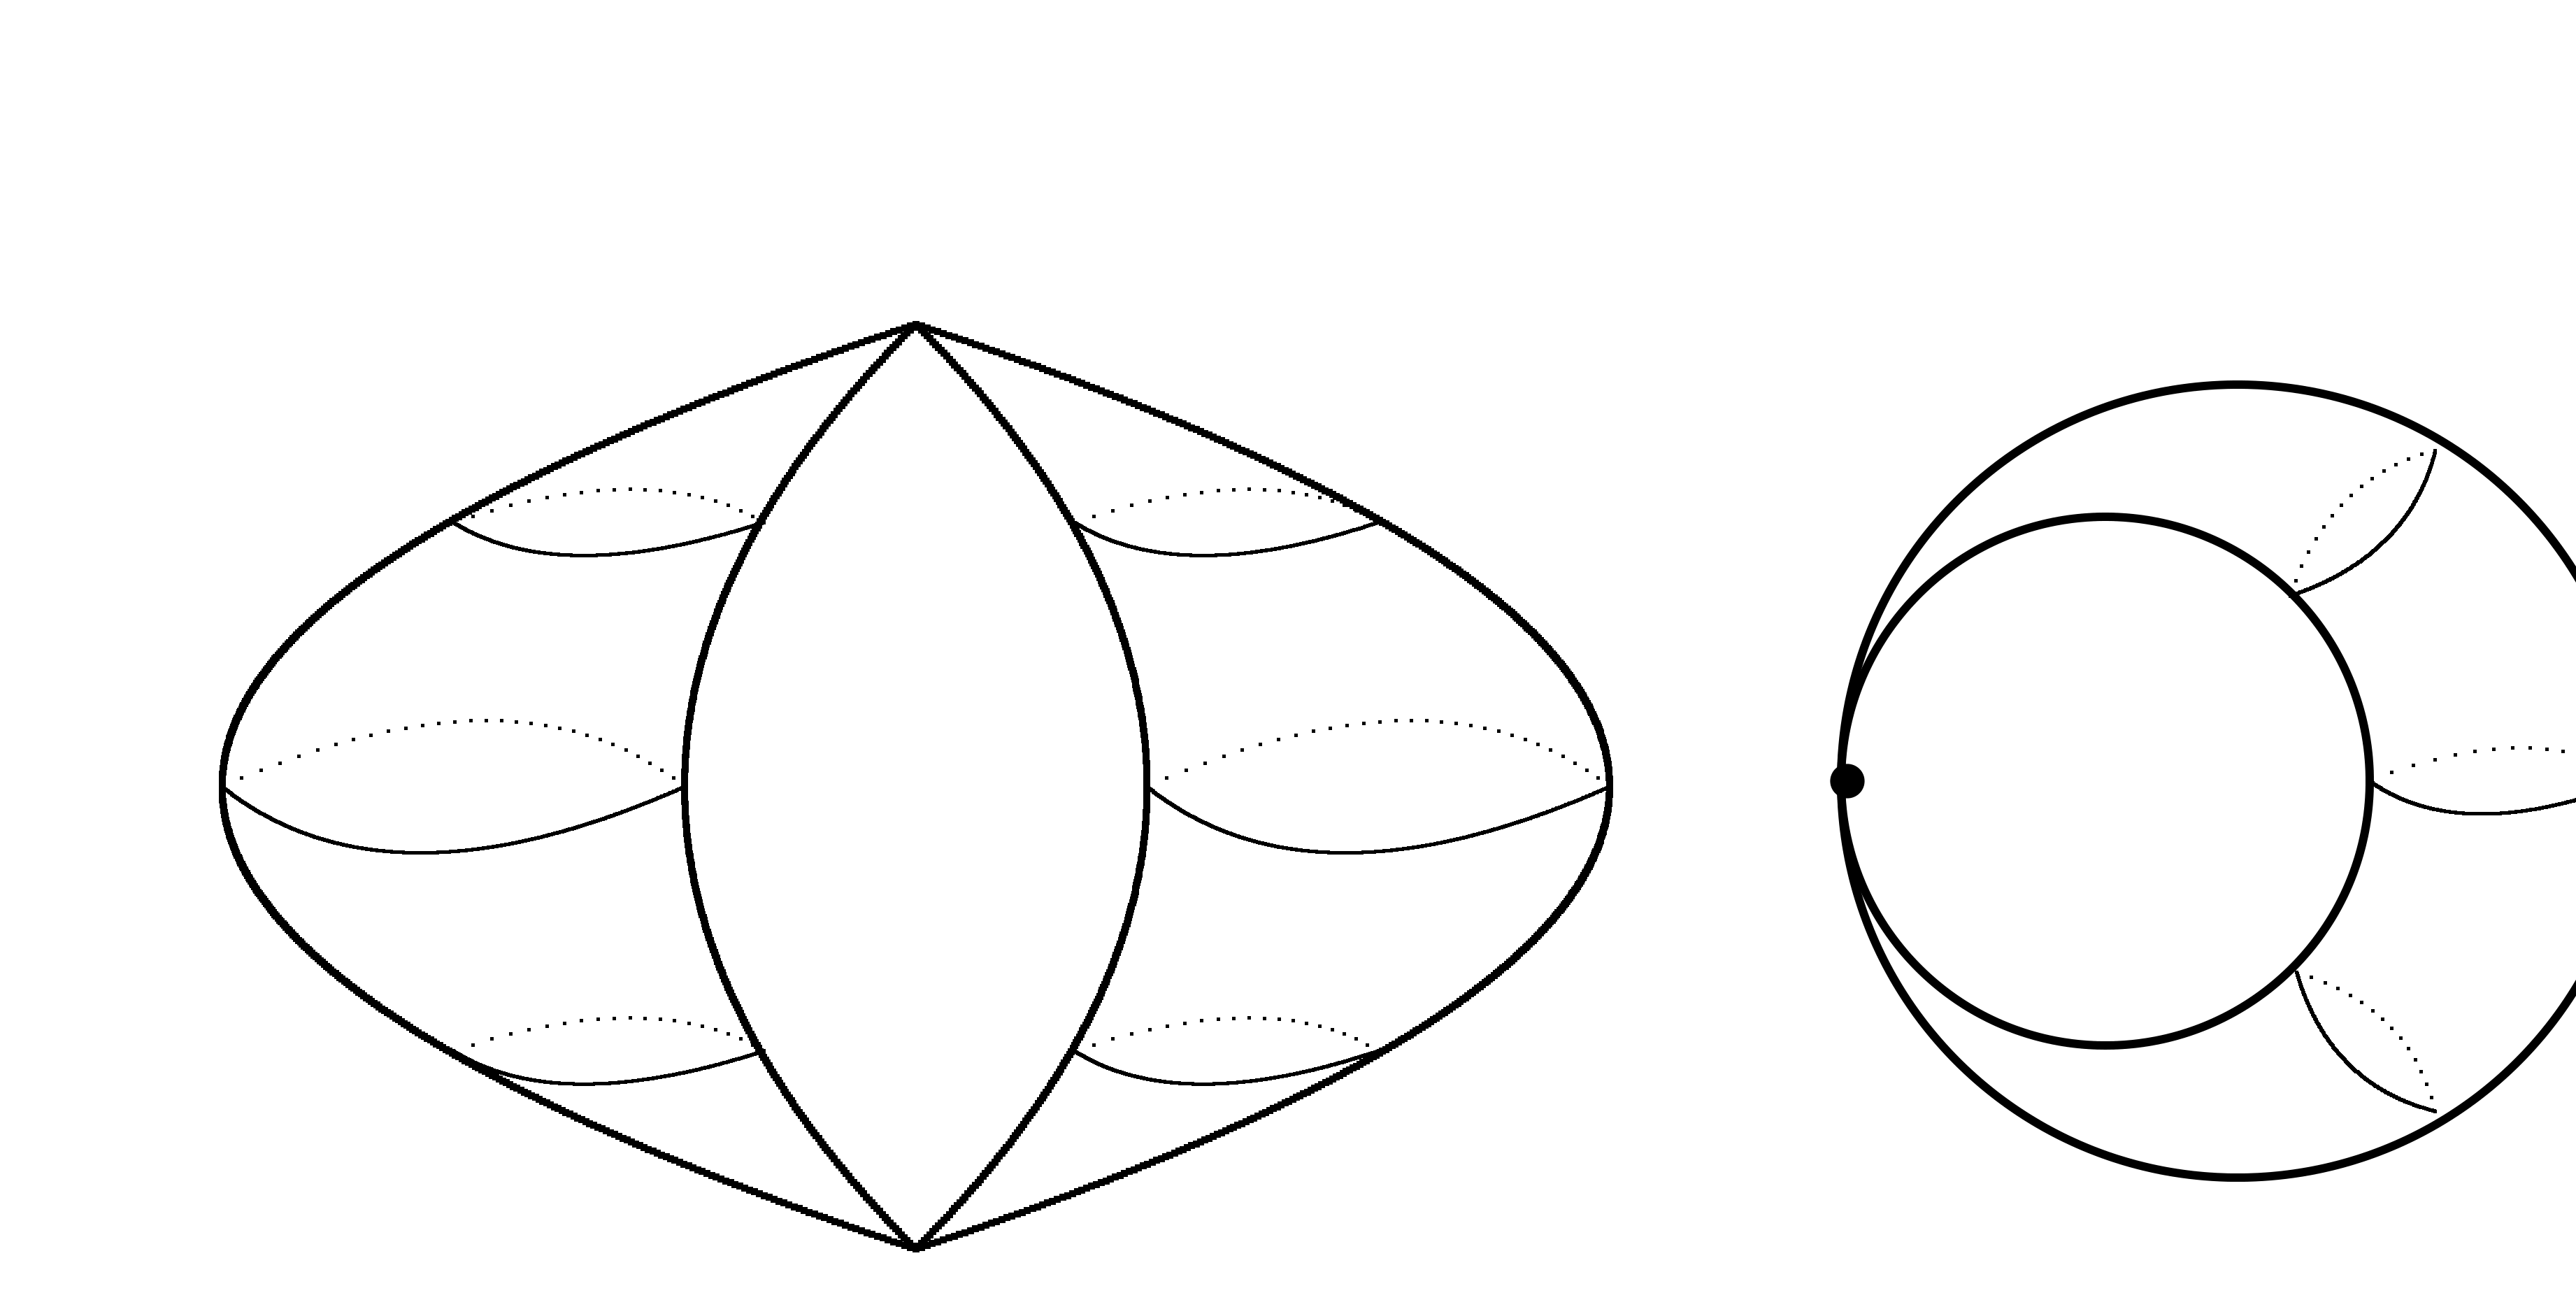
\includegraphics[width=0.92\textwidth]{figures/fig-p18-hitchin-fibers.png}
\caption{奇异 Hitchin 纤维。左：$A$-模型一侧，$G=SL_2$；右：$B$-模型一侧，${}^{L}G=SO_3$。（原书 p.18；原图无编号）}
\label{fig:p18-hitchin-fibers}
\end{figure}

尽管本文的细致分析将限于 ${}^{L}G=SO_3$、$G=SL_2$，我们的猜想是：对内窥的类似几何描述对所有群都成立（见第 9 节）。

\subsection{从 A-膜到 D-模}

至此所讨论的是 $\mathcal{M}_H(C;G)$ 上与 $\mathcal{M}_H(C;{}^{L}G)$ 上的 B-膜相对偶的 A-膜。然而，B-膜的几何 Langlands 对偶通常不是描述为 A-膜，而是描述为曲线 $C$ 上稳定 $G$-丛的模空间 $\mathcal{M}$（更一般地说，$C$ 上 $G$-丛的模叠 $\Bun_G$）上的扭 D-模。
% [Tutor Note: 易错预警。这里同时出现三个「模空间」：$\mathcal{M}_H$（Hitchin 模空间，超凯勒）、$\mathcal{M}$（稳定 $G$-丛的模空间，即 $\Bun_G$ 的稳定部分）、$T^*\mathcal{M}$（其余切丛）。原文用 $\mathcal{M}$ 而非 $\mathcal{M}_H$ 指后者，切勿与 Higgs 丛模空间混淆；$\mathcal{M}_H$ 只在非分歧情形才等于 $T^*\mathcal{M}$，有分歧时须换成仿射辛形变（见第 3.9 节）。]

这两种观点在 [KW] 第 11 节中得到调和。最熟悉的 A-膜是支撑在拉格朗日子流形（例如 Hitchin 纤维化的纤维）上、并带有平坦酉联络的膜。然而，辛流形 $X$ 上的 A-模型一般 [KO] 还可以有额外的膜，它们支撑在维数可能超过 $X$ 的一半维数的余迷向子流形上。特别地，设 $X=T^*Y$ 是复流形 $Y$ 的余切丛，带有自然的全纯二形式 $\Omega$。考虑 $X$ 上以辛形式 $\omega=\operatorname{Im}\Omega$ 定义的 A-模型。该 A-模型容许一个特殊的膜，即典范余迷向 A-膜 $\mathcal{A}_{cc}$，其支撑是整个 $X$，其存在弥合了 A-膜与 D-模之间的鸿沟。$\mathcal{A}_{cc}$ 的自同态（用物理术语说，即 $\mathcal{A}_{cc}-\mathcal{A}_{cc}$ 弦）可以沿 $Y$ 层化，给出一个环层。这个环层就是作用在 $K_Y^{1/2}$ 上的微分算子层，其中 $K_Y$ 是 $Y$ 的典范丛。我们以 $\mathcal{D}^*$ 记这样的微分算子层，并把此环层上的模层（或下文引入的其推广）称为扭 D-模。现在，若 $\mathcal{A}$ 是任何其它 A-膜，则 $\operatorname{Hom}(\mathcal{A}_{cc},\mathcal{A})$ 可以沿 $\mathcal{M}$ 层化，给出一个扭

% ==== 原文 PDF 第 19 页（印刷页 19）====

D-模。对应 $\mathcal{A}\to\operatorname{Hom}(\mathcal{A}_{cc},\mathcal{A})$ 给出一个从 A-膜范畴到扭 D-模范畴的函子。
% [Tutor Note: 推导补足。为什么自同态层给出「作用在 $K_Y^{1/2}$ 上的微分算子」？因为 $\mathcal{A}_{cc}$ 的支撑是整个 $X$，其开弦态空间在 $T^*Y$ 上局部由多项式函数（沿纤维方向）张成，沿 $Y$ 层化后得到 Weyl 代数层；再对 $Y\subset T^*Y$ 的横截方向作半无限形式的量子化（或等价地取 Weyl 代数的中心化子），即得作用在 $K_Y^{1/2}$ 上的微分算子层。$K_Y^{1/2}$ 的出现是半密度/半形式的必然结果，也是整篇「A-膜到 D-模」对应中唯一依赖 $Y$ 的几何信息之处。]

要把这一点应用到 $\mathcal{M}_H$ 上的 A-膜，我们注意到：虽然 $\mathcal{M}_H$ 并不恰好是余切丛，它含有一个可与 $T^*\mathcal{M}$ 等同的 Zariski 开集，其中 $\mathcal{M}$ 是稳定丛的模空间。$\mathcal{M}_H$ 上的 A-膜 $\mathcal{A}$ 可以限制到 $T^*\mathcal{M}$，而且由于维数理由这一限制非空。于是可以应用上述构造，把 $\mathcal{A}$ 联系到 $\mathcal{M}$ 上的扭 D-模。
% [Tutor Note: 易错预警。「由于维数理由限制非空」指的是：$\mathcal{A}$ 的支撑是实维数 $\ge\dim_{\mathbb{R}}\mathcal{M}_H$ 的余迷向子流形（拉格朗日膜恰为一半维数），而 $\mathcal{M}_H\setminus T^*\mathcal{M}$ 的余维为正，故支撑必与 $T^*\mathcal{M}$ 相交。这一步在原文中被一笔带过，但它是「A-膜总能给出 D-模」的关键；若支撑整个落在例外除子上，构造就会失效，而这里不会发生。]

这一构造有一个类比，其中 $X$ 不是 $Y$ 的余切丛，而是它的仿射辛形变。这意味着 $X\to Y$ 是仿射空间的丛，带有全纯辛形式 $\Omega$，使得沿 $Y$ 局部地 $X$ 等价于 $T^*Y$。这样的 $X$ 可由 $T^*Y$ 经元素\footnote{为构造 $X$，把 $\chi$ 拉回到 $H^1(T^*Y,\Omega^{1,\mathrm{cl}}(T^*Y))$，并用 $T^*Y$ 的辛形式把这个拉回映到 $H^1(T^*Y,T(T^*Y))$，后者分类 $T^*Y$ 的形变。所得形变是辛的，因为我们从 $\Omega^{1,\mathrm{cl}}$ 出发。}$\chi\in H^1(Y,\Omega^{1,\mathrm{cl}})$ 扭转得到，其中 $\Omega^{1,\mathrm{cl}}$ 是 $Y$ 上闭一形式的层。在这种情形，仍然可以定义\footnote{需要要求 $\operatorname{Re}\chi$ 的上同调类等于 [GW] 中称为 $\eta$ 的量子参数。除第 4.7 节外，我们强调经典图景并略去 $\eta$ 的作用。}典范余迷向膜 $\mathcal{A}_{cc}$，而 $\mathcal{A}_{cc}$ 的自同态仍然可以沿 $Y$ 层化。此时所得的环层是作用在 $K_Y^{1/2}\otimes\mathcal{L}$ 上的微分算子层，其中\footnote{一般地，$\chi$ 的上同调类不是整的，所以 $\mathcal{L}$ 可能是线丛的复幂（或这种幂的张量积），而不是普通的复线丛。但作用在 $\mathcal{L}$ 上、或作用在 $K_Y^{1/2}\otimes\mathcal{L}$ 上的微分算子层仍然有意义。}$\mathcal{L}$ 是一个「线丛」，满足 $c_1(\mathcal{L})=\chi$。于是我们得到一个从 $Y$ 上 A-膜到 $\mathcal{D}^*(\mathcal{L})$ 的模的函子，其中 $\mathcal{D}^*(\mathcal{L})$ 是作用在 $K_Y^{1/2}\otimes\mathcal{L}$ 上的微分算子层。

这一构造在 [KW] 中被应用于数学上所谓的量子几何 Langlands。（这里需要考虑取复结构为对 $I$ 作超凯勒旋转所得复结构下的 $X=\mathcal{M}_H$。）与我们的目的更相关的是，它被 [GW] 应用于几何 Langlands 的分歧情形。这里用到的事实是：在分歧情形，$\mathcal{M}_H$ 中的一个 Zariski 开集可以等同于 $T^*\mathcal{M}$ 的一个仿射辛形变。（对本文的例子，这在第 3.9 节有详细描述。）对几何 Langlands 的分歧情形，这一构造导致如下陈述：存在一个从 $\mathcal{M}_H(C;G)$ 的 A-膜到 $\mathcal{M}$ 上 $\mathcal{D}^*(\mathcal{L})$-模的自然函子，其中 $\mathcal{M}$ 现在是 $C$ 上稳定抛物 $G$-丛的模空间，而 $\mathcal{L}$ 的第一陈类是对偶 ${}^{L}G$ 局部系统的单值的对数。

\subsubsection{与局部系统的关系}

现在讨论在此情形中由 A-膜产生的扭 D-模如何与局部系统相联系。设 $X$ 为 $T^*Y$ 或其一仿射形变，并设 $\pi:X\to Y$ 为投影。设 $L$ 是 $X$ 的一个紧（复）拉格朗日子流形，使得映射 $\pi:L\to Y$ 是 $n$ 重覆盖。那么从 A-膜到扭 D-模的函子预期把支撑在 $L$ 上的秩 1 A-膜映为 $Y$ 上秩 $n$ 的局部系统（被 $K_Y^{1/2}$ 扭），换言之，映为 $Y$ 上带有平坦联络（或在仿射形变情形带有中心曲率联络）的秩 $n$ 复向量丛 $V\to Y$。

% ==== 原文 PDF 第 20 页（印刷页 20）====

若 $L$ 在 $X$ 中闭而不紧，且映射 $\pi:L\to Y$ 一般地是 $n$ 对 1、但在一个除子上次数较低，则上述结论有一个重要的推广。这在直观上发生的情形是：$L$ 的某些分支在所论除子之上趋于无穷远。为简单起见，假设 $Y$ 是曲线，第 3 节的例子实际上就是这种情况。设 $u$ 是 $Y$ 上的局部参数，设 $s$ 是 $X\to Y$ 的纤维上的线性函数，使得沿 $Y$ 局部地 $X$ 的辛形式为 $\Omega=du\wedge ds$。则 $L$ 可以局部地由一个 $n$ 值函数 $s(u)$ 描述，而我们所关心的情形是这个函数的某些分支在点 $r\in Y$（对应于比如 $u=u_0$）处奇异。我们假设这 $n$ 个分支形如
\begin{equation}\tag{2.6}
s_i(u)\sim c_i(u-u_0)^{-d_i},\qquad i=1,\dots,n.
\end{equation}
（$d_i$ 不必是整数，因为映射 $\pi:L\to Y$ 可能在 $u=u_0$ 处分歧。）在这种情形，支撑在 $L$ 上的 A-膜将映为 $Y$ 上的扭 D-模，后者由在 $r$ 处带奇点的局部系统 $V\to Y\setminus\{r\}$ 表示。奇点的性质在很大程度上由 $d_i$ 与 $c_i$ 决定。例如，正则奇点的条件是 $d_i\le 1$，而正则奇点处的单值也在很大程度上由 $c_i$ 决定。由于这个原因，我们在式 (3.49) 中为本文的例子计算 $c_i$ 与 $d_i$。在第 4 节中，我们解释这些系数预期如何与局部系统的奇点相联系，并描述向高维的推广。
% [Tutor Note: 易错预警。(2.6) 中的 $d_i$ 与 $c_i$ 互为独立的资料：$c_i$ 决定正则奇点处的单值（即共振项，经 $\exp(2\pi\ii c_i)$ 型公式），$d_i$ 决定奇点的阶（正则 vs 不规则）。条件 $d_i\le1$ 只是正则性的必要条件，真正的正则性还要看 $d_i$ 为整数时的对数项；原文只给出必要条件并说明「在很大程度上决定」，阅读时不可把 $d_i\le1$ 当作充分条件。]

\subsubsection{本征膜与本征层}

$\mathcal{M}_H$ 的镜像对称具有许多与它源自四维理论有关的特殊性质。例如，四维规范场论的 Wilson 与 't Hooft 线算子可以在二维意义下重新解释 [KW]，它们对于理解几何 Langlands 纲领的 Hecke 算子至关重要。

从 A-膜到 D-模的对应应当把 't Hooft 算子的本征 A-膜映为 $\mathcal{M}$ 上的 D-模（更一般地，映为曲线 $C$ 上 $G$-丛的模叠 $\Bun_G$ 上的 D-模），后者是 Hecke 本征层。这些 Hecke 本征层是几何 Langlands 对应（在其通常表述中）所关注的主要对象。几何 Langlands 猜想预言：对 $C$ 上每个 ${}^{L}G$-局部系统 $\mathcal{E}$，可以联系一个 $\Bun_G$ 上 Hecke 本征层的范畴 $\mathcal{A}ut_\mathcal{E}$。特别地，若该局部系统的自同构群平凡，则预期这个范畴等价于向量空间范畴。换言之，它含有一个唯一的不可约对象，而所有其它对象都是该对象的若干拷贝的直和。困难在于描述自同构群非平凡的局部系统所对应的情形。
% [Tutor Note: 物理图像。这里「范畴 $\mathcal{A}ut_\mathcal{E}$」正是几何 Langlands 猜想（[BD] 的原始形式）所断言的，它是 $\Bun_G$ 上满足 Hecke 本征性质的 D-模范畴。自同构群平凡时预期它 $\simeq\mathrm{Vect}$，其唯一不可约对象就是对应于 $\mathcal{E}$ 的 Hecke 本征层；自同构群非平凡时，正如 B-模型一侧的轨形点使点膜范畴变复杂，此处的范畴也随之变复杂，本文正是要显式描述这种复杂性（分数 Hecke 性质）。]

然而，用 D-模的语言来做这件事相当困难。在那些 Hecke 本征层已被显式构造出来的情形（例如 $G=SL_n$），其结构以复杂著称，这使得提取有用信息变得困难。另一方面，A-膜的语言则更适合于分析相应的本征膜范畴的结构。如上所述，一般的本征膜是光滑 Hitchin 纤维上的酉平坦局部系统，而与内窥相关的特殊本征膜则支撑在奇异 Hitchin 纤维上。结果表明，人们可以非常显式地描述这些奇异纤维，

% ==== 原文 PDF 第 21 页（印刷页 21）====

从而非常显式地描述相应的本征膜。例如，我们观察到支撑在奇异纤维上的本征膜分裂成若干片，即前面讨论过的「分数膜」。此外，这些分数膜满足本征膜性质的某种修正，该修正性质在第 5.3 节中讨论（分数本征膜性质）。

然后我们把这些结果翻译成 D-模的语言。于是，若本征膜 $\mathcal{A}$ 分解为两个不可约膜 $\mathcal{A}_1$ 与 $\mathcal{A}_2$，则自然地预测相应的 Hecke 本征层 $\mathcal{F}$ 也将分解为两个 D-模 $\mathcal{F}_1$ 与 $\mathcal{F}_2$ 的直和，分别对应于 $\mathcal{A}_1$ 与 $\mathcal{A}_2$。此外，这两个 D-模应当满足第 6 节所述的分数 Hecke 本征层性质。

这一切的要旨是：通过分析支撑在奇异 Hitchin 纤维上的 A-膜范畴，我们获得对几何 Langlands 对应的大量洞察，并且有望甚至对有限域上曲线的经典 Langlands 对应获得洞察。我们将在下面给出的显式例子中详细描述这一点。

% ============================================================
% 分片：s03a-genus1  对应原文 PDF 第 21--27 页（印刷页 21--27）
% 负责章节：§3 Explicit Example In Genus One + 3.1--3.5（§3 标题起）
% 译者：trans-s02   审校状态：初稿
% ============================================================

% ==== 原文 PDF 第 21 页（印刷页 21）====

\section{亏格一中的显式例子}

\begin{keytakeaway}
\textbf{核心物理图像：}在亏格 $1$、单分歧点的模型里，内窥的几何图像可以被完全显式地算出：B-模型一侧 ${}^{L}G=SO_3$ 的 Hitchin 模空间含 $4$ 个 $A_1$ 轨形奇点，对应自同构群为 $\mathbb{Z}_2$ 的内窥局部系统；A-模型一侧 $G=SL_2$ 的 Hitchin 模空间本身光滑，但在底中三个特殊点 $w=e_i$ 处的 Hitchin 纤维分裂为两条亏格 $0$ 曲线，正是内窥所需的奇异纤维。
\textbf{数学工具：}椭圆曲线 $y^2=f(x)=x^3+ax+b$ 上的分歧 $SL_2$ Higgs 丛、Hitchin 方程在极点附近的局部形式与单值公式、特征多项式 $\operatorname{Tr}\varphi^2$、$\mathbb{Z}_2$ 不变量 $\rho,y_0^2,h_0^2$ 与模空间方程 (3.15)、判别式与 $A_1$ 奇点的形变/消解、2 阶线丛群 $\mathcal{Q}=\mathbb{Z}_2\times\mathbb{Z}_2$ 在 Hitchin 底与纤维上的作用。
\textbf{主要结论：}对每个 $\sigma_0^2\neq 0$，分歧 $SL_2$ Higgs 丛的模空间是 (3.15) 所描述的复曲面，Hitchin 底由参数 $w$ 给出；三个奇异纤维 $w=e_i$ 各分裂为两个分支 $\boldsymbol{F}_{e_i}^{\pm}$，它们在两个二重点处相交；$\mathcal{Q}$ 通过 2 阶点的平移作用于每个纤维，其中 $T_1$ 保持两个分支不变并在二重点处有不动点，$T_2,T_3$ 在长方向上平移、忠实作用并交换两个分支与两个二重点。
\end{keytakeaway}

\subsection{亏格一的 Higgs 丛}

为构造一个能看出内窥的几何类比的显式例子，我们取 $G=SL_2$，并在亏格 $g_C=1$ 的 Riemann 面 $C$ 上工作，带有单个分歧点 $p$。人们或许会以为分歧会带来额外的复杂性，但事实上，亏格 $1$ 加单个分歧点的情形特别简单，在 Hitchin 纤维化的文献中常被考虑。对 $g_C\ge 2$，相应的模空间维数更高，显式计算困难；对 $g_C\le 1$，$C$ 的基本群是阿贝尔的（或平凡的），在没有分歧时会带来与内窥无关的复杂性，我们愿意在此避开。

正如我们在第 5.3 节所解释的，对 $g_C>1$，虽然显式计算困难，谱曲线方法是强有力的替代手段。但我们更愿意从 $g_C=1$ 的情形开始，因为此时一切都可以直接算出。

首先我们描述亏格 $1$ 的 Riemann 面 $C$ 上无分歧的 Higgs 丛。我们从通常的 $SL_2$ Higgs 丛开始，即对 $(E,\varphi)$，其中 $E$ 是行列式平凡的秩 $2$ 丛。若 $E$ 是半稳定的，它必须具有形式
\begin{equation}\tag{3.1}
E=\mathcal{L}\oplus\mathcal{L}^{-1}
\end{equation}
其中 $\mathcal{L}$ 是次数为 $0$ 的复线丛。若 $\mathcal{L}$ 非平凡，则 $\phi$ 在这个基下必须是
\begin{equation}\tag{3.2}
\phi=
\begin{pmatrix}
a & 0\\
0 & -a
\end{pmatrix}
\end{equation}
其中 $a$ 是 $C$ 上通常的全纯微分。$\mathcal{L}$ 的选择由一条与 $C$ 同构的曲线 $C'$（即 $C$ 的雅可比簇）参数化，而全纯微分空间是一维的。于是我们构造了由 $C'\times C$ 参数化的半稳定 Higgs 丛族，其中 $\mathcal{L}$ 的选择给出 $C'$ 中的点，$a$ 的选择给出 $C$ 中的点。（我们隐含地在 $C$ 上取定了一个特定的全纯微分，以把这样的微分空间等同于 $C$。）然而，把 $\mathcal{L}$ 换成 $\mathcal{L}^{-1}$
% [存疑: 原书 p.21 此句「若 $\mathcal{L}$ 非平凡，则 $\phi$ 必须在这个基下是」与紧接的 (3.2) 把 Higgs 场排作直立的 $\phi$，而同一页上一句的 $(E,\varphi)$ 与全书其余各处（含 (3.8)、(3.10)、(3.12) 等）均排作 $\varphi$。疑为原文记号不一致，此处照原样保留。]
% [Tutor Note: 推导补足。为何「半稳定」迫使 $E=\mathcal{L}\oplus\mathcal{L}^{-1}$？这是 Atiyah 对椭圆曲线上半稳定丛的分类：亏格 $1$ 上次数 $0$ 的半稳定丛必为其稳定部分的直和，而秩 $2$、行列式平凡的稳定部分只能是两个次数 $0$ 的线丛（稳定线丛即 $SL_2$ 丛的约化）。注意 $a$ 是 $C$ 上全纯微分（即 $H^0(C,K)$ 的元素），在 $C$ 上 $H^0(C,K)$ 一维，这正是后文可以只用一个复参数 $a$ 描述 Higgs 场的原因。]

% ==== 原文 PDF 第 22 页（印刷页 22）====

并改变 $a$ 的符号，会得到同一个 Higgs 丛（同构意义下）。这一操作可以理解为一个规范变换
\begin{equation}\tag{3.3}
\begin{pmatrix}
0 & 1\\
-1 & 0
\end{pmatrix}.
\end{equation}
于是我们可以取 $\mathbb{Z}_2$ 的商，得到由 $(C'\times C)/\mathbb{Z}_2$ 参数化的半稳定 Higgs 丛族。这实际上就是 $C$ 上行列式平凡的秩 $2$ 半稳定 Higgs 丛的模空间。

\subsection{分歧}

现在让我们把分歧纳入进来。在 Higgs 丛的语境中，分歧意味着 [Sim1] $\varphi$ 可以在一个指定的点 $p\in C$（或更一般地在若干这样的点）处有极点，并且其极点部分的特征多项式是预先指定的。我们将考虑单极点的情形。此外，在丛 $E$ 于 $p$ 处的纤维 $E_p$ 中，给定一个 $\varphi$-不变的抛物结构，即一个在 $\varphi$ 的极点部分的作用下不变的旗。此外，这个旗还带有抛物权。整个结构可以通过把 Hitchin 方程改造以纳入奇点而统一地描述。$p$ 附近的行为由取值于 $G$ 的紧实形式的极大环面的 Lie 代数 $\mathfrak{t}$ 中的参数 $\alpha,\beta,\gamma$ 决定。设 $z$ 是 $p$ 附近的局部参数，并写 $z=re^{\ii\theta}$。按 [GW] 的记号，$p$ 附近的局部行为为
\begin{equation}\tag{3.4}
\begin{aligned}
A &= \alpha\, d\theta + \ldots\\
\phi &= \beta\,\frac{dr}{r} - \gamma\, d\theta + \ldots .
\end{aligned}
\end{equation}

由于 Higgs 场 $\varphi$ 正是 $\phi$ 的 $(1,0)$ 部分，这些方程立即决定了它的极点行为（差一个规范等价或共轭）。有 $\varphi\sim\sigma\, dz/z$，其中 $\sigma=(\beta+\ii\gamma)/2$。$\varphi$-不变的抛物结构完全由 $\varphi$ 以及一个包含 $\sigma$ 的 Borel 子群的选择决定。若 $\sigma$ 是正则的（我们将一般地这样假设），则包含 $\sigma$ 的 Borel 子群只有有限多个选择，而选择可由对 $\sigma$ 的特征值排序来确定。因此，在研究具有正则 $\sigma$ 的分歧 Higgs 丛时，抛物结构（或 $\alpha$ 的选择）不需要显式指定。
% [Tutor Note: 推导补足。$\sigma=(\beta+\ii\gamma)/2$ 与 $\varphi\sim\sigma\, dz/z$ 来自把实一形式投影到 $(1,0)$ 部分：取 $z=re^{\ii\theta}$、平坦度量 $|dz|^2$，则 $\star(dr/r)=d\theta$、$\star(d\theta)=-dr/r$，$(1,0)$ 投影为 $\tfrac12(1+\ii\star)$，作用于 $\phi=\beta\,dr/r-\gamma\,d\theta$ 得 $\tfrac12(\beta+\ii\gamma)(dr/r+\ii\,d\theta)=\sigma\,dz/z$。这也解释了为何 $\sigma$ 的两个特征值 $\pm\sigma_0$ 会在 (3.11) 中以 $\sigma_0^2$ 的形式进入特征多项式。]

类似地，我们可以确定具有联络 $\mathcal{A}=A+\ii\phi$ 的局部系统绕 $p$ 的单值。它是
\begin{equation}\tag{3.5}
M=\exp(-2\pi(\alpha-\ii\gamma)).
\end{equation}
% [存疑: 按同一页上文 $\mathcal{A}=A+\ii\phi$ 与 (3.4) 的局部形式直接计算，绕 $p$ 一圈给出 $\exp(+2\pi(\alpha-\ii\gamma))$（取 $z=re^{\mathrm{i}\theta}$、逆时针绕行），而 (3.5) 带有负号。此符号应来自单值的朝向约定（例如把单值定义为 $\exp(-\oint\mathcal{A})$ 或取反向绕行），原书未加说明；此处照原样保留。]

现在让我们特殊化到亏格 $1$、带一个分歧点的曲线 $C$ 的情形。用代数方程显式描述 $C$ 是方便的：
\begin{equation}\tag{3.6}
y^2=f(x)
\end{equation}
其中我们可以取 $f$ 形如
\begin{equation}\tag{3.7}
f(x)=x^3+ax+b
\end{equation}
并把 $p$ 解释为无穷远点。我们假设 $f$ 的根互不相同，从而 $C$ 光滑。
% [Tutor Note: 易错预警。(3.6) 中的 $(x,y)$ 是 $C$ 上的亚纯函数，$x$ 在无穷远点 $p$ 处有 $2$ 阶极点、$y$ 有 $3$ 阶极点，这正是后文「$x\sim z^{-2}$、$y\sim z^{-3}$」的来源。另注意字母 $a$ 被原书复用：在 (3.2) 中 $a$ 是 $C$ 上的全纯微分（即 $H^0(C,K)$ 的元素），而在 (3.7) 中 $a$ 是椭圆曲线方程的常数系数；阅读 (3.9)--(3.12) 时须分清这两处 $a$。]

% ==== 原文 PDF 第 23 页（印刷页 23）====

为显式描述分歧 Higgs 丛 $(E,\varphi)$，我们先像以前一样取 $E=\mathcal{L}\oplus\mathcal{L}^{-1}$，其中 $\mathcal{L}$ 次数为零。我们可以取 $\mathcal{L}=\mathcal{O}(p)\otimes\mathcal{O}(q)^{-1}$，其中 $q$ 是 $C$ 中某个点，对应于 $(x,y)=(x_0,y_0)$。Higgs 场将具有形式
\begin{equation}\tag{3.8}
\varphi=
\begin{pmatrix}
h & k\\
g & -h
\end{pmatrix},
\end{equation}
其中 $h$ 是 $K\otimes\mathcal{O}(p)$ 的截面，$k$ 是 $K\otimes\mathcal{O}(p)\otimes\mathcal{L}^2$ 的截面，$g$ 是 $K\otimes\mathcal{O}(p)\otimes\mathcal{L}^{-2}$ 的截面。当然，对亏格 $1$ 的 $C$，$K$ 由微分 $dx/y$ 平凡化。相应的线丛都具有一维的全纯截面空间，而 $k,g,h$ 的一般形式为
\begin{equation}\tag{3.9}
\begin{aligned}
h &= \frac{dx}{y}h_0\\
k &= \frac{dx}{y}k_0\left((y-y_0)-\frac{f'(x_0)(x-x_0)}{2y_0}\right)\\
g &= \frac{dx}{y}g_0\left((y+y_0)+\frac{f'(x_0)(x-x_0)}{2y_0}\right)\frac{1}{(x-x_0)^2}.
\end{aligned}
\end{equation}
其中 $h_0,k_0,g_0$ 是复常数，而这些公式是这样得到的。$h$ 的公式无需解释。把 $K$ 平凡化之后，$k$ 应当是 $\mathcal{O}(p)\otimes\mathcal{L}^2=\mathcal{O}(p)^3\otimes\mathcal{O}(q)^{-2}$ 的全纯截面，所以我们寻找一个除在无穷远处有三阶极点之外全纯、并且在 $q$ 处有二阶零点的函数。这样的函数是 $(y-y_0)-f'(x_0)(x-x_0)/2y_0$。类似地，$g$ 应当是 $\mathcal{O}(p)\otimes\mathcal{L}^{-2}=\mathcal{O}(p)^{-1}\otimes\mathcal{O}(q)^2$ 的全纯截面，所以我们寻找一个除在 $q$ 处有二阶极点之外全纯、并在无穷远处消失的函数。这样的函数是 $\left((y+y_0)+\frac{f'(x_0)(x-x_0)}{2y_0}\right)/(x-x_0)^2$。
% [Tutor Note: 推导补足。这里隐含的计数是：$\mathcal{L}=\mathcal{O}(p)\otimes\mathcal{O}(q)^{-1}$ 给出 $\mathcal{L}^2=\mathcal{O}(2p)\otimes\mathcal{O}(q)^{-2}$，故 $\mathcal{O}(p)\otimes\mathcal{L}^2=\mathcal{O}(3p)\otimes\mathcal{O}(q)^{-2}$；而在亏格 $1$ 上 $h^0(\mathcal{O}(3p)\otimes\mathcal{O}(q)^{-2})=3-2+1-1=1$（Riemann--Roch 且 $h^1=0$），所以截面唯一到常数倍，这正是 $k_0$ 这个自由常数的由来。$g$ 的情形同理：$\deg(\mathcal{O}(p)\otimes\mathcal{L}^{-2})=-1$，$h^0(-p+2q)= -1+2+1-1=1$。$\mathcal{O}(p)^3$ 是 $\mathcal{O}(3p)$ 的简写。]

下一步是计算 $\varphi$ 的特征多项式。对 $G=SL_2$，这简单地意味着我们应当计算 $\operatorname{Tr}\varphi^2$，而在当前情形它结果为
\begin{equation}\tag{3.10}
\operatorname{Tr}\varphi^2=\left(\frac{dx}{y}\right)^2\left(2h_0^2+2k_0g_0\left(x+2x_0-\frac{f'(x_0)^2}{4f(x_0)}\right)\right).
\end{equation}
$\operatorname{Tr}\varphi^2$ 的极点部分简单地是 $(dx/y)^2 2xk_0g_0$，它在无穷远处有二阶极点。若 $z$ 是无穷远处的局部参数，我们有 $x\sim z^{-2}$、$y\sim z^{-3}$，且 $(dx/y)^2x\sim 4(dz/z)^2$。$\varphi$ 的极点部分应当共轭于 $\sigma dz/z$，所以我们要求 $\operatorname{Tr}\varphi^2\sim\operatorname{Tr}\sigma^2(dz/z)^2=2\sigma_0^2(dz/z)^2$，其中我们把 $\sigma$ 的特征值记作 $\pm\sigma_0$。于是我们令 $k_0g_0=\sigma_0^2/4$，并写出
\begin{equation}\tag{3.11}
\operatorname{Tr}\varphi^2=\left(\frac{dx}{y}\right)^2\left(2h_0^2+\frac{\sigma_0^2}{2}\left(x+2x_0-\frac{f'(x_0)^2}{4f(x_0)}\right)\right).
\end{equation}
% [Tutor Note: 推导补足。(3.10) 中被跳过的一步是一个三次恒等式：对 $f(x)=x^3+ax+b$ 有 $f(x)-f(x_0)-f'(x_0)(x-x_0)=(x-x_0)^2(x+2x_0)$。把 (3.9) 代入 $\operatorname{Tr}\varphi^2=2h^2+2kg$ 后，$kg$ 含因子 $\left[(y-y_0)(y+y_0)-\frac{f'(x_0)^2(x-x_0)^2}{4y_0^2}\right]/(x-x_0)^2$，利用 $y^2=f(x)$、$y_0^2=f(x_0)$ 及上述恒等式即得 (3.10)。再由 $x\sim z^{-2}$、$y\sim z^{-3}$ 得 $\frac{dx}{y}\sim -2\,\frac{dz}{z}$，故 $(dx/y)^2x\sim 4(dz/z)^2$，这正是定出 $k_0g_0=\sigma_0^2/4$ 的依据。]
% [Tutor Note: 易错预警。(3.10)--(3.11) 中的 $f(x_0)$ 出现在分母，因此在 $f(x_0)=0$（即 $y_0=0$）处公式失效；这也正是下文「$y_0=0$ 或 $y_0=\infty$ 时 (3.9) 失效」的代数根源。另注意 $\operatorname{Tr}\varphi^2$ 作为 Hitchin 映射的分量，其归一化依赖 $\sigma$ 的特征值差：$\operatorname{Tr}\sigma^2=2\sigma_0^2$，若把特征值写成 $\pm\sigma_0$ 则系数 $2$ 不可漏掉。]

只有乘积 $k_0g_0$ 被确定，其原因在于丛 $E=\mathcal{L}\oplus\mathcal{L}^{-1}$ 有自同构群 $\mathbb{C}^\times$，它分别在两个直和项上作用为乘以 $\lambda$ 与 $\lambda^{-1}$，并把 $k_0$ 与 $g_0$ 变换为 $k_0\to\lambda^2k_0$、$g_0\to\lambda^{-2}g_0$。

公式 (3.9) 在 $y_0=0$ 时失效（因为 $y_0$ 出现在 $k$ 与 $g$ 的公式的分母中），或者在 $y_0=\infty$ 时失效（因为 $k$ 与 $g$ 的公式还含有关于 $y_0$ 线性的项），等价地，在 $\mathcal{L}$ 为 $2$ 阶时失效。发生这种情况是因为当 $\mathcal{L}$

% ==== 原文 PDF 第 24 页（印刷页 24）====

为 $2$ 阶时，我们有 $\mathcal{L}\cong\mathcal{L}^{-1}$，并且（若 $\sigma\ne 0$）不存在稳定的或半稳定的分歧 Higgs 丛 $(E,\varphi)$ 满足 $E=\mathcal{L}\oplus\mathcal{L}^{-1}=\mathcal{L}\oplus\mathcal{L}$。事实上，取这样的 $E$，$K\otimes\mathrm{ad}(E)\otimes\mathcal{O}(p)\cong K\otimes\mathcal{O}(p)^{\oplus 3}$ 的全纯截面在 $p$ 处不可能有极点，从而条件 $\operatorname{Tr}\varphi^2\sim 2\sigma_0^2(dz/z)^2$ 无法被满足。反之，若 $\mathcal{L}$ 为 $2$ 阶且 $\sigma\ne 0$，则必须取 $E$ 为 $\mathcal{L}$ 被 $\mathcal{L}$ 的非平凡扩张。
% [Tutor Note: 推导补足。「不可能有极点」是次数计算：$\mathcal{L}^2\cong\mathcal{O}$ 时 $\mathrm{ad}(E)\cong\mathcal{O}^{\oplus 3}$，故 $K\otimes\mathrm{ad}(E)\otimes\mathcal{O}(p)\cong K\otimes\mathcal{O}(p)^{\oplus 3}$；而 $\deg(K\otimes\mathcal{O}(p))=2g-2+1=1$，由 Riemann--Roch 得 $h^0=1$、$h^1=0$，其全纯截面（到常数倍）由 $dx$ 给出、在 $p$ 处正则，不可能带有极点，与 $\operatorname{Tr}\varphi^2$ 在 $p$ 处有二阶极点矛盾。这正是为何 $\mathcal{L}$ 为 $2$ 阶时必须改用非平凡扩张。]

\subsection{模空间}

对参数 $\sigma_0^2$ 的每个选择，我们构造了一个分歧 Higgs 丛族。底丛是 $E=\mathcal{L}\oplus\mathcal{L}^{-1}$，而 Higgs 场 $\varphi$ 已如上描述。$E$ 的选择依赖于点 $q$，或等价地依赖于对 $(x_0,y_0)$（满足 $y_0^2=f(x_0)$），而 $\varphi$ 的选择还额外依赖于参数 $h_0$。要在这种情况下构造分歧 Higgs 丛的模空间 $\mathcal{M}_H$，我们必须考虑对换 $\tau:\mathcal{L}\to\mathcal{L}^{-1}$，它作用为 $(x_0,y_0,h_0)\to(x_0,-y_0,-h_0)$。

对 $(q,h_0)$ 或三元组 $(x_0,y_0,h_0)$ 定义了 $C\times C$ 中的一个点，而在容许对称 $\tau$ 之后，模空间似乎是 $(C\times C)/\mathbb{Z}_2$，与 $\sigma_0$ 无关。这实际上并不完全正确，原因在于第 3.2 节末尾所指出的那一点。空间 $(C\times C)/\mathbb{Z}_2$ 有四个 $A_1$ 奇点，位于 $h_0=0$ 且 $q$ 为 $2$ 阶的点处。对 $\sigma\ne 0$，$A_1$ 奇点被形变，模空间变得光滑。我们没有看到这一形变，因为我们的分析没有覆盖 $q$ 为 $2$ 阶的情形。若 $\sigma=0$ 而 $\alpha\ne 0$，则 $A_1$ 奇点是被消解而不是被形变；从超凯勒的观点看，对 $\sigma$ 与 $\alpha$ 的一般取值，这一现象实际上是同时的形变与消解，如 [Kr] 中那样。本文不会直接描述这一形变或消解，但在下文方程 (3.15) 中，借助 Hitchin 纤维化描述了形变后的模空间。
% [Tutor Note: 易错预警。这里区分了两种局部模型：$A_1$ 奇点的**形变**（deformation，$\sigma\ne 0$，对应复结构 $I$ 下一族光滑超凯勒流形）与**消解**（resolution，$\sigma=0$ 而 $\alpha\ne 0$，对应把 $\mathbb{C}^2/\mathbb{Z}_2$ 的奇点用一条 $\mathbb{P}^1$ 替换）。原文说对一般 $(\sigma,\alpha)$ 是「同时的形变与消解」，这正是超凯勒旋转下的图像：$I$ 下看到的形变与 $J$ 下看到的消解由同一个超凯勒度量联系起来（[Kr]）。切勿把二者混为一谈，也别把 (3.15) 误当作消解后的空间——它只描述形变。]

这里或许应当就分歧在亏格 $1$ 中的作用作一点评论。对 $g_C>1$，一般的半稳定丛实际上是稳定的；但对 $g_C=1$（且无分歧）以及单连通的 $G$，不存在严格稳定的丛。最接近的是半稳定丛，例如 $G=SL_2$ 时的 $E=\mathcal{L}\oplus\mathcal{L}^{-1}$。同样地，一般地 $\mathcal{M}_H$ 参数化稳定与半稳定 Higgs 丛。对 $g_C=1$，无分歧的 Higgs 丛充其量是半稳定的，所以 $\mathcal{M}_H$ 实际上参数化半稳定 Higgs 丛。有了分歧，情况就变了。带一个分歧点的半稳定 Higgs 丛实际上是稳定的（若 $\sigma\ne 0$）。其原因在于 $E=\mathcal{L}\oplus\mathcal{L}^{-1}$ 的潜在失稳层（即直和项 $\mathcal{L}$ 与 $\mathcal{L}^{-1}$）不是 $\varphi$-不变的，因此不违反 Higgs 丛 $(E,\varphi)$ 的稳定性。

\subsection{Hitchin 纤维化}

接下来我们需要理解 Hitchin 纤维化。Hitchin 纤维化就是把 Higgs 丛 $(E,\varphi)$ 映到 $\varphi$ 的特征多项式的映射。对 $G=SL_2$，这个特征多项式约化为 $\operatorname{Tr}\varphi^2$。在当前语境中，按 (3.11)，该特征多项式是 $x$ 的一次多项式（乘以 $(dx/y)^2$）。$x$ 的一次项系数是固定的，而 Hitchin 纤维化就是提取常数项的映射，我们把这个常数项记作 $w_0$。换言之，Hitchin 纤维化把 Higgs 丛 $(E,\varphi)$ 映到
\begin{equation}\tag{3.12}
w_0=2h_0^2+\frac{\sigma_0^2}{2}\left(2x_0-\frac{f'(x_0)^2}{4f(x_0)}\right).
\end{equation}

% ==== 原文 PDF 第 25 页（印刷页 25）====

Hitchin 纤维化的纤维由满足 (3.12) 与
\begin{equation}\tag{3.13}
y_0^2=f(x_0)
\end{equation}
的变量 $x_0,y_0,h_0$ 描述，并且还受 $\mathbb{Z}_2$ 对称 $(x_0,y_0,h_0)\to(x_0,-y_0,-h_0)$ 的作用。除 $x_0$ 之外，$\mathbb{Z}_2$ 不变量是 $y_0^2$、$h_0^2$ 以及
\begin{equation}\tag{3.14}
\rho=(2/\sigma_0)y_0h_0.
\end{equation}
（因子 $2/\sigma_0$ 是为方便而引入的。）其中，按最后两个方程，$y_0^2$ 与 $h_0^2$ 等价于 $x_0$ 的有理函数，因而可以略去；而 $\rho$ 满足一个二次方程。若此后我们把 $x_0$ 写作 $u$，并令 $w_0=-w\sigma_0^2/2$，则 $\rho$ 所满足的方程为
\begin{equation}\tag{3.15}
\rho^2=-(2u+w)f(u)+\frac{f'(u)^2}{4}.
\end{equation}
% [Tutor Note: 推导补足。(3.15) 由 (3.12)--(3.14) 消去 $x_0,y_0,h_0$ 得到，关键一步是：由 (3.12) 解出 $h_0^2=\frac{w_0}{2}-\frac{\sigma_0^2}{4}\left(2u-\frac{f'(u)^2}{4f(u)}\right)$，代入 (3.14) 得 $\rho^2=\frac{4}{\sigma_0^2}y_0^2h_0^2=\frac{4}{\sigma_0^2}f(u)h_0^2$；再用 $w_0=-w\sigma_0^2/2$ 化简，$\sigma_0^2$ 恰好约去，即得 (3.15)。这也解释了原书为何强调 $\sigma_0$ 不出现：$\sigma_0$ 可通过重新标度 $\varphi$ 消去，(3.15) 只依赖 $w$ 与 $u$。]

关于复变量 $\rho,u,w$ 的这个方程描述了一个复曲面，它就是分歧 $SL_2$ Higgs 丛的模空间 $\mathcal{M}_H$。（在这种写法中，$u,\rho=\infty$ 处的某些点被略去了。）有一个简单的解释说明它为何不依赖于刻画分歧的参数 $\alpha,\beta,\gamma$。复结构 $I$ 不依赖 $\alpha$，而只要只有一个分歧点，$\sigma=(\beta+\ii\gamma)/2$ 就可以通过重新标度 $\varphi$ 消去（只要它不为零），正如我们所做的那样。

若把 $w$ 取为固定的复数，我们得到一条代数曲线 $\boldsymbol{F}_w$，它是 Hitchin 纤维化的纤维。右端是关于 $u$ 的四次多项式，并且对一般的 $w$，$\boldsymbol{F}_w$ 是亏格 $1$ 的光滑曲线。

$\boldsymbol{F}_w$ 何时奇异？这恰好发生在多项式 $g(u)=(2u+w)f(u)-f'(u)^2/4$ 的两个根重合时，换言之，在其判别式为零时。设 $e_1,e_2,e_3$ 是多项式 $f(u)=u^3+au+b$ 的根。（当然 $e_1+e_2+e_3=0$，并且我们假设 $e_i$ 互不相同，从而 $C$ 光滑。）$g$ 的判别式为 $(e_1-e_2)^2(e_2-e_3)^2(e_3-e_1)^2(w-e_1)^2(w-e_2)^2(w-e_3)^2$，所以 $\boldsymbol{F}_w$ 奇异恰好当 $w$ 等于某个 $e_i$。例如，若 $w=e_1$，我们发现
\begin{equation}\tag{3.16}
-(2u+w)f(u)+\frac{f'(u)^2}{4}=\frac{1}{4}\left((u-e_1)^2-(e_1-e_2)(e_1-e_3)\right)^2.
\end{equation}
当然，若 $w=e_2$ 或 $w=e_3$ 也有类似的公式。(3.16) 左端是完全平方这一事实意味着，在 $w=e_1$ 处，曲线 $\boldsymbol{F}_w$ 分裂为两个分支 $\boldsymbol{F}_{e_1}^{\pm}$ 的并，它们由
\begin{equation}\tag{3.17}
\rho=\pm\frac{1}{2}\left((u-e_1)^2-(e_1-e_2)(e_1-e_3)\right)
\end{equation}
定义。

曲线 $\boldsymbol{F}_{e_1}^{\pm}$ 各自亏格为 $0$。它们在由
\begin{equation}\tag{3.18}
\rho=0,\qquad u=e_1\pm\sqrt{(e_1-e_2)(e_1-e_3)}
\end{equation}
给出的两个点处相交。
% [Tutor Note: 推导补足。判别式之所以是 $\prod(e_i-e_j)^2\prod(w-e_i)^2$，只需两点：其一，$g(u)$ 是 $u$ 的四次多项式而系数关于 $w$ 线性，故其判别式是关于 $w$ 的 $6$ 次多项式；其二，$w=e_i$ 时 (3.16) 表明 $g$ 成为完全平方，即 $g$ 的两个根在 $u=e_1\pm\sqrt{(e_1-e_2)(e_1-e_3)}$ 处重合（这两点正是 (3.18) 的二重点），而「两根重合」使判别式（即诸根差平方之积）出现二重零点。三个 $e_i$ 各贡献一个二重零点，合计 $6$ 次，已与次数相符，故判别式恰为所给形式。]

一对在两处二重点相交的亏格 $0$ 曲线给出算术亏格 $1$ 的曲线。亏格 $1$ 的光滑曲线可以退化到这样的奇异曲线。这就是我们例子中 Hitchin 纤维化在三个纤维 $w=e_1,e_2,e_3$ 处的行为。这些奇异纤维显示在第 18 页的左图中。存在

% ==== 原文 PDF 第 26 页（印刷页 26）====

两个二重点（当 $w$ 等于某个 $e_i$ 时）正是 $g$ 的判别式在这些 $w$ 值处有二重零点的原因。

尽管 Hitchin 纤维化的纤维 $\boldsymbol{F}_w$ 在 $w=e_i$ 时奇异，$C$ 上稳定分歧 $SL_2$ Higgs 丛的模空间 $\mathcal{M}_H$ 实际上是光滑的。事实上，由于在 $\rho=0,w=e_i$ 处 $f\ne 0$，以 $\rho^2+(2u+w)f(u)-f'(u)^2/4$ 的零点刻画 $\mathcal{M}_H$ 的这个多项式在这些点处有非零微分。所以尽管 Hitchin 纤维化的纤维奇异，$\mathcal{M}_H(C;SL_2)$ 是光滑的。

我们所发现的正是第 2.2 节所预告的行为。Hitchin 纤维化的某些纤维分裂为两个分支 $\boldsymbol{F}^{\pm}$ 的并，从而导致 A-膜的分解。在第 3.6 节中，我们解释这与对偶群的模空间的奇点有何关系。

\subsection{对称群}

$SL_2$ Higgs 丛 $(E,\varphi)$ 可以被一个 $2$ 阶线丛 $\mathcal{N}$ 扭转。更确切地说，这一操作是 $E\to E\otimes\mathcal{N}$，$\varphi\to\varphi$。对亏格 $1$ 的 $C$，$2$ 阶线丛构成的群是 $\mathcal{Q}=\mathbb{Z}_2\times\mathbb{Z}_2$，而这个群必须作用在分歧稳定 Higgs 丛的模空间 $\mathcal{M}_H$ 上。
% [Tutor Note: 推导补足。「群必须作用」的理由是：若 $\mathcal{N}$ 为 $2$ 阶线丛，$E\otimes\mathcal{N}\cong E$（因为 $\mathcal{N}^2\cong\mathcal{O}$ 且秩 $2$ 丛张量 $\mathcal{N}$ 后同构类不变），故扭转只改变 Higgs 场的基，而不改变 $(E,\varphi)$ 的同构类；但不同的 $\mathcal{N}$ 给出不同的自同构，于是 $\mathcal{Q}$ 作用在模空间上。对亏格 $1$，$2$ 阶线丛正是 $\mathrm{Pic}^0(C)$ 的 $2$-挠点，故 $\mathcal{Q}\cong C[2]\cong\mathbb{Z}_2\times\mathbb{Z}_2$，这一点在 Remark 3.1 中将与纤维上的平移作用联系起来。]

底丛 $E$ 是 $E=\mathcal{L}\oplus\mathcal{L}^{-1}$，其中在对换 $\mathcal{L}\leftrightarrow\mathcal{L}^{-1}$ 之下，$\mathcal{L}$ 由 $u=x_0$ 参数化。群 $\mathcal{Q}$ 通过半稳定丛模空间的全纯自同构作用在 $E$ 上。这样的自同构是 $u$-平面的分式线性变换。此外，$\mathcal{L}$ 为 $2$ 阶这一条件在 $\mathcal{Q}$ 的作用下不变。

若 $u=\infty$ 则 $\mathcal{L}$ 平凡；若 $u=e_1,e_2$ 或 $e_3$ 则 $\mathcal{L}$ 是非平凡的 $2$ 阶线丛。因此用 $2$ 阶线丛扭转把 $u=\infty$ 与某个值 $u=e_i$ 互换，同时也把另外两个 $e$ 互换。例如，存在元素 $T_1\in\mathcal{Q}$，它把 $\infty$ 与 $e_1$ 互换，并且也把 $e_2$ 与 $e_3$ 互换。它作用为
\begin{equation}\tag{3.19}
\begin{aligned}
u &\to \frac{e_1u+e_2e_3-e_1e_3-e_1e_2}{u-e_1}\\
w &\to w\\
\rho &\to -\frac{(e_1-e_2)(e_1-e_3)}{(u-e_1)^2}\,\rho.
\end{aligned}
\end{equation}
$w$ 不变这一事实反映了：$\varphi$（从而其特征多项式）在用 $2$ 阶线丛扭转下不变。$\rho$ 变换中的符号并不显然（定义 $\mathcal{M}_H$ 的方程 (3.15) 在 $\rho\to-\rho$ 下不变），它可以由 $\mathcal{M}_H$ 的全纯二形式 $\Omega_I$ 是 $\mathcal{Q}$-不变这一事实确定。$\mathcal{Q}$ 还有由 $e_1,e_2,e_3$ 的循环置换得到的元素 $T_2$ 与 $T_3$。这些就是 $\mathcal{Q}$ 的三个非平凡元素。
% [Tutor Note: 推导补足。(3.19) 中 $u$ 的变换是使 $\{e_1,\infty\}$ 与 $\{e_2,e_3\}$ 各自作为集合不变的唯一分式线性对合（由交比确定）。验证 $\rho$ 的变换需要一步初等计算：记 $u'=\frac{e_1u+e_2e_3-e_1e_3-e_1e_2}{u-e_1}$，则 $u'-e_1=\frac{(e_1-e_2)(e_1-e_3)}{u-e_1}$，于是 $(u'-e_1)^2-(e_1-e_2)(e_1-e_3)=-\frac{(e_1-e_2)(e_1-e_3)}{(u-e_1)^2}\left[(u-e_1)^2-(e_1-e_2)(e_1-e_3)\right]$，代入 (3.17) 即见 $\rho$ 的变换确实把 $\boldsymbol{F}_{e_1}^{+}$ 与 $\boldsymbol{F}_{e_1}^{-}$ 各自映到自身（符号与 (3.19) 一致）。]

由于 $w$ 是 $\mathcal{Q}$-不变的，群 $\mathcal{Q}$ 作用在 Hitchin 纤维化的每个纤维 $\boldsymbol{F}_w$ 上。让我们描述它在奇异纤维（比如 $w=e_1$ 处）上的作用。用上述公式作一简短计算表明，$T_1$ 把每个分支 $\boldsymbol{F}_{e_1}^{\pm}$ 映到自身，并固定式 (3.18) 的两个二重点。曲线 $\boldsymbol{F}_{e_1}^{\pm}$ 亏格为零，而 $T_1$ 在每条这样的亏格零曲线上作用为具有两个不动点的分式线性变换，这两个不动点即二重点。（关于 $\mathbb{C}\mathbb{P}^1$ 上具有两个不动点的对合，可考虑复 $z$-平面的变换 $z\to -z$，其不动点为 $0$ 与 $\infty$。）另一方面，$T_2$ 与 $T_3$ 交换两个分支 $\boldsymbol{F}_{e_1}^{\pm}$，并且也交换

% ==== 原文 PDF 第 27 页（印刷页 27）====

两个二重点。既然如此，$T_2$ 与 $T_3$ 自由地作用在奇异曲线 $\boldsymbol{F}_{e_1}$ 上，从而也自由地作用在 Hitchin 纤维化的所有邻近纤维上。

\bigskip
\noindent\textit{注 3.1.}\ $\mathcal{Q}$ 通过 $2$ 阶点群的平移作用在 Hitchin 纤维化的每个纤维 $\boldsymbol{F}_w$ 上。这在第 5.3 节所述的谱曲线构造中是清楚的。因此当 $\boldsymbol{F}_w$ 光滑时，$\mathcal{Q}$ 自由地作用。当 $\boldsymbol{F}_w$ 退化为两个分支 $\boldsymbol{F}_w^{\pm}$ 的并时，它有一个对应于在二重点处坍缩的单圈的「短」方向，以及一个互补的「长」方向。$T_2$ 与 $T_3$ 是长方向上的平移；它们自由地作用并交换两个二重点与两个分支。$T_1$ 是短方向上的平移，把每个分支映到自身，并以二重点为不动点。

% ============================================================
% 分片：s03b-genus1  对应原文 PDF 第 27--42 页（印刷页 27--42）
% 负责章节：3.6--3.11（§3 续片，本身不含 \section 标题）
% 译者：trans-s03b   审校状态：初稿
% ============================================================

% ==== 原文 PDF 第 27 页（印刷页 27）====

\subsection{Langlands 对偶群}

$G=SL_2$ 的 Langlands 对偶群为 ${}^{L}G=SO_3$，等价地也为 $PGL_2$。因此我们也希望理解 $C$ 上结构群为 $SO_3$ 的 Higgs 丛。它们与 $SL_2$ Higgs 丛密切相关，因为 $SO_3=SL_2/\mathbb{Z}_2$ 是 $SL_2$ 的伴随形式。

我们用 $W$ 表示一个全纯 $SO_3$ 丛，即带有非退化全纯二次型与体积形式的秩三全纯丛。由于 $SO_3$ 的三维表示就是伴随表示，我们无须区分 $W$ 与相应的伴随丛。

$SO_3$ Higgs 丛 $(W,\varphi)$ 在 Riemann 面 $C$ 上的模空间有两个分支，它们由底丛 $W$ 的第二 Stiefel--Whitney 类 $w_2(W)$ 区分。\footnote{更精确的陈述见注 3.3。} 我们把这些分支记作 $\mathcal{M}_H(C;SO_3,w_2)$，其中 $w_2$ 或为 $0$，或为 $H^2(C,\mathbb{Z}_2)\cong\mathbb{Z}_2$ 的非零元，该非零元我们记作 $\theta$。先考虑 $w_2(W)=0$ 的情形。
% [原文疑误: p.27 原文将 "Stiefel--Whitney" 拼作 "Stieffel-Whitney"（Stiefel 只有一个 f）；译文按标准拼写处理，特此说明。]

$w_2=0$ 的 $SO_3$ 丛 $W$ 的结构群可以提升到 $SL_2$，于是可构造一个带 $SL_2$ 结构群的相伴秩二丛 $E$。$E$ 在相差一个 2 阶线丛的扭转下唯一确定。因此，$w_2$ 为零的 $SO(3)$ Higgs 丛的模空间 $\mathcal{M}_H(C;SO_3,0)$ 与相应的 $SL_2$ 模空间 $\mathcal{M}_H(C;SL_2)$ 之间有非常简单的关系：
\begin{equation}\tag{3.20}
\mathcal{M}_H(C;SO_3,0)=\mathcal{M}_H(C;SL_2)/Q.
\end{equation}

利用我们对 $Q$ 作用的知识，可以立即描述 $\mathcal{M}_H(C;SO_3,0)$ 的 Hitchin 纤维化在特殊点 $w=e_1,e_2,e_3$ 处的纤维。例如在 $w=e_1$ 处，除以 $T_2$（或 $T_3$）的效果是把两个分支 $\boldsymbol{F}^\pm_{e_1}$ 等同起来。因此我们只需关注其中之一，比如 $\boldsymbol{F}^+_{e_1}$。它是一条亏格 $0$ 的曲线，其中两个点被等同（即被 $T_2$ 交换的那两个二重点）。我们还须再除以 $T_1$；商仍是一条带一个二重点的亏格 $0$ 曲线。这就是 ${}^{L}G=SO_3$ 的 Hitchin 纤维化的例外纤维的本性。它们显示在原书 p.18 的右图中。特别地，$SO_3$ 的特殊 Hitchin 纤维不可约，而 $SL_2$ 的相应纤维有两个分支。

现在来看 $SL_2$ 与 $SO_3$ 之间另一个关键区别。在 $SL_2$ 的情形，尽管 Hitchin 纤维化的某些纤维是奇异的，纤维的奇点并不是 $\mathcal{M}_H$ 的奇点；$\mathcal{M}_H$ 在例外纤维附近光滑（事实上，对一般的 $\sigma$，处处光滑）。

% ==== 原文 PDF 第 28 页（印刷页 28）====

然而用 $Q=\mathbb{Z}_2\times\mathbb{Z}_2$ 对 $\mathcal{M}_H(C;SL_2)$ 取商会产生奇点。$T_2$ 在纤维 $\boldsymbol{F}_{e_1}$ 上自由作用，因而在其小邻域上也自由作用。但 $T_1$ 固定纤维的两个二重点。因此除以 $T_1$ 产生两个 $A_1$ 奇点。它们被 $T_2$ 的作用交换，于是商 $\mathcal{M}_H(C;SO_3,0)$ 在每条例外纤维上有一个 $A_1$ 奇点。

\subsubsection{与几何内窥的关系}

我们刚才描述的正是 §2.2 所预告的图景。对 $SO_3$，Hitchin 纤维化的特殊纤维在一点 $r$ 处有一个 $A_1$ 奇点。支撑在一般点 $r^*$ 处的 $B$-膜 $\mathcal{B}^*$ 不可约，但当 $r^*=r$ 时它可以分裂为和 $\mathcal{B}=\mathcal{B}_+\oplus\mathcal{B}_-$。对偶地，$SL_2$ 的 Hitchin 纤维化的特殊纤维有两个分支，因此支撑在该纤维上的 $A$-膜可以分裂为两个 $A$-膜之和，各支撑在一个分支上。由于这些分支单连通，支撑在其中一个分支上的秩 $1$ $A$-膜没有模。这与分数膜 $\mathcal{B}_+$ 与 $\mathcal{B}_-$ 没有模这一事实对偶。但膜 $\mathcal{B}=\mathcal{B}_+\oplus\mathcal{B}_-$ 有模（因为它可以离开奇点作形变），而对偶地，两个 $A$-膜之和 $\mathcal{A}$ 同样可以形变。
% [Tutor Note: 点拨镜像字典的方向。$\mathcal{B}^*$ 是支撑在 $\mathcal{M}_H(SO_3)$ 一点上的点层，在逐纤维 T-对偶下对应于对偶 Hitchin 纤维上的一个秩一平坦酉线丛；$r^*$ 正是该线丛的模（其和乐由 $r^*$ 在对偶环面中的位置给出）。$\mathcal{B}_+$ 与 $\mathcal{B}_-$ 分别对应轨形点处 $\mathbb{Z}_2$ 的两个一维表示，而直和 $\mathcal{B}_+\oplus\mathcal{B}_-$ 对应正则表示，可以离开奇点形变，故有模。易错处：星号标记的是「在该一般点处支撑」，$\mathcal{B}^*$ 与 $\mathcal{B}$ 不是同一对象。]

若把 $\mathcal{B}$ 形变为支撑在邻近某条 Hitchin 纤维的光滑点 $r^*$ 上的点层，则 $\mathcal{A}$ 形变为支撑在对偶 Hitchin 纤维上的秩 $1$ $A$-膜，并带有一个由 $r^*$ 决定的平坦酉线丛。考察把 $\mathcal{B}$ 形变到同一奇异纤维的光滑点 $r^*$ 时会发生什么，也很有启发性。此时对偶的 $A$-膜是同一对偶（奇异）Hitchin 纤维上的平坦酉线丛。然而这个平坦线丛现在具有联系纤维的两个不可约分支的非平凡单值，因此它们不再能被「拆开」。换言之，奇异 Hitchin 纤维上一般的秩 $1$ $A$-膜实际上不可约，这与它对应于支撑在光滑点上的秩 $1$ $B$-膜（后者也不可约）这一事实相符。

\subsubsection{两个分支之间的关系}

作为超凯勒流形，两个分支 $\mathcal{M}_H(SO_3,0)$ 与 $\mathcal{M}_H(SO_3,\theta)$ 是不同的。但若仅把它们视为复结构 $I$ 下的复辛流形，则只要 $\sigma\ne0$，它们实际上同构。

可以通过在点 $p$ 处作一次 $\varphi$-不变的 Hecke 修改，在两个分支之间建立映射。这一概念在 §5.3.3 中有更充分的展开。简言之，把 $E$ 在 $p$ 附近分解为 $\mathcal{L}_1\oplus\mathcal{L}_2$，其中 $\mathcal{L}_1$ 与 $\mathcal{L}_2$ 是 $\varphi$-不变线丛，即 $\varphi:E\to E\otimes K$ 把 $\mathcal{L}_i$ 映入 $\mathcal{L}_i\otimes K$（$i=1,2$）。排列 $\mathcal{L}_i$ 的顺序，使 $\mathcal{L}_1$ 在 $p$ 处的纤维是 $\sigma$ 的属于特征值 $+\sigma_0$ 的特征子空间。（这一步需要 $\sigma\ne0$。）考虑这样的操作：在 $p$ 之外保持 $(E,\varphi)$ 不变，而在 $p$ 附近作用为 $\mathcal{L}_1\oplus\mathcal{L}_2\to\mathcal{L}_1(p)\oplus\mathcal{L}_2$。当视为 $SO_3$ Higgs 丛 $(W,\varphi)$（其中 $W=\mathrm{ad}(E)$）的变换时，这一操作建立了 $\mathcal{M}_H(SO_3)$ 两个分支之间的同构。该同构与 Hitchin 纤维化交换，因为 Hecke 修改不改变 $\varphi$ 的特征多项式。
% [存疑: p.28 此处写「$\sigma$ 的特征值 $+\sigma_0$ 的特征子空间」，按上下文 $\sigma$ 应指 $\varphi$ 在 $p$ 处的留数（其本征值为 $\pm\sigma_0$，见 §3.9.1 对留数特征空间的用法）；原文措辞如此，译文照录，不改符号。]

回到分歧 Higgs 丛的 Hitchin 方程，并按式 (3.4) 假定奇性，则 $\varphi$-不变的 Hecke 修改等价于把 $\alpha$ 平移一个格矢。（可以用在 $r=0$ 处不连续的规范变换补偿这种平移，该变换的效果是改变丛在该点处的自然扩张。见 [GW] 的 §2.1。）一般而言 [Nak]，只要 $\sigma$ 正则，把 $\mathcal{M}_H$ 视为
% ==== 原文 PDF 第 29 页（印刷页 29）====
复结构 $I$ 下的复辛流形时，它不依赖于 $\alpha$。$\mathcal{M}_H(SO_3)$ 两个分支的等价性是这一事实的特例。对非正则的 $\sigma$（对 $SO_3$ 而言即 $\sigma=0$），$\mathcal{M}_H(SO_3)$ 的两个分支双有理等价但不同构。

对非分歧的 $SO_3$ Higgs 丛，两个分支之间不存在这样的关系。

\subsection{\texorpdfstring{$O_2$}{O2}-丛}

下一个任务是更好地解释我们在 $SO_3$ 模空间中发现的奇点。

一般地，对一般的 $\sigma$，稳定分歧 Higgs 丛的模空间 $\mathcal{M}_H$ 的奇点完全来自自同构。\footnote{对非正则的 $\sigma$，$\mathcal{M}_H$ 还有 [GW] §3.6 所描述的局部奇点。} 若 Higgs 丛 $(E,\varphi)$ 具有非平凡有限自同构群 $\Gamma$，则应预期 $\mathcal{M}_H$ 中的对应点是奇点。若 $\Gamma$ 有限，则奇点是轨形奇点，局部形如 $\mathbb{C}^{2n}/\Gamma$（对某个 $n$ 以及 $\Gamma$ 在 $\mathbb{C}^{2n}$ 上的某个线性作用）。若 $\Gamma$ 的维数为正，则奇点通常（但并非总是）比轨形奇点更严重。
% [Tutor Note: 推导补足。$\Gamma$ 有限时的轨形奇点来自稳定化子群在法空间上的线性化作用：把 $\mathcal{M}_H$ 局部写成矩映射零集的辛商后，$\Gamma$ 的作用线性化即给出 $\mathbb{C}^{2n}/\Gamma$，此处 $2n=\dim_\mathbb{C}\mathcal{M}_H$。$A_1$ 奇点就是 $\mathbb{C}^2/\mathbb{Z}_2$（$\mathbb{Z}_2$ 以 $-1$ 作用），故一旦观测到 $A_1$ 奇点，就强制 $\Gamma$ 含 $\mathbb{Z}_2$；本题中 $O_2$ 的中心正是这个 $\mathbb{Z}_2$。]

在目前的情形，我们已经遇到一些 $A_1$ 轨形奇点，这强烈提示相应的 $SO_3$ Higgs 丛 $(W,\varphi)$ 的自同构群为 $\Gamma=\mathbb{Z}_2$。为描述具有这一自同构群的 Higgs 丛，我们使用由 Hitchin 方程给出的 Higgs 丛与局部系统之间的对应。该对应保持自同构群，因此自同构群为 $\mathbb{Z}_2$ 的 Higgs 丛对应于自同构群为 $\mathbb{Z}_2$ 的局部系统。

之所以能有自同构群为 $\mathbb{Z}_2$ 的 $SO_3$ 局部系统，是因为 $SO_3$ 含有子群 $O_2$，它由形如
\begin{equation}\tag{3.21}
\begin{pmatrix}
* & * & 0\\
* & * & 0\\
0 & 0 & \pm1
\end{pmatrix}
\end{equation}
的 $SO_3$ 元素组成，其中左上角方块是 $O_2$ 的元素，而右下角的符号选取得使行列式等于 $+1$。$O_2$ 在拓扑上有两个分支；与单位元连通的分支由右下角矩阵元为 $+1$ 的群元素组成，不连通分支则由该矩阵元为 $-1$ 的元素组成。$SO_3$ 中与 $O_2$ 交换的子群是 $\mathbb{Z}_2$，由
\begin{equation}\tag{3.22}
\begin{pmatrix}
-1 & 0 & 0\\
0 & -1 & 0\\
0 & 0 & 1
\end{pmatrix}
\end{equation}
生成。

因此，结构群约化到 $O_2$ 但在其他方面一般的 $SO_3$ 局部系统，其自同构群为 $\mathbb{Z}_2$。

下面描述亏格 $1$ 的 Riemann 面 $C$ 上的局部系统，先看非分歧情形。这样的局部系统在同构意义下由绕 $C$ 上两个一循环的单值元 $V_1$ 与 $V_2$ 决定。由于 $C$ 的基本群是
% ==== 原文 PDF 第 30 页（印刷页 30）====
交换的，它们满足
\begin{equation}\tag{3.23}
V_1V_2V_1^{-1}V_2^{-1}=1.
\end{equation}

现设只有一个分歧点 $p$，并指定绕 $p$ 的单值所在的共轭类 $M$。则 (3.23) 修改为
\begin{equation}\tag{3.24}
V_1V_2V_1^{-1}V_2^{-1}=M.
\end{equation}

在我们的情形，单值为 $M=\exp(-2\pi(\alpha-\mathrm{i}\gamma))$，如式 (3.5) 所示。
% [原文疑误: p.30 原文作 "as in in eqn. (3.5)"，重复了一个 "in"；译文按 "as in eqn. (3.5)" 处理。]
% [Tutor Note: 易错预警。(3.24) 中的 $M$ 只是绕分歧点单值的共轭类；一旦选定 $V_1,V_2$ 的具体表示，$M$ 由换位子 $V_1V_2V_1^{-1}V_2^{-1}$ 给出。若 $\mathcal{S}$ 平凡则 $V_1,V_2$ 都落在交换群 $SO_2$ 中，换位子必为 $1$，这就是「对 $M\ne1$ 不可能」的全部内容；反之 $\mathcal{S}$ 非平凡迫使某个 $V_i$ 落在 $O_2$ 的不连通分支，换位子才可能非平凡。]

若 $V_1$ 与 $V_2$ 取值于 $O_2$ 且满足 (3.24)，则 $M$ 必取值于 $O_2$ 的连通分支，并具有形式
\begin{equation}\tag{3.25}
M=
\begin{pmatrix}
* & * & 0\\
* & * & 0\\
0 & 0 & 1
\end{pmatrix}.
\end{equation}

对这样的 $M$，我们要找取值于 $O_2$ 且满足 (3.24) 的 $V_1$ 与 $V_2$。

结构群实际上约化到 $O_2$ 的 $SO_3$ 局部系统 $W$ 分解为 $U\oplus\mathcal{S}$，其中 $U$ 是秩二局部系统（结构群 $O_2\subset GL_2$），而 $\mathcal{S}\cong\det U$ 是 2 阶线丛。
% [原文疑误: p.30 原文作 "where $W$ is a rank two local system"，但 $W$ 是整个秩三的 $SO_3$ 局部系统，分裂出的秩二部分是 $U$；据上下文应为 "where $U$ is a rank two local system"，译文按 $U$ 处理。]
若 $\mathcal{S}$ 平凡，则 $V_1$ 与 $V_2$ 都取值于 $O_2$ 的连通分支。由于该连通分支是交换群 $SO_2$，此时对 $M\ne1$，(3.24) 不可能满足。

所以必须取 $\mathcal{S}$ 为非平凡的 2 阶线丛。这意味着 $V_1$ 或 $V_2$（或两者）取值于 $O_2$ 的不连通分支。我们可以选取和乐为 $V_1$、$V_2$ 的两个一循环，使 $V_1$ 取值于不连通分支而 $V_2$ 取值于连通分支。不连通分支的任一元素共轭于
\begin{equation}\tag{3.26}
V_1=
\begin{pmatrix}
1 & 0 & 0\\
0 & -1 & 0\\
0 & 0 & -1
\end{pmatrix}.
\end{equation}

取这样的 $V_1$ 时，有 $V_1V_2V_1^{-1}=V_2^{-1}$，于是 (3.24) 化为
\begin{equation}\tag{3.27}
V_2^2=M^{-1},
\end{equation}
其中 $M$ 与 $V_2$ 取值于 $SO_2$。

对每个 $M$，最后一个方程恰有两个解，它们在 $SO_2$ 中相差 $V_2\to-V_2$。因此，对每个非平凡的 2 阶线丛 $\mathcal{S}$，我们可以构造恰两个 $SO_3$ 局部系统，各自具有自同构群 $R\cong\mathbb{Z}_2$。

然而这两个局部系统的 $w_2$ 值不同。因此，其中之一对应于 $\mathcal{M}_H(C;SO_3,0)$ 相应纤维上的一个 $\mathbb{Z}_2$ 轨形奇点，另一个则对应于 $\mathcal{M}_H(C;SO_3,\theta)$ 相应纤维上的此类奇点。

为说明为何 $V$ 的两种选择对应拓扑上不等价的丛，考虑特殊情形 $M=1$。此时 $V_2$ 的两种可能为
\begin{equation}\tag{3.28}
V_2^{(1)}=1,\qquad
V_2^{(2)}=
\begin{pmatrix}
-1 & 0 & 0\\
0 & -1 & 0\\
0 & 0 & 1
\end{pmatrix}.
\end{equation}

% ==== 原文 PDF 第 31 页（印刷页 31）====

两种情形下 $V_1$ 与 $V_2$ 都是对角的，故 $W$ 分裂为三个秩 $1$ 局部系统 $\mathcal{S}_1$、$\mathcal{S}_2$、$\mathcal{S}_3$ 的直和。于是有
\begin{equation}\tag{3.29}
w_2(W)=\sum_{1\le i<j\le3}w_1(\mathcal{S}_i)\cup w_1(\mathcal{S}_j).
\end{equation}
% [Tutor Note: 推导补足。(3.29) 是正交丛分裂为线丛时的 Stiefel--Whitney 公式：$w(W)=\prod_i(1+w_1(\mathcal{S}_i))$，取 2 次项即得 $\sum_{i<j}w_1(\mathcal{S}_i)\cup w_1(\mathcal{S}_j)$。易错：$\cup$ 是 $\mathbb{Z}_2$ 系数上同调的杯积，故 $H^1$ 中元素满足 $x^2=0$，这正是 $V_2=1$ 时 $w_2(W)=w_1(\mathcal{S}_2)^2=0$ 的原因；只有 $x,y$ 构成 $H^1(C,\mathbb{Z}_2)$ 的基时，$\theta=x\cup y$ 才非零。]

若 $V_2=1$，则 $\mathcal{S}_1$ 平凡，且 $\mathcal{S}_2$ 与 $\mathcal{S}_3$ 同构。于是 $w_2(W)=w_1(\mathcal{S}_2)^2$，而对任意 $x\in H^1(C,\mathbb{Z}_2)$ 这为零，因为 $x^2=0$。

若 $V_2=V_2^{(2)}$，则 $\mathcal{S}_1$、$\mathcal{S}_2$、$\mathcal{S}_3$ 是 $C$ 上三个互不相同的非平凡 2 阶线丛。令 $x=w_1(\mathcal{S}_1)$、$y=w_1(\mathcal{S}_2)$，则由 $\mathcal{S}_3\cong\mathcal{S}_1\otimes\mathcal{S}_2$ 得 $w_1(\mathcal{S}_3)=x+y$。$x$ 与 $y$ 构成 $H^1(C,\mathbb{Z}_2)\cong\mathbb{Z}_2\oplus\mathbb{Z}_2$ 的一组基，而 $\theta=x\cup y$ 生成 $H^2(C,\mathbb{Z}_2)\cong\mathbb{Z}_2$。代入 (3.29) 得 $w_2(W)=x\cup y$，特别地 $w_2(W)\ne0$。

于是，对任意非平凡 2 阶线丛 $\mathcal{S}$ 的选择以及任意 $w_2(W)$ 的选择，我们都得到一个自同构群为 $\mathbb{Z}_2$ 的 $SO_3$ 局部系统。这解释了我们在 §3.6 对 $w_2=0$ 找到的奇点，以及我们将对 $w_2\ne0$ 找到的奇点。

\par\medskip
\noindent\textbf{注 3.2.}\ \textit{在 $w_2\ne0$ 的例子中，我们可以不把 $W=\mathcal{S}_1\oplus\mathcal{S}_2\oplus\mathcal{S}_3$ 看作 $SO_3$ 局部系统，而把它理解为其结构群为 $SO_3$ 的紧实形式的平坦丛，或等价地理解为稳定的全纯 $SO_3$ 丛。如此，$W$ 是亏格 $1$ 曲线上唯一的拓扑非平凡平坦丛或稳定全纯 $SO_3$ 丛。特别地，它没有形变；例如 $H^1(C,W)=\oplus_{i=1}^3H^1(C,\mathcal{S}_i)=0$，因为对亏格 $1$ 的 $C$，非平凡线丛的上同调为零。}
\par\medskip

\par\medskip
\noindent\textbf{注 3.3.}\ \textit{我们在描述 $\mathcal{M}_H(C;SO_3)$ 两个分支的区分时过于随意了。在非分歧情形，$w_2(W)$ 是定义良好的拓扑不变量。但在分歧情形，$w_2(W)$ 的定义依赖于 $W$ 在分歧点 $p$ 上方扩张（至少作为拓扑丛的扩张）的选取。模空间 $\mathcal{M}_H(C;SO_3)$ 有两个分支，每个分支都具有我们所描述的奇点，但断言其中一个对应 $w_2(W)=0$、另一个对应 $w_2(W)\ne0$ 则过于简化。事实上，两个分支在 $M$ 于群 $SO_2$ 中的单值下互换，而 $SO_2$ 的基本群为 $\mathbb{Z}$。$M$ 的单值可通过改变参数 $\alpha$ 实现，因此等价于 §3.6.2 所描述的操作。}
\par\medskip

\subsubsection{与几何内窥的关系}

我们所发现的，再次与 §2.2 的预期完全一致。结构群约化到 $O_2$ 的 $SO_3$ 局部系统具有自同构群 $\mathbb{Z}_2$。它对应于 $\mathcal{M}_H(C;SO_3)$ 的一个 $A_1$ 奇点。因此与该局部系统相联系的 $B$-膜范畴由两个对象 $\mathcal{B}_+$ 与 $\mathcal{B}_-$ 生成。相比之下，$\mathcal{M}_H(C;SL_2)$ 光滑；Hitchin 纤维化的某些例外纤维奇异，但纤维的奇点是全空间的光滑点。

\subsection{第二分支}

在 §3.7 中，我们构造了 $w_2\ne0$、结构群约化到 $O_2$ 的 $SO_3$ 局部系统。它们应当对应于 $\mathcal{M}_H(C;SO_3,\theta)$ 的 $A_1$ 奇点。

% ==== 原文 PDF 第 32 页（印刷页 32）====

给出这个空间的直接描述将是有用的。$\mathcal{M}_H(C;SO_3,\theta)$ 参数化分歧 Higgs 丛 $(W,\varphi)$，其中 $W$ 是 $w_2\ne0$ 的 $SO_3$-丛。对我们的目的而言，只需在该模空间中构造一个 Zariski 开集，它对应于 $W$ 稳定的那些 Higgs 丛。据注 3.2，这意味着 $W=\mathcal{S}_1\oplus\mathcal{S}_2\oplus\mathcal{S}_3$ 是三个非平凡 2 阶线丛的直和。可以取 $\mathcal{S}_i=\mathcal{O}(p)\otimes\mathcal{O}(q_i)^{-1}$，其中 $q_i$ 是由 $(x,y)=(e_i,0)$ 给出的 2 阶点。作为 $SO_3$ 丛，$W$ 应具有非退化二次型，我们把它记作迹（即把 $W$ 视为伴随丛）。其定义如下：若 $s=s_1\oplus s_2\oplus s_3$ 是 $W=\mathcal{S}_1\oplus\mathcal{S}_2\oplus\mathcal{S}_3$ 的截面，则二次型为 $\Tr s^2=\sum_i s_i^2/(x-e_i)$。其想法是：$s_i^2$ 是 $\mathcal{O}(p)^2\otimes\mathcal{O}(q_i)^{-2}$ 的截面，而除以 $x-e_i$ 即可将其平凡化。
% [Tutor Note: 推导补足。$\Tr s^2=\sum_i s_i^2/(x-e_i)$ 不是朴素平方和：$\mathcal{S}_i=\mathcal{O}(p)\otimes\mathcal{O}(q_i)^{-1}$，故 $s_i^2$ 是 $\mathcal{O}(p)^2\otimes\mathcal{O}(q_i)^{-2}$ 的截面，在 $q_i$ 处有零点；除以在 $q_i$ 处单零的 $x-e_i$ 后才成为 $\mathcal{O}(p)^2\cong K^2$ 的截面，这正与 $\varphi\in H^0(C,K\otimes\mathcal{O}(p)\otimes W)$ 所配的二次型一致。易错：$q_i$ 是 $(x,y)=(e_i,0)$ 给出的 2 阶点，不要与 $e_i$ 本身混同。]

丛 $W$ 具有自同构群 $Q=\mathbb{Z}_2\times\mathbb{Z}_2$。事实上，作为平坦丛，$W$ 具有式 (3.26) 与 (3.28) 给出的单值 $V_1$ 与 $V_2^{(2)}$，而 $Q$ 是由对角元为 $\pm1$ 的对角矩阵组成的 $SO_3$ 子群。

为构造 $\mathcal{M}_H(C;SO_3,\theta)$（更确切地说，对应于稳定丛 $E$ 的 Zariski 开集），我们必须考虑所有 Higgs 场 $\varphi\in H^0(C,K\otimes\mathcal{O}(p)\otimes W)$，对 $\Tr\varphi^2$ 的极点部分施加适当条件，再除以 $Q$。在着手这样做之前，先讨论不除以 $Q$ 时会发生什么。

从复代数几何的观点看，与其考虑 $E$ 为行列式平凡的秩二全纯丛的 $SL_2$ Higgs 丛 $(E,\varphi)$，不如取定线丛 $\mathcal{L}$ 并考虑 $\det E=\mathcal{L}$ 的 Higgs 丛 $(E,\varphi)$。若把 $\mathcal{L}$ 换成 $\mathcal{L}\otimes\mathcal{N}^2$，可通过 $E\to E\otimes\mathcal{N}$ 补偿。模去这一操作，$\mathcal{L}$ 真正重要的只是其次数模 $2$。除熟悉的 $\mathcal{L}=\mathcal{O}$ 情形外，我们还可以考虑第二个分支，比如取 $\det E=\mathcal{O}(p)$。我们把这类稳定 Higgs 丛的模空间记作 $\mathcal{M}_H(C;SL_2^*)$。有时称之为 $SL_2$ 模空间的 improper 分支（improper component）（而把 $\det E$ 平凡的通常 $SL_2$ Higgs 丛 $(E,\varphi)$ 的模空间称为 proper 分支）。若 $(E,\varphi)$ 是 $\det E=\mathcal{O}(p)$ 的 Higgs 丛，则令 $W=\mathrm{ad}(E)$ 便得到 $w_2(W)\ne0$ 的 $SO_3$ Higgs 丛 $(W,\varphi)$。所有 $(W,\varphi)$ 都可由此得到，而 $(E,\varphi)$ 在相差把 $E$ 扭转一个 2 阶线丛的意义下由 $(W,\varphi)$ 唯一确定。因此，通过与 (3.20) 类比，可把 $\mathcal{M}_H(C;SL_2^*)$ 与 $SO_3$ Higgs 丛联系起来：
\begin{equation}\tag{3.30}
\mathcal{M}_H(C;SO_3,\theta)=\mathcal{M}_H(C;SL_2^*)/Q.
\end{equation}

从微分几何的观点看，$\mathcal{M}_H(C;SL_2^*)$ 可通过在 $w_2\ne0$ 的丛上以紧群 $SO_3$ 为规范群求解 Hitchin 方程、并只对可提升到 $SU(2)$ 的规范变换取商来构造。

\par\medskip
\noindent\textbf{注 3.4.}\ \textit{注 3.3 的论证也可施于群 $SL_2$，以说明 $\mathcal{M}_H(C;SL_2)$ 与 $\mathcal{M}_H(C;SL_2^*)$ 作为复结构 $I$ 下的复辛流形同构。}
\par\medskip

现在给出显式描述。考虑作为 $K\otimes\mathcal{O}(p)\otimes W=\oplus_{i=1}^3K\otimes\mathcal{O}(p)^2\otimes\mathcal{O}(q_i)^{-1}$ 的截面的 Higgs 场 $\varphi$。对每个 $i$，可取 $K\otimes\mathcal{O}(p)^2\otimes\mathcal{O}(q_i)^{-1}$ 的一个截面 $u_i$，即 $u_i=(dx/y)(x-e_i)$，并有 $\Tr u_i^2=(dx/y)^2(x-e_i)$。Higgs 场的一般形式为
% ==== 原文 PDF 第 33 页（印刷页 33）====
\begin{equation}\tag{3.31}
\varphi=\sum_{i=1}^{3}a_iu_i,
\end{equation}
其中 $a_i$ 为复常数。这给出
\begin{equation}\tag{3.32}
\Tr\varphi^2=\left(\frac{dx}{y}\right)^2\sum_{i=1}^{3}a_i^2(x-e_i).
\end{equation}

如式 (3.11) 那样，乘以 $(dx/y)^2$ 的是 $x$ 的一次多项式。令 $z\sim x^{-1/2}$ 为无穷远处的局部参数，则 $\Tr\varphi^2$ 的极点部分为 $4(dz/z)^2\sum_i a_i^2$。令其等于 $2\sigma_0^2(dz/z)^2$，便要求
\begin{equation}\tag{3.33}
\sum_i a_i^2=\frac{\sigma_0^2}{2}.
\end{equation}

这个仿射二次曲面描述了 $\mathcal{M}_H(C;SL_2^*)$ 中的一个 Zariski 开集（在 §3.8.1 中，我们将除以 $Q=\mathbb{Z}_2\times\mathbb{Z}_2$，并给出 $\mathcal{M}_H(C;SO_3,\theta)$ 的类似描述）。

(3.32) 右端乘以 $(dx/y)^2$ 的常数项是 $-\sum_ie_ia_i^2$。这使我们能描述 Hitchin 纤维化；它是由 $(a_1,a_2,a_3)$ 到
\begin{equation}\tag{3.34}
w_0=-\sum_i e_ia_i^2
\end{equation}
的映射。

Hitchin 纤维化的纤维由两个二次曲面 (3.33) 与 (3.34) 的交给出。出于讨论 $SL_2$ 时的同样理由，假定 $\sigma_0$ 非零，则可把这些方程中的参数 $\sigma_0$ 消去。令 $w_0=-\sigma_0^2w/2$，$b_i=a_i(\sqrt2/\sigma_0)$，即把两个二次曲面写成
\begin{equation}\tag{3.35}
\begin{aligned}
b_1^2+b_2^2+b_3^2&=1\\
e_1b_1^2+e_2b_2^2+e_3b_3^2&=w.
\end{aligned}
\end{equation}
% [Tutor Note: 易错预警。由 (3.33) 的 $\sum a_i^2=\sigma_0^2/2$ 得 $\sum b_i^2=\sum a_i^2(2/\sigma_0^2)=1$；由 (3.34) 的 $w_0=-\sum e_ia_i^2=-(\sigma_0^2/2)\sum e_ib_i^2$，故 $w_0=-\sigma_0^2w/2$ 与 $\sum e_ib_i^2=w$ 一致。符号、因子 $2$ 与 $\sqrt2$ 必须联立核对；另外 $z\sim x^{-1/2}$ 来自 $K\otimes\mathcal{O}(p)$ 的谱覆盖上无穷远处的局部参数满足 $z^2\sim x^{-1}$。]

对一般的 $w$，该交是一条亏格 $1$ 的光滑曲线，其中有些点被略去，因为我们假定了 $W$ 稳定。$w$ 取什么值时纤维奇异？若 $f=\sum_ib_i^2-1$、$g=\sum_ie_ib_i^2-w$，则纤维的奇点是满足 $f=g=df\wedge dg=0$ 的点。简短计算表明，$df\wedge dg=0$ 当且仅当 $b_1$、$b_2$、$b_3$ 中有两个为零。若对某个 $i$，$b_i$ 非零而对 $j\ne i$ 有 $b_j=0$，则必须有
\begin{equation}\tag{3.36}
w=e_i
\end{equation}
以及
\begin{equation}\tag{3.37}
b_i=\pm1.
\end{equation}

于是恰有三条奇异纤维，每个 $i$ 对应一条，与 §3.4 相同。奇异纤维位于 $w=e_i$（$i=1,2,3$），与我们为模空间的另一分支所找到的一致。这些事实当然与 §3.6.2 所断言的两分支之间的关系相符。

此外，每条奇异纤维 $\boldsymbol{F}_w$ 含有两个奇点，由式 (3.37) 给出。奇异纤维由两个亏格 $0$ 分支组成，它们通过两个二重点相接。

% ==== 原文 PDF 第 34 页（印刷页 34）====

为看出这一点，取 $i=1$。若 $w=e_1$，则方程 $f=0$ 与 $g=0$ 的某个线性组合给出 $(e_2-e_1)b_2^2+(e_3-e_1)b_3^2=0$，即
\begin{equation}\tag{3.38}
b_2=\pm b_3\sqrt{-(e_3-e_1)/(e_2-e_1)}.
\end{equation}
这描述了一条曲线 $\boldsymbol{F}_{w,0}$，它是两个亏格零分支在一个点 $b_2=b_3=0$ 处相交的并。再由 $b_1^2=1-b_3^2(e_2-e_3)/(e_2-e_1)$ 解出 $b_1$，便得到 $\boldsymbol{F}_{w,0}$ 的一个双重覆盖。该双重覆盖（即 Hitchin 纤维化的纤维 $\boldsymbol{F}_w$）在 $\boldsymbol{F}_{w,0}$ 每个分支上的两个点处分歧。亏格零曲线在两点处分歧的双重覆盖仍为亏格零。因此 $\boldsymbol{F}_w$ 由两个亏格零分支组成，它们在两个点 $b_2=b_3=0$、$b_1=\pm1$ 处相接。

\subsubsection{\texorpdfstring{$SO_3$}{SO3} 模空间}

迄今我们构造了 $\mathcal{M}_H(C;SL_2^*)$ 中的一个 Zariski 开集及其 Hitchin 纤维化。我们还可以除以 $Q$——它通过成对改变 $b_i$ 的符号作用——从而得到 $\mathcal{M}_H(C;SO_3,\theta)$ 中的一个 Zariski 开集。

在成对改变 $b_i$ 符号下的不变量是 $b_1^2$、$b_2^2$、$b_3^2$ 以及 $z=b_1b_2b_3$。它们满足 $z^2=b_1^2b_2^2b_3^2$。利用两个方程 (3.35)，可把 $b_i^2$（$i=1,2,3$）解为 $t=\sum_{i=1}^3e_i^2b_i^2$ 的线性函数。方程 $z^2=b_1^2b_2^2b_3^2$ 化为
\begin{equation}\tag{3.39}
z^2=-\prod_{1\le i<j\le3}\frac{(t-w(e_i+e_j)+e_ie_j)}{(e_i-e_j)^2}.
\end{equation}

这描述了 $SO_3$ 模空间（只是还须计入固定 $w$ 时 $t,z=\infty$ 的点）。

用这一描述来找出 $\mathcal{M}_H(C;SO_3,\theta)$ 的 Hitchin 纤维化的奇异纤维。(3.39) 右端的三次多项式除非对某个 $i$ 有 $w=e_i$（此时恰有两个根重合），否则根互不相同。因此唯一的奇异纤维出现在 $w=e_i$ 处，它们是节点三次曲线，即把 $\mathbb{C}\mathbb{P}^1$ 的两个点等同所得的曲线。在二重点附近展开三次方程 (3.39)，不难验证纤维的二重点实际上是 $\mathcal{M}_H(C;SO_3,\theta)$ 的 $A_1$ 奇点。这与我们在 §3.6 末为 $\mathcal{M}_H(C;SO_3,0)$ 的奇异纤维所得的结果相同。这当然与 §3.6.2 关于模空间两分支在复结构 $I$ 下等价的断言完全相符。

\subsection{与余切丛的关系}

稳定 Higgs 丛（无分歧）的模空间 $\mathcal{M}_H$ 的最重要性质之一 [Hi1] 是它可以近似为 $T^*\mathcal{M}$，其中 $\mathcal{M}$ 是稳定丛的模空间。（$\mathcal{M}$ 是参数化稳定与半稳定丛的模空间中的一个 Zariski 开集。）
% [原文疑误: p.34 原文作 "a Zariski open set the moduli space that parametrizes ..."，脱漏介词；译文按 "a Zariski open set in the moduli space" 理解处理。]
理由是：与稳定丛 $E$ 对应的点处 $\mathcal{M}$ 的余切空间为 $H^0(C,K\otimes\mathrm{ad}(E))$。于是 $T^*\mathcal{M}$ 中的点是一对 $(E,\varphi)$，换言之即一个 Higgs 丛。这给出 $T^*\mathcal{M}$ 作为 $\mathcal{M}_H$ 中 Zariski 开集的嵌入。该映射不满，因为即使底丛 $E$ 不稳定，Higgs 丛 $(E,\varphi)$ 也可能稳定或半稳定，从而代表 $\mathcal{M}_H$ 中的点。

分歧 Higgs 丛有类似的对应。此时取 $\mathcal{M}$ 为在一点 $p$ 处带抛物结构的稳定丛的模空间，$\mathcal{M}_H$ 为稳定分歧 Higgs 丛的模空间。（对一般的抛物权选取——即式 (3.4) 中称为 $\alpha$ 的参数——每个半稳定抛物丛都是稳定的。）
% ==== 原文 PDF 第 35 页（印刷页 35）====
于是 $\mathcal{M}_H$ 有一个 Zariski 开集，它不是 $T^*\mathcal{M}$，而是 $T^*\mathcal{M}$ 的仿射辛形变，如 [GW] 的 §3.6 所述。我们把这样的仿射辛形变记作 $\tilde{T}^*\mathcal{M}$。这里 $\tilde{T}^*\mathcal{M}$ 表示一个带映射到 $\mathcal{M}$ 的复辛簇，使得在 $\mathcal{M}$ 的局部它辛同构于 $T^*\mathcal{M}$。关于一个例子的详细描述，见 §3.9.1。
% [背景补充: 「仿射辛形变」指这样的复辛簇：它到 $\mathcal{M}$ 有映射，且在 $\mathcal{M}$ 的每个 Zariski 开集上辛同构于余切丛 $T^*\mathcal{M}$，但整体上只相差一个仿射线性变换（本例中由 $\mathbb{C}$ 的平移实现）。它与通常的形变不同：形变改变辛结构，仿射形变只改变余切丛的零截面。]

对几何 Langlands 的应用而言，重要的是把 Hitchin 纤维化的纤维从 $\mathcal{M}_H$ 限制到 $T^*\mathcal{M}$ 或 $\tilde{T}^*\mathcal{M}$，因为这是用 D-模解释 A-膜的关键一步，如 §2.3 所述。下面就对我们这个例子执行这一步：亏格 $1$ 曲线 $C$ 上带一个分歧点 $p$ 的 $SL_2$ Higgs 丛。当然，也可以除以 $Q$ 并对 $SO_3$ 作类似讨论。
% [原文疑误: p.35 原文作 "as discussed in Section 2.3)."，多出一个右括号；译文按 "as discussed in Section 2.3" 处理。]

\subsubsection{计算}

这些问题只依赖于 $\mathcal{M}_H$ 作为复结构 $I$ 下的复辛流形。按 §3.6.2，两个分支在此意义下等价，因此从现在起我们考虑 improper 分支。

我们已显式描述了 $\det E=\mathcal{O}(p)$ 且 $E$ 稳定的稳定 Higgs 丛 $(E,\varphi)$。$E$ 在同构意义下唯一确定，而我们已经发现这类 Higgs 丛构成的空间恰是仿射二次曲面
\begin{equation}\tag{3.40}
b_1^2+b_2^2+b_3^2=1,
\end{equation}
暂时把它记作 $\mathcal{M}_H^0$。它与 $\mathcal{M}_H$ 略有不同：后者还参数化底丛 $E$ 不稳定的稳定对 $(E,\varphi)$。

在此情形，稳定抛物丛的模空间 $\mathcal{M}$ 是什么？丛 $E$ 没有形变，但其在点 $p$ 处的抛物结构可以变动。抛物结构的选取即是在二维向量空间 $E_p$（$E$ 在 $p$ 处的纤维）中选取一条复直线 $\Psi$。所以 $\mathcal{M}$ 是一份 $\mathbb{C}\mathbb{P}^1$，参数化 $\Psi$ 的选取。

取如上之 $E$，设给定分歧 Higgs 丛 $(E,\varphi)$，其中 $\varphi$ 在 $p$ 处有极点，其留数的特征值为 $\pm\sigma_0$。这就在 $E$ 上确定一个抛物结构：取 $\Psi$ 为留数属于特征值 $+\sigma_0$ 的特征子空间。于是有自然映射 $\mathcal{M}_H^0\to\mathcal{M}$，把 $(E,\varphi)$ 映为以此 $\Psi$ 为抛物结构的抛物丛。该映射没有全纯截面，因为给定丛 $E$ 与 $\Psi$ 的选取，并没有自然的方式构造出具有正确极点的 $\varphi$。正是这一点导致了仿射形变。

或者，用属于特征值 $-\sigma_0$ 的特征子空间，可以得到第二个同样自然的抛物结构与映射 $\mathcal{M}_H^0\to\mathcal{M}$。这最终会导向从 A-膜到扭 D-模的不同函子。一般地，在几何 Langlands 的分歧情形，B-模型与 A-模型之间的镜像对称是唯一确定的，但从 A-膜到扭 D-模的映射依赖于包含局部单值的 Borel 子群的选取。不同的选取导致具有不同扭转的 D-模，它们之间由 Weyl 变换相联系。

在目前语境下，Borel 子群的选取归结为特征值 $+\sigma_0$ 或 $-\sigma_0$ 的选取。（$\mathcal{M}_H$ 两分支之间的同构也依赖于这一符号选择。）对 $SL_n$，类似的做法是选取 $\varphi$ 极点部分各特征值的一个排序。

% ==== 原文 PDF 第 36 页（印刷页 36）====

从仿射二次曲面 $b_1^2+b_2^2+b_3^2=1$ 到 $\mathbb{C}\mathbb{P}^1$ 的映射当然可以不用 Higgs 丛来描述。方程 $b_1^2+b_2^2+b_3^2=1$ 等价于说矩阵
\begin{equation}\tag{3.41}
M=
\begin{pmatrix}
b_1 & b_2-\mathrm{i}b_3\\
b_2+\mathrm{i}b_3 & -b_1
\end{pmatrix}
\end{equation}
的特征值为 $\pm1$。取 $\Psi$ 为方程 $M\psi=\psi$ 的解空间，便得到从仿射二次曲面到 $\mathbb{C}\mathbb{P}^1$ 的映射。若令 $\psi=\begin{pmatrix}1\\ z\end{pmatrix}$，则发现在仿射坐标下，到 $\mathbb{C}\mathbb{P}^1$ 的映射可由 $z=(1-b_1)/(b_2-\mathrm{i}b_3)=(b_2+\mathrm{i}b_3)/(1+b_1)$ 描述。
% [Tutor Note: 易错预警。(3.41) 中的 $M$ 是 $2\times2$ 矩阵，与花体的模空间 $\mathcal{M}$（及 $\mathcal{M}_H$）是不同记号，原文在此重用 $M$ 容易误读。取 $\psi=(1,z)^{\mathsf T}$ 把 $M\psi=\psi$ 的解空间实现为 $\mathbb{C}\mathbb{P}^1$ 上的点，$z$ 即仿射坐标；在 $b_1=-1$ 处分母为零，该坐标失效，故只能在 Zariski 开集上描述。]

从 $\mathcal{M}_H^0$ 到 $\mathbb{C}\mathbb{P}^1$ 的映射的纤维是一份份 $\mathbb{C}$。例如 $z=0$ 的纤维由 $b_1=1$、$b_2+\mathrm{i}b_3=0$ 给出，并由 $b_2$ 参数化。然而 $\mathcal{M}_H^0$ 不是 $\mathbb{C}\mathbb{P}^1$ 上的全纯线丛，因为映射 $\mathcal{M}_H^0\to\mathbb{C}\mathbb{P}^1$ 没有全纯截面。相反，丛 $\mathcal{M}_H^0\to\mathbb{C}\mathbb{P}^1$ 的结构群是 $\mathbb{C}$ 的仿射线性运动群，即形如 $x\to ax+b$（$a\in\mathbb{C}^\times$，$b\in\mathbb{C}$）的变换群。我们可以把 $\mathcal{M}_H^0$ 描述为秩 $1$ 的仿射丛。

仿射线性运动群有到 $\mathbb{C}^\times$ 的同态（忘掉 $b$）。因此，对秩 $1$ 仿射丛，总有一个典范相伴的、结构群为 $\mathbb{C}^\times$ 的纤维丛。在二次曲面的情形，相伴的簇是 $\mathbb{C}\mathbb{P}^1$ 的余切丛。二次曲面本身带有全纯辛形式：\footnote{乘性常数 $\sigma_0$ 是通过在由 $b_1,b_2,b_3$ 为实数所刻画的二循环上积分 $\Omega$，并与 [GW] 式 (3.77) 中 $\Omega$ 的上同调类的结果比较而确定的。}
\begin{equation}\tag{3.42}
\Omega=\mathrm{i}\sigma_0\frac{db_1\wedge db_2}{b_3}
\end{equation}
它是模空间上超凯勒结构的一部分。在 $\mathbb{C}\mathbb{P}^1$ 局部可以选取纤维化 $\mathcal{M}_H^0\to\mathbb{C}\mathbb{P}^1$ 的一个截面，并把 $\mathcal{M}_H^0$ 与 $\mathbb{C}\mathbb{P}^1$ 的余切丛等同。

为在 $b_1\ne-1$ 的 Zariski 开集（在此 $z=(1-b_1)/(b_2-\mathrm{i}b_3)=(b_2+\mathrm{i}b_3)/(1+b_1)$ 有定义）上显式地做到这一点，令 $v=-\sigma_0(b_2-\mathrm{i}b_3)$。小计算表明 $\Omega=dz\wedge dv$，于是在 $b_1=-1$ 之外，可把 $\mathbb{C}\mathbb{P}^1$ 作为轨迹 $v=0$ 嵌入 $\mathcal{M}_H^0$，并把 $\mathcal{M}_H^0$ 与 $z$-平面的余切丛等同。这一等同不能延拓\footnote{如上一条脚注所指出的，$\Omega$ 具有非零周期，这意味着它不能整体地成为某个余切丛的辛形式。}到 $z=\infty$ 之上；整体地，$\mathcal{M}_H^0$ 就是我们所称的余切丛的仿射形变。方便起见，再引入 $\tilde v=v/\sigma_0=-(b_2-\mathrm{i}b_3)$。

由于 $\mathcal{M}_H^0$ 不是 $\mathcal{M}$ 的余切丛，而是其仿射形变，此后我们把它记作 $\tilde{T}^*\mathcal{M}$。

现在考虑 Hitchin 纤维化的纤维。它们与二次曲面 $\tilde{T}^*\mathcal{M}$ 的交由在二次曲面的定义方程之外再补上方程
\begin{equation}\tag{3.43}
e_1b_1^2+e_2b_2^2+e_3b_3^2=w,
\end{equation}
% ==== 原文 PDF 第 37 页（印刷页 37）====
得到，从而给出代数曲线 $\boldsymbol{F}_w$。这条曲线当然可以投影到 $\mathcal{M}$，给出 $\mathcal{M}$ 的双重覆盖。然而一般而言，Hitchin 纤维化的纤维是完备（且一般光滑）的代数簇。这是 [Hi1] 理论的重要部分。我们将在目前语境下于 §5.3 用谱覆盖来解释它。

因此对一般的 $w$，$\mathcal{M}_H$ 的 Hitchin 纤维化的纤维 $\boldsymbol{F}_w$ 实际上是刚才描述的仿射曲线所对应的光滑射影曲线。用仿射二次曲面描述时会缺掉几个点。

可以通过再添加一个变量 $b_4$ 把 $\boldsymbol{F}_w$ 描述为射影曲线，其中 $b_1,\dots,b_4$ 理解为 $\mathbb{C}\mathbb{P}^3$ 上的齐次坐标并满足
\begin{equation}\tag{3.44}
\begin{aligned}
\sum_{i=1}^3b_i^2&=b_4^2\\
\sum_{i=1}^3e_ib_i^2&=wb_4^2.
\end{aligned}
\end{equation}

当用余切丛的仿射形变近似 $\mathcal{M}_H$ 时，缺失的是 $b_4=0$ 的四个点。这些点对应于抛物丛 $E$ 不稳定的稳定 Higgs 丛 $(E,\varphi)$。\footnote{$E$ 的行列式必须为 $\mathcal{O}(p)$，且必须形如 $\mathcal{L}\otimes(\mathcal{O}(p)\oplus\mathcal{O})$，其中 $\mathcal{L}$ 为 2 阶，才能存在稳定分歧 Higgs 丛 $(E,\varphi)$。$\mathcal{L}$ 的四种选择导致 Hitchin 纤维化每条纤维上的四个缺失点。} 它们构成 $b_1,b_2,b_3$ 成对变号群 $Q=\mathbb{Z}_2\times\mathbb{Z}_2$ 的单一轨道。具体地，这四个点对应的 $z$ 值为
\begin{equation}\tag{3.45}
z=\pm\sqrt{\frac{e_2-e_1}{e_2-e_3}}\pm\sqrt{\frac{e_3-e_1}{e_2-e_3}}.
\end{equation}

为了对几何 Langlands 纲领中出现的 D-模有所洞察，我们必须把 $\boldsymbol{F}_w$ 描述为 $\tilde{T}^*\mathcal{M}$ 中的曲线。为此使用坐标 $z$、$\tilde v$；经过一些代数运算发现，可以用关于 $\tilde v$ 的一个显式二次方程来刻画纤维 $\boldsymbol{F}_w$，其形式为
\begin{equation}\tag{3.46}
A(z)\tilde v^2+B(z)\tilde v+C(z)=0,
\end{equation}
其中
\begin{equation}\tag{3.47}
\begin{aligned}
A(z)&=(e_2-e_3)z^4+(4e_1-2e_2-2e_3)z^2+(e_2-e_3)\\
B(z)&=-4z((e_2-e_3)z^2+2e_1-e_2-e_3)\\
C(z)&=4((e_2-e_3)z^2+e_1-w).
\end{aligned}
\end{equation}
注意
\begin{equation}\tag{3.48}
B=-\frac{dA}{dz}.
\end{equation}
% [Tutor Note: 易错预警。(3.47) 中的 $B(z)=-4z((e_2-e_3)z^2+2e_1-e_2-e_3)$ 与 (3.48) $B=-dA/dz$ 是自洽性检验：对 $A(z)=(e_2-e_3)z^4+(4e_1-2e_2-2e_3)z^2+(e_2-e_3)$ 求导即得。四个缺失点恰为 $A$ 的零点，在那些点处 $B\ne0$，故二次方程一根有限、一根有极点，这正是 (3.49) 的来源。]

若令 $z$ 趋近式 (3.45) 中四个值之一，则关于 $\tilde v$ 的二次方程有一个根趋于无穷。因此在那些 $z$ 值处，若限制到 $\tilde{T}^*\mathcal{M}$，Hitchin 纤维中有一个点「缺失」。事实上，$z$ 的这四个临界值恰是多项式 $A(z)$ 的零点。在这些 $z$ 值处 $B(z)$ 非零，
% ==== 原文 PDF 第 38 页（印刷页 38）====
这意味着关于 $\tilde v$ 的二次方程 (3.46) 的两个根中一个有一阶极点，另一个没有。方便的是用变量 $v=\sigma_0\tilde v$ 来表达结果，它把辛形式 $\Omega$ 化为标准形式。设 $z^*$ 为 $A(z)$ 的任一零点。$v$ 的极点分支在 $z^*$ 附近的行为为 $v\sim-\sigma_0B(z)/A(z)$，利用式 (3.48) 可化为
\begin{equation}\tag{3.49}
v\sim\sigma_0\frac{1}{z-z^*}.
\end{equation}
% [Tutor Note: 物理图像。(3.49) 说明 Hitchin 纤维限制到 $\tilde{T}^*\mathcal{M}$ 时，在缺失除子（本例中为点 $z=z^*$）附近以 $v\sim\sigma_0/(z-z^*)$ 发散；这个一阶极点的留数 $\sigma_0$ 就是 §4 中扭 D-模的扭转参数。A-膜与 D-模的对应正是把 Hitchin 纤维的「无穷远行为」翻译成 D-模的正则奇点，这是 §4 全篇的技术起点。]

\par\medskip
\noindent\textbf{注 3.5.}\ \textit{对几何内窥，我们须以类似方式考察 Hitchin 纤维化的奇异纤维。例如取 $w=e_1$，于是纤维 $\boldsymbol{F}_{e_1}$ 分裂为由比值 $b_2/b_3$ 定义的分支 $\boldsymbol{F}^\pm_{e_1}$，如式 (3.38)。把两个分支在射影空间中紧化，可以看到 $b_4=0$ 的四个点中有两个位于 $\boldsymbol{F}^+_{e_1}$、两个位于 $\boldsymbol{F}^-_{e_1}$。（这其实只用到四个点构成 $Q$ 的轨道、且 $Q$ 交换两分支这一事实。）若限制到 $\tilde{T}^*\mathcal{M}$，两条曲线 $\boldsymbol{F}^\pm_{e_1}$ 在两个相关临界 $z$ 值附近的行为恰如上一段所述。于是每个分数 A-膜都有两个具有这种行为方式的点。}
\par\medskip

\subsubsection{幂零 Higgs 场}

有一种简单的方式来刻画 $\mathcal{M}$ 中这样的点：把 Hitchin 纤维化的纤维 $\boldsymbol{F}$ 视为 $T^*\mathcal{M}$ 中的曲线，这些点正是使该曲线趋于无穷的点。它们对应于存在非零幂零 Higgs 场（其极点留数固定 $E$ 的抛物结构）的稳定抛物丛 $E$。这与刻画几何 Langlands 对偶中出现的扭 D-模有关（见 [La2]）。

例如考虑 $SL_2$ 模空间的 improper 分支。如我们在式 (3.32) 中算出的，Higgs 场 $\varphi=\sum a_iu_i$ 满足 $\Tr\varphi^2=\sum_ia_i^2(x-e_i)$。因此若 $0=\sum_ia_i^2=\sum_ie_ia_i^2$——这正是使 $\boldsymbol{F}$ 中的点不属于 $T^*\mathcal{M}$ 的条件——则 $\Tr\varphi^2$ 恒为零，$\varphi$ 幂零。

对 proper 分支，若 $E=\mathcal{L}\oplus\mathcal{L}^{-1}$，则 Hitchin 纤维 $\boldsymbol{F}$ 在 $\tilde{T}^*\mathcal{M}$ 中趋于无穷的条件是 $\mathcal{L}$ 为 2 阶。（这在式 (3.12) 所用的原始坐标中是清楚的。$\mathcal{L}$ 为 2 阶意味着 $x_0=\infty$ 或 $f(x_0)=0$；对这种 $x_0$，在 $w_0$ 固定时 $h_0\to\infty$。）另一方面，若给 $E$ 赋予使其稳定的抛物结构，则除非 $\mathcal{L}$ 为 2 阶，其极点（位于 $p$）保持该抛物结构的 Higgs 场不可能幂零。事实上，若 $\mathcal{L}$ 不是 2 阶，这种 Higgs 场的一般形式由式 (3.8) 与 (3.9) 给出，它们表明 $\varphi$ 处处幂零只有当 $h_0$ 与 $k_0$ 或 $g_0$ 之一同时为零；而此时在 $p$ 处被 $\varphi$ 的极点部分保持的抛物结构对应于一条位于 $\mathcal{L}$ 或 $\mathcal{L}^{-1}$ 中的复直线 $\Psi\subset E_p$，于是 $E$ 不稳定。反之，若 $\mathcal{L}$ 为 2 阶，我们可以构造一个作为 $\mathcal{L}$ 被 $\mathcal{L}$ 扩张的稳定抛物丛 $E$（直和 $\mathcal{L}\oplus\mathcal{L}$ 对任何抛物结构都不稳定），它容许一个极点部分固定该抛物结构的幂零 Higgs 场 $\varphi$。

下面在亏格 $g$ 的曲线 $C$ 上 $SL_2$ 的语境中，对我们刚才看到的行为作一简要解释。（在以下论证中，只要允许 Higgs 场与二次微分有某些极点，便可纳入分歧。）设 $\varphi_1,\dots,\varphi_{3g-3}$ 为 $H^0(C,K\otimes\mathrm{ad}(E))$ 的一组基。于是对某些复数 $a_i$，一般的 Higgs 场为 $\varphi=\sum_ia_i\varphi_i$。因此 $T^*\mathcal{M}$ 在对应于 $E$ 的点处的纤维 $U_E$ 由 $a_1,\dots,a_{3g-3}$ 参数化。
% ==== 原文 PDF 第 39 页（印刷页 39）====
类似地，设 $w_1,\dots,w_{3g-3}$ 为 $H^0(C,K^2)$ 的一组基。Hitchin 纤维化的纤维 $\boldsymbol{F}$ 由 $\Tr\varphi^2=\sum t_iw_i$（对某些复数 $t_i$）确定。具体地，这给出 $3g-3$ 个二次方程
\begin{equation}\tag{3.50}
P_j(a_1,\dots,a_{3g-3})=t_j,\qquad j=1,\dots,3g-3.
\end{equation}
一般地，这样一组方程恰有 $2^{3g-3}$ 个解（按重数计）。这些就是纤维 $U_E$ 与 $\boldsymbol{F}$ 的交点。若再添加一个变量 $a_0$ 使方程齐次化
\begin{equation}\tag{3.51}
P_j(a_1,\dots,a_{3g-3})=t_ja_0^2,\qquad j=1,\dots,3g-3,
\end{equation}
则 $\mathbb{C}\mathbb{P}^{3g-3}$ 中解的个数（按重数计，且有限时）总是恰为 $2^{3g-3}$。仿射方程 (3.50) 的解数少于该值，当且仅当齐次方程 (3.51) 存在 $a_0=0$ 的解。而齐次方程 $a_0=0$ 的解对应于 $\Tr\varphi^2=0$ 的 Higgs 场 $\varphi$，即幂零 Higgs 场。于是，$U_E$ 与 $\boldsymbol{F}$ 的某些交点趋于无穷，当且仅当 $E$ 容许非零幂零 Higgs 场，与我们例子中所见相同。（该例子涉及分歧情形，其中式 (3.50) 的多项式 $P_j$ 非齐次，故式 (3.51) 的齐次形式略有不同。）
% [Tutor Note: 推导补足。齐次化后交点数恒为 $2^{3g-3}$（Bezout 型计数，按重数计），仿射方程解数少掉的部分正是 $a_0=0$ 的齐次解；而 $a_0=0$ 意味着 $\Tr\varphi^2=\sum t_jw_j$ 的齐次部分为零，即 $\Tr\varphi^2=0$，对 $SL_2$ 即 $\varphi$ 幂零。故「缺失点」与「存在非零幂零 Higgs 场」等价。易错：这里数的是 $U_E$ 与 $\boldsymbol{F}$ 在 $\mathbb{C}\mathbb{P}^{3g-3}$ 中的交，而不是仿射空间中的交。]

\subsubsection{两个分支的比较}

我们所了解到的内容使我们能够找出 $\mathcal{M}_H$ 两分支之间的显式映射，正如 §3.6.2 所预言。

我们想显式地建立如下两者之间的映射：由熟悉方程 $P=0$ 给出的 $\mathcal{M}_H(SL_2)$ 的描述，其中
\begin{equation}\tag{3.52}
P=\rho^2+(2u+w)f(u)-\frac{f'(u)^2}{4}
\end{equation}
及其对 improper 分支 $\mathcal{M}_H(SL_2^*)$ 的类似物
\begin{equation}\tag{3.53}
b_1^2+b_2^2+b_3^2=1
\end{equation}

我们已从 §3.15 知道，所要的变量替换保持 $w$ 不变；对 improper 分支，$w$ 为
\begin{equation}\tag{3.54}
w=e_1b_1^2+e_2b_2^2+e_3b_3^2.
\end{equation}
% [原文疑误: p.39 原文作 "from Section 3.15"，但本节之前并无 §3.15（§3 只到 §3.11）；由上下文（两分支映射、变量替换保持 $w$）疑为 §3.6.2，但无法据图像确证具体节号，故照录原文以便核对。]

此外，所要的变量替换与 $\mathcal{M}_H$ 中某个 Zariski 开集到 $\mathcal{M}$ 的投影交换。理由是：§3.6.2 所用的丛 $E$ 的 $\varphi$-不变 Hecke 修改只依赖于由 $\varphi$ 确定的 $E$ 上的抛物结构，而不依赖于 $\varphi$ 本身。因此它与从 $\mathcal{M}_H^0$ 到 $\mathcal{M}$（稳定抛物丛的模空间）的投影交换。

对 proper 分支，$\mathcal{M}$ 由变量 $u$ 参数化；对 improper 分支，类似地由 $z=(1-b_1)/(b_2-\mathrm{i}b_3)$ 参数化。这些参数化在相差分式线性变换的意义下唯一，因此 $z$ 必映为 $(au+b)/(cu+d)$（$a,b,c,d$ 为常数）。这些常数可由下述事实确定：抛物丛 $E$ 容许幂零 Higgs 场（可能在 $p$ 处有极点，其留数保持抛物结构）的条件也被
% ==== 原文 PDF 第 40 页（印刷页 40）====
两分支之间的映射保持。事实上，该映射同时保持 Hitchin 纤维化与投影 $\mathcal{M}_H^0\to\mathcal{M}$，故它把 Hitchin 纤维上的缺失点映为缺失点。

于是两分支之间的映射把四个点 $u=e_1,e_2,e_3,\infty$ 与式 (3.45) 给出的四个 $z$ 值对应起来。模去 $Q$ 的作用，这就确定了 $z$ 与 $u$ 之间的关系为
% [Tutor Note: 推导补足。$z$ 与 $u$ 都是 $\mathcal{M}\cong\mathbb{C}\mathbb{P}^1$ 上的仿射坐标，故二者只差一个分式线性变换；两分支的映射把 Hitchin 纤维上的缺失点映为缺失点，而四个缺失点 $u=e_1,e_2,e_3,\infty$ 正是 $A(z)$ 的四个零点在 $u$ 平面中的像，四个条件恰好唯一确定该分式线性变换（相差 $Q$ 的作用）。]
\begin{equation}\tag{3.55}
u=\frac{e_2\sqrt{e_3-e_1}+e_3\sqrt{e_2-e_1}+(e_1-\sqrt{e_3-e_1}\sqrt{e_2-e_1})\sqrt{e_2-e_3}z}{\sqrt{e_3-e_1}+\sqrt{e_2-e_1}+\sqrt{e_2-e_3}z}.
\end{equation}

$\mathcal{M}_H(SL_2)$ 是由关于 $\rho$ 的二次方程 (3.52) 给出的 $w-u$ 平面的双重覆盖；类似地，$\mathcal{M}_H(SL_2^*)$ 是由关于 $\tilde v$ 的二次方程 (3.46) 给出的 $w-z$ 平面的双重覆盖。初等计算表明，两个二次方程在变量替换
\begin{equation}\tag{3.56}
\tilde v=\rho\frac{du}{dz}\frac{1}{f(u)}-\frac{1}{2A}\frac{dA}{dz},
\end{equation}
下等价，其中 $A$ 由式 (3.47) 定义。

这给出两个空间之间的映射。最后，直接验证可知 $\mathcal{M}_H(SL_2^*)$ 的复辛形式（由式 (3.42) 给出）映为 $\mathcal{M}_H(SL_2)$ 的复辛形式，后者类似地由
\begin{equation}\tag{3.57}
\Omega=\sigma_0\frac{du\wedge d\rho}{f(u)}=\sigma_0\frac{du\wedge d\rho}{\partial P/\partial w}
\end{equation}
给出。
% [Tutor Note: 易错预警。检验两条复辛形式是否互映，须比较 (3.42) 与 (3.57)：二者都在缺失点处出现极点，$dz\wedge d\tilde v$ 与 $du\wedge d\rho$ 的换算依赖 (3.55)、(3.56) 的 Jacobi 因子。注意 (3.57) 中 $\partial P/\partial w$ 充当了 $f(u)$ 的角色，而由 (3.52) 知 $P$ 关于 $w$ 是线性的；核对时还须保证 (3.42) 中的 $\sigma_0$（同一个乘性常数）在换元下不被吸收，符号约定以 §3.9.1 的 $v=-\sigma_0(b_2-\mathrm{i}b_3)$ 为准。]

由于这一同构，在如 §4 那样比较 A-膜与 D-模时，只需考虑 improper 分支。我们从 $\mathcal{M}_H$ 的几何所能得到的关于 A-膜及其相应 D-模的任何信息，对两分支都相同。

\subsection{轨形的镜像对称}

这里我们简要地把所考虑的一些问题放到镜像对称的更一般语境中。

首先注意关于经典几何的如下简单事实。$\mathcal{M}_H(SO_3)$ 有一个 $A_1$ 奇点，它包含在一条由单个 $\mathbb{P}^1$ 在两点处相交而成的纤维中。（这样的奇异纤维有三条，这里只考虑其中一条。）若把 $A_1$ 奇点爆破，我们消除了（全空间的）奇点，并产生第二个 $\mathbb{P}^1$。爆破产生一个新的椭圆纤维化，其奇异纤维现在含有两个 $\mathbb{P}^1$，每个都在两点处相交。全空间现在光滑，但具有刚才描述的那种奇异纤维。这恰是 $\mathcal{M}_H(SL_2)$ 在其特殊纤维附近的几何。

因此结论是：若通过这一爆破改变物理学家所称的「Kähler 模」，就可把 $SO_3$ 的局部几何转换为 $SL_2$ 的局部几何。

更系统地思考这一局部几何。从超凯勒的观点看，$A_1$ 轨形奇点的形变/消解由三个实参数 $\vec\mu$ 控制。若选定其中一个复结构——自然地选取 Hitchin 纤维化在其下全纯的复结构 $I$——则 $\vec\mu$ 分解为控制 Kähler 类的实参数 $\mu_{\mathbb{R}}$ 与控制复结构的复参数 $\mu_{\mathbb{C}}$。
% ==== 原文 PDF 第 41 页（印刷页 41）====
具有相同 $\mu_{\mathbb{C}}$ 而 $\mu_{\mathbb{R}}$ 不同的簇双有理等价。只有当 $\vec\mu=0$ 时才出现奇点。

在二维 sigma 模型的语境中还有另一个参数，一个类 theta 角；在 [GW] 的 §6.2（该处综述了这一几何）中它被称为 $\eta$，取值于 $\mathbb{R}/\mathbb{Z}$。从其中一个复结构（比如 $I$）的观点看，$\eta$ 与 $\mu_{\mathbb{R}}$ 合并为第二个复参数 $\mu'_{\mathbb{C}}=\mu_{\mathbb{R}}+\mathrm{i}\eta$。该参数控制与该奇点相联系的复化 Kähler 类，而 $\mu_{\mathbb{C}}$ 控制复结构。

sigma 模型奇异当且仅当 $\vec\mu=\eta=0$，等价地 $\mu_{\mathbb{C}}=\mu'_{\mathbb{C}}=0$。sigma 模型具有奇点是内在条件，因而在任何对偶下不变。在 Type IIA 超弦理论的语境中，sigma 模型在 $\vec\mu=\eta=0$ 处的奇点导致时空中的 $SU(2)$（或 $A_1$）规范对称；这或许是关于群 $A_1$ 与 $A_1$ 奇点之间关系的最令人满意的陈述。

在几何 Langlands 中，我们希望把 $\mathcal{M}_H(SO_3)$ 的 sigma 模型中的 $\mathbb{R}^4/\mathbb{Z}_2$ 奇点当作轨形点处理。按 [As]，恰在 $\vec\mu=0$、$\eta=1/2$ 时 sigma 模型可当作轨形处理。在此值处 $\mu_{\mathbb{C}}=0$、$\mu'_{\mathbb{C}}\ne0$。这意味着离开点 $\mu_{\mathbb{C}}=\mu'_{\mathbb{C}}=0$ 的形变最好理解为消解而非形变，尽管这是非经典意义下的消解，涉及的是 $\eta=\operatorname{Im}\mu'_{\mathbb{C}}$ 而非 $\mu_{\mathbb{R}}=\operatorname{Re}\mu'_{\mathbb{C}}$。相比之下，要得到 $\mathcal{M}_H(SL_2)$ 的局部几何，如开头所解释的，必须作经典消解，即 $\operatorname{Re}\mu'_{\mathbb{C}}\ne0$。
% [Tutor Note: 易错预警。$\vec\mu$ 的三个实分量是 $A_1$ 奇点超凯勒商的三重矩映射值：$\mu_{\mathbb{R}}$ 是 Kähler 类（实），$\mu_{\mathbb{C}}$ 是复结构（复），而 $\eta$ 是二维 sigma 模型的 theta 角，与 $\mu_{\mathbb{R}}$ 组成 $\mu'_{\mathbb{C}}$。因此「消解」与「形变」的区分取决于动的是 $\operatorname{Re}\mu'_{\mathbb{C}}$ 还是 $\operatorname{Im}\mu'_{\mathbb{C}}$；在轨形点 $\eta=1/2$ 处只能作非经典（$\operatorname{Im}$ 方向）消解。切勿把这几个参数与 Hitchin 底 $\boldsymbol{B}$ 的坐标混淆。]

于是在此情形，Hitchin 纤维化各纤维上的 T-对偶把涉及 $\operatorname{Im}\mu'_{\mathbb{C}}$ 的非经典消解与涉及 $\operatorname{Re}\mu'_{\mathbb{C}}$ 的经典消解互换。这与下述事实相符：由于 Hitchin 纤维化在复结构 $I$ 下全纯，该纤维化各纤维上的 T-对偶把复参数（如 $\mu_{\mathbb{C}}$）映为复参数，把 Kähler 参数（如 $\mu'_{\mathbb{C}}$）映为 Kähler 参数。

最后一点评论：在 §5.2 中我们会遇到涉及奇点 $\mathbb{C}^{2n}/\mathbb{Z}_2$（$n>1$）的这一切的类比。此时在经典几何中该奇点既不能形变也不能消解，而在 sigma 模型中它只能作为轨形处理。因此与上述讨论没有密切的类比。

\subsection{与 Seiberg--Witten 理论的关系}

我们这里考虑的 Hitchin 纤维化与 Seiberg--Witten 理论中出现的椭圆纤维化非常相似。例如，模去一些初等的变量替换，$SO_3$ 模空间的方程 (3.39) 与 [SW1] 的式 (16.24) 一致。后一方程描述规范群为 $SU(2)$ 的四维 $\mathcal{N}=2^*$ 理论\footnote{这是带伴随表示中一个大规模超多重态的 $\mathcal{N}=2$ 理论。当超多重态质量变大时，该理论可约化为极小的 $\mathcal{N}=2$ 理论，后者是 Seiberg--Witten 理论的基本情形。}的 Seiberg--Witten 纤维化。我们在此与内窥相联系的 Hitchin 纤维化的同一批奇异纤维，在 Seiberg--Witten 理论中也起核心作用。物理上，它们描述无质量带电超多重态的出现；数学上，它们给出 Seiberg--Witten 理论应用于四维流形时的主要贡献。
% [背景补充: $\mathcal{N}=2^*$ 是 $\mathcal{N}=2$ 超 Yang--Mills 加上伴随表示中的一个大规模超多重态；当质量趋于无穷时回到纯 $\mathcal{N}=2$ 理论，即 Seiberg--Witten 理论的基本情形。其 Seiberg--Witten 曲线正是 Coulomb 分支上的椭圆纤维化，质量参数对应本文的分歧参数 $\sigma$。]

% ==== 原文 PDF 第 42 页（印刷页 42）====

$\mathcal{N}=2^*$ 理论的 Seiberg--Witten 纤维化最初并未被理解为 Hitchin 纤维化，但后来 [DW] 做到了这一点，作为理解 $SU(N)$ 的 $\mathcal{N}=2^*$ 理论的一步。

同一椭圆纤维化出现在两个不同问题中，这一事实可以通过把一个特定 M-理论五膜（fivebrane）的六维世界体积以两种不同方式从六维约化到四维来解释。考虑 11 维流形 $X=\mathbb{R}^2\times\mathbb{T}^2\times T^*C\times\mathbb{R}^3$ 上的 M-理论，其中 $C$ 是椭圆曲线。令 $D\subset T^*C$ 为与 $C$ 上带一个分歧点的 $SL_2$ Higgs 丛（对某个 $w$ 值）相联系的谱曲线。\footnote{这一概念在 §4.1 中综述。} 并考虑世界体积为 $\mathbb{R}^2\times\mathbb{T}^2\times D$ 的 M-理论五膜。有两种方式看待这一情形，取决于 $\mathbb{T}^2$ 还是 $C$ 更小：
\begin{enumerate}[label=(\arabic*),leftmargin=2.2em,itemsep=2pt,topsep=2pt]
\item 若 $\mathbb{T}^2$ 较小，第一步是考虑五膜在 $\mathbb{T}^2$ 上的紧化。这给出规范群为 $U(2)$ 的 $\mathcal{N}=4$ 超 Yang--Mills 理论（因为投影 $D\to C$ 一般是一个双重覆盖，规范群为 $U(2)$，或有效地为 $SU(2)$，中心作用甚微）。几何 Langlands 与随后在 $C$ 上紧化到二维相联系；特定的曲线 $D$ 描述了在与分歧相联系的面算子存在时的行为，如 [GW] 的 §6.4 所述。
\item 若 $C$ 较小，先考虑在 $C$ 上的紧化，[Wi3] 指出这给出 $\mathbb{R}^2\times\mathbb{T}^2$ 上的 $\mathcal{N}=2^*$ 理论。椭圆纤维化 (3.39) 描述了 $\mathbb{R}^4$ 上的该理论。进一步从 $\mathbb{R}^4$ 紧化到 $\mathbb{R}^2\times\mathbb{T}^2$ 的结果是，该椭圆纤维化必须被赋予一个超凯勒度规 [SW2]。
\end{enumerate}
% [Tutor Note: 物理图像。两个紧化给出同一椭圆纤维化：先缩 $\mathbb{T}^2$ 得到 $U(2)$ 的 $\mathcal{N}=4$ 超 Yang--Mills（其 Hitchin 纤维化即 $D\to C$），先缩 $C$ 得到 $\mathcal{N}=2^*$ 的 Seiberg--Witten 纤维化；二者在 $\mathbb{R}^2\times\mathbb{T}^2$ 上相会，说明 Hitchin 纤维化与 SW 椭圆纤维化是同一个六维对象的两个面。$\mathcal{N}=2^*$ 中的超多重态质量对应本文的分歧参数 $\sigma$（或 $w$）。]

% ============================================================
% 分片：s04a-branes  对应原文 PDF 第 42--51 页（印刷页 42--51）
% 负责章节：§4 A-Branes And D-Modules + 4.1--4.6（§4 标题起）
% 译者：trans-s04   审校状态：初稿
% ============================================================

% ==== 原文 PDF 第 42 页（印刷页 42）====
% （本页上半部分为 §3.11 的末两段，属 s03b-genus1 分片范围；本分片自 §4 标题起。）

\section{A-膜与 D-模}

\begin{keytakeaway}
\textbf{核心物理图像：}A-膜支撑在复辛流形 $X=T^*Y$ 的复拉格朗日子流形（典型情形是谱曲线 $D$）上；沿 $D$ 的每个分支，Higgs 场不再是 $E\to E\otimes K_Y$ 的全纯映射，而被扭化为 $\bar\partial_E\varphi=1\otimes\zeta$，于是复联络 $\mathcal{A}=A+i\phi$ 不再平坦，而具有中心曲率。扭化参数中有一部分——B-场对应的 $\zeta'$，以及极点处的分歧参数 $\alpha^*$——并不由 A-膜的几何决定。
\textbf{数学工具：}谱曲线与 Hitchin 纤维化、由谱覆盖给出的线丛或扭转无关层、$K^{1/2}$ 与 $\mathrm{Spin}_c$ 结构、作为 $K$-理论扭化来源的 gerbe、扭 D-模与仿射形变 $\widetilde{T}^*Y$ 的上同调类 $\zeta\in H^1(Y,\Omega^{1,cl}(Y))$、残差定理，以及“B-场即中心曲率”的对应。
\textbf{主要结论：}(1) A-膜只能典范地给出扭 D-模而非通常 D-模，因为 $K_Y^{1/2}$ 没有典范选择，典范的只是张量积 $K_Y^{1/2}\otimes E$；(2) $D$ 出现极点时必须改用仿射形变，此时残差之和不再为零，而等于 $\zeta_{\mathbb{C}}$；(3) 由全纯性论证可得，输出的分歧参数是输入参数 $({}^L\alpha,{}^L\beta,{}^L\gamma)$ 的线性函数，且 $\gamma^*$ 只依赖 ${}^L\gamma$、$\sigma^*=f({}^L\sigma)$。
\end{keytakeaway}

正如 §2.3.1 所许诺的，我们将更详细地讨论 $\mathcal{M}_H$ 上的 A-膜与 $\mathcal{M}$ 上相应的扭 D-模之间的关系。主要目标是解释式 (3.49) 的意义，该式描述 Hitchin 纤维限制到 $T^*\mathcal{M}$ 后在其「缺失的」除子附近的行为（在该例中这些除子是点，因为 $\dim\mathcal{M}=1$）。

% [存疑: 此处原文写 $T^*\mathcal{M}$（无 tilde），但按 §4.5--4.6 的论证，Hitchin 纤维实际落在仿射形变 $\widetilde{T}^*\mathcal{M}$ 之中，式 (3.49) 讨论的正是极点附近的行为；故疑为作者沿用旧记号。已按图像照抄，不加 tilde。]

为此我们需要谱曲线理论，它也将是 §5 的主要工具。因此我们先对该理论作一个非常简短的概述。

尽管 [KW] 第 11 节中把 A-膜与扭 $\mathcal{D}$-模联系起来的论证从物理观点看相当清楚，但它们在数学上完全是猜想性的。下面的讨论又增加了一层猜想，因为尽管我们所描述的内容在定性上与从 [KW] 所能预期的相符，但它尚未建立在同样清晰明确的物理论证之上。

关于这些问题的其他进路，见 [NZ, Nad, Mo]。

\subsection{谱曲线}

这一想法对 $GL_n$ 或 $SL_n$ 解释起来最简单。设 $(E,\varphi)$ 是 Higgs 丛，其中 $E\to C$ 是秩 $n$ 的向量丛，$\varphi\in H^0(C,K\otimes\mathrm{ad}(E))$ 是 Higgs 场。与此数据相联系，如下在余切丛 $T^*C$ 中定义一条曲线 $D$。
% ==== 原文 PDF 第 43 页（印刷页 43）====
% [跨页接续: 原书第 42/43 页，自「Letting z denote ...」起的句子跨页；译文取完整句于本锚点之后。]
设 $z$ 表示余切丛纤维上的线性函数，则曲线 $D$（称为谱曲线）由方程
\begin{equation}\tag{4.1}
\det(z-\varphi)=0
\end{equation}
定义。投影 $\pi:T^*C\to C$ 限制为 $n$ 重覆盖 $\pi:D\to C$。

一般地，$D$ 光滑且不可约，其亏格为 $g'=n^2g-n^2+1$，其中 $g$ 是 $C$ 的亏格。对通常的 Higgs 丛，$D\subset T^*C$ 是一条完备射影曲线；但对分歧的 Higgs 丛则不然，因为 $\varphi$ 有极点。在后一情形，通过添加若干不属于 $T^*C$ 的点，把 $D$ 完备化为一条射影曲线。

% [Tutor Note: 推导补足。$g'=n^2g-n^2+1$ 由 Riemann--Hurwitz 公式给出：对 $n$ 重覆盖 $\pi:D\to C$，有 $2g'-2=n(2g-2)+\deg R$，其中 $R$ 是分歧除子。Higgs 谱曲线的分歧除子次数为 $2n(n-1)(g-1)$（对 $n=2$ 即二次微分 $\det\varphi$ 的 $4g-4$ 个零点），代入即得 $2g'-2=2n^2g-2n^2$，亦即 $g'=n^2g-n^2+1$。注意此处 $g'$ 是“一般”谱曲线的亏格，与 §4.5 中带一个分歧点的具体例子不同。]

定义线丛 $\mathcal{L}\to D$ 为映射 $(\pi^*(\varphi)-z):\pi^*(E)\to\pi^*(E)\otimes K$ 的余核。更确切地说，$D$ 光滑时 $\mathcal{L}$ 是线丛，但一般情形下可能只是扭转无关层。

于是，对 $C$ 上的 Higgs 丛 $(E,\varphi)$，我们联系以下数据：谱曲线 $\pi:D\to C$ 以及线丛或扭转无关层 $\mathcal{L}\to D$。由这些数据可以重构原来的 Higgs 丛。$E$ 由 $E=\pi_*(\mathcal{L})$ 恢复；而 Higgs 场 $\varphi:E\to E\otimes K$ 同样可由 $\pi:D\to C$ 恢复为 $\pi^*(z)$，这里乘以 $z$ 被理解为从 $\mathcal{L}$ 到 $\mathcal{L}\otimes\pi^*(T^*C)$ 的映射。这样，Higgs 丛 $(E,\varphi)$ 便可由对 $(D,\mathcal{L})$ 恢复。

在这一描述中，Hitchin 纤维化的底 $\boldsymbol{B}$ 参数化可能的谱曲线 $D$。例如，对 $G=SL_2$，定义 $D$ 的方程约化为 $z^2+\det\varphi=0$，故 $\boldsymbol{B}$ 由二次微分 $\det\varphi=-\Tr\varphi^2/2$ 参数化。Hitchin 纤维化是把对 $(D,\mathcal{L})$ 映到 $D$ 的映射。Hitchin 纤维化的纤维 $\boldsymbol{F}$ 由给定谱曲线 $D$ 时 $\mathcal{L}$ 的可能选择参数化。

在这一构造中出现哪些线丛 $\mathcal{L}\to D$？对 $GL_n$，若允许所有 Higgs 丛 $(E,\varphi)$、对 $\det E$ 不加限制，则所有 $\mathcal{L}\to D$ 都可出现。于是 $\mathcal{L}$ 对应于 $\mathrm{Pic}\,D$ 中的任意点。若希望通过求解 Hitchin 方程把 $(E,\varphi)$ 联系到一个局部系统，则 $\det E$ 的次数必须为零，且必须把 $\mathcal{L}$ 限制到 $\mathrm{Pic}\,D$ 的某个特定连通分支。用 Riemann--Roch 作一个小计算可知，为使 $E=\pi_*(\mathcal{L})$ 的次数为零，$\mathcal{L}$ 的次数必须是
\begin{equation}\tag{4.2}
\deg\mathcal{L}=n(n-1)(g-1).
\end{equation}
（这一计算的另一版本见 §4.9。）

% [Tutor Note: 推导补足。设 $\pi:D\to C$ 为 $n$ 重覆盖，$\deg\pi_*(\mathcal{L})=n$ 个截面的“次数”。对 $\pi_*\mathcal{L}$ 与 $\mathcal{L}$ 分别用 Riemann--Roch，并用 $\chi(\pi_*\mathcal{L})=\chi(\mathcal{L})$ 及 $\chi(\mathcal{L})=\deg\mathcal{L}+1-g'$，可得 $\deg\pi_*(\mathcal{L})=\deg\mathcal{L}-n(n-1)(g-1)$。令其为零即得 (4.2)。这解释了为何 $GL_n$ 的 Hitchin 纤维是一个 Prym 型阿贝尔簇的平移，而非整个 $\mathrm{Pic}\,D$。]

对 $SL_n$，必须进一步限制 $\mathcal{L}$，使 $\det E$ 平凡，而不仅是次数为零。

\subsection{与 A-膜的关系}

关于 $\mathcal{L}$ 次数的条件 (4.2) 可以有益地表述如下。设 $K_C^{1/2}$ 与 $K_D^{1/2}$ 分别表示 $C$ 与 $D$ 的典范丛的平方根。则 $\mathcal{L}$ 具有形式 $\mathcal{L}=\pi^*(K_C^{-1/2})\otimes K_D^{1/2}\otimes\mathcal{N}$，其中 $\mathcal{N}\to D$ 次数为零。一个富有提示性的重述方式是：我们可以用
\begin{equation}\tag{4.3}
K_C^{1/2}\otimes E=\pi_*(K_D^{1/2}\otimes\mathcal{N})
\end{equation}
来定义 $E$。

最后这一描述的优点在于它与 A-膜理论密切相关。设 $X$ 是辛流形，$L\subset X$ 是拉格朗日子流形。我们从带实拉格朗日子流形的实辛流形这一一般情形开始。为定义支撑在 $L$ 上的 A-膜 $\mathcal{B}$，我们大致上选取一个平坦向量丛
% ==== 原文 PDF 第 44 页（印刷页 44）====
% [跨页接续: 原书第 43/44 页，句子「a flat vector bundle $V\to L$」跨页。]
$V\to L$，以及 $L$ 上的自旋丛 $\mathcal{W}$。于是在微分几何中，膜 $\mathcal{B}$ 与向量丛 $\mathcal{W}\otimes V\to L$ 相联系。

现在特殊化到 $X$ 为复辛流形、$L$ 为复维数 $d$ 的复拉格朗日子流形的情形。此时，记 $K_L^{1/2}$ 为 $L$ 的典范丛的平方根，$\Omega^{0,i}$ 为 $L$ 上 $(0,i)$-形式层，则 $L$ 的自旋丛具有形式 $\mathcal{W}=K_L^{1/2}\otimes(\oplus_{i=0}^{d}\Omega^{0,i})$。因此，在代数几何中人们把 $\mathcal{B}$ 与 $K_L^{1/2}\otimes V\to L$ 的截面层相联系；与 $\oplus_{i=0}^{d}\Omega^{0,i}$ 作张量积只不过给出该层的 $\bar\partial$ 消解。于是在式 (4.3) 中，右端涉及的恰是支撑在拉格朗日子流形 $D$ 上的 A-膜的定义数据，即线丛 $K_D^{1/2}\otimes\mathcal{N}$。稍后我们将看到左端在何种意义上也是自然的。

% [Tutor Note: 物理图像。复辛流形上支撑在复拉格朗日子流形 $L$ 的 A-膜，其“Chan--Paton 丛”是 $K_L^{1/2}\otimes(\oplus_i\Omega^{0,i})\otimes V$；其中 $\oplus_i\Omega^{0,i}$ 只提供 Dolbeault 消解，故在代数几何层面只剩 $K_L^{1/2}\otimes V$。这正是 (4.3) 右端 $K_D^{1/2}\otimes\mathcal{N}$ 的含义：$\mathcal{N}$（次数为零）就是 A-膜上的平坦 $U(1)$ 部分。]

\par\medskip\noindent\textit{注 4.1. 更内蕴的表述避免在 $D$ 与 $L$ 上选取自旋丛。在最精确的描述中，$V\to L$ 并非平坦向量丛，而是平坦扭向量丛。扭化由一个 2 阶复 gerbe $\mathcal{G}$ 给出，其局部平凡化对应于 $L$ 在 $X$ 中法丛上的 spin 结构（$\mathcal{G}$ 由 $\mathbb{Z}_2$ gerbe 经嵌入 $\{\pm1\}\subset\mathbb{C}^\times$ 得到）。用 $\mathcal{G}$ 作扭化，与 $X$ 中的膜其实可以用 $X$ 的 $K$-理论来解释这一事实有关。例如见 [FrW]。要点在于：装备了 $\mathcal{G}$-扭向量丛的子流形 $L\subset X$ 定义了 $K(X)$ 中的一个类，而装备了通常向量丛的 $L$ 并不定义这样的类。}

gerbe $\mathcal{G}$ 还将在 §10 中出现。除该节之外，我们不会纳入这一层额外的微妙性。本文大部分篇幅中我们的主要 A-膜例子是支撑在 Hitchin 纤维化的纤维 $\boldsymbol{F}$ 上的膜。在此情形，法丛的行列式平凡，且具有一个也平凡的全局平方根，从而给出 $\mathcal{G}$ 的典范平凡化。

% [Tutor Note: 易错预警。注 4.1 是全文唯一一处提醒“膜其实取值于 $K$-理论”的地方：只有 $\mathcal{G}$-扭向量丛才给出 $K(X)$ 的类。后续各节（除 §10）一律把 $\mathcal{G}$ 平凡化，理由正是 Hitchin 纤维的法丛行列式平凡；若读者在别处见到“法丛行列式不平凡”的情形（如 §10 的 gerbe 讨论），此处给出的平凡化便不再成立。]

被 $\mathcal{G}$ 扭化的秩 1 丛决定了所谓的 $\mathrm{Spin}_c$ 结构。平坦的秩 1 $\mathcal{G}$-扭丛对应于平坦 $\mathrm{Spin}_c$ 结构。在目前的例子中 $L$ 是一条曲线 $D$，形如 $K_D^{1/2}\otimes\mathcal{N}\to D$（其中 $\mathcal{N}$ 次数为零）的线丛自然地对应于平坦 $\mathrm{Spin}_c$ 结构。这就是在不分别引入张量积中任一因子的情况下，内蕴地刻画形如 $K_D^{1/2}\otimes\mathcal{N}$ 的线丛的方式。

\subsection{从 A-膜到扭 D-模的映射}

现在可以解释把 A-膜映到扭 D-模的基本策略。我们先对复辛流形 $X=T^*Y$ 中的 A-膜来做这件事，且设 $Y$ 是一条曲线。

设 $D\subset X$ 是任一光滑曲线，使投影 $\pi:X\to Y$ 限制为有限覆盖 $\pi:D\to Y$。在 §4.1 中，这样的曲线 $D$ 作为 $C$ 上 Higgs 丛 $(E,\varphi)$ 的谱曲线出现。尽管这是引出问题的例子，我们却给底曲线取了新名字 $Y$，因为在实际应用中 $Y$ 其实不是原来的曲线 $C$，而是 $C$ 上稳定抛物丛的模空间 $\mathcal{M}$。

由于维数上的原因，$D$ 关于 $X$ 的全纯辛结构是拉格朗日子流形。我们如下定义支撑在 $D$ 上的秩 1 A-膜：
% ==== 原文 PDF 第 45 页（印刷页 45）====
% [跨页接续: 原书第 44/45 页，「We define a rank 1 A-brane supported on $D$ by picking ...」跨页。]
在 $D$ 上选取一个平坦 $\mathrm{Spin}_c$ 结构，我们并不十分内蕴地把它写成线丛 $K_D^{1/2}\otimes\mathcal{N}\to D$ 的选择，其中 $\mathcal{N}\to D$ 是次数为零的线丛。

于是，大致说来，按照式 (4.3)，我们由 $K_Y^{1/2}\otimes E=\pi_*(K_D^{1/2}\otimes\mathcal{N})$ 定义向量丛 $E\to Y$。并通过 $\varphi=\pi^*(z)$ 定义 Higgs 场 $\varphi$。于是 $(E,\varphi)$ 是 $Y$ 上的 Higgs 丛。

接下来是关键的一步。通过求解 Hitchin 方程，我们把 Higgs 丛 $(E,\varphi)$ 与 $Y$ 上秩 $n$ 的局部系统联系起来，后者我们也记作 $E$。因此，与其只把 $K_Y^{1/2}\otimes E$ 看作向量丛，我们可以把它的截面层看作 $Y$ 上的扭 D-模，即作用在 $K_Y^{1/2}$ 的截面上的微分算子层 $\mathcal{D}^*$ 的模层。

这里一个重要细节是：从由平坦 $\mathrm{Spin}_c$ 丛（我们粗略地写作 $K_D^{1/2}\otimes\mathcal{N}$）定义的 A-膜出发，我们并不能十分内蕴地得到次数为零的向量丛 $E\to Y$；得到的只是次数非零的向量丛，我们把它非内蕴地写作 $K_Y^{1/2}\otimes E$。$K_Y^{1/2}$ 没有典范选择，因此也没有定义 $E$ 的典范方式。唯有二者的张量积是典范的；这正是为什么 $T^*Y$ 中支撑在曲线 $D$ 上的 A-膜典范地不映到 $Y$ 上的通常 D-模（例如局部系统 $E$ 的截面层），而映到扭 D-模（$K_Y^{1/2}\otimes E$ 的截面层）。

% [Tutor Note: 易错预警。$E$ 只在相差一个 2 阶线丛的扭化下有意义。切勿把“扭 D-模”理解成“$\mathcal{D}$-模再乘一个线丛”：$\mathcal{D}^*$ 与 $\mathcal{D}^*_\chi$ 的区别在于算子作用的对象是 $K_Y^{1/2}$ 还是 $K_Y^{1/2}\otimes T_\chi$（见 §4.6）。也正是这一层扭化，使得 (4.3) 的左端虽无典范分解、却是典范的对象。]

尽管 $E$ 只在相差一个 2 阶线丛的扭化下被定义，这一扭化不影响 Hitchin 方程，且由该构造得到的扭 D-模只依赖于原来的 A-膜，而不依赖其他任何选择。真正不够典范的，是用张量积 $K_Y^{1/2}\otimes E$ 来描述这个扭 D-模。

\subsection{极点}

为应用于几何 Langlands，必须把上述内容推广到曲线 $D\subset T^*Y$ 不紧、且投影 $\pi:D\to Y$ 只是一般地 $n$ 重覆盖的情形。如式 (2.6) 那样，我们假设局部地在某点 $u_0\in Y$ 附近，$\pi:D\to Y$ 的某些分支趋于无穷。设 $u$ 表示 $Y$ 在 $u_0$ 附近的局部坐标，并选取 $X=T^*Y$ 上的第二个坐标 $s$，使辛结构为 $du\wedge ds$。在最基本的情形，我们假设这 $n$ 个分支由函数 $s_i(u)$ 描述，其奇点在 $u=u_0$ 处是单极点。于是
\begin{equation}\tag{4.4}
s_i(u)\sim\frac{c_i}{u-u_0},\qquad i=1,\dots,n
\end{equation}
其中 $c_i$ 是复常数，其中一些可能为零。

设 $\mathcal{U}$ 是点 $u_0\in Y$ 的一个小邻域，并在 $\pi^{-1}(\mathcal{U})$ 上平凡化 $\mathcal{L}$。则 $E=\pi_*(\mathcal{L})$ 在 $\mathcal{U}$ 上自然平凡化；相对于这一平凡化，Higgs 场 $\varphi$ 是对角的，$\varphi=\mathrm{diag}(\varphi_1,\dots,\varphi_n)$，其中 $\varphi_i$ 是在 $u=u_0$ 处有极点的微分：
\begin{equation}\tag{4.5}
\varphi_i\sim c_i\frac{du}{u-u_0}.
\end{equation}

正如 $D$ 紧的情形，支撑在 $D$ 上的 A-膜仍给出 $Y$ 上的 Higgs 丛 $(E,\varphi)$（如上按 $K_Y^{1/2}$ 扭化）。然而，现在 $\varphi$ 在 $Y$ 中那些使 $\pi:D\to Y$ 不是 $n$ 重覆盖的点（例如 $u_0$）处有单极点。
% ==== 原文 PDF 第 46 页（印刷页 46）====

我们仍可求解 Hitchin 方程并把这一数据联系到一个（扭）局部系统，因为 Hitchin 方程在有指定极点时表现良好 [Sim1]。在式 (3.4) 中我们已经描述了进入 Hitchin 方程的场的适当极点行为。但现在我们用 $\alpha^*$、$\beta^*$、$\gamma^*$ 表示刻画曲线 $Y$ 上分歧 Higgs 丛的参数：
\begin{equation}\tag{4.6}
\begin{aligned}
A&=\alpha^*\,d\theta+\dots\\
\phi&=\beta^*\frac{dr}{r}-\gamma^*\,d\theta+\dots.
\end{aligned}
\end{equation}
（这里 $u-u_0=re^{i\theta}$。）在秩 $n$ 情形，参数 $\alpha^*$、$\beta^*$、$\gamma^*$ 取值于 $GL_n$ 紧实形式的极大环面的 Lie 代数；因此它们是虚的对角矩阵。\footnote{紧群的实 Lie 代数的元素在酉表示中作为反厄米矩阵作用。}

% [Tutor Note: 易错预警。式 (4.6) 中的场记为 $\phi$（直立体，正体笔画），而式 (4.7) 中的 Higgs 场记为 $\varphi$（花体）；原文在两种字体间并不一致，请注意逐处核对。另：$\alpha^*,\beta^*,\gamma^*$ 取值于紧实形式 $U_n$ 的 Lie 代数，故是反厄米（即“虚的”）对角矩阵；下面 (4.8)--(4.10) 中模长与相位的分离完全依赖于此。]

我们把名字 ${}^L\alpha,{}^L\beta,{}^L\gamma$ 保留给原 ${}^LG$ 局部系统在 $C$ 上的分歧参数，而用 $\alpha,\beta,\gamma$ 表示它们在 A-模型中的对应物。到此为止，我们在记号上没有区分 ${}^LG$ 与 $G$ 的分歧参数。这是因为我们一直在讨论经典几何，而同样的事实对 A-模型与 B-模型都适用。此后，更精确一些会有帮助。

正如 §2.1.1 所解释的，具有如式 (4.6) 那样的奇点的 Hitchin 方程的解，视我们如何看待它，或者确定一个在 $u_0$ 处有奇点的 Higgs 丛，或者确定一个有这种奇点的局部系统。该 Higgs 丛有极点
\begin{equation}\tag{4.7}
\varphi\sim\sigma^*\frac{du}{u-u_0},\qquad \sigma^*=\frac{\beta^*+i\gamma^*}{2}.
\end{equation}
该局部系统具有单值
\begin{equation}\tag{4.8}
M^*=\exp(-2\pi(\alpha^*-i\gamma^*)).
\end{equation}

置 $\sigma^*=\mathrm{diag}(\sigma_1^*,\dots,\sigma_n^*)$ 与 $\sigma_i^*=\frac{1}{2}(\beta_i^*+i\gamma_i^*)$ 是有用的。比较式 (4.5) 与 (4.7)，我们看出
\begin{equation}\tag{4.9}
\sigma_i^*=c_i
\end{equation}
换言之
\begin{equation}\tag{4.10}
\beta_i^*+i\gamma_i^*=2c_i.
\end{equation}

因此，给定一条具有我们所考虑的那类极点的曲线 $D\subset T^*Y$，$\beta^*$ 与 $\gamma^*$ 由几何决定。单值 $M^*$ 的本征值的模为 $\exp(2\pi i\gamma_i^*)$，它们由 $D$ 决定。本征值的辐角依赖于 $\alpha_i^*$。$D$ 的几何不决定 $\alpha_i^*$；对 $\alpha_i^*$ 的任意选择，我们都能求解 Hitchin 方程并得到 $Y$ 上的扭 D-模。

% [Tutor Note: 推导补足。由 (4.8) 有 $M^*=\exp(-2\pi\alpha^*)\exp(2\pi i\gamma^*)$；$\alpha_i^*$ 是虚数，故 $\exp(-2\pi\alpha_i^*)$ 的模为 1，于是 $M^*$ 第 $i$ 个本征值的模为 $\exp(2\pi i\gamma_i^*)$，这确实是正实数，因为 $\gamma_i^*$ 也是虚数。注意原文把“模”写成 $\exp(2\pi i\gamma_i^*)$ 而非 $\exp(-2\pi\,\mathrm{Im}\,\gamma_i^*)$，二者在 $\gamma^*$ 为纯虚时一致，这不是笔误，而是作者选用了紧实形式的反厄米约定。]

\subsection{应用于我们的例子}

通过考察熟悉的例子——亏格 1 的曲线 $C$ 上带 1 个分歧点的 $SL_2$ 几何 Langlands 纲领——我们可以对 $\alpha^*$ 得到一些认识。在这个问题中，我们并不期望能由迄今考虑的数据唯一确定 $\alpha^*$；它同时也应依赖于原 ${}^LG$ 局部系统的底层参数 ${}^L\alpha$，这是完全自然的。在这个问题中目前还没有基于物理的确定 $\alpha^*$ 的方法，但相当多的信息来自非常简单的论证。（对 $\alpha^*$ 的猜想性描述见 §4.7 末尾。）

% ==== 原文 PDF 第 47 页（印刷页 47）====
在此情形，$C$ 上抛物 $SL_2$ 丛的模空间是亏格为零的曲线 $\mathcal{M}$，如我们已描述过的。我们把上述讨论中的曲线 $Y$ 取为 $\mathcal{M}$，并把 $D$ 取为 Hitchin 纤维化的纤维 $\boldsymbol{F}$，视作 $\widetilde{T}^*Y\subset\mathcal{M}_H$ 中的曲线。在考察这个例子时，我们稍稍超前于叙述，因为这里的 $\widetilde{T}^*Y$ 是 $Y$ 的余切丛的仿射形变，而在 §4.4 中我们考虑的是未形变余切丛中的曲线。暂时我们忽略这一区别，它将在 §4.6 中被纳入。

在这个几何 Langlands 纲领的例子中有两个分歧 Higgs 丛。输入是曲线 $C$ 上的分歧 Higgs 丛 $(E,\varphi)$，参数为 ${}^L\alpha,{}^L\beta,{}^L\gamma$。输出是曲线 $Y=\mathcal{M}$ 上的分歧 Higgs 丛，参数为 $\alpha^*,\beta^*,\gamma^*$。我们希望把输出参数确定为输入参数的函数。（输出参数先验地可能在 $\mathcal{M}$ 上使所诱导的局部系统奇异的各点处不同。）

在几何 Langlands 中，人们把输入的 Higgs 丛看作确定 $C$ 上一个单值为 $M=\exp(-2\pi({}^L\alpha-i{}^L\gamma))$ 的局部系统。输出是 $\mathcal{M}$ 上的扭 D-模，由单值为 $M^*=\exp(-2\pi(\alpha^*-i\gamma^*))$ 的局部系统代表。从这个观点看，显然若存在几何 Langlands 对偶，则 $\alpha^*-i\gamma^*$ 全纯地依赖于 ${}^L\alpha-i{}^L\gamma$，且不依赖 ${}^L\beta$。后一断言成立，是因为输入局部系统不依赖 ${}^L\beta$，尽管与之相伴的 Higgs 丛依赖它。于是特别地有
\begin{equation}\tag{4.11}
\frac{\partial\gamma^*}{\partial{}^L\beta}=0.
\end{equation}

先验地，并不清楚 $\alpha^*-i\gamma^*$ 只是 ${}^L\alpha-i{}^L\gamma$ 的函数（而不依赖 $C$ 上输入局部系统的模）；但片刻之后就会清楚，在我们的例子中这对 $\gamma^*$ 成立，从而由全纯性对 $\alpha^*$ 也成立。

另一方面，Hitchin 方程把输入局部系统等同于 Higgs 丛 $(E,\varphi)$，而这里自然的全纯参数是 ${}^L\sigma=({}^L\beta+i{}^L\gamma)/2$。对偶把它映到 $\sigma=(\beta+i\gamma)/2$ 的某个倍数，而 $\mathcal{M}_H(G)$ 全纯地依赖于后者。于是 $\sigma^*=(\beta^*+i\gamma^*)/2$ 全纯地依赖于 ${}^L\sigma$，且不依赖 ${}^L\alpha$；特别地，
\begin{equation}\tag{4.12}
\frac{\partial\gamma^*}{\partial{}^L\alpha}=0.
\end{equation}

把最后两段的断言合在一起，意味着输出三元组 $(\alpha^*,\beta^*,\gamma^*)$ 是输入三元组 $({}^L\alpha,{}^L\beta,{}^L\gamma)$ 的线性函数。论证这一点的一种方式从 Cauchy--Riemann 方程出发，它断言 $\beta^*+i\gamma^*$ 全纯地依赖于
% ==== 原文 PDF 第 48 页（印刷页 48）====
% [跨页接续: 原书第 47/48 页，句子「$\beta^*+i\gamma^*$ is holomorphic in ${}^L\beta+i{}^L\gamma$」跨页。]
${}^L\beta+i{}^L\gamma$：
\begin{equation}\tag{4.13}
\begin{aligned}
\frac{\partial\beta^*}{\partial{}^L\beta}&=\frac{\partial\gamma^*}{\partial{}^L\gamma}\\
\frac{\partial\gamma^*}{\partial{}^L\beta}&=-\frac{\partial\beta^*}{\partial{}^L\gamma}.
\end{aligned}
\end{equation}

利用此式与式 (4.11)，我们看出 $\partial^2\gamma^*/\partial{}^L\gamma^2=\partial^2\beta^*/\partial{}^L\beta\,\partial{}^L\gamma=-\partial^2\gamma^*/\partial{}^L\beta^2=0$。由于按式 (4.11)、(4.12)，$\gamma^*$ 不依赖 ${}^L\alpha$ 与 ${}^L\beta$，故有 $\gamma^*=f({}^L\gamma)$，其中 $f$ 是两个 Lie 代数之间一个可能非齐次的线性函数。于是 $\alpha^*-i\gamma^*$ 关于 ${}^L\alpha-i{}^L\gamma$ 的全纯性以及 $\beta^*+i\gamma^*$ 关于 ${}^L\beta+i{}^L\gamma$ 的全纯性蕴含
\begin{equation}\tag{4.14}
(\alpha^*,\beta^*,\gamma^*)=(f({}^L\alpha)+d_1,\,f({}^L\beta)+d_2,\,f({}^L\gamma))
\end{equation}
其中 $d_1$、$d_2$ 是某些常数，而 $f$ 是同一个线性函数。特别地，
\begin{equation}\tag{4.15}
\sigma^*=f({}^L\sigma)+d_2/2
\end{equation}
必须是 ${}^L\sigma$ 的线性函数。

% [Tutor Note: 推导补足。这里的逻辑常被略过：先由 (4.11)、(4.12) 知 $\gamma^*$ 与 ${}^L\alpha,{}^L\beta$ 无关；再用 (4.13) 得 $\partial^2\gamma^*/\partial({}^L\gamma)^2=\partial^2\beta^*/\partial{}^L\beta\partial{}^L\gamma=-\partial^2\gamma^*/\partial({}^L\beta)^2=0$，故 $\gamma^*$ 是 ${}^L\gamma$ 的线性函数；最后用 Cauchy--Riemann 把 $\alpha^*-i\gamma^*$ 与 $\beta^*+i\gamma^*$ 的全纯性翻译为实部/虚部的配对，得到同一个线性函数 $f$ 加常数。注意 $f$ 允许“非齐次”，即允许仿射线性。]

我们可以把这一线性性预言与式 (3.49) 的结果相比较，在那里我们算出了本例中的 $\sigma^*$。（如 §3.9.1 所述，我们只考虑 improper 分支，因为对这些问题而言两个分支是等价的。）由式 (3.49) 可见，在允许 $\sigma^*$ 的两个本征值互换的意义下，有
\begin{equation}\tag{4.16}
(\sigma_1^*,\sigma_2^*)=(\sigma_0,0).
\end{equation}
这里 $\pm\sigma_0$ 是 ${}^L\sigma$ 的本征值。特别地，线性性成立，而且线性函数 $f$ 是齐次的且 $d_2=0$。我们猜想（没有坚实的基于物理的论证）也有 $d_1=0$；此时 $\varrho^*=\alpha^*-i\gamma^*$ 是 ${}^L\varrho={}^L\alpha-i{}^L\gamma$ 的齐次线性函数。于是写作 ${}^L\varrho=\mathrm{diag}({}^L\varrho_0,-{}^L\varrho_0)$（$\varrho$ 是迹零的，因为它取值于 $\mathfrak{sl}_2$）以及 $\varrho^*=(\varrho_1^*,\varrho_2^*)$，式 (4.16) 蕴含
\begin{equation}\tag{4.17}
(\varrho_1^*,\varrho_2^*)=({}^L\varrho_0,0).
\end{equation}

${}^L\varrho_0$ 与 $-{}^L\varrho_0$ 之间的 Weyl 对称性之所以丢失，是因为在 §3.9.1 中我们把两个可能的映射 $\mathcal{M}_H^0\to\mathcal{M}$ 之一选作起点，以便把 $\mathcal{M}$ 上的扭 D-模联系到 $\mathcal{M}_H^0$ 上的 A-膜。

% [Tutor Note: 易错预警。(4.17) 不是规范不变的陈述，只是在 §3.9.1 选定 $\mathcal{M}_H^0\to\mathcal{M}$ 的某一个映射之后才成立；换另一个映射会把 $\varrho_1^*$ 与 $\varrho_2^*$ 对调，即把 ${}^L\varrho_0$ 换成 $-{}^L\varrho_0$。这正是原文紧接着说“Weyl 对称性已经丢失”的意思。切勿把 (4.17) 当作不依赖分支选择的恒等式。]

现在回到具绕 $p$ 的半单单值的分歧 $SO_3$ 局部系统 $E\to C\backslash p$。若选取 $E$ 的全纯（或拓扑）结构在 $p$ 上的一个延拓，则 $E$ 绕 $p$ 的单值 $M$ 作为 $SL_2$（而非仅仅是 $SO_3$）的元素有意义，且共轭于 $\mathrm{diag}(\lambda,\lambda^{-1})$，其中 $\lambda=\exp(-2\pi{}^L\varrho)$。$\mathcal{M}$ 上局部系统的类似单值 $M^*$ 共轭于
\[
\mathrm{diag}\bigl(\exp(-2\pi\varrho_1^*),\,\exp(-2\pi\varrho_2^*)\bigr).
\]
于是按式 (4.17)，在共轭意义下 $\mathcal{M}$ 上局部系统的单值为
\begin{equation}\tag{4.18}
M^*=\mathrm{diag}(\lambda,1).
\end{equation}

以上所述适用于 $\mathcal{M}_H$ 上支撑在 Hitchin 纤维化的光滑纤维 $\boldsymbol{F}$ 上的一般 A-膜。这样的 A-膜与
% ==== 原文 PDF 第 49 页（印刷页 49）====
% [跨页接续: 原书第 48/49 页，句子「Such an A-brane is associated with a rank 2 twisted local system ...」跨页。]
$\mathcal{M}$ 上在少数几个点处奇异、秩 2 的扭局部系统相联系，且各奇点处的单值恰如上所述。它们在每个奇点处实际上都相同。

对几何内窥，我们想要的是 $\boldsymbol{F}$ 为两个分支 $\boldsymbol{F}_1$ 与 $\boldsymbol{F}_2$ 之并时的类似描述。只支撑在其中一个分支上的分数 A-膜与 $\mathcal{M}$ 中某个 Zariski 开集上秩 1 的扭局部系统相联系。注 3.5 中已说明，每个拉格朗日子流形 $\boldsymbol{F}_1$ 或 $\boldsymbol{F}_2$ 恰在 4 个点 $z^*$ 中的 2 个点处有类似于式 (3.49) 的单极点。因此，与这两个膜中任一个相对应的 $\mathcal{M}$ 上秩 1 局部系统恰有 2 个奇点，在每个奇点处单值为 $\lambda$。

这似乎会导致矛盾。秩 1 局部系统的结构群是阿贝尔群 $GL_1$，故其单值之积必须等于 1，而不是我们在上一段似乎得到的 $\lambda^2$。这个问题的解决牵涉到我们一直忽略的一点：$\mathcal{M}_H^0$ 不是 $\mathcal{M}$ 的余切丛，而是其余切丛的仿射形变。如下文所讨论，这导致局部系统的一种扭化，使得其奇点处单值之积是中心的，但并不简单地等于 1。

% [Tutor Note: 物理图像。$\lambda^2\neq1$ 与 $GL_1$ 的阿贝尔性之间的矛盾，是本文提请注意的关键点：正因为 $\mathcal{M}_H^0$ 是仿射形变而非余切丛，秩 1 局部系统被扭化，绕所有奇点的和乐只落在中心里（即只要求乘积为标量），从而“乘积为 1”被替换为“乘积为中心元素”。这正是 (4.20) 中残差和不再为零的几何根源。]

\subsection{中心扭转}

我们下一个任务是理解 $X=\widetilde{T}^*Y$ 中的 A-膜，其中 $X$ 是 $T^*Y$ 的仿射形变。该形变由类 $\zeta\in H^1(Y,\Omega^{1,cl}(Y))$ 分类。把 $\zeta$ 看作闭 $(1,1)$-形式，积分 $\int_Y\zeta/2\pi i$ 是一个复数，我们称之为 $\zeta_{\mathbb{C}}$。

$\widetilde{T}^*Y$ 中的 A-膜与 $Y$ 上的扭 D-模相联系，其扭化方式比本文迄今讨论的更为有趣。相关的 D-模不是作用在 $K_Y^{1/2}$ 上的微分算子层的模，而是作用在 $K_Y^{1/2}\otimes\mathcal{T}_\chi$ 上的这类算子层的模，其中 $\mathcal{T}_\chi$ 是第一 Chern 类为 $\chi$ 的「线丛」。（$\chi$ 是一个其与 $\zeta$ 的关系有待描述的类。）除非类 $\chi$ 是整的，$\mathcal{T}_\chi$ 并不真正作为线丛存在，但作用在 $K_Y^{1/2}\otimes\mathcal{T}_\chi$ 上的微分算子层 $\mathcal{D}_\chi^*$ 在任何情形下都存在。

在几何 Langlands 的分歧情形，这可以由临界水平的仿射 Kac--Moody 代数的表示 [FG, F2]，或通过分析典范余迷向膜 $\mathcal{A}_{cc}$（如 [GW] §4.4 那样）推出。为了从本文所采取的观点重新得到这一结果，我们取 $X$ 中的曲线 $D$，使投影 $\pi:X\to Y$ 限制为一般地有限覆盖的映射 $\pi:D\to Y$。不过，如 §4.4 那样，我们允许 $D$ 在 $Y$ 中有限多个点上方有「极点」。$D$ 还带有合适的线丛 $\mathcal{L}$。先考察 $\pi:D\to Y$ 一般地为 1 次这一情形是有启发的，此时 $D$ 是 $\pi:X\to Y$ 在 $Y$ 的某个 Zariski 开集上的截面。在此情形，若 $\zeta\neq0$，则必定存在极点。否则 $D$ 将是 $\pi$ 的全局全纯截面，其存在会使类 $\zeta$ 平凡化。

在 $X$ 实际上整体就是余切丛 $T^*Y$ 的情形，曲线 $D$ 对应于 $X$ 上的一个亚纯微分。这个微分就是与 $D$ 相对应的秩 1 Higgs 丛的 Higgs 场 $\varphi$。在 $\varphi$ 有极点的每个点 $u_i\in Y$ 处，可以定义其留数，即式 (4.7) 中称作 $\sigma_i^*$ 的量。按留数
% ==== 原文 PDF 第 50 页（印刷页 50）====
% [跨页接续: 原书第 49/50 页，「According to the residue theorem」跨页。]
定理，留数之和为零：
\begin{equation}\tag{4.19}
\sum_i\sigma_i^*=0.
\end{equation}

当我们用 Hitchin 方程（在这个秩 1 情形它们约化为通常的 Hodge 理论）把对 $(D,\mathcal{L})$ 与 $Y$ 上秩 1 局部系统 $E$ 联系起来时，$u_i$ 处单值的绝对值为 $\exp(-2\pi\,\mathrm{Im}\,\sigma_i^*)$。留数之和为零反映为：对 $GL_1$ 局部系统，这些绝对值之积为 1。（单值的相位由 $\alpha_i^*$ 决定。）

现在考察 $X=\widetilde{T}^*Y$ 实际上是 $T^*Y$ 的仿射形变的情形。此时在每个奇点 $u_i$ 处，我们仍可定义留数 $\sigma_i^*$；确实，仿射形变局部地平凡，尽管没有典范方式使其平凡化，但平凡化的改变不影响留数。仿射形变情形的新特点是留数之和不再为零。代之以有
\begin{equation}\tag{4.20}
\sum_i\sigma_i^*-\zeta_{\mathbb{C}}=0.
\end{equation}
（推导这一结果的一种方式是注意到：我们可以在任意选定的点 $r\in Y$ 之外平凡化 $\zeta$。相对于这一平凡化，$D$ 多出一个奇点，留数为 $-\zeta_{\mathbb{C}}$，而式 (4.20) 不过是所有留数之和为零。）（留数之和为非零常数，对应于单值绝对值之积为不等于 1 的常数，事实上等于 $\exp(2\pi\,\mathrm{Im}\,\zeta_{\mathbb{C}})$。）

这解决了 §4.5 末尾提到的疑难。在那次计算中，我们用了 $Y=\mathcal{M}$ 上的坐标 $z$ 与 $\widetilde{T}^*\mathcal{M}$ 纤维上的坐标 $v$。这些坐标的选择在 $z=\infty$ 之外平凡化了仿射形变。特别地，形变在 $D$ 的极点附近被平凡化，因而没有影响那些极点的留数。在这一平凡化下，$D$ 在 $z=\infty$ 处还有一个极点，自然，包括最后这个极点的所有留数之和为零。

在微分几何中，可以把 $\zeta$ 表示为闭 $(1,1)$-形式\footnote{当然，在曲线上每个 $(1,1)$-形式都是闭的，但这一构造在更高维时确实有意义，如 §4.9 所讨论。}，并把这一情形描述如下。$\pi:\widetilde{T}^*Y\to Y$ 的亚纯截面 $D$ 并不对应于亚纯微分 $\omega$，而是对应于 $Y$ 上的 $(1,0)$-形式，具有如上极点，并满足
\begin{equation}\tag{4.21}
\bar\partial\varphi=\zeta.
\end{equation}
对此式在 $C$ 上积分便回到式 (4.20)；积分左端时使用 $\varphi$ 的极点，并把右端的积分用 $\zeta_{\mathbb{C}}$ 表示。

% [Tutor Note: 推导补足。(4.20) 与 (4.21) 是同一事实的两种表述。对 (4.21) 在 $C$ 上积分：左端 $\int_C\bar\partial\varphi$ 由留数定理化为绕 $D$ 各极点的留数之和（即 $\sum_i\sigma_i^*$），右端 $\int_C\zeta$ 按定义等于 $2\pi i\,\zeta_{\mathbb{C}}$；于是得到 $\sum_i\sigma_i^*=\zeta_{\mathbb{C}}$，即 (4.20)。这解释了为何 $\zeta_{\mathbb{C}}$ 必须是常数而非函数：$\bar\partial\varphi=\zeta$ 的可解性要求 $\zeta$ 的 $(1,1)$ 类为零，而此处恰由 $H^1(Y,\Omega^{1,cl})$ 中的类给出这一“障碍”。]

现在考察其秩 $n$ 情形。换言之，我们假设 $D\subset\widetilde{T}^*Y$ 是一条曲线，使 $\pi:D\to Y$ 一般地是 $n$ 重覆盖。$D$ 还带有线丛 $\mathcal{L}$。我们能否把 $GL_n$ Higgs 丛与对 $(D,\mathcal{L})$ 相联系？可以像通常那样由 $E=\pi_*(\mathcal{L})$ 定义丛 $E$，也可以模仿 Higgs 场的通常定义 $\varphi=\pi^*(z)$。然而现在 $\varphi$ 不是全纯映射
% ==== 原文 PDF 第 51 页（印刷页 51）====
% [跨页接续: 原书第 50/51 页，句子「$\varphi$ is not a holomorphic map $E\to E\otimes K_Y$」跨页。]
$E\to E\otimes K_Y$。更确切地说，$\varphi$ 的每个分支——或更准确地说，$\pi:D\to Y$ 每个分支对 $\varphi$ 的贡献——都恰如式 (4.21) 那样被扭化。于是 $\varphi$ 所满足的方程是
\begin{equation}\tag{4.22}
\bar\partial_E\varphi=1\otimes\zeta,
\end{equation}
其中 $\bar\partial_E$ 是丛 $E$ 的 $\bar\partial$ 算子，而 $1:E\to E$ 是恒等映射。

这类扭化对 Hitchin 方程 (2.1) 有意义，我们可以把它稍作推广为
\begin{equation}\tag{4.23}
\begin{aligned}
F-\phi\wedge\phi&=1\otimes i\zeta'\\
d_A\star\phi&=1\otimes i\,\mathrm{Im}\,\zeta\\
d_A\phi&=1\otimes i\,\mathrm{Re}\,\zeta.
\end{aligned}
\end{equation}

除上一段所见到的由 $\zeta$ 给出的形变（它已被用实微分几何重写）之外，我们在第一个方程中还纳入了一个额外的实\footnote{这些方程右端出现因子 $i$ 的原因是：$\phi$ 与 $F$ 是取值于 $U_n$（$GL_n$ 的紧实形式）的 Lie 代数的形式；我们用反厄米 $n\times n$ 矩阵表示这个 Lie 代数。}闭 $(1,1)$-形式 $\zeta'$。在平凡等价的意义下，这些方程只依赖于 $\zeta'$、$\mathrm{Im}\,\zeta$、$\mathrm{Re}\,\zeta$ 的上同调类。这些类是三个实参数，就像分歧 Higgs 丛的通常参数 $(\alpha,\beta,\gamma)$ 一样。

我们预期，$\widetilde{T}^*Y$ 中的 A-膜应当通过求解这一扭化形式的 Hitchin 方程而映到 $Y$ 上的扭 D-模。$\zeta'$ 的正确选择不由 A-膜的几何决定，有点类似于 §4.4 中 $\alpha^*$ 的取值。这一问题将在 §4.7 中讨论。

在解出扭化方程 (4.23) 后，我们构造复值联络 $\mathcal{A}=A+i\phi$。通常 Hitchin 方程蕴含 $\mathcal{A}$ 平坦。然而在目前情形，$\mathcal{A}$ 并不平坦，而是具有中心曲率 $\mathcal{F}_0=i(\zeta'+i\,\mathrm{Re}\,\zeta)$。具有中心曲率 $\mathcal{F}_0$ 的联络描述的不是 D-模，而是扭 D-模，扭化为 $\mathcal{T}_\chi$，即第一 Chern 类为 $\chi=\mathcal{F}_0/2\pi i$ 的「线丛」。在更内蕴的描述中，扭化其实是按 $K_Y^{1/2}\otimes\mathcal{T}_\chi$ 进行的，其中 $K_Y^{1/2}$ 的角色已在前文描述过。

% [Tutor Note: 物理图像。$\mathcal{A}=A+i\phi$ 的中心曲率 $\mathcal{F}_0=i(\zeta'+i\,\mathrm{Re}\,\zeta)$ 是本节的收束点：通常的 Hitchin 方程给出平坦 $\mathcal{A}$，从而给出 D-模；而仿射形变与 B-场把平坦性破坏为一个中心（即标量）曲率，于是得到扭 D-模，其扭化类 $\chi=\mathcal{F}_0/2\pi i$ 正是 §4.7 要由 B-场算出的量。注意 $\zeta'$ 与 $\mathrm{Re}\,\zeta$ 分别贡献 $\mathcal{F}_0$ 的虚部与实部，切勿把二者混同。]

% ============================================================
% 分片：s04b-branes  对应原文 PDF 第 51--56 页（印刷页 51--56）
% 负责章节：4.7 The B-Field、4.8 Tame And Irregular Singularities、4.9 The Multi-Dimensional Case
% 译者：trans-s04   审校状态：初稿
% ============================================================

% ==== 原文 PDF 第 51 页（印刷页 51）====
% （第 51 页上半部分为 4.5--4.6 的结尾，属 s04a-branes 分片；本分片自 4.7 小节标题起。）

\subsection{B-场}

有两处我们遇到了重要的参数，它们不由 A-膜的几何决定，即 $D\subset\widetilde{T}^*Y$ 的极点处的分歧参数 $\alpha^*$，以及式 (4.23) 的扭化类 $\zeta'$。抽象地说，这些参数的任意取值都有意义，都可用来通过求解带奇点的 Hitchin 方程的扭化版本构造扭 D-模。我们想知道在几何 Langlands 的语境中哪些取值是相关的。

对扭化参数，我们可以作出一个基于全纯性的论证，它与我们已就分歧参数所说的非常相似。上同调类 $\chi$，如同扭化参数 $\varrho^*$，必须全纯地依赖于 ${}^L\alpha-i{}^L\gamma$。正如我们刚刚看到的，$\mathrm{Im}\,\chi$ 由 $\mathcal{M}_H$ 中某个 Zariski 开集与余切丛 $T^*\mathcal{M}$ 相差的仿射形变所决定。在 [GW] 中，通过分析 $\mathcal{M}_H$ 的几何，已证明它关于 ${}^L\gamma$ 是线性的，因而 $\mathrm{Re}\,\chi$ 同样关于 ${}^L\alpha$ 是线性的。

% ==== 原文 PDF 第 52 页（印刷页 52）====

然而，我们想更直接地解释 $\zeta'=\mathrm{Re}\,\chi$ 在量子场论中如何起源。到此为止，在我们对辛流形（例如 $X=\widetilde{T}^*Y$）上 A-膜的研究中，我们忽略了 A-模型的一个重要的方面，即 B-场。这样，我们纯粹用 $X$ 的辛形式 $\omega$ 定义了 A-模型。一般地，A-模型全纯地依赖于复化辛形式 $\widehat{\omega}=\omega+iB$。

在没有 B-场时，拉格朗日子流形上的 A-膜由秩 $n$ 向量丛 $V\to L$ 连同平坦酉联络 $A$ 刻画。（为简洁起见，我们在此略去按 $K_L^{1/2}$ 的扭化。）于是，记 $F$ 为 $A$ 的曲率，条件是 $F=0$。然而当 $B\neq0$ 时，该条件被修改为包含一个中心曲率：\footnote{物理学家通常略去右端的因子 $i$，因为他们把 $F$ 定义为取值于厄米而非反厄米 $n\times n$ 矩阵。}
\begin{equation}\tag{4.24}
F=1\otimes iB.
\end{equation}
于是，式 (4.23) 的扭化场 $\zeta'$ 正是 $B$。$B$ 其实只在模去一个正合二形式的加法下才有定义。

% [原文疑误: 「A-branes on a Lagrangian submanifold $X$」中的 $X$ 应为 $L$：紧随其后说「rank $n$ vector bundle $V\to L$」，且 $X$ 已是环境辛流形，若膜支撑在 $X$ 上则拉格朗日条件无意义。]

% [Tutor Note: 物理图像。(4.24) 表明 B-场在 A-模型中的作用是给拉格朗日膜上的平坦酉联络加一个中心（标量）曲率：膜的“丛”不再是平坦的，而是具有曲率 $iB$。由于 $B$ 只模去正合二形式有定义，这一曲率条件在整体上正是 gerbe 联络的语言（见 §10）；在 A-膜的范畴层面，它对应于整个 A-范畴被同一个 gerbe 扭化。]

如 [GW] 所分析，在从 ${}^LG$ 的 B-模型到 $G$ 的 A-模型的对偶下，${}^L\alpha$ 映到 A-模型的一个量子参数 $\eta$，而 $\mathcal{M}_H(G)$ 上的 B-场又关于 $\eta$ 是线性的，其意义如下。$\eta$ 取值于 $\mathfrak{t}$，即 $G$ 的紧实形式的 Lie 代数。$B$ 的上同调类 $[B]$ 是 $H^2(\mathcal{M}_H,\mathbb{R})$ 的元素，后者自然地可等同于 $\mathbb{R}\oplus\mathfrak{t}$。（为简单起见，我们考虑只有一个分歧点的情形；否则有类似的、含更多参数的分析。）相对于此，$[B]=c\oplus\eta$，其中 $c$ 是一个常数，在几何 Langlands 的通常情形为零（而在一个称为量子几何 Langlands 的推广中非零）。

% [Tutor Note: 推导补足。$H^2(\mathcal{M}_H,\mathbb{R})\cong\mathbb{R}\oplus\mathfrak{t}$ 的分解来自 Hitchin 纤维化的结构：常数部分 $\mathbb{R}$ 是整体标量（相当于把 B-场沿整个 $\mathcal{M}_H$ 拉回），$\mathfrak{t}$ 部分则与分歧参数 $\gamma$ 的方向对偶。$c\neq0$ 的情形即“量子”几何 Langlands（在四维规范理论中对应加入 theta 角），此时 Hitchin 纤维化被整体重新标度。]

先考虑 $\mathcal{M}_H^0$ 约化为 $T^*\mathcal{M}$ 的情形。如 [GW] 所示，当 ${}^L\beta={}^L\gamma=0$ 时这确实发生。此时 $Y=\mathcal{M}$ 可作为拉格朗日子流形嵌入。考虑式 (4.23) 中 $\varphi=0$ 的特殊情形。若置 $\zeta=0$ 与 $\zeta'=B$，它就约化为式 (4.24)，因而是描述支撑在 $\mathcal{M}\subset T^*\mathcal{M}$ 上的秩 $n$ A-膜的正确方程。因此 A-膜范畴的扭化参数 $\zeta'$ 正是 $B$，更确切地说正是它的上同调类；于是 $\zeta'$ 与底层 ${}^LG$ 分歧局部系统的分歧参数 ${}^L\alpha$ 一致。$\varphi\neq0$ 的解描述 A-膜从支撑在 $\mathcal{M}$ 上的秩 $n$ 膜形变到支撑在更一般的拉格朗日子流形 $D\subset T^*\mathcal{M}$ 上的秩 1 膜（$D$ 是 $\mathcal{M}$ 的 $n$ 重覆盖）的可能形变。支撑在 $D$ 上的 A-膜以同样的方式被扭化，因为扭化作用于整个 A-范畴。

% [Tutor Note: 易错预警。原文在此处把 (4.23) 中的场写成 $\phi$，把 Higgs 场写成 $\varphi$（“with $\varphi=0$”“with $\varphi\neq0$”），即同一对象在同一段中用了两种字体。按图像照抄；理解为同一 Higgs 场。另请注意：$\zeta'=B$ 的等式是在“$\mathcal{M}_H^0$ 约化为 $T^*\mathcal{M}$”这一特殊情形下论证的，一般情形只保证上同调类相同。]

在几何 Langlands 中，我们真正感兴趣的是 $D\subset T^*\mathcal{M}$ 带极点的情形。然而 $B$ 限制到 $T^*\mathcal{M}$ 时是从 $\mathcal{M}$ 拉回的（模去一个无关的正合二形式），扭化与上一段完全相同。打开 ${}^L\beta$ 与 ${}^L\gamma$（它们是 $\beta$ 与 $\gamma$ 的倍数）会把经典几何从 $T^*\mathcal{M}$ 形变到 $\widetilde{T}^*\mathcal{M}$，但（如 [GW] 所分析）不改变 $B$ 的上同调类，因而并不影响扭化的这一贡献。

% ==== 原文 PDF 第 53 页（印刷页 53）====

总之，在几何 Langlands 的通常情形（带一个分歧点），$\zeta'$ 等于 $0\oplus{}^L\alpha$。带 $k$ 个分歧点时，$H^2(\mathcal{M}_H,\mathbb{R})=\mathbb{R}\oplus(\oplus_{i=1}^{k}\mathfrak{t}^{(i)})$，其中 $\mathfrak{t}^{(i)}$ 是 $\mathfrak{t}$ 的若干副本。每个分歧点有相应的参数 ${}^L\alpha^{(i)}$，类似的论证表明 $\zeta'=0\oplus(\oplus_{i=1}^{k}{}^L\alpha^{(i)})$。

\subsubsection{\texorpdfstring{$\alpha_i^*$}{αi*} 的猜想性描述}

既然已确定 $\zeta'$，我们来讨论参数 $\alpha_i^*$，其中 $i$ 一如既往地标记 $\mathcal{M}$ 中使 Hitchin 纤维「趋于无穷」的除子。

这里关于 B-场的一些一般性说明可能有用。我们所考虑的这一类一般 B-场，在数学上描述为带联络的 $U(1)$-gerbe（类似的对象还将在 §10 中讨论）。这种对象的一个规范变换，是与一个带酉联络 $\nabla$ 的线丛 $\mathcal{L}$ 作张量积。在我们的情形，该 gerbe 其实是平凡的，尽管不是典范地平凡；这就是为什么它的联络可以用上文讨论过的整体定义的二形式 $B$ 来表示。在规范变换下，这个二形式被 $\nabla$ 的曲率平移。

现在设 $\boldsymbol{F}$ 是 Hitchin 纤维化的紧纤维，$\boldsymbol{F}_0$ 是它到 $\widetilde{T}^*\mathcal{M}$ 的限制。$B$ 限制到 $\boldsymbol{F}$ 的上同调类其实为零。这可由 [GW] 中的分析看出，并保证支撑在 $\boldsymbol{F}$ 上的秩 1 A-膜可以存在。这样的 A-膜由给出 gerbe 的一个平坦平凡化 $\mathcal{T}$ 来定义，即相对于该平凡化，联络形式为零。（人们常常假设该 gerbe 有一个先验的平凡化，此时 A-膜由 $\boldsymbol{F}$ 上的平坦线丛定义。然而，内蕴的表述是：A-膜由 gerbe 的平坦平凡化定义。）另一方面，把 $B$ 限制到 $\boldsymbol{F}_0$ 上时，我们可以用一个使 $B$ 为从 $\mathcal{M}$ 拉回的规范。如此 $B$ 完全可能非零，但我们可以取它光滑，从而其范数有界。两个规范之间的差别由带联络 $\nabla$ 的线丛 $\mathcal{L}\to\boldsymbol{F}_0$ 给出。该联络并不平坦，但由于 $B$ 在 $\mathcal{M}$ 上有界，其曲率一致有界。因此 $\mathcal{L}$ 绕 $\boldsymbol{F}\backslash\boldsymbol{F}_0$ 中各除子的单值良定义。我们猜想它们实际上就是分歧参数 $\alpha_i^*$ 的来源。

更确切地说，在 $\mathcal{M}$ 中每个使 Hitchin 纤维 $\boldsymbol{F}$ 趋于无穷的除子 $D_i$ 的邻域内，$\boldsymbol{F}$ 有 $n$ 个分支。因此联络 $\nabla$ 给出一族单值 $\lambda_i^j\in U(1)$，$j=1,\dots,n$，每个分支一个。我们猜想 $\exp(-2\pi\alpha_i^*)$ 属于 $\mathrm{diag}(\lambda_i^1,\dots,\lambda_i^n)$ 的共轭类。这就完成了我们对 $\alpha_i^*$ 的（猜想性）描述。

最后，我们得到与 A-膜 $(\boldsymbol{F},\mathcal{T})$ 相联系的 D-模 $\mathcal{F}$ 的如下描述。由于 $B$ 具有 (1,1) 型，$\mathcal{L}\to\boldsymbol{F}_0$ 的曲率是 (1,1) 型的，故联络 $\nabla$ 赋予 $\mathcal{L}$ 一个全纯结构。我们把 $\mathcal{L}$ 延拓为 $\boldsymbol{F}$ 上的全纯线丛，其方式是：称 $\mathcal{L}\to\boldsymbol{F}_0$ 的全纯截面 $\psi$ 在 $\boldsymbol{F}$ 上全纯，若其模长 $|\psi|$（用 $\mathcal{L}$ 的酉结构计算）有界。此外，我们称 $\psi$ 在 $\boldsymbol{F}\backslash\boldsymbol{F}_0$ 的不可约分支 $D'$ 附近以 $\alpha$ 阶消没，若在 $D'$ 附近有 $|\psi|\sim|z|^{\alpha}$，其中 $z$ 是 $D'$ 附近的法坐标。截面的消没阶的这一刻画是良定义的，因为 $\mathcal{L}$ 的曲率有界。它赋予 $\mathcal{L}\to\boldsymbol{F}$ 沿 $\boldsymbol{F}\backslash\boldsymbol{F}_0$ 的抛物结构。

% ==== 原文 PDF 第 54 页（印刷页 54）====
于是 $E=\pi_*(\mathcal{L})$（其中 $\pi:\boldsymbol{F}_0\to\mathcal{M}$ 是投影）在除子 $D_i$ 处有自然的抛物结构。它还以通常的方式带有自然的 Higgs 场 $\varphi$。

我们的提议是：$\mathcal{F}$ 限制到除子 $D_i$ 的补集上，是由抛物 Higgs 丛 $(E,\varphi)$ 作非阿贝尔 Hodge 变换得到的局部系统。

% [Tutor Note: 推导补足。这里的构造是“抛物非阿贝尔 Hodge 对应”的标准用法：先用 $B$ 的 (1,1) 型给 $\mathcal{L}$ 一个全纯结构，再用 $|\psi|$ 有界把 $\mathcal{L}$ 延拓到 $\boldsymbol{F}$（即取 $\boldsymbol{F}_0$ 上的“有界截面”），用 $|\psi|\sim|z|^{\alpha}$ 定义沿边界除子的消没阶，从而得到沿 $\boldsymbol{F}\backslash\boldsymbol{F}_0$ 的抛物结构；对 $(E,\varphi)$ 作非阿贝尔 Hodge 变换（即解 Hitchin 方程）便得到 $\boldsymbol{F}$ 的补集上的局部系统。曲率有界保证 $|\psi|$ 的增长阶与法坐标选取无关，这是抛物结构良定义的关键。]

\subsection{驯顺奇点与不规则奇点}

迄今我们只考虑了刻画拉格朗日曲线 $D\subset T^*Y$ 奇性行为的指数 $d_i$
\begin{equation}\tag{4.25}
s_i(u)\sim c_i(u-u_0)^{-d_i},\qquad i=1,\dots,n
\end{equation}
等于 1 的情形。这里我们将简要地放宽这一假设。

一种情形是指数为正（于是 $D$ 确实趋于无穷）但小于 1。这只可能在 $D$ 通过添加一个或多个无穷远点而完备化后于 $u_0$ 处分歧时发生。例如取 $u_0=0$，考虑谱曲线 $\det(s-\varphi)=0$，其中 $\det\varphi=1/u$。此时谱曲线的方程是 $s^2+u^{-1}=0$，分支为 $s=\pm(-u)^{1/2}$，故指数 $d_i$ 等于 $1/2$。$\varphi$ 的一个合适选择是
\begin{equation}\tag{4.26}
\varphi=du\begin{pmatrix}0&u^{-1}\\-1&0\end{pmatrix}.
\end{equation}
$\varphi$ 有极点，但极点的留数是幂零的，故 $\det\varphi$ 只有一个单极点，而不是二阶极点。此时适用 [Sim1] 的分析；它对应于 $\beta^*=\gamma^*=0$，如 [GW] §3.3 所回顾的。由于 $\gamma^*=0$，由支撑在 $D$ 上的 A-膜在 $Y$ 上产生的局部系统的单值其模为 1。

相反的情形是指数 $d_i$ 大于 1。此时 $\varphi$ 在 $u_0$ 处有高于一阶的极点。对于 $\varphi$ 有这种不规则极点的 Higgs 丛，其 Hitchin 方程已在 [BB] 中分析。相应的局部系统在 $u_0$ 处有不规则奇点。联络的不规则部分可以直接由 Higgs 场的奇点读出，这与正则情形中参数 $\alpha,\beta,\gamma$ 之间微妙的相互配合形成对照。非正式的说明见 [Wi2]。

% [Tutor Note: 易错预警。$0<d_i<1$ 并不表示奇性更弱，而是表示 $D$ 的完备化在 $u_0$ 处分歧（$D$ 仍趋于无穷）；例 (4.26) 展示的是：$\varphi$ 有极点但留数幂零，于是 $\det\varphi$ 的极点阶数降低——这是“驯顺而分歧”的典型机制，也正是 [Sim1] 的框架所能处理的。$d_i>1$ 才是真正的不规则奇点，此时单值的模不再为 1，且不规则部分不经过 $\alpha,\beta,\gamma$ 的微妙配合，可直接读出。]

\subsection{多维情形}

对几何 Langlands，我们需要把上述一切推广到 $\widetilde{T}^*Y$ 中的 A-膜，其中 $Y$ 的维数大于 1。Higgs 丛与局部系统之间的对应可以推广到更高维 [Sim2, Sim3]，而这也推广到带极点的 Higgs 丛 [Bi, Mo]。允许极点这一推广对几何 Langlands 至关重要，因为 Hitchin 纤维化的纤维 $\boldsymbol{F}$ 限制到 $T^*\mathcal{M}$ 时本质上总有极点。不过这里我们只考虑无极点的情形，这已足以说明基本想法。

复流形 $Y$（维数为 $n$）上的 Higgs 丛定义为对 $(E,\varphi)$，其中 $E\to Y$ 是全纯向量丛，而 $\varphi:E\to E\otimes\Omega^1(Y)$ 是全纯映射，满足 $\varphi^2=0$（$\varphi^2$ 由复合 $E$ 的自同态并利用杯积 $\wedge^2\Omega^1\to\Omega^2$ 定义）。最后一个条件在曲线情形是平凡的。基本结果是：若 $Y$ 是 Kähler 的，则 $Y$ 上 $E$ 的有理 Chern 类为零的 Higgs 丛与 $Y$ 上的局部系统之间存在自然的对应。该对应通过求解 Hitchin 方程的多维推广来实现。（若 $Y$ 是射影的，这一操作等价于在 $Y$ 中的每条曲线上同时求解 Hitchin 方程。）

% ==== 原文 PDF 第 55 页（印刷页 55）====
% [跨页接续: 原书第 54/55 页，「a natural correspondence between Higgs bundles on $Y$ ...」跨页。]
Higgs 丛 $(E,\varphi)$ 与装备了线丛 $\mathcal{L}$ 的谱簇 $D\subset T^*Y$ 之间也有自然的对应。记 $\pi:T^*Y\to Y$ 为投影，该对应在一个方向上由 $E=\pi_*(\mathcal{L})$ 与 $\varphi=\pi^*(z)$ 给出，其中 $z$ 在余切丛的纤维上是线性的。

我们希望把这一对应陈述为关于支撑在光滑嵌入的紧拉格朗日子流形 $D\subset T^*Y$ 上的秩 1 A-膜的结果。（$\dim Y>1$ 时这种情形的实例其实极为稀少，这也是必须推广到允许 $D$ 有极点的另一个理由。）这样的秩 1 A-膜存在，当且仅当 $D$ 的典范丛具有平方根（这与注 4.1 有关）。为指定这样的膜，我们在 $D$ 上选取一个平坦 $\mathrm{Spin}_c$ 结构，我们并不十分内蕴地把它描述为线丛 $K_D^{1/2}\otimes\mathcal{N}$ 的选择，其中 $\mathcal{N}$ 的第一 Chern 类为零。然后我们定义\footnote{若 $K_Y$ 没有全局平方根，则 $E$ 必须理解为扭向量丛，被某个 gerbe 扭化。无论如何，那是最内蕴的表述。}向量丛 $E\to Y$，使 $K_Y^{1/2}\otimes E=\pi_*(K_D^{1/2}\otimes\mathcal{N})$，换言之 $E=\pi_*(\mathcal{L})$，其中 $\mathcal{L}=K_D^{1/2}\otimes\pi^*(K_Y^{-1/2})\otimes\mathcal{N}$。这延拓为 Higgs 丛 $(E,\varphi)$，其中 $\varphi=\pi^*(z)$。$E$ 的秩与覆盖 $\pi:D\to Y$ 的次数 $n$ 一致。

Higgs 丛 $(E,\varphi)$ 将对应于 $Y$ 上的局部系统，若 $E$ 的 Chern 特征（我们记作 $\mathrm{ch}(E)$）等于 $n$。一个通过 Riemann--Roch 的论证表明这总是成立的。陈述这一论证时，我们用到 $\widehat{A}$ 类，它与复流形 $X$ 的 Todd 类的关系是 $\widehat{A}(X)=\mathrm{Td}(X)\mathrm{ch}(K_X^{1/2})$。$\widehat{A}$ 类对任何实向量丛 $V$ 都有定义，并具有性质 $\widehat{A}(V)=\widehat{A}(V^*)$，其中 $V^*$ 是 $V$ 的对偶。

% [Tutor Note: 易错预警。记号是 $\widehat{A}$（A-hat，读作“A 帽”），不是 $A$；文字层常把它渲染成“bA”或“A”，务必按图像核对。$\widehat{A}(X)=\mathrm{Td}(X)\mathrm{ch}(K_X^{1/2})$ 中 $K_X^{1/2}$ 的存在性是形式上的（取形式平方根），故 $\widehat{A}$ 对任何复流形都有定义，而 $\mathrm{Td}$ 只用到切丛。]

Riemann--Roch 公式在此情形说的是
\begin{equation}\tag{4.27}
\pi_*\bigl(\mathrm{Td}(D)\mathrm{ch}(K_D^{1/2})\bigr)=\mathrm{Td}(Y)\mathrm{ch}(K_Y^{1/2})\mathrm{ch}(E).
\end{equation}
我们用到了 $c_1(\mathcal{N})=0$ 故 $\mathrm{ch}(\mathcal{N})=1$ 这一事实。用 $\widehat{A}$ 类来说，这意味着
\begin{equation}\tag{4.28}
\pi_*(\widehat{A}(D))=\widehat{A}(Y)\mathrm{ch}(E).
\end{equation}
因此 $\mathrm{ch}(E)$ 等于 $n$，当且仅当 $\pi_*(\widehat{A}(D))=n\widehat{A}(Y)$。由于这是有理上同调中的陈述，它等价于证明
\begin{equation}\tag{4.29}
2\pi_*(\widehat{A}(D))=2n\widehat{A}(Y).
\end{equation}
现在按定义 $\widehat{A}(D)$ 是 $D$ 的切丛 $TD$ 的 $\widehat{A}$ 类。故 $2\widehat{A}(D)=\widehat{A}(TD\oplus TD)$。由于 $D\subset T^*Y$ 是拉格朗日的，$D$ 的法丛与切丛同构（作为实向量丛）。它们的直和是 $T(T^*Y)|_D$，即 $T^*Y$ 的切丛 $T(T^*Y)$ 到 $D$ 的限制。于是我们可以把 $TD\oplus TD$ 换成 $T(T^*Y)|_D$，并把 $2\pi_*(\widehat{A}(D))$ 解释为 $\pi_*(\widehat{A}(T(T^*Y)|_D))$。由于 $Y\subset T^*Y$ 也是
% ==== 原文 PDF 第 56 页（印刷页 56）====
% [跨页接续: 原书第 55/56 页，「As $Y\subset T^*Y$ is also Lagrangian ...」跨页。]
拉格朗日的，我们同样可以把 $2\widehat{A}(Y)$ 解释为 $\widehat{A}(T(T^*Y)|_Y)$。于是我们想要的公式是
\begin{equation}\tag{4.30}
\pi_*\bigl(\widehat{A}(T(T^*Y)|_D)\bigr)=n\widehat{A}(T(T^*Y)|_Y).
\end{equation}

由于 $T^*Y$ 可缩到 $Y$，任何向量丛 $V\to T^*Y$ 都同构于其到 $Y$ 的限制从 $Y$ 拉回，即 $V\cong\pi^*(V|_Y)$。取 $V=T(T^*Y)$，得 $T(T^*Y)=\pi^*(T(T^*Y)|_Y)$。于是特别地 $T(T^*Y)|_D$ 是 $\pi^*(T(T^*Y)|_Y)$ 到 $D$ 的限制。因此式 (4.30) 的左端是 $\pi_*(\widehat{A}(\pi^*(T(T^*Y)|_Y)))$。一般地，对任何映射 $\pi:X\to Y$ 与实向量丛 $V\to Y$，有 $\widehat{A}(\pi^*(V))=\pi^*(\widehat{A}(V))$。故 (4.30) 的左端是 $\pi_*(\pi^*(\widehat{A}(T(T^*Y)|_Y)))$。对 $n$ 次映射 $\pi:D\to Y$，复合 $\pi_*\pi^*$ 在上同调上的作用是乘以 $n$，于是式 (4.30) 的正确性便清楚了。

% [Tutor Note: 推导补足。整段论证的骨架是：把 $2\widehat{A}$ 写成 $\widehat{A}$ 的“二倍丛”形式（$2\widehat{A}(D)=\widehat{A}(TD\oplus TD)$），再用 $D$ 与 $Y$ 都是拉格朗日这一事实把 $TD\oplus TD$ 与 $T(T^*Y)|_D$、$TY\oplus TY$ 与 $T(T^*Y)|_Y$ 对应起来，最后用 $T^*Y$ 可缩到 $Y$（故任何丛都是拉回）与 $\pi_*\pi^*=n$（对 $n$ 次覆盖）收尾。注意 $\widehat{A}$ 对拉回自然、对偶丛不变（$\widehat{A}(V)=\widehat{A}(V^*)$）这两条性质是全部计算的支点。]

与 Higgs 丛 $(E,\varphi)$ 相对应的 $Y$ 上的局部系统，就是与我们的出发点——支撑在拉格朗日子流形 $D\subset T^*Y$ 上的秩 1 A-膜——相对应的所需 D-模。这是一个非常特殊的情形，因为我们假设了 $D$ 紧。在大多数与几何 Langlands 纲领相关的例子中（例如本节前面考虑过的那些），并非如此，相应的 D-模并不由整个 $Y$ 上的局部系统代表，而只由 $Y$ 的某个开子集上的局部系统代表。在 $\dim Y=1$ 的情形，我们在 §4.5--4.7 中已解释了如何在 $Y$ 的开子集上构造相应的局部系统。类似的情形有望在多维情形成立。关于所需的部分分析，见 [Bi], [Mo]。

% [Tutor Note: 物理图像。$D$ 紧的秩 1 A-膜给出定义在整个 $Y$ 上的局部系统，这是极为特殊的情形；几何 Langlands 中真正出现的 Hitchin 纤维（如 §3、§4.5 的例子）不紧，只能给出 $Y$ 的某个开集上的局部系统，其单值在边界除子处有极点，这正是 §4.4--4.7 的整套扭化/极点机制所要处理的内容。]

% ============================================================
% 分片：s05a-spectral  对应原文 PDF 第 56--66 页（印刷页 56--66）
% 负责章节：§5 Spectral Covers, Hecke Operators, and Higher Genus；5.1--5.2（§5 标题起）
% 译者：trans-s05a   审校状态：初稿
% ============================================================

% ==== 原文 PDF 第 56 页（印刷页 56）====

\section{谱覆盖、Hecke 算子与高亏格}

\begin{keytakeaway}
\textbf{核心物理图像：}Hitchin 纤维化的纤维可借助谱曲线实现为谱覆盖上满足次数条件的线丛（或无挠层）的模空间；内窥局部系统在 B-模型一侧给出 $\mathcal{M}_H(SO_3)$ 的 $\mathbb{Z}_2$ 轨形奇点，在 A-模型一侧给出对偶 Hitchin 纤维的两个分支，镜像对称把两个 B-膜 $\mathcal{B}_\pm$ 与两个 A-膜 $\mathcal{A}_1,\mathcal{A}_2$ 对应起来。
\textbf{数学工具：}谱曲线方程 $z^2+\det\varphi=0$、谱覆盖与 Prym 簇、torsor、$O_2^*\subset SL_2$ 的结构群约化、Riemann--Hurwitz 公式、Tsen 定理、群 $Q=H^1(C,\mathbb{Z}_2)$ 在 Hitchin 纤维上的作用、逐纤维 T-对偶。
\textbf{主要结论：}亏格 1 时奇异 Hitchin 纤维是两条 $\mathbb{CP}^1$ 之并，其正规化 $D'$ 是 $C$ 的非分歧二重覆盖；高亏格时内窥谱曲线的正规化是亏格 $2g-1$ 的非分歧二重覆盖，$SO_3$ 的 Hitchin 纤维模去 $Q$ 后只剩一个分支，而 $\mathbb{Z}_2$ 轨形奇点出现在余维 $4g-4$ 处；转移函子由 Hitchin 纤维化的镜像对称与逐纤维 T-对偶给出。
\end{keytakeaway}

第 3 节的分析主要基于直接计算。利用谱曲线的技巧可以学到多得多的东西，这一技巧已在 4.1 节中简要介绍。在 5.1 节中，我们从这一观点重新考察亏格 1 的例子；在 5.2 节中，我们把类似的想法应用于亏格大于 1 的情形；在 5.3 节中，我们利用这些方法分析 Hecke 算子对几何 Langlands 纲领中出现的 A-膜的作用。

\subsection{重访亏格 1}

我们首先回到第 3 节的例子，它涉及由三次方程
\begin{equation}\tag{5.1}
y^2 = f(x),
\end{equation}
所描述的亏格 1 曲线 $C$，其中 $f(x) = (x-e_1)(x-e_2)(x-e_3)$。我们考虑在由 $x=y=\infty$ 定义的点 $p$ 处分歧的 $SL_2$ Higgs 丛 $(E,\varphi)$。分歧意味着：在 $p$ 附近，$\varphi$ 的本征值表现为 $\pm\sigma_0\,dx/2x$，从而 $\det\varphi \sim -\sigma_0^2 dx^2/4x^2 \sim -(\sigma_0^2/4)x(dx/y)^2$。设 $\sigma_0\neq 0$。则 $C$ 上除在 $p$ 附近具有这种性态之外全纯的二次微分，其一般形式为 $\det\varphi = -(\sigma_0^2/4)(x-a)(dx/y)^2$，其中 $a$ 为某个复常数。于是，在把因子 $(dx/y)\sigma_0/2$ 吸收进 $z$ 之后，谱曲线 $D$ 的方程 (4.1) 变为
\begin{equation}\tag{5.2}
z^2 = x - a.
\end{equation}

% [Tutor Note: 推导补足。此处的「吸收因子」并非随意：谱曲线方程 (4.1) 为 $z^2+\det\varphi=0$，而 $\det\varphi$ 是二次微分，故 $z$ 必须是 $K_C$ 的截面（1-形式）。(5.2) 之所以能写成 $z^2=x-a$ 这种普通坐标形式，是因为用 $(dx/y)\sigma_0/2$ 重新标度了 $z$：原方程给出 $z^2=(\sigma_0^2/4)(x-a)(dx/y)^2$，除以 $(dx/y)^2\sigma_0^2/4$ 即得 (5.2)。注意 $\sigma_0$ 是常数，此处 $(dx/y)\sigma_0/2$ 是乘积而非幂；文字层抽出的线性串容易被误读成指数 $(dx/y)^{\sigma_0/2}$，务必以页面图像为准。]

% ==== 原文 PDF 第 57 页（印刷页 57）====

因此，$D$ 是由方程 (5.1) 与 (5.2) 这一对公式所描述的 $x$-平面的覆盖。用第二个方程消去 $x$，谱曲线可由方程
\begin{equation}\tag{5.3}
y^2 = \prod_{i=1}^{3}(z^2+a-e_i)
\end{equation}
描述。

$D$ 是一条亏格 2 的光滑曲线，除非 $a$ 等于 $e_1$、$e_2$ 或 $e_3$；在后一情形，$D$ 退化为一条亏格 1 的曲线，其中两个点被认同。例如，若 $a=e_1$，令 $w=y/z$，它满足
\begin{equation}\tag{5.4}
w^2 = (z^2+e_1-e_2)(z^2+e_1-e_3).
\end{equation}
该方程描述一条亏格 1 的光滑曲线 $D'$。$D$ 由 $D'$ 认同 $z=0$、$w=\pm\sqrt{(e_1-e_2)(e_1-e_3)}$ 的两个点得到。这两个点（我们将称之为 $q'$ 与 $q''$）对应于 $D$ 中的同一个点 $q$，因为它们都由 $y=z=0$ 刻画。

% [Tutor Note: 推导补足。(5.3) 表明 $D$ 是 $z$-平面的二重覆盖：$y^2$ 是 $z^2$ 的三次多项式，故有 6 个分歧点，Riemann-Hurwitz 给出 $2g(D)-2 = 2(-2)+6$，即 $g(D)=2$。当 $a=e_i$ 时其中一对分歧点合并，$D$ 出现一个节点；其正规化 $D'$ 由 (5.4) 给出（$z$-平面的二重覆盖，只剩 4 个分歧点），Riemann-Hurwitz 给出 $g(D')=1$，而 $D$ 由 $D'$ 认同 $q',q''$ 得到，算术亏格仍为 2。这就是下文「亏格 1 的曲线认同两个点」的含义。]

$D'$ 是 $C$ 的非分歧二重覆盖。事实上，$D'$ 具有自由作用的对称 $\tau: w\to -w,\ z\to -z$。不变量是 $x=z^2+e_1$，以及 $w^2$（它可借助式 (5.4) 用 $x$ 表示）与 $y=zw$（它满足 $y^2=\prod_{i=1}^{3}(x-e_i)$，即 $C$ 的定义方程）。所以 $C$ 就是商 $D'/\{1,\tau\}$。

我们用 $p'$ 与 $p''$ 记 $D'$ 中 $z=\infty$ 的两个点；它们位于 $C$ 中无穷远点 $p$ 之上。$D'$ 的对称 $\tau$ 自由作用且为 2 阶，因此若把 $D'$ 视为椭圆曲线、比方说以 $p'$ 为原点，则 $\tau$ 就是按一个 2 阶元素所作的平移。这个元素正是 $p''$，因为 $\tau$ 交换 $p'$ 与 $p''$。若 $r$ 是 $C$ 中任一点，而 $r',r''$ 是 $D'$ 中位于 $r$ 之上的点，则 $\tau$ 交换 $r',r''$，故
\begin{equation}\tag{5.5}
r'' - r' = p'' - p'.
\end{equation}

除子 $p'+p''-q'-q''$ 是函数 $z$ 的除子，故其除子类平凡。结合式 (5.5)，这说明点 $q',q''$ 都是 2 阶的。

\subsubsection{Hitchin 纤维化的纤维}

若 $D$ 光滑，Hitchin 纤维化的纤维是亏格 1 的光滑曲线，即二重覆盖 $\pi: D\to C$ 的 Prym 簇。我们来讨论当 $D$ 奇异时（例如在 $a=e_1$ 处）会发生什么。

我们要找出 $D$ 上的线丛，或者更一般地无挠层，使它们下推到 $C$ 上成为行列式平凡的向量丛 $E\to C$。我们将用光滑曲线 $D'$ 上的数据来描述这些线丛与层。因此，先从用投影 $\rho: D'\to C$「下推」平凡线丛 $\mathcal{O}_{D'}$ 开始。我们利用商 $D'/\{1,\tau\}$ 是 $C$ 这一事实来计算下推。可以把 $\rho_*(\mathcal{O}_{D'})$ 分解为在 $\tau$ 下为偶或为奇的子层。偶的部分是 $\mathcal{O}_C$，奇的部分是局部自由层 $\mathcal{S}\to C$。$\mathcal{S}$ 由如下事实唯一确定：它非平凡，且 $\rho_*(\mathcal{S}^{-1})$ 在 $D'$ 上有整体截面。我们可以用除子 $-p+q$ 来描述 $\mathcal{S}$，因为它在 $D'$ 上的拉回是平凡除子 $-p'-p''+q'+q''$。于是，$\mathcal{O}_{D'}$ 并不具有 $\rho_*(\mathcal{O}_{D'})$ 的行列式平凡这一性质。它的行列式是 $\mathcal{O}(p)^{-1}\otimes\mathcal{O}(q)$。然而，设 $p^*$ 为 $p',p''$ 中任一点，$q^*$ 为 $q',q''$ 中任一点。令 $\mathcal{T}_0 = \mathcal{O}(p^*)\otimes\mathcal{O}(q^*)^{-1}$。则 $\det(\rho_*(\mathcal{T}_0)) = \mathcal{O}_C$。此处我们需要的只是 $p^*$ 下推到 $p$、$q^*$ 下推到 $q$；这说明 $\det(\rho_*(\mathcal{T}_0)) =$
% ==== 原文 PDF 第 58 页（印刷页 58）====
$\mathcal{O}(p)\otimes\mathcal{O}(q)^{-1}\otimes\det(\rho_*(\mathcal{O}_{D'})) = \mathcal{O}_C$。看起来我们有 4 种选择 $\mathcal{T}$，但同构意义下只有 2 种；由式 (5.5)，若在反转 $q^*$ 的选择的同时也反转 $p^*$ 的选择，$\mathcal{T}$ 不变。

% [Tutor Note: 推导补足。所谓「4 种选择」指 $p^*\in\{p',p''\}$ 与 $q^*\in\{q',q''\}$ 的四种组合。由 (5.5)（取 $r=q$）得 $q''-q'=p''-p'$，于是取 $(p',q')$ 与取 $(p'',q'')$ 所对应的线丛相差 $\mathcal{O}(p''-p')\otimes\mathcal{O}(q'-q'') = \mathcal{O}(p''-p')\otimes\mathcal{O}(-(p''-p')) = \mathcal{O}$，二者同构；而取 $(p',q'')$ 与取 $(p'',q')$ 所对应的线丛相差 $\mathcal{O}(p''-p')\otimes\mathcal{O}(q''-q') = \mathcal{O}(2(p''-p'))$，这是非平凡的 2 阶线丛。故四种选择只给出两个同构类，这正是「只有 2 种」且它们给出的行列式都为 $\mathcal{O}_C$ 的原因。]

于是我们找到了两个下推到 $SL_2$-丛 $E\to C$ 的线丛 $\mathcal{T}_0\to D'$。它们是仅有的两个。但若在奇异曲线 $D$ 上（而非其正规化 $D'$ 上）工作，则有更多选择。我们先把次数 0 的线丛 $\mathcal{T}_0$ 换成次数 1 的线丛 $\mathcal{T}_1(p^*) = \mathcal{O}(p^*)$。我们把 $\mathcal{T}_1(p^*)$ 视为 $D'$ 上一个在 $p^*$ 之外被平凡化的线丛。我们不能把 $\mathcal{T}_1(p^*)$ 解释为 $D$ 上（而非 $D'$ 上）的线丛，因为在其定义中，我们没有考虑 $D'$ 上两个点 $q'$ 与 $q''$ 被认同为 $D$ 中单个点 $q$ 这件事。为此，取 $\lambda\in\mathbb{C}^\times$，并如下定义 $D$ 上的线丛 $\mathcal{T}(\lambda;p^*)$：$\mathcal{T}(\lambda;p^*)$ 的截面是 $\mathcal{T}_1$ 的截面 $f$，满足 $f(q') = \lambda f(q'')$。这给出（由于 $p^*$ 有两种选择）$D$ 上两族复线丛，每族以 $\mathbb{C}^\times$ 为参数。

为紧化这些族，令 $\lambda = -v/u$，其中 $u$ 与 $v$ 将被理解为 $\mathbb{CP}^1$ 的齐次坐标，并把条件 $f(q')=\lambda f(q'')$ 换成
\begin{equation}\tag{5.6}
u f(q') + v f(q'') = 0.
\end{equation}
对任意 $u,v$，满足该条件的 $\mathcal{T}_1(p^*)$ 的截面层是 $D$ 上的无挠层 $\mathcal{R}(u,v;p^*)$，其下推到 $C$ 是秩二、行列式平凡的向量丛。若 $u,v\neq 0$，该层局部自由，且是线丛 $\mathcal{T}(-v/u;p^*)$ 的截面层。若 $u$ 或 $v$ 为零，我们得到 $D$ 上挠无但非局部自由的层。这个无挠层是线丛 $\mathcal{O}(p^*)\otimes\mathcal{O}(q^*)^{-1}$ 从 $D'$ 的拉回，其中当 $v=0$ 时 $q^*=q'$（此时式 (5.6) 化为 $f(q')=0$），当 $u=0$ 时 $q^*=q''$。

借助关系 (5.5)（取 $r=q$），带不同 $p^*$ 与 $q^*$ 选择的四个线丛 $\mathcal{O}(p^*)\otimes\mathcal{O}(q^*)^{-1}\to D'$ 两两同构。因此，$\mathcal{R}(0,1;p')$ 同构于 $\mathcal{R}(1,0;p'')$，交换 $p',p''$ 后同理。

这一构造给出 $D$ 上两族无挠层 $\mathcal{R}(u,v;p^*)$。每族以 $\mathbb{CP}^1$ 为参数，齐次坐标为 $u,v$。由上一段的注记，这两个 $\mathbb{CP}^1$ 交于两个点。$SL_2$ 的 Hitchin 纤维化的纤维就是这两个 $\mathbb{CP}^1$ 之并。这与我们在 3.4 节通过直接计算得到的图景一致。

\subsubsection{improper 分支}

我们同样可以用谱曲线来描述 $SL_2$ 模空间的 improper 分支的 Hitchin 纤维化，该分支在 3.8 节引入。这个分支参数化行列式 $\det E = \mathcal{O}(r)$ 的 Higgs 丛 $(E,\varphi)$，其中 $r$ 是 $C$ 中一点。这里我们将处理 3.8 节略去的一个问题：对 $r$ 的依赖。因此我们把该 improper 分支记作 $\mathcal{M}_H(SL_2^*;r)$。

该空间在差一个并不完全典范的同构的意义下与 $r$ 无关；给定另一点 $\tilde{r}$，取线丛 $\mathcal{N}$ 使其平方同构于 $\mathcal{O}(\tilde{r})\otimes\mathcal{O}(r)^{-1}$，则用 $\mathcal{N}$ 作张量积给出从 $\mathcal{M}_H(SL_2^*;r)$ 到 $\mathcal{M}_H(SL_2^*;\tilde{r})$ 的映射。$\mathcal{N}$ 的选择在模去用 2 阶线丛作张量积的意义下唯一，故 $\mathcal{M}_H(SL_2^*;r)$ 与 $\mathcal{M}_H(SL_2^*;\tilde{r})$ 的等同在模去 2 阶线丛群 $Q$ 的作用的意义下唯一。（因此，若除以 $Q$，$\mathcal{M}_H(SL_2^*;r)$ 自然地与 $r$ 无关；这给出具有非零第二 Stieffel--Whitney 类的 $SO_3$ Higgs 丛的模空间 $\mathcal{M}_H(SO_3;\theta)$，其定义无需选择 $r$。）
% [原文疑误: 原文两处均拼作 "Stieffel-Whitney"，通行拼写为 "Stiefel-Whitney"（Stiefel 与 Whitney）；此处照录原文拼写，不代为改正。]
若 $\tilde{r}$ 靠近 $r$，我们可以要求 $\mathcal{N}$ 靠近恒等元（在 $C$ 的 Picard 群中）来消解这一歧义，于是局部地有 $\mathcal{M}_H(SL_2^*;r)$ 与 $\mathcal{M}_H(SL_2^*;\tilde{r})$ 的自然等同。因此存在自然的单值作用，单值群恰为 $Q$。

% [Tutor Note: 推导补足。$\mathcal{N}$ 之所以存在，是因为 $C$ 的 Picard 群可除：$\mathcal{O}(\tilde{r})\otimes\mathcal{O}(r)^{-1}$ 次数为 0，属于 $\mathrm{Pic}^0(C)$，而紧 Riemann 面的 $\mathrm{Pic}^0$ 是复环面，故可取平方根。平方根在模去 2 阶线丛（即 $\mathrm{Pic}^0$ 的 2-挠子群，同构于 $H^1(C,\mathbb{Z}_2)$）的意义下唯一，这就是下文的单值群恰为 $Q$ 的来源，也说明 $\mathcal{M}_H(SO_3;\theta)$ 是「除掉 $Q$ 之后」才自然定义的。]

% ==== 原文 PDF 第 59 页（印刷页 59）====

无论 $\det E$ 如何，Higgs 丛 $(E,\varphi)$ 的谱曲线都由方程 $\det(z-\varphi) = 0$ 定义。因此，对 Hitchin 纤维化的 improper 分支，相应的谱曲线 $D$ 与 proper 分支的相同。差别只在于：现在 Hitchin 纤维化的纤维参数化线丛 $\mathcal{R}\to D$，或更一般地无挠层，使得 $\det(\pi_*(\mathcal{R})) = \mathcal{O}(r)$（而非 $\det(\pi_*(\mathcal{R})) = \mathcal{O}$）。与前面一样，若 $D$ 光滑，则 Hitchin 纤维化的纤维光滑；我们要考虑的是那些 $D$ 不光滑、但以亏格 1 的光滑曲线 $D'$ 为正规化的特殊纤维。

为构造这些特殊纤维，我们重复先前的构造，但不再从线丛 $\mathcal{O}(p^*)\to D'$ 出发，而从 $\mathcal{T}_1 = \mathcal{O}(p^*)\otimes\mathcal{O}(r^*)$ 出发，其中 $r^*$ 是 $r',r''$ 中任一点。$\mathcal{T}_1$ 似乎有四种选择，涉及 $p^*$ 与 $r^*$ 的选择；但因为在椭圆曲线 $D'$ 上有 $r''-r' = p''-p'$，同构意义下只有两种选择。正如对模空间的 proper 分支那样，我们把这两个 $D'$ 上的线丛中的任一个与 $D$ 上的一族无挠层 $\mathcal{T}(u,v;p^*,r^*)$ 相联系，其办法是施加式 (5.6)。每族以 $\mathbb{CP}^1$ 为参数，并且如前，$\mathcal{T}(0,1;p^*,r')$ 同构于 $\mathcal{T}(1,0;p^*,r'')$，反之亦然。于是这两个 $\mathbb{CP}^1$ 交于两个点。它们的并就是 Hitchin 纤维化的纤维。

现在可以考虑当 $r$ 在 $C$ 中变化时的单值。这些单值将交换 $r^*$ 的两种选择，从而交换 Hitchin 纤维的两个分支。这与如下事实一致：单值群是 2 阶线丛群 $Q$，而 $Q$ 的作用交换 Hitchin 纤维的两个分支，正如我们在 3.5 节所见。

\subsection{向高亏格的推广}

我们的下一个目标是把同样的方法应用于 $C$ 是亏格 $g>1$ 的光滑曲线的情形。我们将看到，结果类似。为简单起见，我们略去分歧。对 $g=1$，非分歧情形相当退化，但对 $g>1$ 则不然。

\subsubsection{谱曲线}

什么样的 $C$ 上 Higgs 丛会与内窥相关？我们考虑结构群约化到 $O_2$ 的内窥 $SO_3$ 局部系统，其中 $O_2$ 是形如
\begin{equation}\tag{5.7}
\begin{pmatrix}
* & * & 0\\
* & * & 0\\
0 & 0 & \pm 1
\end{pmatrix},
\end{equation}
的元素构成的子群，但不约化到真子群。对这种局部系统，自同构群等于 $\mathbb{Z}_2$。Hitchin 方程给出的局部系统与 Higgs 丛之间的对应与任何结构群约化相容。因此，结构群约化到 $O_2$ 的 $SO_3$ 局部系统对应于具有相同结构群的 Higgs 丛。那些不再进一步约化到真子群的，其自同构群等于 $\mathbb{Z}_2$。从现在起我们将只限于这些 Higgs 丛。

% ==== 原文 PDF 第 60 页（印刷页 60）====

若把这样的 Higgs 丛提升到 $SL_2$，结构群提升到我们称之为 $O_2^*$ 的群，即由 $SL_2$ 的对角元素
\begin{equation}\tag{5.8}
\begin{pmatrix}
* & 0\\
0 & *
\end{pmatrix}
\end{equation}
与元素
\begin{equation}\tag{5.9}
\begin{pmatrix}
0 & 1\\
-1 & 0
\end{pmatrix}
\end{equation}
生成的 $O_2$ 的二重覆盖。

$SL_2$ 谱曲线 $D$ 由方程
\begin{equation}\tag{5.10}
z^2 + \det\varphi = 0
\end{equation}
定义，其中 $\det\varphi$ 是 $C$ 上的二次微分。对亏格 $g$ 的 $C$，二次微分有 $4g-4$ 个零点。$D$ 光滑当且仅当 $\det\varphi$ 的零点互不相同；此时 $D$ 的亏格为 $4g-3$。

当结构群约化到 $O_2^*$ 时会发生什么？$O_2^*$ 的 Lie 代数就是无迹对角矩阵构成的阿贝尔代数。因此，若 $(E,\varphi)$ 是结构群约化到 $O_2^*$ 的 $SL_2$ Higgs 丛，则 $\varphi$ 局部地形如
\begin{equation}\tag{5.11}
\varphi = \begin{pmatrix}
\omega & 0\\
0 & -\omega
\end{pmatrix},
\end{equation}
其中 $\omega$ 是 $C$ 上的全纯微分。这导致 $\det\varphi = -\omega^2$，因此 $\det\varphi$ 的零点都是二重零点。在例如 $x=0$ 处的二重零点附近（$x$ 是 $C$ 上的局部参数），$D$ 的方程看起来像 $z^2-x^2=0$；点 $z=x=0$ 是一个二重点。每个二重点使 $D$ 的正规化的亏格减少 1。对 $O_2^*$ Higgs 丛，零点全是二重零点，故有 $2g-2$ 个二重点，而 $D$ 的正规化是亏格 $2g-1$ 的曲线 $D'$。

% [Tutor Note: 推导补足。亏格计数如下：$D'$ 是 $C$ 的非分歧二重覆盖，Riemann-Hurwitz 给出 $2g(D')-2 = 2(2g-2)$，故 $g(D')=2g-1$；而 $D$ 由 $D'$ 认同 $\omega$ 的每个零点上方的两个点（共 $2g-2$ 对）得到，每认同一对点使算术亏格增加 1，于是 $g(D) = (2g-1)+(2g-2) = 4g-3$，与 $D$ 光滑时的 $4g-3$ 相符。注意这里的二重点都来自 $\omega$ 的二重零点，而不是任意节点，这正是内窥情形谱曲线的特殊之处。]

$\det\varphi$ 的零点都是二重零点这一事实，并不意味着整体上 $\det\varphi = -\omega^2$，其中 $\omega$ 是典范丛 $K$ 的全纯截面。它实际意味着 $\det\varphi = -\omega^2$，其中 $\omega$ 是 $K\otimes\mathcal{V}$ 的全纯截面，$\mathcal{V}\to C$ 是某个 2 阶线丛。我们关心的是 $\mathcal{V}$ 非平凡的情形。（$\mathcal{V}$ 平凡的情形与结构群约化到 $GL_1$ 而非 $O_2^*$ 的 Higgs 丛相关。）与 $\mathcal{V}$ 的选择相联系的是非分歧二重覆盖 $\pi': D'\to C$。这是亏格 $2g-1$ 的曲线，也是 $D$ 的正规化。设 $\tau: D'\to D'$ 是与 $\pi'$ 交换的覆盖映射。则 $C = D'/\{1,\tau\}$。元素 $\omega\in H^0(C,K\otimes\mathcal{V})$ 在 $2g-2$ 个点 $p_1,\dots,p_{2g-2}$ 处为零。在每个这样的点 $p_i$ 之上有 $D'$ 中的两个点 $p'_i,p''_i$，它们被 $\tau$ 交换，但 $D$ 中只有一个点 $\hat{p}_i$。$D$ 由 $D'$ 把成对的点 $p'_i$ 与 $p''_i$ 粘合而得。

刚才所描述的是 5.1 节结果对带一个分歧点的亏格 1 曲线 $C$ 的自然类比。亏格 1 的曲线恰有三个非平凡非分歧二重覆盖；它们就是三条奇异谱曲线 $D$ 的正规化 $D'$。

\subsubsection{Prym 簇}

$SL_2$ 的 Hitchin 纤维 $\boldsymbol{F}$ 的一个开稠子集由满足 $\det\pi_*(\mathcal{L}) = \mathcal{O}$ 的线丛 $\mathcal{L}\to D$ 构成。完整的 Hitchin 纤维除了这些线丛之外，还参数化某些无挠层。

% ==== 原文 PDF 第 61 页（印刷页 61）====

给定这样的线丛 $\mathcal{L}$，设 $\mathcal{L}'$ 为其到 $D'$ 的拉回。则 $\det\pi'_*(\mathcal{L}') = \mathcal{O}(p_1+\cdots+p_{2g-2})$。（当 $\mathcal{L}$ 提升到 $D'$ 时，我们放弃「截面在 $p_i$ 上方的点 $p'_i$ 与 $p''_i$ 处必须取相同值」这一要求，这导致所述结果。）这样的线丛构成的空间是\footnote{这句话的意思是：若 $\mathcal{L}'$ 与 $\mathcal{L}''$ 是两个线丛，且 $\det\pi'_*(\mathcal{L}') = \det\pi'_*(\mathcal{L}'') = \mathcal{O}(p_1+\cdots+p_{2g-2})$，则 $\mathcal{L}'' = \mathcal{L}'\otimes\mathcal{N}$，其中 $\mathcal{N}$ 唯一且满足 $\det\pi'_*(\mathcal{N}) = \mathcal{O}$。} 线丛群 $\mathcal{N}\to D'$（满足 $\det\pi'_*(\mathcal{N}) = \mathcal{O}$）的一个「torsor」。由于 $\pi': D'\to C$ 非分歧，$\det\pi'_*(\mathcal{N})$ 与 $\mathrm{Nm}(\mathcal{N})$ 相同，后者是 $\mathcal{N}$ 的\footnote{对任何曲线映射 $\pi: D\to C$，范数是从 $D$ 上的线丛到 $C$ 上的线丛的映射，定义如下。对整数 $n_i$ 与点 $p_i\in D$，$\mathcal{N} = \mathcal{O}(\sum_i n_i p_i)\to D$ 的范数定义为 $\mathrm{Nm}(\mathcal{N}) = \mathcal{O}(\sum_i n_i \pi(p_i))$。}「范数」。平凡范数的线丛群称为 $\pi': D'\to C$ 的 Prym 簇。（有时「Prym 簇」一词被用来指这个群的连通分支。）我们把 Prym 记作 $\boldsymbol{P}$，把满足 $\det\pi'_*(\mathcal{L}') = \mathcal{O}(p_1+\cdots+p_{2g-2})$ 的线丛 $\mathcal{L}'\to D'$ 所构成的 torsor 记作 $\boldsymbol{T}$。

我们可以容易地构造 $D'$ 上平凡范数线丛的一大族。取任意点 $s_i\in C$，$i=1,\dots,k$（允许某些点重合），把 $D'$ 中位于 $s_i$ 之上的点记作 $s'_i$ 与 $s''_i$（哪一个记作哪一个可任意选取），并如下定义线丛 $\mathcal{N}$：
\begin{equation}\tag{5.12}
\mathcal{N} = \bigotimes_{i=1}^{k}\mathcal{O}(s'_i - s''_i).
\end{equation}
反之，可以证明 $\boldsymbol{P}$ 的每一点都可由这种形式的线丛表示。为看清这一点（我们要感谢 T. Pantev 向我们展示这一论证），设 $E$ 是 $D'$ 上的除子，使得 $\mathcal{N} = \mathcal{O}(E)$。则 $\mathrm{Nm}(\mathcal{N}) = \mathcal{O}_C(\pi'(E))$。若 $\mathcal{N}\in\boldsymbol{P}$，则 $\pi'(E) = (f)$，即 $C$ 上有理函数 $f$ 的除子。但由 Tsen 定理，从 $D'$ 上有理函数域到 $C$ 上有理函数域的范数映射是满的。于是存在 $D'$ 上的有理函数 $g$，其范数为 $f$。则 $\pi'((g)) = (f)$。令 $E' = D-(g)$。则 $\pi'(E') = 0$，因此 $E'$ 具有 $\sum_{i=1}^{k}(s'_i-s''_i)$ 的形式。这样就得到式 (5.12)。

% [原文疑误: 此处原文作 $E' = D-(g)$，应为 $E' = E-(g)$：由 $\pi'(E) = (f)$ 与 $\pi'((g)) = (f)$ 得 $\pi'(E-(g)) = 0$，故 $E'$ 应是 $E$ 减去主除子 $(g)$；若取 $D-(g)$ 则无法得到 $\pi'(E')=0$（$D$ 是曲线而非除子）。照录原文，不做改动。]

% [Tutor Note: 推导补足。Tsen 定理在此的作用是：代数闭域上曲线的函数域是 $C_1$ 域，而 $C_1$ 域的有限扩张上范数映射 $(F')^\times\to F^\times$ 满。等价的表述是 $H^1(\mathbb{Z}_2,(F')^\times)=0$，即 Hilbert 90 的推广。这一步正是「$\boldsymbol{P}$ 的每一点都可用 (5.12) 表示」的全部实质：先在除子层面把范数平凡化为主除子，再用范数映射的满性把主除子提升为 $D'$ 上的主除子，最后移去后者即得形如 $\sum(s'_i-s''_i)$ 的除子。]

现在我们来找出 Prym 的连通分支。显然，对固定 $k$ 能构造出的 $\boldsymbol{P}$ 的那一部分是连通的，因为 $C$ 本身连通且点 $s_i$ 可以自由移动。相差一次交换 $s'_i\leftrightarrow s''_i$ 的线丛位于 $\boldsymbol{P}$ 的同一连通分支，因为这两点在 $s_i$ 的单值作用下被交换。相差把 $k$ 改变 2 的倍数的线丛也位于同一连通分支；若取两个 $s_i$ 相等、把点适当标记为 $s'_i$ 与 $s''_i$，并利用恒等式 $(s'_i-s''_i)+(s''_i-s'_i) = 0$，$k$ 就减少 2。

另一方面，$\boldsymbol{P}$ 实际上有两个连通分支。这在 [Mum] 中被证明，也可由纯拓扑的论证得出（参见对式 (5.15) 的讨论）。\footnote{另一个证明见 [N1] 第 11 节。}上一段的论证表明，唯一可能的不变量是 $k$ 模 2 的值。因此必定是：$\boldsymbol{P}$ 中与恒等元相连的分支由偶数 $k$ 刻画，而不连通分支由奇数 $k$ 刻画。

% [Tutor Note: 易错预警。(5.12) 中 $k$ 的奇偶是 Prym 分支的唯一不变量。$k=0$ 给出平凡线丛，故偶 $k$ 落在含恒等元的分支；$k=1$ 给出 $\mathcal{O}(s'-s'')$，落在另一分支。注意 $k$ 的奇偶只是分支的标签（即商 $\boldsymbol{P}/\boldsymbol{P}^0\cong\mathbb{Z}_2$ 中的类），不要误以为 $\mathcal{O}(s'-s'')$ 是 2 阶线丛：一般地 $2(s'-s'')$ 并不主，故它通常不是 2-挠元。这一点与 5.1 节亏格 1 的情形形成对照，那里 $q'-q''$ 恰是 2 阶的（见 (5.5) 后的讨论）。]

% ==== 原文 PDF 第 62 页（印刷页 62）====

torsor $\boldsymbol{T}$ 非典范地同构于 $\boldsymbol{P}$，故它同样有两个分支。我们按 5.1.1 节的方式，从 $\boldsymbol{T}$ 构造 Hitchin 纤维化的纤维 $\boldsymbol{F}$。设 $\mathcal{L}'$ 是代表 $\boldsymbol{T}$ 中任一点的线丛。对 $i=1,\dots,2g-2$，取一对齐次坐标 $(u_i,v_i)$，并如下定义线丛 $\mathcal{L}'(u_1,v_1;\dots;u_{2g-2},v_{2g-2})\to D$：其截面是 $D'$ 上线丛 $\mathcal{L}'$ 的截面 $f$，满足
\begin{equation}\tag{5.13}
u_i f(p'_i) + v_i f(p''_i) = 0,\qquad i = 1,\dots,2g-2.
\end{equation}
若对所有 $i$，$u_i$ 与 $v_i$ 都非零，则这一构造给出一族 $D$ 上的线丛；若再让 $\mathcal{L}'$ 在 $\boldsymbol{T}$ 中变动，它们就表示 Hitchin 纤维 $\boldsymbol{F}$ 的一个 Zariski 开集。这个开集有两个连通分支 $\widetilde{\boldsymbol{F}}_1$ 与 $\widetilde{\boldsymbol{F}}_2$，因为 $\mathcal{L}'$ 可位于 $\boldsymbol{T}$ 的任一分之中。它们同构于 $\boldsymbol{T}$ 的两个分支上的 $(\mathbb{C}^\times)^{2g-2}$-丛。

如同 5.1.1 节，为得到完整的 Hitchin 纤维，我们必须通过纳入允许某个 $i$ 的 $u_i$ 或 $v_i$ 为零所得的无挠层来紧化。紧化后的纤维有两个不可约分支，我们称之为 $\boldsymbol{F}_1$ 与 $\boldsymbol{F}_2$。它们同构于 $\boldsymbol{T}$ 的两个分支上的 $(\mathbb{CP}^1)^{2g-2}$-丛。然而，正如亏格 1 的例子那样，$\boldsymbol{F}_1$ 与 $\boldsymbol{F}_2$ 在 $u_i$ 或 $v_i$ 为零的除子上相交。原因是：从线丛 $\mathcal{L}'\to D'$ 出发、在上一段的构造中取 $u_i=0$，等价于从另一个线丛 $\mathcal{L}'' = \mathcal{L}'\otimes\mathcal{O}(p'_i-p''_i)$ 出发并取 $v_i=0$。但操作 $\mathcal{L}'\to\mathcal{L}''$ 交换 $\boldsymbol{T}$ 的两个连通分支。

% [Tutor Note: 推导补足。相交的原因是粘合条件的齐次性：对同一个 $f$，「$u_i=0$ 且 $v_i\neq0$」迫使 $f(p''_i)=0$，而「$v_i=0$ 且 $u_i\neq0$」迫使 $f(p'_i)=0$；把 $\mathcal{L}'$ 换成 $\mathcal{L}'' = \mathcal{L}'\otimes\mathcal{O}(p'_i-p''_i)$ 恰好把这两种消失条件互换，于是两族在 $u_i=0$ 或 $v_i=0$ 的除子上重合。这也解释了为什么紧化后的纤维是可约的：两个分支沿 $2g-2$ 个除子粘在一起，形成亏格 1 情形中两条 $\mathbb{CP}^1$ 交于两点的推广。]

\subsubsection{improper 分支}

我们还想理解 $\det E = \mathcal{O}(r)$（$r$ 是 $C$ 中指定的一点）的 Higgs 丛 $(E,\varphi)$。此时 Hitchin 纤维可用同样的方法分析。我们只需从同一 Prym 簇 $\boldsymbol{P}$ 的另一个 torsor $\boldsymbol{T}(r)$ 出发。$\boldsymbol{T}(r)$ 参数化满足 $\det\pi'_*(\mathcal{L}') = \mathcal{O}(p_1+\cdots+p_{2g-2}+r)$ 的线丛 $\mathcal{L}'\to D'$。$\boldsymbol{T}(r)$ 同样有两个连通分支，它们被与 $\mathcal{O}(s'-s'')$（$s\in C$ 任意）作张量积所交换。相应地，Hitchin 纤维化的纤维有两个分支，沿参数化非局部自由无挠层的除子相交。

设 $\boldsymbol{F}$ 与 $\boldsymbol{F}^*(r)$ 分别是 $\det E = \mathcal{O}$ 与 $\det E = \mathcal{O}(r)$ 的 Higgs 丛 $(E,\varphi)$ 的 Hitchin 纤维。则 $\boldsymbol{F}$ 与 $\boldsymbol{F}^*(r)$ 非典范同构。为作出一个同构，只需取 $D'$ 中位于 $r$ 之上的点 $r'$。然后，对 $\mathcal{L}'\in\boldsymbol{T}$，通过 $\mathcal{L}'_{r'} = \mathcal{L}'\otimes\mathcal{O}(r')$ 定义 $\boldsymbol{T}(r)$ 中的线丛 $\mathcal{L}'_{r'}$。我们用 $\mathcal{L}'(u_i,v_i)\to\mathcal{L}'_{r'}(u_i,v_i)$ 把 $\boldsymbol{F}$ 映到 $\boldsymbol{F}^*(r)$。这是 $\boldsymbol{F}$ 与 $\boldsymbol{F}^*(r)$ 之间的同构，但由于它依赖于 $r'$ 的选择，并不完全典范。

现在考虑 $r$ 中交换 $r'$ 与 $r''$ 的单值的效果。其效果是把 $\mathcal{L}'_{r'}$ 映到 $\mathcal{L}'_{r''} = \mathcal{L}'_{r'}\otimes\mathcal{O}(r''-r')$。这一操作交换 $\boldsymbol{F}^*(r)$ 的两个分支。于是，$r$ 中的单值交换 $\boldsymbol{F}^*(r)$ 的两个分支，正如我们在 5.1.2 节末尾的亏格 1 例子中所见。

\subsubsection{拓扑观点}

这里我们将从拓扑观点解释如下事实：对非分歧（但连通）的二重覆盖 $D'\to C$，其 Prym 簇 $\boldsymbol{P}$ 有两个分支。

这个 Prym 是某些 $O_2^*$ 局部系统的 Hitchin 纤维化的纤维。我们回忆，$O_2^*$ 是 $SL_2$ 中由对角矩阵与元素
% ==== 原文 PDF 第 63 页（印刷页 63）====
\begin{equation}\tag{5.14}
\begin{pmatrix}
0 & 1\\
-1 & 0
\end{pmatrix}
\end{equation}
生成的子群。在二重覆盖 $SL_2\to SO_3$ 下，$O_2^*$ 投影到 $O_2\subset SO_3$。拓扑上，$O_2^*$ 有两个分支；含恒等元的分支由对角元素构成，另一分支由 $O_2^*$ 中非对角的元素构成。

Prym 有两个分支这一陈述，等价于：即使选定了非分歧二重覆盖 $D'\to C$，$\mathcal{M}_H(O_2^*)$ 的相应分支实际上仍有两个分支。（对给定 $D'$，Hitchin 纤维化的底连通，故 $\mathcal{M}_H(O_2^*)$ 的分支就是 Prym 的分支。）利用 $O_2^*$ Higgs 丛与 $O_2^*$ 局部系统的关系，确定 $\mathcal{M}_H(O_2^*)$ 的分支的问题等价于关于 $O_2^*$ 局部系统的类似问题，并可用拓扑方式回答。

取 $C$ 的基本群的适当生成元，并把 $O_2^*$ 局部系统的单值记作 $A_i,B_j$，$i,j=1,\dots,g$，我们有
\begin{equation}\tag{5.15}
[A_1,B_1][A_2,B_2]\cdots[A_g,B_g] = 1,
\end{equation}
其中 $[A,B] = ABA^{-1}B^{-1}$。我们这样来指定 $\mathcal{V}$：例如说 $B_g$ 位于 $O_2^*$ 的非连通分支，而其余所有 $A_i$ 与 $B_j$ 位于连通分支。由于连通分支是阿贝尔的，式 (5.15) 化为 $A_g B_g A_g^{-1}B_g^{-1} = 1$；由此推出（对位于非连通分支的 $B_g$）$A_g$ 是 $O_2^*$ 的两个中心元素之一。$\boldsymbol{P}$ 的两个分支由 $A_g$ 的选择来区分。

% [Tutor Note: 推导补足。作者省略的关键一步是：$O_2^*$ 的连通分支是对角环面，而用非对角元素共轭会把对角元素变为其逆，即 $B_g A_g B_g^{-1} = A_g^{-1}$。由 $A_gB_gA_g^{-1}=B_g$ 左乘 $A_g^{-1}$ 得 $B_gA_g^{-1}=A_g^{-1}B_g$，即 $B_g$ 与 $A_g^{-1}$（从而与 $A_g$）交换；与「共轭取逆」联立得 $A_g = A_g^{-1}$，即 $A_g = \pm 1$，正是两个中心元素。因此 $\boldsymbol{P}$ 的两个分支恰好由 $A_g$ 的这个符号区分。]

\subsubsection{\texorpdfstring{$SO_3$}{SO3} 的类比}

为理解内窥，我们必须考虑 $SO_3$（而非 $SL_2$）的 Hitchin 纤维化的纤维。正如式 (3.20) 那样，$SO_3$ Higgs 丛的模空间由 $SL_2$ Higgs 丛的模空间除以群 $Q = H^1(C,\mathbb{Z}_2)$（2 阶线丛群）得到。$Q$ 作用在 Higgs 丛 $(E,\varphi)$ 上为 $E\to E\otimes\mathcal{R}$，其中 $\mathcal{R}$ 是 2 阶线丛。

这一操作不影响 $\det\varphi$，故 $Q$ 的作用与 Hitchin 纤维化交换。$Q$ 在 Hitchin 纤维化的一个纤维上的作用容易描述：若 $E = \pi_*(\mathcal{L})$，其中 $\mathcal{L}$ 是谱覆盖上的线丛，则 $E\otimes\mathcal{R} = \pi_*(\mathcal{L}\otimes\pi^*(\mathcal{R}))$。于是 $Q$ 在 Hitchin 纤维化的纤维上的作用为 $\mathcal{L}\to\mathcal{L}\otimes\pi^*(\mathcal{R})$。

在谱曲线 $D$ 光滑的情形，Hitchin 纤维化的纤维 $\boldsymbol{F}$ 是复环面，而操作 $\mathcal{L}\to\mathcal{L}\otimes\pi^*(\mathcal{R})$ 是这个环面上的平移。它无不动点地作用。现在来看与内窥相关的情形，即 $D$ 的正规化是非分歧二重覆盖 $D'\to C$ 的情形。如前所见，$\boldsymbol{F}$ 可用 torsor $\boldsymbol{T}$ 方便地描述，\footnote{$Q$ 在 improper 纤维 $\boldsymbol{F}^*(r)$ 上的作用可类似地考虑。}后者参数化满足 $\det\pi_*(\mathcal{L}') = \mathcal{O}(p_1+\cdots+p_{2g-2})$ 的线丛 $\mathcal{L}'\to D'$。$Q$ 通过 $\mathcal{L}'\to\mathcal{L}'\otimes\mathcal{R}$ 作用在这个 torsor 上。$Q$ 也作用在式 (5.13) 的粘合数据上，我们稍后马上讨论。
% [存疑: 此处原文作 $\det\pi_*(\mathcal{L}')$（$\pi$ 无撇号），而 5.2.2 节同一条件写作 $\det\pi'_*(\mathcal{L}')$；因 $\mathcal{L}'$ 定义在 $D'$ 上，疑为笔误（或作者的简写）。照录原文。]

关于这一内窥情形的第一个基本事实是：[Mum] $Q$ 的作用交换 Prym 簇 $\boldsymbol{P}$ 的两个分支，从而交换 torsor $\boldsymbol{T}$ 的两个分支。（当然，$Q$ 的指数 2 子群把给定分支映到自身。）这一事实用式 (5.15) 有简单的拓扑解释。$Q$ 通过对所有 $A_i$ 与 $B_j$ 作独立的变号来作用；
% ==== 原文 PDF 第 64 页（印刷页 64）====
$\boldsymbol{P}$ 的两个分支被 $Q$ 中任何改变 $A_g$ 的符号的元素所交换。

于是在除以 $Q$ 之后，$SO_3$ 的 Hitchin 纤维只有一个分支，这与 $SL_2$ 的情形相反。这一点从 3.6 节已熟悉。

第二点同样从 3.6 节已熟悉：$SO_3$ Higgs 丛的模空间具有奇点，其来源是 $Q$ 的作用并不完全自由。这如何发生？若 $\mathcal{R}\to C$ 是 2 阶线丛，且其到 $D'$ 的拉回非平凡，则操作 $\mathcal{L}\to\mathcal{L}\otimes\mathcal{R}$ 自由地作用在 $\boldsymbol{T}$ 上，从而自由地作用在 $\boldsymbol{F}$ 上。

然而，$\pi': D'\to C$ 是与某 2 阶线丛 $\mathcal{V}\to C$ 相联系的覆叠，而同义地，$\mathcal{V}$ 到 $D'$ 的拉回 $(\pi')^*(\mathcal{V})$ 平凡。于是 $Q$ 中对应于 $\mathcal{V}$ 的元素平凡地作用在 $\boldsymbol{T}$ 上。但它非平凡地作用在式 (5.13) 的粘合条件上。$(\pi')^*(\mathcal{V})$ 平凡意味着该线丛有处处非零的整体截面 $w$。这个截面在覆盖映射 $\tau: D'\to D'$ 下是奇的而非偶的。（否则 $w$ 会下降为 $\mathcal{V}\to C$ 的截面，与 $\mathcal{V}$ 非平凡矛盾。）$\mathcal{V}$ 的作用把式 (5.13) 的粘合条件改成 $u_i\tilde{f}(p'_i) + v_i\tilde{f}(p''_i) = 0$，其中 $\tilde{f} = f w$。由于 $w$ 在交换所有 $i$ 的 $p'_i$ 与 $p''_i$ 的覆盖映射下为奇，其效果是把粘合数据变换为
\begin{equation}\tag{5.16}
(u_i,v_i)\to (u_i,-v_i),\qquad i=1,\dots,2g-2.
\end{equation}
记住 $u_i,v_i$ 是一份 $\mathbb{CP}^1$ 的齐次坐标，$\mathcal{V}$ 的不动点条件是：对所有 $i$，$u_i$ 或 $v_i$ 必须为零。这是 $2g-2$ 个条件。

我们还调整了 $2g-2$ 个参数，使谱曲线 $D$ 以二重覆盖 $D'\to C$ 为其正规化。作为检验，同时也为了确认这类不动点只在我们所假定的那类谱曲线上出现，我们注意到：$Q$ 作用保持 Higgs 丛模空间的复辛结构，而 Hitchin 纤维是拉格朗日的，这蕴含着——为使某点成为不动点而必须在 Hitchin 纤维化的纤维上调整的参数个数，等于必须在底上调整的参数个数。

% [Tutor Note: 推导补足。这里的维数论证是超凯勒几何中的标准事实：Hitchin 纤维化是复辛流形之间的拉格朗日纤维化，在不动点处辛形式把纤维方向的法空间与底方向的切空间配对，于是「纤维上需调整的参数个数 = 底上需调整的参数个数」。具体地，(5.16) 中每个 $(\mathbb{CP}^1)$ 因子有两个不动点 $u_i=0$ 与 $v_i=0$，共 $2g-2$ 个条件；底上则要求 $\det\varphi$ 的 $2g-2$ 个零点都成为二重零点（即 $\det\varphi$ 落在 $\omega^2$ 的像中）。两者相加给出总余维 $2(2g-2)=4g-4$。]

总之，我们所找到的 $\mathbb{Z}_2$ 不动点出现在余维 $4g-4$ 处。局部结构是 $\mathbb{C}^{4g-4}/\mathbb{Z}_2$。这些奇点不是 $A_1$ 奇点，因为它们出现在大于 2 的复余维上。但 2.2 节的一般性论述仍然适用。在任意余维的 $\mathbb{Z}_2$ 轨形奇点处，有两个不等价的 B-膜 $\mathcal{B}_+$ 与 $\mathcal{B}_-$；我们的基本假设是，\emph{镜像对称把这一事实映为如下事实：$SL_2$ 的相应 Hitchin 纤维有两个分支 $\boldsymbol{F}_1$ 与 $\boldsymbol{F}_2$}。于是，两个 B-膜 $\mathcal{B}_+$ 与 $\mathcal{B}_-$ 给出支撑在这两个分支上的两个 A-膜 $\mathcal{A}_1$ 与 $\mathcal{A}_2$。其中哪一个对应于 $\mathcal{B}_+$、哪一个对应于 $\mathcal{B}_-$，是一个微妙的问题，将在第 10 节讨论（这正是选择记号 $\mathcal{A}_1,\mathcal{A}_2$ 而不选 $\mathcal{A}_+,\mathcal{A}_-$ 的原因）。

$\mathbb{Z}_2$ 奇点的轨迹维数为 $2g-2$。在选取谱曲线 $z^2+\det\varphi = 0$（其中 $\det\varphi$ 只有二重零点）时有 $g-1$ 个参数，而在选取适当的线丛 $\mathcal{L}'\to D'$ 时又有 $g-1$ 个参数。

% ==== 原文 PDF 第 65 页（印刷页 65）====

\subsubsection{转移}

现在让我们从 $SO_3$ 局部系统的观点来看这一结果。若一个 $SO_3$ 局部系统的结构群约化到 $O_2$、但不约化到其真子群，则它应当表示 $\mathcal{M}_H$ 的一个 $\mathbb{Z}_2$ 轨形奇点。$O_2$ Higgs 丛的模空间的维数为 $2g-2$，与上述轨形奇点族的维数一致。

更具体地说，表示奇点的那些 Higgs 丛正是 $O_2$ Higgs 丛。$\mathcal{M}_H(O_2)$ 就是 $\mathcal{M}_H(O_2^*)$ 对 $Q = H^1(C,\mathbb{Z}_2)$ 的商。故其 Hitchin 纤维化容易理解：底与 $O_2^*$ 的相同，而纤维是 Prym 对 $Q$ 的商。这与我们刚才描述的 $\mathcal{M}_H(SO_3)$ 的奇异轨迹相同。

与式 (5.15) 周围的论证相同的论证表明，即使在指定了非分歧二重覆盖 $D'\to C$ 之后，$\mathcal{M}_H(O_2)$ 仍有两个分支。事实上，从 $O_2$ 局部系统 $U$ 的观点看，非分歧二重覆盖的选择指定了 Stieffel--Whitney 类 $w_1(U)$，而对给定 $w_1(U)$ 的选择，两个分支由 $w_2(U)$ 的值区分。从 $O_2$ 局部系统到 $SO_3$ 局部系统的映射 $U\to U\oplus\det U$ 消去 $w_1$ 而保持 $w_2$ 不变。于是 $\mathcal{M}_H(O_2)$ 中具有给定 $w_2$ 值的所有分支都作为 $\mathbb{Z}_2$ 轨形奇点出现在 $\mathcal{M}_H(SO_3)$ 中以同一 $w_2$ 值标记的分支中。

$\mathcal{M}_H(O_2)$ 作为 $\mathcal{M}_H(SO_3)$ 的奇异轨迹出现，这一事实对 $O_2$ 与 $SO_3$ 这一对群并不特殊。对任何约化 Lie 群 ${}^{L}G$ 与约化子群 ${}^{L}H$，都有自然嵌入 $\mathcal{M}_H({}^{L}H)\subset\mathcal{M}_H({}^{L}G)$。若 ${}^{L}H$ 在 ${}^{L}G$ 中的中心化子非平凡，则 $\mathcal{M}_H({}^{L}H)$ 将是一条奇异轨迹。这一嵌入导致从 $\mathcal{M}_H({}^{L}H)$ 上 B-膜范畴到 $\mathcal{M}_H({}^{L}G)$ 上 B-膜范畴的自然函子（直接像），而后者必将给出从 $\mathcal{M}_H(H)$ 上 A-膜范畴到 $\mathcal{M}_H(G)$ 上 A-膜范畴的函子，如下图所示：
\[
\begin{array}{ccc}
\mathcal{M}_H({}^{L}G)\text{ 上的 }\mathcal{B}\text{-膜} & \xrightarrow{\ \sim\ } & \mathcal{M}_H(G)\text{ 上的 }\mathcal{A}\text{-膜}\\[10pt]
\uparrow & & \uparrow\ \text{transfer}\\[10pt]
\mathcal{M}_H({}^{L}H)\text{ 上的 }\mathcal{B}\text{-膜} & \xrightarrow{\ \sim\ } & \mathcal{M}_H(H)\text{ 上的 }\mathcal{A}\text{-膜}
\end{array}
\]
% [Tutor Note: 推导补足。图中两个水平箭头来自 Hitchin 纤维化的镜像对称（[KW] 的范畴等价），而右侧竖直箭头「transfer」来自把 B-膜沿 $\mathcal{M}_H({}^{L}H)\hookrightarrow\mathcal{M}_H({}^{L}G)$ 作直接像。作者说这个箭头是「必将给出」的，其逻辑是：左竖直箭头（B-膜到 B-膜）由几何直接给出，两个水平箭头是等价，于是复合给出右竖直箭头（A-膜到 A-膜）。注意图的方向：底部（小群 $H$）到顶部（大群 $G$），与经典情形中从 $H(\mathbb{A})$ 的 L-包到 $G(\mathbb{A})$ 的 L-包的转移方向一致。]

这与 Langlands 纲领中所谓的转移或函子性原理密切相关（见 [L1, Art1]）。在经典情形（第 7 节有更详细的讨论），这意味着：对偶群的任何同态 ${}^{L}H\to{}^{L}G$ 都期望给出一个映射（「转移」），从 $H(\mathbb{A})$ 的不可约自守表示的等价类集合（更确切地说，其 L-包）到 $G(\mathbb{A})$ 的相应集合。在几何情形，自守表示被替换为 $\Bun_G$ 上的 $\CD$-模，或 $\mathcal{M}_H(G)$ 上的 A-膜，而转移成为联系于 $H$ 与 $G$ 的适当范畴之间的函子，如上图所示。该函子应当与 Hecke/'t Hooft 算子（下一节讨论）在两个范畴上的作用相容。

Hitchin 纤维化的镜像对称为构造这样的函子提供了自然的框架。用物理的语言，人们或许希望通过引入超对称域壁来研究这一情形：域壁的一侧是规范群为 ${}^{L}H_c$（${}^{L}H$ 的紧实形式）的 $N=4$ 超 Yang--Mills 理论，另一侧是同样的
% ==== 原文 PDF 第 66 页（印刷页 66）====
规范群为 ${}^{L}G_c$ 的理论。关于这类域壁的弦论构造的一些例子，见 [Wi1]。

在我们的例子中 ${}^{L}H = O_2$ 而 ${}^{L}G = SO_3$。在对偶一侧我们有 $G = SL_2$，而 $H(F)$ 是 $SL_2(F)$ 中的一个扭环面，其中 $F$ 是 $C$ 上的有理函数域，其定义如下。考虑 $w_2=0$ 的 $O_2$-Higgs 丛的模空间 $\mathcal{M}_H(O_2,0)$，它嵌入 $\mathcal{M}_H(SO_3,0)$。它的分支由非分歧二重覆盖 $D'\to C$ 的集合 $J_2$ 参数化。对每个对应于某个非分歧覆盖的 $\psi\in J_2^\times$，我们定义 $H_\psi(F)$ 为 $D'$ 上非零有理函数 $f$ 构成的群，使得 $\tau(f) = f^{-1}$，其中 $\tau$ 是覆盖的对合。它自然地实现为 $SL_2(F)$ 的子群。上图所示转移函子则构造如下。

对应于 $\psi\in J_2^\times$ 的 $\mathcal{M}_H(O_2,0)$ 的每个分支 $\mathcal{M}_H(O_2,0)_\psi$ 是 Hitchin 底 $\boldsymbol{B}$ 中相应轨迹 $\boldsymbol{B}_\psi$ 上的环面纤维化。我们有 $\boldsymbol{B}_\psi = H^0(C,K\otimes\mathcal{L}_\psi)$，其中 $\mathcal{L}_\psi$ 是对应于 $\psi$ 的 $C$ 上的线丛，而映射 $\boldsymbol{B}_\psi\to\boldsymbol{B} = H^0(C,K^2)$ 由 $\omega\mapsto\omega^2$ 给出。由于我们希望避开约化到 $O_2$ 的真子群的局部系统，我们考虑 $\mathcal{M}_H(O_2,0)_\psi$ 中零纤维的补集 $\mathcal{M}_H(O_2,0)_\psi^\circ$。这是 $\mathcal{M}_H(SO_3,0)$ 中投影到 $\boldsymbol{B}_\psi^\circ = (\boldsymbol{B}_\psi\setminus 0)\subset\boldsymbol{B}$ 的子簇。这些子簇的并恰是 $\mathcal{M}_H(SO_3,0)$ 的「椭圆内窥轨迹」（见 [N1] 与第 9 节）。对每个点 $b\in\boldsymbol{B}_\psi^\circ$，Hitchin 纤维 $\boldsymbol{F}_b(O_2)_\psi\subset\mathcal{M}_H(O_2,0)_\psi$ 与对偶模空间 $\mathcal{M}_H(SL_2)$ 中相应奇异 Hitchin 纤维 $\boldsymbol{F}_b$ 的两个分支 $\boldsymbol{F}_{b,1}$ 与 $\boldsymbol{F}_{b,2}$ 上各自的秩一酉局部系统的模空间等同。事实上，如 5.2.2 节所解释的，每个 $\boldsymbol{F}_{b,i}$ 同构于阿贝尔簇 $\boldsymbol{F}_b(O_2)_\psi^\vee$ 上的 $(\mathbb{CP}^1)^{2g-2}$-丛，而该阿贝尔簇对偶于 $\boldsymbol{F}_b(O_2)_\psi$。转移（在零 Hitchin 纤维之外）则通过环面纤维化 $\mathcal{M}_H(O_2,0)_\psi^\circ$ 的逐纤维 T-对偶实现。特别地，支撑在点 $E\in\boldsymbol{F}_b(O_2)_\psi\subset\mathcal{M}_H(O_2,0)_\psi^\circ$ 上的点层 B-膜给出 $\boldsymbol{F}_b\subset\mathcal{M}_H(SL_2)$ 上的一个磁本征膜，它是 $\boldsymbol{F}_b(O_2)_\psi^\vee$ 上相应的秩一酉局部系统到 $\boldsymbol{F}_{b,1}$ 与 $\boldsymbol{F}_{b,2}$ 的拉回之和。

% [背景补充: 「椭圆内窥」（elliptic endoscopy）指内窥局部系统所对应的谱曲线其正规化是非分歧二重覆盖、从而 Hitchin 纤维的奇点仅为轨形奇点的情形。这是 Ngô 理论中「椭圆点」处的内窥，也是本文能用镜像对称直接处理的情形；一般（非椭圆）内窥的几何对应（即原文 §9 预告的内容）仍在探索中。]

% [Tutor Note: 物理图像。逐纤维 T-对偶把 $\boldsymbol{F}_b(O_2)_\psi$ 上的点（即一个点层 B-膜）映为对偶环面 $\boldsymbol{F}_b(O_2)_\psi^\vee$ 上的一个平坦酉局部系统（A-膜）；再沿两个分支 $\boldsymbol{F}_{b,1},\boldsymbol{F}_{b,2}$ 分别拉回并相加，就得到 $\boldsymbol{F}_b$ 上的 A-膜。称之为「磁」本征膜，是因为它对应于 't Hooft 线算子（磁）的本征膜，而与 Wilson 线算子（电）的本征膜相对；本文 §5.3 将说明 't Hooft 算子正是 Hecke 算子的物理体现。零点层（零 Hitchin 纤维）被排除，是因为那里 T-对偶退化。]

此外，$\mathcal{M}_H(O_2)_\psi^\circ$ 作为 $\mathbb{Z}_2$-轨形奇点的轨迹嵌入 $\mathcal{M}_H(SO_3)$。这导致支撑在该分支上的 B-膜范畴的「倍增」。在对偶一侧，这反映为对偶 Hitchin 纤维有两个分支 $\boldsymbol{F}_{b,1}$ 与 $\boldsymbol{F}_{b,2}$，同样导致相应 A-膜范畴的「倍增」。
% [存疑: 此处原文作 $\mathcal{M}_H(O_2)_\psi^\circ$（$O_2$ 后无 ",0"），而同一段前面写作 $\mathcal{M}_H(O_2,0)_\psi^\circ$；疑为同一对象的简写，照录原文。]

更一般的例子将在第 9 节考虑。

% ============================================================
% 分片：s05b-hecke  对应原文 PDF 第 66--76 页（印刷页 66--76）
% 负责章节：§5.3 't Hooft/Hecke 算子（含 5.3.1--5.3.7）
% 译者：trans-s05b   审校状态：初稿
% ============================================================

% ==== 原文 PDF 第 66 页（印刷页 66）====

\subsection{'t Hooft/Hecke 算子}

几何 Langlands 纲领的丰富性很大一部分来自如下事实：与局部系统对偶的 $\mathcal{D}$-模是几何 Hecke 算子的本征层。在量子场论进路中，这一点源于被称为 Wilson 算子与 't Hooft 算子的线算子之间的对偶。

我们希望描述与内窥相联系的这一图景的精细版本。为简单起见，我们聚焦于通常的例子：${}^{L}G=SO_3$，以及一个自同构群为 $\mathbb{Z}_2$ 的局部系统。

% [Tutor Note: 物理图像。全节的逻辑链是：几何 Langlands 中「Hecke 本征层」的物理化身是 't Hooft 算子的本征膜。先在电侧（${}^{L}G$ 的 Hitchin 模空间，复结构 $J$）看清 Wilson 算子 $W_p$ 的本征膜条件，再经由同调镜像对称把结论翻译为磁侧（$G$ 的 Hitchin 模空间，辛结构 $\omega_K$）的 't Hooft 算子 $T_p$ 与本征 A-膜；内窥带来的新现象恰出现在 Hitchin 纤维可约或出现轨形点的退化情形]

\subsubsection{Wilson 算子回顾}

首先一般地描述 Wilson 算子的作用（见 [KW] 第 8 节）。设 $(\widehat{A},\widehat{\varphi})$ 为 $SO_3$
% ==== 原文 PDF 第 67 页（印刷页 67）====
% [跨页接续: 原文第 66/67 页，句子在此跨页]
Hitchin 方程在 $\mathcal{M}_H(SO_3)\times C$ 上的万有解。于是 $\widehat{A}$ 是 $SO_3$ 丛 $\mathrm{W}\to\mathcal{M}_H(SO_3)\times C$ 上的酉联络，$\widehat{\varphi}$ 是 $\mathrm{ad}(\mathrm{W})\otimes\Omega^1_C\to\mathcal{M}_H(SO_3)\times C$ 的一个截面，使得当我们限制到某点 $m\in\mathcal{M}_H(SO_3)$ 对应的 $m\times C$ 上时，$(\widehat{A},\widehat{\varphi})$ 与由 $m$ 决定的 Hitchin 方程的解规范等价。如通常那样，$(\widehat{A},\widehat{\varphi})$ 到 $m\times C$ 的限制决定 $C$ 上的一个 $SO_3$ 局部系统，或一个 $SO_3$ Higgs 丛。

${}^{L}G$ 规范场论中的一个 Wilson 算子对应于 $C$ 上一点 $p$ 与 ${}^{L}G$ 的一个表示 ${}^{L}R$ 的选取。为简单起见，我们取 ${}^{L}R$ 为 ${}^{L}G=SO_3$ 的三维表示，并记相应的 Wilson 算子为 $W_p$。$W_p$ 在 B-膜上的作用可描述如下。设 $\mathcal{B}$ 为与凝聚层（或凝聚层复形）$\mathcal{K}\to\mathcal{M}_H$ 相联系的 B-膜。则 $W_p\cdot\mathcal{B}$ 是与层 $\mathcal{K}\otimes\mathrm{W}|_p$ 相联系的 B-膜，其中 $\mathrm{W}|_p$ 是 $\mathrm{W}$ 到 $\mathcal{M}_H\times p$ 的限制。（我们把 $\mathrm{W}$ 理解为一个秩 3 向量丛，其结构群为 $SO_3$。）因此，$W_p$ 在凝聚层上的作用为
\begin{equation}\tag{5.17}
\mathcal{K}\to\mathcal{K}\otimes\mathrm{W}|_p.
\end{equation}

% [Tutor Note: 推导补足。式 (5.17) 是本节所有电侧计算的模板：Wilson 算子并不作用在模空间上的函数，而是作用在 B-膜对应的层上，作用是「与万有丛在 $p$ 处的纤维作张量积」。这一步之所以合法，是因为 $\mathrm{W}|_p$ 对任一复结构都全纯（在 $J$ 下它是 $SO_3$ 局部系统）。由此立即可得 (5.18) 的本征条件：$\mathcal{K}\otimes\mathrm{W}|_p$ 必须形如 $\mathcal{K}\otimes V_p$，即 $\mathrm{W}|_p$ 在支撑上必须常值化；这正是下一段把光滑点上的零点膜当作电本征膜的理由]

此公式对构成 $\mathcal{M}_H$ 的超凯勒结构的任一复结构都有意义，因为 $\mathrm{W}$ 限制到 $\mathcal{M}_H\times p$ 后在任一复结构下都全纯。（它带有自然的联络，其曲率对每个复结构都是 $(1,1)$ 型的。）在几何 Langlands 中，人们主要关心复结构 $J$，此时 $\mathcal{M}_H(SO_3)$ 参数化 $SO_3$ 局部系统；但其他复结构的存在会简化某些计算，下文将看到这一点。

一个非常重要的特殊情形是：膜 $\mathcal{B}$ 同时是 $\mathcal{M}_H$ 的每个复结构下的 B-膜。此时我们称 $\mathcal{B}$ 为 $(B,B,B)$ 型膜——即在复结构 $I$、$J$ 或 $K$（或其任意线性组合）下的 B-膜。例子包括支撑在 $\mathcal{M}_H$ 中一点的膜——我们马上就考虑这一情形——以及由包含 $\mathcal{M}_H({}^{L}G')\subset\mathcal{M}_H({}^{L}G)$（对某个子群 ${}^{L}G'\subset{}^{L}G$）定义的膜。在后一情形，$W_r\cdot\mathcal{B}$ 仍是 $(B,B,B)$ 型膜。
% [存疑: 此处与下一句的下标均作 $W_r$，但前文只定义了 $W_p$，且所举例（点支撑膜与子群嵌入膜）与 $p$ 以外的下标无关；疑为 $W_p$ 之排版笔误，译文照原文保留 $W_r$]
因此，$W_r$ 的作用保持 $(B,B,B)$ 型的全部拓扑对称性（即任一复结构中 B-模型的对称性）。

% [Tutor Note: 易错预警。$(B,B,B)$ 型不是「B-膜的三次方」，而是指同一对象在复结构 $I$、$J$、$K$ 下都是 B-膜；与之相对，§5.3.4 的 $(B,A,A)$ 型指在 $I$ 下是 B-膜、在 $J$ 与 $K$ 下（分别关于 $\omega_J$、$\omega_K$）是 A-膜。镜像对称交换 B-模型与 A-模型，因此电侧的 $(B,B,B)$ 对偶于磁侧的 $(B,A,A)$。判断膜的型之前必须先固定复结构或辛结构，$I$ 与 $\Omega_I$、$J$ 与 $\omega_J$、$K$ 与 $\omega_K$ 三组约定不可混用]

特别令人感兴趣的是 Wilson 算子的本征膜，也称为电本征膜。膜与向量空间 $V$ 的张量积定义如下：若 $\mathcal{B}$ 由层 $\mathcal{K}$ 定义，则 $\mathcal{B}\otimes V$ 由层 $\mathcal{K}\otimes V$ 定义。若
\begin{equation}\tag{5.18}
W_p\cdot\mathcal{B}=\mathcal{B}\otimes V_p,
\end{equation}
对某个向量空间 $V_p$ 成立，则称膜 $\mathcal{B}$ 为 $W_p$ 的本征膜。我们称 $V_p$ 为乘子（multiplier）。在复结构 $J$ 下，$\mathcal{M}_H$ 的 B-模型与一个四维拓扑场论相关，利用一般性论证（见 [KW] 第 6.4 节）可以证明：若式 (5.18) 对 $p$ 的一个取值成立，则它对所有 $p$ 成立，且 $V_p$ 作为某个局部系统的纤维随 $p$ 变化。

与 (5.17) 比较可知，要使膜 $\mathcal{B}$ 成为电本征膜，丛 $\mathrm{W}|_p$ 在限制到 $\mathcal{B}$ 的支撑时必须平凡——等价于一个常向量空间。若 $\mathcal{B}$ 的支撑是 $\mathcal{M}_H(SO_3)$ 中的光滑点 $m$，则情形正是如此。更具体地说，我们取 $\mathcal{B}$ 为与支撑在 $m$ 的点层相联系的膜（物理学文献中称为零点膜（zero-brane））。这样的膜是电本征膜，其乘子为向量空间 $\mathrm{W}|_{m\times p}$，即
% ==== 原文 PDF 第 68 页（印刷页 68）====
% [跨页接续: 原文第 67/68 页，句子在此跨页]
$\mathrm{W}\to\mathcal{M}_H\times C$ 到点 $m\times p\in\mathcal{M}_H\times C$ 的限制：
\begin{equation}\tag{5.19}
W_p\cdot\mathcal{B}=\mathcal{B}\otimes\mathrm{W}|_{m\times p}.
\end{equation}

此陈述在任一复结构下都成立，因此我们可以把 $\mathcal{B}$ 看作 $(B,B,B)$ 型本征膜。换言之，它是 $\mathcal{M}_H$ 在复结构 $I$、$J$ 或 $K$（或其任意组合）下的 B-膜，并且在任一复结构下都是本征膜。在几何 Langlands 纲领中，人们主要关心复结构 $J$；但零点膜同时在三个复结构下都是本征膜这一事实会简化计算，这一点将逐渐清楚。

\subsubsection{轨形奇点处的 B-膜}

我们希望把上述分析重复到支撑在 $\mathbb{Z}_2$ 轨形奇点 $r\in\mathcal{M}_H$ 的膜的情形。这样的奇点对应于一个结构群约化到 $O_2$ 的 $SO_3$ 局部系统。回忆 $O_2$ 作为子群嵌入 $SO_3$：
\begin{equation}\tag{5.20}
\begin{pmatrix}
* & * & 0\\
* & * & 0\\
0 & 0 & \pm 1
\end{pmatrix}
\end{equation}
并且任何结构群约化到 $O_2$ 的 $SO_3$ 局部系统都以 $\mathbb{Z}_2$ 为对称群，由 $O_2$ 的中心元素生成：
\begin{equation}\tag{5.21}
\begin{pmatrix}
-1 & 0 & 0\\
0 & -1 & 0\\
0 & 0 & 1
\end{pmatrix}.
\end{equation}

如通常那样，我们考虑这种类型的一般局部系统，其自同构群恰为这个 $\mathbb{Z}_2$。在当前语境下，$\mathrm{W}|_r$（即 $\mathrm{W}$ 到 $r\times C$ 的限制）是一个结构群约化到 $O_2$ 的局部系统，因此有分解
\begin{equation}\tag{5.22}
\mathrm{W}|_r=U\oplus\det U,
\end{equation}
其中 $U$ 是一个秩 2 局部系统，结构群为 $O_2$，$\det U$ 是它的行列式。$\mathbb{Z}_2$ 的中心生成元在 $U$ 上作用为 $-1$，在 $\det U$ 上作用为 $+1$。

正如 §2.2 所解释的，支撑在轨形奇点 $r$ 的膜范畴由两个不可约对象 $\mathcal{B}_+$ 与 $\mathcal{B}_-$ 生成。它们各自与支撑在 $r$ 的点层相联系；二者的区别在于 $\mathbb{Z}_2$ 的非平凡元素在该层上作用为乘以 $+1$ 还是乘以 $-1$。

当我们用 Wilson 算子 $W_p$ 作用于 $\mathcal{B}_+$ 或 $\mathcal{B}_-$ 时会发生什么？既然 $\mathcal{B}_+$ 与 $\mathcal{B}_-$ 都以点层支撑于 $r$，$W_p$ 对它们的作用便是与三维向量空间 $\mathrm{W}|_{r\times p}$（$\mathrm{W}$ 在 $r\times p$ 处的纤维）作张量积。不过，为追踪 $\mathbb{Z}_2$ 作用，我们应更精确些。由式 (5.22)，有分解 $\mathrm{W}|_{r\times p}=U|_p\oplus\det U|_p$，其中 $\mathbb{Z}_2$ 的非平凡元素在第一直和项上作用为 $-1$、在第二直和项上作用为 $+1$。于是
\begin{equation}\tag{5.23}
\begin{aligned}
W_p\cdot\mathcal{B}_+ &= (\mathcal{B}_-\otimes U|_p)\oplus(\mathcal{B}_+\otimes\det U|_p)\\
W_p\cdot\mathcal{B}_- &= (\mathcal{B}_+\otimes U|_p)\oplus(\mathcal{B}_-\otimes\det U|_p).
\end{aligned}
\end{equation}

% [Tutor Note: 易错预警。$\mathcal{B}_\pm$ 按 $\mathbb{Z}_2$ 的非平凡元素作用为 $+1$ 或 $-1$ 而区分。$\det U|_p$ 上的作用是平凡的，故张量积不改变 $\mathbb{Z}_2$-特征标：$\mathcal{B}_\pm\otimes\det U|_p$ 与 $\mathcal{B}_\pm$ 同构；而 $U|_p$ 上的作用为 $-1$，故 $\mathcal{B}_\pm\otimes U|_p$ 同构于两个 $\mathcal{B}_\mp$ 之和，系数 $2=\dim U$ 来自 $U$ 的秩。这些同构都非典范（依赖 $U|_p$ 的基的选取），(5.24) 只是同构意义下的陈述；不要把它误读为两个不同的不可约膜]

% ==== 原文 PDF 第 69 页（印刷页 69）====

一个不那么精确但更具启发性的改写方式如下。$\det U|_p$ 是 $\mathbb{Z}_2$ 平凡作用的一维向量空间，故 $\mathcal{B}_\pm\otimes\det U|_p$ 非典范地同构于 $\mathcal{B}_\pm$。而 $U|_p$ 是 $\mathbb{Z}_2$ 的非平凡元素作用为乘以 $-1$ 的二维向量空间，故 $\mathcal{B}_\pm\otimes U|_p$ 非典范地同构于两个 $\mathcal{B}_\mp$ 之和。于是，在同构意义下有
\begin{equation}\tag{5.24}
\begin{aligned}
W_p\cdot\mathcal{B}_+ &= \mathcal{B}_+ + 2\mathcal{B}_-\\
W_p\cdot\mathcal{B}_- &= \mathcal{B}_- + 2\mathcal{B}_+.
\end{aligned}
\end{equation}

我们希望理解这些陈述的磁对偶。在 §5.3.3 与 §5.3.4 中，我们回顾一般 Hitchin 纤维上的几何 Langlands 对偶；然后在 §5.3.5 中考虑与内窥相关的特殊 Hitchin 纤维的情形。

\subsubsection{\texorpdfstring{$\varphi$}{φ}-不变的 Hecke 修改}

Wilson 算子 $W_p$ 的磁对偶是 't Hooft 算子 $T_p$。关于 't Hooft 算子的定义及其与几何 Langlands 纲领中通常的 Hecke 算子的关系，见 [KW] 第 9、10 节。若对每个 't Hooft 算子 $T_p$ 都有
\begin{equation}\tag{5.25}
T_p\cdot\mathcal{A}=\mathcal{A}\otimes V_p
\end{equation}
对某个向量空间 $V_p$ 成立，则称 A-膜 $\mathcal{A}$ 为 't Hooft 算子的本征膜；这样的膜称为磁本征膜。${}^{L}G$ 规范场论的 Wilson 算子按 ${}^{L}G$ 的表示分类，$G$ 规范场论的 't Hooft 算子同样按 ${}^{L}G$ 的表示分类。电-磁对偶预期把 Wilson 算子映为 't Hooft 算子、把电本征膜映为磁本征膜。

下面回顾 't Hooft 算子 $T_p$ 对 Higgs 丛 $(E,\varphi)$ 的作用。当 $\varphi=0$ 时，可能的 Hecke 修改就是几何 Langlands 纲领中通常考虑的那些；它们由仿射 Grassmann 簇的一个子簇（称为 Schubert 簇（Schubert variety））$\mathcal{V}$ 参数化，$\mathcal{V}$ 依赖于对偶群 ${}^{L}G$ 的一个表示 ${}^{L}R$ 的选取。例如，继续用我们的例子：若 $G=SL_2$ 而 ${}^{L}R$ 是 ${}^{L}G=SO_3$ 的三维表示，则 $\mathcal{V}$ 中的一般点对应 $SL_2$ 丛 $E$ 的如下 Hecke 修改：对 $E$ 作为线丛之和的某个局部分解 $E=\mathcal{N}_1\oplus\mathcal{N}_2$，$E$ 被映为 $\mathcal{N}_1(p)\oplus\mathcal{N}_2(-p)$。让 $\mathcal{N}_1$ 与 $\mathcal{N}_2$ 变化，就得到 $E$ 的两参数族 Hecke 修改。$E$ 的这种类型的修改族可以退化到平凡修改，而 $\mathcal{V}$ 含有对应平凡 Hecke 变换的点。

% [Tutor Note: 易错预警。注意 Hecke 修改 $E\mapsto\mathcal{N}_1(p)\oplus\mathcal{N}_2(-p)$ 中 $+p$ 与 $-p$ 成对出现，故 $\det E$ 不变：$\det(\mathcal{N}_1(p)\oplus\mathcal{N}_2(-p))=\det E$。这是 $SL_2$（而非 $GL_2$）的 Hecke 修改必须满足的条件。可与 §5.3.6 相对照：那里 $SO_3$ 侧的算子通过 $E\mapsto\mathcal{N}_1(p)\oplus\mathcal{N}_2$ 作用，恰好改变 $\det E$ 的次数的模 2 约化，这正是两侧算子对偶方式不同的体现；若在上面漏掉 $-p$，所构造的就不是 $SL_2$ 丛之间的修改]

我们刚刚对这个例子所描述的，是 't Hooft 算子在 $\varphi=0$ 这一最退化情形下可能的作用。反之，若 $\varphi\neq0$，则必须把限制在某些意义下 $\varphi$-不变的 Hecke 修改上。对 $G=SL_2$，并假设 $\varphi$ 在点 $p$ 处正则半单，$\varphi$-不变性意味着分解 $E=\mathcal{N}_1\oplus\mathcal{N}_2$ 必须与 $\varphi$ 的作用相容，即 $\varphi:E\to E\otimes K$ 把 $\mathcal{N}_1$ 映到 $\mathcal{N}_1\otimes K$、把 $\mathcal{N}_2$ 映到 $\mathcal{N}_2\otimes K$。$\mathcal{N}_1$ 与 $\mathcal{N}_2$ 的可能选取恰有两种：局部地，由于 $\varphi(p)$ 正则半单，我们可以对角化 $\varphi$
\begin{equation}\tag{5.26}
\varphi=\begin{pmatrix}
a & 0\\
0 & -a
\end{pmatrix},
\end{equation}
而 $\mathcal{N}_1$ 与 $\mathcal{N}_2$ 必须（不计排列）等于两个「特征子空间」。

% [Tutor Note: 推导补足。$\varphi(p)$ 正则半单等价于两个特征值互异且非零，即 (5.26) 中 $a\neq0$；此时特征子空间都是一维的，故 $\mathcal{N}_1$、$\mathcal{N}_2$ 作为线丛被唯一确定（不计次序）。原文的「up to permutation」对应如下事实：$p$ 上方两点 $p'$、$p''$ 没有自然的标号，交换标号即交换 $\mathcal{N}_1$ 与 $\mathcal{N}_2$，这与后文 $\Phi$、$\Phi^{-1}$ 的互换以及关于 $p$ 的单值作用一致]

% ==== 原文 PDF 第 70 页（印刷页 70）====

除了这两个非平凡的 $\varphi$-不变 Hecke 修改之外，还必须记得计入平凡的 Hecke 修改（因为它对应 $\mathcal{V}$ 中的一个点），它也是 $\varphi$-不变的。在这个例子中总共有三个 $\varphi$-不变 Hecke 修改，即一个平凡的与两个非平凡的；这一陈述（我们将会看到）对偶于我们出发时 ${}^{L}G=SO_3$ 的表示是三维的这一事实。

现在让我们从谱曲线 $\pi:D\to C$ 的角度来看 $\varphi$-不变 Hecke 修改是什么样子。先考虑一般谱曲线的情形，它由方程 $\det(z-\varphi)=0$ 给出。$\varphi$-不变 Hecke 修改保持 $\varphi$ 的特征多项式不变，从而把 Hitchin 纤维化的每个纤维 $\boldsymbol{F}$ 映到自身。它如何作用在 $\boldsymbol{F}$ 上？

使 $\varphi$ 正则半单的点 $p\in C$ 下方有两个不同的点 $p',p''\in D$。丛 $E$ 是 $\pi_*(\mathcal{L})$（对某个线丛 $\mathcal{L}\to D$），且 $\varphi=\pi_*(z)$。后一条件意味着 $\varphi(p)$ 的特征子空间对应 $p$ 上方 $z$ 的两个不同取值，换言之对应两个点 $p'$ 与 $p''$。既然如此，$(E,\varphi)$ 在点 $p$ 处的非平凡 $\varphi$-不变 Hecke 修改来自 $\mathcal{L}$ 的如下特定形式的变换
\begin{equation}\tag{5.27}
\mathcal{L}\to\mathcal{L}\otimes\mathcal{O}(p'-p''),
\end{equation}
对 $p$ 上方两点 $p',p''$ 的两种可能标号之一而言。（Higgs 丛 $(E,\varphi)$ 的 Hecke 修改这一概念在数学上是自然的，并被 [DP] 取作出发点。）把它下推到 $C$ 时，它以所希望的方式修改 $E$。

% [Tutor Note: 推导补足与易错预警。记号 $\varphi=\pi_*(z)$ 是简写：$z$ 是谱曲线 $D$（由 $\det(z-\varphi)=0$ 切出，位于 $K_C$ 的全空间内）上的坐标函数，$\varphi$ 是「乘以 $z$」这一映射 $\mathcal{L}\to\mathcal{L}\otimes\pi^*K_C$ 的推前。原文用星号位置区分推前与拉回：本页 $\pi_*(\mathcal{L})$ 的星号在下方（推前），而 §5.3.6 中 $\pi^*(\mathcal{O}(-p))$ 的星号在上方（拉回），排印上极易混淆，引用时务必核对]

现在我们可以看出为什么支撑在 Hitchin 纤维化的纤维 $\boldsymbol{F}$ 上、并带有平坦线丛 $\mathcal{R}$ 的 A-膜 $\mathcal{A}_{\boldsymbol{F}}$ 是磁本征膜，即 't Hooft 算子 $T_p$ 的本征膜。首先，$T_p$ 把 $\boldsymbol{F}$ 映到自身，因为它保持 $\varphi$ 的特征多项式。既然 $T_p$ 保持 $\mathcal{A}_{\boldsymbol{F}}$ 的支撑，$\mathcal{A}_{\boldsymbol{F}}$ 成为 $T_p$ 的本征膜就是可以设想的。

现在，假设我们选取 $p$ 使 $\varphi(p)$ 正则半单（我们只处理这一情形），则 $T_p\cdot\mathcal{A}_{\boldsymbol{F}}$ 的赋值来自刚才描述的三个 $\varphi$-不变 Hecke 修改的贡献之和。其中一个是平凡 Hecke 修改，它使 $\mathcal{A}_{\boldsymbol{F}}$ 不变。另外两个来自变换 $\mathcal{L}\to\mathcal{L}\otimes\mathcal{O}(p'-p'')$（对两点的某种标号）。这样的变换可以解释为 Hitchin 纤维的同构 $\Phi:\boldsymbol{F}\to\boldsymbol{F}$。若两点 $p'$ 与 $p''$ 的标号反过来，则 $\Phi$ 被替换为 $\Phi^{-1}$。

$\boldsymbol{F}$ 是复环面，$\Phi$ 是 $\boldsymbol{F}$ 沿常向量的「平移」。一般地，若 $\mathcal{R}\to\boldsymbol{F}$ 是复环面上的平坦线丛、$\Phi:\boldsymbol{F}\to\boldsymbol{F}$ 是平移，则 $\Phi^*(\mathcal{R})=\mathcal{R}\otimes\mathcal{V}$，其中 $\mathcal{V}$ 是某个一维向量空间。由此可知 $\mathcal{A}$ 是 $T_p$ 的本征膜。事实上我们有
\begin{equation}\tag{5.28}
T_p\cdot\mathcal{A}_{\boldsymbol{F}}=\mathcal{A}_{\boldsymbol{F}}\otimes(\mathbb{C}\oplus\mathcal{V}\oplus\mathcal{V}^{-1}),
\end{equation}
其中右端三项分别来自平凡 Hecke 修改，以及涉及 $\Phi$ 与 $\Phi^{-1}$ 的非平凡修改。

% [Tutor Note: 推导补足与物理图像。$\Phi$ 是复环面 $\boldsymbol{F}$ 的平移，而平移下平坦线丛只差一个一维向量空间：$\Phi^*(\mathcal{R})=\mathcal{R}\otimes\mathcal{V}$，故三个贡献给出乘子 $\mathbb{C}\oplus\mathcal{V}\oplus\mathcal{V}^{-1}$：$\mathbb{C}$ 来自平凡 Hecke 修改（对偶于电侧 $\varphi(p)$ 的核），$\mathcal{V}$ 与 $\mathcal{V}^{-1}$ 分别来自 $\Phi$ 与 $\Phi^{-1}$。这与电侧 $E_p$ 按 $\varphi(p)$ 分解为「核 $\oplus$ 两个特征子空间」逐项对偶，是本节最值得逐项核对的对偶关系]

让我们把这与电侧的情形相比较。那里我们考虑的膜 $\mathcal{B}$，其支撑在 $\mathcal{M}_H(SO_3)$ 中对应一个 Higgs 丛 $(E,\varphi)$。它满足
% ==== 原文 PDF 第 71 页（印刷页 71）====
% [跨页接续: 原文第 70/71 页，句子与公式在此跨页]
$W_p\cdot\mathcal{B}=\mathcal{B}\otimes E_p$，其中 $E_p$ 是 $E$ 在 $p$ 处的纤维。由于我们假设 $\varphi(p)$ 正则半单（这是在对偶下不变的性质），可以按 $\varphi(p)$ 的特征子空间分解 $E_p$。$\varphi(p)$ 有两个非零特征值的特征子空间；由于 $E_p$ 上的二次型，它们互为对偶，故我们记它们为 $\mathcal{X}$ 与 $\mathcal{X}^{-1}$。它们与 $\mathcal{V}$ 和 $\mathcal{V}^{-1}$ 有自然的同构；这可用与证明 $GL_1$ 的几何 Langlands 对偶时类似的办法建立。关于这一计算的一种版本见 [DP]。$\varphi(p)$ 的核对应直和项 $\mathbb{C}$。

\subsubsection{解释}

也许最需要澄清的是对刚刚描述的结果的解释。

那个计算使用了 Hitchin 纤维化以及适用于复结构 $I$ 下 B-模型的其他工具。然而对于几何 Langlands 纲领，我们真正关心的是辛结构 $\omega_K$ 下 A-模型的 A-膜。

我们前面已注意到，支撑在一点的电本征膜是 $(B,B,B)$ 型膜——即它在复结构 $I$、$J$、$K$ 的每一个下都是 B-膜。对偶的陈述是：对偶的磁本征膜是 $(B,A,A)$ 型膜。$(B,A,A)$ 型膜是这样一个膜：它同时是复结构 $I$ 下的 B-膜，以及辛结构 $\omega_J$ 与 $\omega_K$ 的 A-模型的 A-膜。

为显式看出支撑在 Hitchin 纤维化的纤维 $\boldsymbol{F}$ 上、并带有酉平坦线丛 $\mathcal{L}$ 的膜 $\mathcal{A}_{\boldsymbol{F}}$ 是 $(B,A,A)$ 型，我们论证如下。$\boldsymbol{F}$ 是复结构 $I$ 下的复拉格朗日子流形。$\mathcal{A}_{\boldsymbol{F}}$ 是复结构 $I$ 下的 B-膜，因为 $\boldsymbol{F}$ 在该复结构下全纯，而像 $\mathcal{L}$ 这样的平坦线丛也全纯。$\boldsymbol{F}$ 关于 $\Omega_I=\omega_J+i\omega_K$ 是拉格朗日的，从而关于 $\omega_J$ 与 $\omega_K$ 也是拉格朗日的。最标准的 A-膜类型是带酉平坦线丛的拉格朗日子流形；无论把辛结构取为 $\omega_J$ 还是 $\omega_K$，$\mathcal{A}_{\boldsymbol{F}}$ 都符合这一类型。

Wilson 算子 $W_p$ 保持 $(B,B,B)$ 型超对称这一事实的对偶是：'t Hooft 算子 $T_p$ 保持 $(B,A,A)$ 型超对称。这一陈述意味着：若 $\widetilde{\mathcal{A}}$ 是 $(B,A,A)$ 型膜，则 $T_p\cdot\widetilde{\mathcal{A}}$ 也是。（更一般地，若 $\widetilde{\mathcal{A}}$ 保持这些超对称的任一线性组合，则 $T_p\cdot\widetilde{\mathcal{A}}$ 亦然。）要真正确定 $T_p\cdot\widetilde{\mathcal{A}}$ 是哪一个 $(B,A,A)$ 型膜，我们可以用最方便的那一个超对称来计算。代数几何是有力的工具，因此把 $T_p\cdot\widetilde{\mathcal{A}}$ 视为复结构 $I$ 下的 B-膜来计算很可能是方便的。这足以把 $T_p\cdot\widetilde{\mathcal{A}}$ 确定为 $(B,A,A)$ 型膜，特别是确定为 $K$ 型的 A-膜，而这正是几何 Langlands 所需。

最后一句之所以成立，是因为给定一个 $I$ 型 B-膜，至多只有一种方式赋予它 $(B,A,A)$ 型膜的结构。让我们在当前语境下具体说明。§5.3.3 中我们用谱曲线与代数几何，以全纯子簇 $\boldsymbol{F}\subset\mathcal{M}_H(SL_2)$ 与全纯向量丛 $\mathcal{K}\to\boldsymbol{F}$ 的数据构造了膜 $T_p\cdot\mathcal{A}_{\boldsymbol{F}}$。这些数据决定复结构 $I$ 下的一个 B-膜。赋予该膜 $(B,A,A)$ 型结构，意味着赋予 $\mathcal{K}$ 一个埃尔米特度量，使诱导的酉联络平坦；带上这样平坦丛的 $\boldsymbol{F}$ 就是 $(B,A,A)$ 型膜。
% ==== 原文 PDF 第 72 页（印刷页 72）====
% [跨页接续: 原文第 71/72 页，句子在此跨页]
使全纯丛 $\mathcal{K}$ 可被如此赋予的平坦酉联络，若存在，则在同构意义下唯一。在当前语境下，由于 $T_p$ 保持 $(B,A,A)$ 型超对称，我们预期这样的平坦联络存在，而 §5.3.3 的计算表明它确实存在。

最后一点评论涉及公式中表达 $\mathcal{A}_{\boldsymbol{F}}$ 是磁本征膜这一事实的「乘子」$V_p$：
\begin{equation}\tag{5.29}
T_p\cdot\mathcal{A}_{\boldsymbol{F}}=\mathcal{A}_{\boldsymbol{F}}\otimes V_p.
\end{equation}
我们希望讨论 $p$ 变化时会发生什么。在几何 Langlands 中，我们预期 $V_p$ 是某个局部系统的纤维，即一个平坦向量丛。这并不是我们从基于谱曲线与复结构 $I$ 中复几何的描述所能最直接得到的东西。从那个观点看，我们得到的 $V_p$ 是一个秩 3 全纯向量丛 $V\to C$ 的纤维（该丛起初只在 $\varphi$ 正则半单处有定义），而它没有明显的平坦结构。然而，乘以谱曲线的坐标 $z$ 给出一个 $K$-值自同态，我们记为 $\theta$，因此乘子实际上是一个 Higgs 丛 $(V,\theta)$。通过解 Hitchin 方程，我们把一个秩 3 局部系统与这个 Higgs 丛联系起来，而我们预期它与我们出发时的 $SO_3$ 局部系统同构。

\subsubsection{可约纤维}

现在我们准备考虑与内窥有关的情形。

我们考虑 Hitchin 纤维化的一个特殊纤维 $\boldsymbol{F}$，它是两个不可约分支 $\boldsymbol{F}_1$ 与 $\boldsymbol{F}_2$ 的并，且这两分支彼此在一个除子上相交。既然如此，我们可以构造支撑在 $\boldsymbol{F}_1$ 或 $\boldsymbol{F}_2$ 上的秩 1 A-膜 $\mathcal{A}_1$ 与 $\mathcal{A}_2$。若 $\boldsymbol{F}_1$ 与 $\boldsymbol{F}_2$ 单连通，这些膜是唯一的（如亏格 1、一个分歧点的曲线的情形）；否则它们依赖于我们未显式指出的参数。

在推导描述 $T_p$ 作用的式 (5.28) 时，一个关键要素是由 $\mathcal{L}\to\mathcal{L}\otimes\mathcal{O}(p'-p'')$ 给出的映射 $\Phi:\boldsymbol{F}\to\boldsymbol{F}$。$\boldsymbol{F}$ 可约时本质的新事实仅仅是：$\Phi$ 交换 $\boldsymbol{F}$ 的两个分支。这正是我们在 §5.2.1 中刻画两个分支的方式。同样地，$\Phi^{-1}$ 交换两个分支。因此 $\Phi$ 或 $\Phi^{-1}$ 交换 $\mathcal{A}_1$ 与 $\mathcal{A}_2$。既然 $T_p$ 通过 $1+\Phi+\Phi^{-1}$ 作用，便可得在同构意义下
\begin{equation}\tag{5.30}
\begin{aligned}
T_p\cdot\mathcal{A}_1 &= \mathcal{A}_1+2\mathcal{A}_2\\
T_p\cdot\mathcal{A}_2 &= \mathcal{A}_2+2\mathcal{A}_1.
\end{aligned}
\end{equation}
这与电侧公式 (5.24) 完全平行。

若 $\mathcal{A}_1$ 与 $\mathcal{A}_2$ 有模，则应稍更精确地描述。$\mathcal{A}_1$ 依赖于适当线丛 $\mathcal{L}\to\boldsymbol{F}_1$ 的选取，且我们应取 $\mathcal{A}_2$ 为与线丛 $\Phi^*(\mathcal{L})\to\boldsymbol{F}_2$ 相联系的膜。注意 $\Phi^*(\mathcal{L})$ 与 $(\Phi^{-1})^*(\mathcal{L})$ 同构，但并非典范同构。

预期可通过 §5.3.4 的步骤得到与 (5.23) 类似的更精确结果。人们用代数几何的标准方法，构造 $T_p\cdot\mathcal{A}_1$ 与 $T_p\cdot\mathcal{A}_2$ 作为复结构 $I$ 下的 B-膜。这将给出比
% ==== 原文 PDF 第 73 页（印刷页 73）====
% [跨页接续: 原文第 72/73 页，句子在此跨页]
(5.30) 更精确的结果：
\begin{equation}\tag{5.31}
\begin{aligned}
T_p\cdot\mathcal{A}_1 &= (\mathcal{A}_1\otimes\mathcal{J}_1)\oplus(\mathcal{A}_2\otimes\mathcal{J}_2)\\
T_p\cdot\mathcal{A}_2 &= (\mathcal{A}_2\otimes\mathcal{J}_1')\oplus(\mathcal{A}_1\otimes\mathcal{J}_2'),
\end{aligned}
\end{equation}
其中 $\mathcal{J}_1,\mathcal{J}_2$ 等是向量空间，其维数由下标指示。它们都带有自然的 $K$-值自同态 $\theta_1,\theta_2$ 等，来自 Higgs 场（即乘以谱曲线的坐标 $z$）；且 $(\mathcal{J}_1,\theta_1)$ 等是 $C$ 上的 Higgs 丛。把这些 Higgs 丛经 Hitchin 方程与局部系统联系起来，预期可得到 (5.23) 的类比：
\begin{equation}\tag{5.32}
\begin{aligned}
T_p\cdot\mathcal{A}_1 &= (\mathcal{A}_2\otimes U|_p)\oplus(\mathcal{A}_1\otimes\det U|_p)\\
T_p\cdot\mathcal{A}_2 &= (\mathcal{A}_1\otimes U|_p)\oplus(\mathcal{A}_2\otimes\det U|_p).
\end{aligned}
\end{equation}

% [Tutor Note: 推导补足。(5.31) 是代数几何计算的中间结果：$\mathcal{J}_i$ 只是带 $K$-值自同态 $\theta_i$ 的向量空间（即 $C$ 上 Higgs 丛 $(\mathcal{J}_i,\theta_i)$ 的纤维），其下标指示维数；用 Hitchin 方程把 $(\mathcal{J}_i,\theta_i)$ 换成局部系统后，才得到与 (5.23) 形式相同的 (5.32)。阅读时不要把 (5.31) 误当作最终的对偶陈述]

\subsubsection{互反情形}

我们可以把类似的技术用于互反情形 ${}^{L}G=SL_2$、$G=SO_3$。

对规范群 $SL_2$，要考虑的基本 Wilson 算子是二维表示对应的算子 $\widetilde{W}_p$。粗略地说，它通过式 (5.17) 的明显类比作用。设 $(\mathrm{E},\widetilde{\varphi})$ 表示 $\mathcal{M}_H(SL_2)\times C$ 上的万有 Higgs 丛，则 $\widetilde{W}_p$ 对定义 B-膜 $\mathcal{B}$ 的层 $\mathcal{K}$ 的作用为
\begin{equation}\tag{5.33}
\mathcal{K}\to\mathcal{K}\otimes\mathrm{E}|_p,
\end{equation}
其中 $\mathrm{E}|_p$ 是万有秩 2 丛 $\mathrm{E}\to\mathcal{M}_H\times C$ 到 $\mathcal{M}_H\times p$ 的限制。$\widetilde{W}_p$ 满足
\begin{equation}\tag{5.34}
\widetilde{W}_p^2=1+W_p,
\end{equation}
这表达了如下事实：二维表示与自身的张量积是平凡表示与三维表示的直和；它们对应式 (5.34) 右端的项 $1$ 与 $W_p$。

一个重要的微妙之处反映了 $SL_2$ 的中心在二维表示中非平凡地作用这一事实。万有丛 $\mathrm{E}$ 作为通常意义下的向量丛并不存在。它必须被理解为扭向量丛，被 $\mathcal{M}_H$ 上某个 $\mathbb{C}^\times$ gerbe 所扭。所涉及的 gerbe 由 $\mathbb{Z}_2$ gerbe（$\mathbb{Z}_2$ 在此是 $SL_2$ 的中心）经包含 $\mathbb{Z}_2\subset\mathbb{C}^\times$ 诱导而来。由于 $\mathrm{E}|_p$ 是扭向量丛，与它作张量积把 $\mathcal{M}_H$ 上的普通层映为扭层，反之亦然。用 [KW] 的语言说，这意味着 $\widetilde{W}_p$ 在膜上的作用平移离散电通量 $\boldsymbol{e}_0$，后者是 $SL_2$ 中心的一个特征标。对偶的陈述是：对偶 't Hooft 算子 $\widetilde{T}_p$ 平移离散磁通量 $\boldsymbol{m}_0$，后者是一个 $SO_3$ 丛的第二 Stiefel--Whitney 类 $w_2$。
% [原文疑误: 原书 p.73 此处将 Stiefel 误拼为 "Stieffel"（多一个 f）；译文按正确拼写译为 Stiefel--Whitney，判断依据是图像 p.73 第 17 行与标准术语]

% [Tutor Note: 易错预警与物理图像。$\mathrm{E}$ 只是扭向量丛（被 $\mathbb{C}^\times$ gerbe 扭），故与 $\mathrm{E}|_p$ 作张量积会把普通层与扭层互换：$\widetilde{W}_p$ 把 $\mathcal{B}$ 送到 $\mathcal{B}'$、把 $\mathcal{B}'$ 送到 $\mathcal{B}$，单看任何一个都不是从同一范畴到自身的算子，只有直和 $\widehat{\mathcal{B}}$ 才是通常意义的本征膜。取平方后张量积不再改变扭化，这正对应 (5.34) 的分解 $2\otimes2=1\oplus3$：右端的 $1$ 与 $W_p$ 都是 $SO_3$ 侧合法的算子。相应的守恒量是离散电通量 $\boldsymbol{e}_0$（$SL_2$ 中心的特征标）与离散磁通量 $\boldsymbol{m}_0=w_2$；$\widetilde{W}_p$ 平移前者，$\widetilde{T}_p$ 平移后者]

粗略地说，支撑在光滑点 $r\in\mathcal{M}_H(SL_2)$ 的点层给出电本征膜 $\mathcal{B}$，正如我们先前对 ${}^{L}G=SO_3$ 的讨论。但这略有简化。支撑在点 $r$ 的点层既可以理解为普通层，也可以理解为扭层，因为扭化涉及的 gerbe 在限制到光滑点时平凡。与 $\mathrm{E}$ 作张量积会把
% ==== 原文 PDF 第 74 页（印刷页 74）====
% [跨页接续: 原文第 73/74 页，句子在此跨页]
这两种情形互换。因此，若用 $\mathcal{B}$ 与 $\mathcal{B}'$ 分别表示与点层相联系的膜的普通版本与扭版本，则 Wilson 算子的作用为
\begin{equation}\tag{5.35}
\begin{aligned}
\widetilde{W}_p\cdot\mathcal{B} &= \mathcal{B}'\otimes\mathrm{E}|_{r\times p}\\
\widetilde{W}_p\cdot\mathcal{B}' &= \mathcal{B}\otimes\mathrm{E}|_{r\times p}.
\end{aligned}
\end{equation}
因此，和 $\widehat{\mathcal{B}}=\mathcal{B}\oplus\mathcal{B}'$ 在通常意义下是电本征膜：
\begin{equation}\tag{5.36}
\widetilde{W}_p\cdot\widehat{\mathcal{B}}=\widehat{B}\otimes\mathrm{E}|_{r\times p}.
\end{equation}
% [原文疑误: (5.36) 右端作斜体 $B$ 上的 $\widehat{B}$，而左端及紧邻上文均作花体 $\widehat{\mathcal{B}}$；二者应为同一对象，此处字体不一致，疑为排版笔误，建议统一为花体]

对偶 't Hooft 算子 $\widetilde{T}_p$ 在 $SO_3$ 丛 $W$ 或 $SO_3$ Higgs 丛 $(W,\varphi)$ 上的作用与 §5.3.3 中所描述的相当类似。用使得 $W=\mathrm{ad}(E)$ 的 $SL_2$ Higgs 丛 $(E,\varphi)$ 来描述这一作用是方便的，其中 $\det E$ 的次数模 2 同余于 $w_2(W)$。$E$ 并非完全唯一确定，但以下陈述用 $W=\mathrm{ad}(E)$ 表达时不依赖于 $E$ 的选取。相对于 $E$ 作为线丛之和的某个局部分解 $E=\mathcal{N}_1\oplus\mathcal{N}_2$，$\widetilde{T}_p$ 通过 $E\to\mathcal{N}_1(p)\oplus\mathcal{N}_2$ 作用。这一运算反转 $\det E$ 的次数模 2 的约化，因此如所预期地反转 $\boldsymbol{m}_0$。

若 $\varphi=0$，选取 $\mathcal{N}_1$ 的自由导致由 $\mathbb{CP}^1$ 参数化的一族可能的 Hecke 修改。这个参数空间是紧的（反映 $SL_2$ 的二维表示是 minuscule（极小）表示这一事实），故无需再添加任何东西使之紧化。若 $\varphi\neq0$，$\widetilde{T}_p$ 通过 $\varphi$-不变的 Hecke 修改作用。若 $\varphi(p)$ 正则半单，这意味着在上一段中我们必须取 $\mathcal{N}_1$ 为 $\varphi$ 的两个特征子空间之一。两种选取的存在对偶于我们出发时 $SL_2$ 的表示是二维的这一事实。

用谱曲线来说，$\varphi$-不变 Hecke 修改的作用可以非常类似式 (5.27) 地描述。使 $E=\pi_*(\mathcal{L})$ 的线丛 $\mathcal{L}\to D$ 按
\begin{equation}\tag{5.37}
\mathcal{L}\to\mathcal{L}(p^*)
\end{equation}
变换，其中 $p^*$ 可以是 $p$ 上方两点 $p'$ 与 $p''$ 中的任一个。

现在 $\mathcal{M}_H(SO_3)$ 有两个分支，按 $w_2(W)$ 分类。记 $\boldsymbol{F}$ 与 $\boldsymbol{F}_\theta$ 为这两个分支的 Hitchin 纤维化的纤维。当 $p^*$ 等于 $p'$ 或 $p''$ 时，(5.37) 对应两个映射 $\Phi':\boldsymbol{F}\leftrightarrow\boldsymbol{F}_\theta$ 与 $\Phi'':\boldsymbol{F}\leftrightarrow\boldsymbol{F}_\theta$，它们各自交换这两个分支。因此，作用于带平坦丛 $\mathcal{L}$、支撑在 $\boldsymbol{F}$ 上的膜时，$\widetilde{T}_p$ 给出一个支撑在 $\boldsymbol{F}_\theta$ 上、带平坦丛 $(\Phi')^*(\mathcal{L})\oplus(\Phi'')^*(\mathcal{L})$ 的膜；把 $\boldsymbol{F}$ 与 $\boldsymbol{F}_\theta$ 互换时类似。这些都是 $(B,A,A)$ 型膜，可用与我们已经描述过的论证类似的论证来分析。若只考虑支撑在单个分支上的膜，这导致与 (5.35) 对偶的公式；若构造支撑在两分支上的通常磁本征膜，则导致与 (5.36) 对偶的公式。

\subsubsection{improper 't Hooft 算子}

这一切都没有给出几何内窥的好例子，因为 $SL_2$ 局部系统不可能具有不单纯约化到 $SL_2$ 中心的有限自同构群。然而，若我们让 $\widetilde{T}_p$ 作用在并非 $\mathcal{M}_H(SO_3)$ 自身、而是其覆盖的 A-模型上，就能看到内窥在起作用。我们回忆，$\mathcal{M}_H(SO_3,0)$ 与 $\mathcal{M}_H(SO_3,\theta)$ 有覆盖（覆盖群为有限阿贝尔群 $Q=H^1(C,\mathbb{Z}_2)$），它们分别是 $SL_2$ 模空间的 proper 分支与 improper 分支
% ==== 原文 PDF 第 75 页（印刷页 75）====
% [跨页接续: 原文第 74/75 页，句子在此跨页]
$\mathcal{M}_H(SL_2)$ 与 $\mathcal{M}_H(SL_2^*;p)$。
% [背景补充: proper 与 improper 是 [KW] 对 $SL_2$ 平坦丛模空间两个分支的称呼，与「正常态射」无关；按本节末段，它们分别参数化 $\det E=\mathcal{O}$ 与 $\det E=\mathcal{O}(p)$ 的 Higgs 丛，即对应 $w_2$ 为零与非零的 $SO_3$ 丛]

improper 分支依赖于基点 $p\in C$ 的选取（如 §5.2.3 所解释）；方便的是取它为我们即将施加 't Hooft 算子的那个点 $p$。

在提升到这些覆盖空间之后，'t Hooft 算子 $\widetilde{T}_p$ 的作用与我们已经描述的相仿。从 $\mathcal{M}_H(SL_2)$ 到 $\mathcal{M}_H(SL_2^*;p)$ 的映射把谱曲线上的线丛与 $\mathcal{O}(p')\oplus\mathcal{O}(p'')$ 作张量积；从 $\mathcal{M}_H(SL_2^*;p)$ 到 $\mathcal{M}_H(SL_2)$ 的映射则把该线丛与 $\pi^*(\mathcal{O}(-p))\otimes(\mathcal{O}(p')\oplus\mathcal{O}(p''))=\mathcal{O}(-p')\oplus\mathcal{O}(-p'')$ 作张量积。这些公式与如下事实相容：两个分支分别参数化 $\det E=\mathcal{O}$ 与 $\det E=\mathcal{O}(p)$ 的 Higgs 丛 $(E,\varphi)$。为确保这一点，其中一个公式中才需要前因子 $\pi^*(\mathcal{O}(-p))$。

% [Tutor Note: 推导补足。$\pi^*(\mathcal{O}(-p))=\mathcal{O}(-p')\otimes\mathcal{O}(-p'')$，因为 $\pi^{-1}(p)=\{p',p''\}$；乘以 $\mathcal{O}(p')\oplus\mathcal{O}(p'')$ 后即得 $\mathcal{O}(-p'')\oplus\mathcal{O}(-p')$，与原文最后一式一致。这里「与 $\mathcal{O}(p')\oplus\mathcal{O}(p'')$ 作张量积」应理解为把线丛的推前分解到目标分支的两个分量上（结果不再是线丛，而是秩 2 的对象），这正是 (5.38) 中 $\widetilde{T}_p\cdot\mathcal{A}_1$ 有两个分量的来源。前因子 $\pi^*(\mathcal{O}(-p))$ 则是沿 improper 到 proper 的方向把行列式的次数从 $\mathcal{O}(p)$ 一侧调回 $\mathcal{O}$ 一侧所必需的]

只要谱曲线光滑，$\widetilde{T}_p$ 在 $SL_2$ 的 A-膜上的作用（交换两个分支）就与我们先前对 $SO_3$ 所描述的类似。但如今我们可以考虑 Hitchin 纤维有两个不可约分支的情形。记 $\boldsymbol{F}_1$ 与 $\boldsymbol{F}_2$ 为 $\mathcal{M}_H(SL_2)$ 的特殊 Hitchin 纤维的两个分支，$\boldsymbol{F}_1^*$ 与 $\boldsymbol{F}_2^*$ 为 $\mathcal{M}_H(SL_2^*;p)$ 的特殊 Hitchin 纤维的两个分支。我们同样记 $\mathcal{A}_1,\mathcal{A}_2$ 与 $\mathcal{A}_1^*,\mathcal{A}_2^*$ 为支撑在这些纤维上的通常类型的 A-膜。

在 't Hooft 算子的作用中，把谱覆盖上的线丛与 $\mathcal{O}(p')$ 作张量积、以及与 $\mathcal{O}(p'')$ 作张量积这两个运算相差一个与 $\mathcal{O}(p'-p'')$ 的张量积。这正是交换两个分支的基本运算。我们可以给点作标号，使得 $\mathcal{O}(p')$ 把 $\boldsymbol{F}_1$ 映到 $\boldsymbol{F}_1^*$、把 $\boldsymbol{F}_2$ 映到 $\boldsymbol{F}_2^*$，而 $\mathcal{O}(p'')$ 把 $\boldsymbol{F}_1$ 映到 $\boldsymbol{F}_2^*$、把 $\boldsymbol{F}_2$ 映到 $\boldsymbol{F}_1^*$。（与 $\mathcal{O}(p')^{-1}$ 或 $\mathcal{O}(p'')^{-1}$ 作张量积当然是逆运算。）没有自然的方式说明哪个是哪个，因为 $p'$ 与 $p''$ 在关于 $p$ 的单值下互换，而这一单值同样互换 $\boldsymbol{F}_1^*$ 与 $\boldsymbol{F}_2^*$，正如我们在 §5.2.3 末所注意到的。

't Hooft 算子 $\widetilde{T}_p$ 在膜 $\mathcal{A}_{1,2}$ 与 $\mathcal{A}_{1,2}^*$ 上的作用示意性地为
\begin{equation}\tag{5.38}
\begin{aligned}
\widetilde{T}_p\cdot\mathcal{A}_1 &= \mathcal{A}_1^*+\mathcal{A}_2^*\\
\widetilde{T}_p\cdot\mathcal{A}_2 &= \mathcal{A}_1^*+\mathcal{A}_2^*,
\end{aligned}
\end{equation}
而把 $\mathcal{A}_i$ 与 $\mathcal{A}_i^*$ 互换时有类似的公式。这些公式以及对偶于三维表示的 't Hooft 算子 $T_p$ 作用的类似公式，与如下关系相容：
\begin{equation}\tag{5.39}
\widetilde{T}_p^2=1+T_p.
\end{equation}
这一关系对偶于式 (5.34)。

% [Tutor Note: 物理图像。(5.39) 与 (5.34) 是同一条张量积关系 $2\otimes2=1\oplus3$ 在两侧的体现：$SO_3$ 虽没有二维表示，但其平方分解中的平凡表示使 $\widetilde{T}_p^2$ 仍是 $SO_3$ 侧合法的算子，从而 (5.39) 才可能成立。$\widetilde{T}_p$ 在 $\mathcal{M}_H(SO_3)$ 上完全自然（对偶于 ${}^{L}G=SL_2$ 的二维表示），但在 $\mathcal{M}_H(SL_2)$ 上只能把膜送到依赖 $p$ 的 $\mathcal{M}_H(SL_2^*;p)$，因为 $SO_3$ 没有二维表示——这就是「improper」的含义]

最后让我们讨论算子 $\widetilde{T}_p$ 有多自然。作为作用在 $\mathcal{M}_H(SO_3)$ 上的膜的算子，它完全自然，因为它对偶于对偶群 ${}^{L}G=SL_2$ 的二维表示。然而，作为作用在 $\mathcal{M}_H(SL_2)$ 上的膜的运算，我们不能指望 $\widetilde{T}_p$ 完全自然，因为它本应对偶于二维表示，而二维表示作为 ${}^{L}G=SO_3$ 的表示并不存在。这种不自然性表现为：若我们希望 $\widetilde{T}_p$ 作用在 $\mathcal{M}_H(SL_2)$ 上的膜上，它把这些膜映到 $\mathcal{M}_H(SL_2^*;p)$ 上的膜，而后者的定义依赖于 $p$（尽管依赖得相对弱）。相比之下，对任何约化群 $G$，与 ${}^{L}G$ 的表示相联系的 't Hooft
% ==== 原文 PDF 第 76 页（印刷页 76）====
% [跨页接续: 原文第 75/76 页，句子在此跨页]
算子，在 $\mathcal{M}_H(G)$ 上的膜上总有完全自然的作用。

作为 $SL_2$ 模空间上的膜的算子，我们称 $\widetilde{T}_p$ 为 improper 't Hooft 算子。

% ============================================================
% 分片：s06-categories  对应原文 PDF 第 76--87 页（印刷页 76--87）
% 负责章节：§6 Categories Of Eigensheaves + 6.1--6.6（自 §6 标题起，至 §7 标题前）
% 译者：trans-s06   审校状态：初稿
% ============================================================

% ==== 原文 PDF 第 76 页（印刷页 76）====
% [跨页接续: 原文第 75 页/76 页。本页前两段属 §5.3 结尾，见上一分片 s05b；本分片自 §6 标题起]

\section{本征层的范畴}

\begin{keytakeaway}
\textbf{核心物理图像：}第 5 节在奇异 Hitchin 纤维上得到的 A-膜（特别是分数膜），经 A-膜/D-模对应应给出 $\Bun_G$ 上满足某一推广 Hecke 性质的 D-模；内窥点处 ${}^LG$-局部系统的自同构群 $\Gamma$（有限群）正是控制该 D-模分裂方式的对称性。
\textbf{数学工具：}两类范畴——带群 $H$ 作用的类型 (1) 与带表示张量范畴 $\mathrm{Rep}(H)$ 幺半作用的类型 (2)——以及二者之间的等变化与去等变化；Hecke 函子 $H_V$ 与 Hecke 本征对象；正则 Hecke 性质与分数 Hecke 性质；D-模的 Fourier--Mukai 变换；几何 Eisenstein 级数。
\textbf{主要结论：}在内窥例 $G=SL_2$、${}^LG=SO_3$、$\Gamma=\mathbb{Z}_2$ 中，正则 Hecke 本征层分裂为 $\mathcal{F}=\mathcal{F}_+\oplus\mathcal{F}_-$，两个不可约直和项无典范区分；分数 Hecke 本征层满足 (6.11)，而范畴 $Aut_{\mathcal{E}}$ 虽等价于 $\mathrm{Vect}$，却有两种不可区分的等价。对 $\mathbb{C}^\times$、任意环面、以中心为自同构群以及几何 Eisenstein 级数，给出同一框架下的平行结论。
\end{keytakeaway}

在前几节中，我们在 Higgs 丛的模空间上构造了 A-膜，它们满足一个与通常的 Hecke 性质非常相似、但并不完全相同的性质。如第 4 节所解释的，对每个这样的 A-膜，我们应当能附上一个 $\Bun_G$ 上的 D-模。这些 D-模于是应当满足同样的 Hecke 性质。本节我们解释一个一般框架，在其中可以把这一性质解释为 Hecke 本征层这一标准概念的自然推广。

\subsection{范畴的一般性说明}

设 $H$ 是 $\mathbb{C}$ 上的约化代数群，$\mathrm{Rep}(H)$ 是 $H$ 的有限维表示构成的张量范畴。下面我们考虑与 $H$ 相关联的两类阿贝尔范畴：

（1）带有 $H$ 的作用的范畴。这意味着每个 $h\in H$ 给出范畴 $\mathcal{C}$ 上的一个函子 $F_h$，它把 $\mathcal{C}$ 的每个对象 $M$ 送到对象 $F_h(M)$，把每个态射 $f : M\to M'$ 送到态射 $F_h(f) : F_h(M)\to F_h(M')$。

这些函子必须满足自然的相容性；特别地，对任意 $h,h'\in H$，存在同构 $i_{h,h'} : F_{hh'}\simeq F_h\circ F_{h'}$，并且有 $i_{hh',h''}i_{h,h'} = i_{h,h'h''}i_{h',h''}$。

% [Tutor Note: 推导补足。这条余圈恒等式两边都是 $F_{hh'h''}$ 到 $F_h\circ F_{h'}\circ F_{h''}$ 的同构：左端先用 $i_{hh',h''}$ 把 $F_{hh'h''}$ 送到 $F_{hh'}\circ F_{h''}$，再把 $i_{h,h'}$ 与 $F_{h''}$ 作张量积；右端先用 $i_{h,h'h''}$ 送到 $F_h\circ F_{h'h''}$，再把 $F_h$ 与 $i_{h',h''}$ 作张量积。原文省略了这步 whiskering，所以字面上并不是复合。它正是函子 $h\mapsto F_h$ 的结合约束；缺了它，$h\mapsto F_h$ 只是一个函子族而非作用，$\mathcal{C}$ 也就不成其为类型 (1) 的范畴。]

例：带有 $H$ 的作用的代数簇 $X$ 上凝聚层（或 B-膜）的范畴 $\mathrm{Coh}(X)$。

（2）带有张量范畴 $\mathrm{Rep}(H)$ 的幺半作用的范畴。这意味着任何对象 $V\in\mathrm{Rep}(H)$ 定义 $\mathcal{C}$ 上的一个函子 $M\mapsto V\star M$，并且这些函子与 $\mathrm{Rep}(H)$ 上的张量结构相容。

例：商 $X/H$ 上凝聚层的范畴 $\mathrm{Coh}(X/H)$，其中 $X$ 如上面第（1）点。\footnote{这里为简单起见可以假设该作用是自由的；但若我们愿意把 $X/H$ 视为代数叠——或在 $H$ 为有限群时视为轨形——则这一假设并非必要。}于是对每个 $V\in\mathrm{Rep}(H)$，我们有 $X/H$ 上与主 $H$-丛 $X\to X/H$ 相联系的向量丛 $\mathcal{V}$，
\[
\mathcal{V} = X\underset{H}{\times} V.
\]
其截面层（也记作 $\mathcal{V}$）是 $\mathrm{Coh}(X/H)$ 的对象。对 $\mathrm{Coh}(X/H)$ 的任何其他对象 $M$，我们置
\[
V\star M := \mathcal{V}\underset{\mathcal{O}_{X/H}}{\otimes} M.
\]

可以在这两类范畴之间互相转换：

由（1）到（2）的转换称为等变化（equivariantization）；

由（2）到（1）的转换称为去等变化（de-equivariantization）。

这两个程序互逆。这里我们只作简要勾勒，因为这部分材料相当为人熟知（例如见 [AG]）。

% ==== 原文 PDF 第 77 页（印刷页 77）====

等变化如下进行：给定类型（1）的范畴 $\mathcal{C}$，我们构造类型（2）的新范畴 $\mathcal{C}'$。其对象是数据 $(M,(\mu_h)_{h\in H})$，其中 $M\in\mathcal{C}$ 且
\[
\mu_h : F_h(M)\xrightarrow{\sim} M,\qquad h\in H,
\]
是一族同构，满足 $\mu_{hh'} = \mu_h\circ\mu_{h'}$。给定 $V\in\mathrm{Rep}(H)$，我们定义 $\mathcal{C}'$ 的一个新对象
\[
V\star(M,(\mu_h)_{h\in H}) = (\underline{V}\otimes_{\mathbb{C}} M,(\rho(h)\otimes\mu_h)_{h\in H}),
\]
其中 $\underline{V}$ 是 $V$ 底下的向量空间，$\rho : H\to\mathrm{End}(\underline{V})$ 是 $H$ 在 $V$ 上的表示。于是我们看到，$\mathrm{Rep}(H)$ 作用在 $\mathcal{C}'$ 上。

例：若 $\mathcal{C} = \mathrm{Coh}(X)$，则 $\mathcal{C}'$ 是 $X$ 上 $H$-等变凝聚层的范畴，它与 $X/H$ 上凝聚层的范畴 $\mathrm{Coh}(X/H)$ 相同。

去等变化是类似的，而「Hecke 本征对象」这一概念正是在这里自然地出现。

给定类型（2）的范畴 $\mathcal{C}'$，我们定义类型（1）的新范畴 $\mathcal{C}$。其对象是数据 $(M,(\alpha_V)_{V\in\mathrm{Rep}(H)})$，其中 $M\in\mathcal{C}'$ 且
\begin{equation}\tag{6.1}
\alpha_V : V\star M\xrightarrow{\sim}\underline{V}\otimes_{\mathbb{C}} M,\qquad V\in\mathrm{Rep}(H),
\end{equation}
是一族与 $\mathrm{Rep}(H)$ 上的张量积结构相容的同构。我们把 $(M,(\alpha_V)_{V\in\mathrm{Rep}(H)})$ 称为范畴 $\mathcal{C}'$ 的一个 Hecke 本征对象（Hecke eigenobject）。

% [Tutor Note: 易错预警。(6.1) 右端的 $\underline{V}$ 是表示 $V$ 底下的纯向量空间，$\otimes_{\mathbb{C}}$ 用的是 $\mathcal{C}$ 的 $\mathbb{C}$-线性结构，而不是 $\star$ 作用。因此 (6.1) 并非断言 $V\star M$ 与 $V\otimes M$ 同构；它断言的是：$\star$ 作用在 $M$ 上等于按表示矩阵 $\rho$ 作用于标量因子后所得的张量积。这正是「本征」二字的含义，也是 (6.2) 能用 $\rho(h)$ 扭转同构的原因。]

群 $H$ 自然地作用在 $\mathcal{C}$ 上：对 $h\in H$ 我们定义
\begin{equation}\tag{6.2}
F_h((M,(\alpha_V)_{V\in\mathrm{Rep}(H)})) = (M,((\rho(h)\otimes\mathrm{id})\circ\alpha_V)_{V\in\mathrm{Rep}(H)}).
\end{equation}
换言之，$M$ 保持不变，但我们用 $h$ 扭转同构 $\alpha_V$。于是 $\mathcal{C}$ 确实是类型（1）的范畴。

\subsection{例子}

类型（2）范畴的最简单例子是带有在自身上的自然幺半作用的范畴 $\mathrm{Rep}(H)$。考虑相应的去等变化范畴 $\mathcal{C}'$。

% [Tutor Note: 易错预警。记号在此发生翻转：§6.1 约定 $\mathcal{C}$ 为类型 (1)、$\mathcal{C}'$ 为类型 (2)，而 §6.2 起把类型 (2) 的范畴记作 $\mathcal{C}$、把去等变化所得的类型 (1) 范畴记作 $\mathcal{C}'$。下文「对 $\mathcal{C}'$ 作等变化即恢复 $\mathrm{Rep}(H)$」正是从类型 (1) 回到类型 (2) 的方向，可据此校验。读 6.2、6.3 时务必按上下文判断 $\mathcal{C}$ 与 $\mathcal{C}'$ 各属哪一类型。]

设 $\mathcal{O}_H$ 是 $H$ 上的函数代数，即 $H$ 的正则表示。我们有同构
\[
\mathcal{O}_H = \bigoplus_{V\in\mathrm{Irrep}(H)} V\otimes V^{*},
\]
它保持两边 $H$ 的左、右作用（这里 $\mathrm{Irrep}(H)$ 是 $H$ 的不可约表示的等价类之集，对每个表示 $V$ 我们记 $V^{*}$ 为其对偶表示）。

式 (6.1) 中同构 $\alpha_V$ 的数据以及它们之间的相容性，可以简洁地概括为 $M$ 上的一个 $\mathcal{O}_H$-模结构，且与 $H$ 的左作用相容。于是 $\mathcal{C}'$ 是 $H$ 上 $H$-等变凝聚层的范畴。

该范畴等价于向量空间范畴 $\mathrm{Vect}$。事实上，我们有函子 $G : \mathrm{Vect}\to\mathcal{C}'$，把 $U\in\mathrm{Vect}$ 送到 $U\otimes\mathcal{O}_H$。其拟逆函子 $\mathcal{C}'\to\mathrm{Vect}$ 由把 $M\in\mathcal{C}'$ 送到它在 $1\in H$ 处的纤维来定义。上面描述的 $H$ 在 $\mathcal{C}'$ 上的自然作用，变为 $\mathrm{Vect}$ 上的平凡作用。相应的 $\mathrm{Vect}$ 的 $H$-等变范畴以带有 $H$ 的作用的向量空间为对象。于是，通过对 $\mathcal{C}'$ 作等变化，我们如所承诺地恢复了出发时的范畴 $\mathrm{Rep}(H)$。

% ==== 原文 PDF 第 78 页（印刷页 78）====

更具体地考虑 $H = \mathbb{Z}_2 = \{1,-1\}$ 的情形是有益的。此时 $\mathrm{Rep}(H)$ 有两个一维不可约表示：平凡表示 $I$ 与符号表示 $S$。

设 $\mathcal{C}$ 是如下类型（2）范畴：它有两个不可约对象 $A_+$ 与 $A_-$，且 $\mathrm{Rep}(\mathbb{Z}_2)$ 的作用如下：
\begin{equation}\tag{6.3}
I\star A_\pm = A_\pm,\qquad S\star A_\pm = A_\mp.
\end{equation}
$\mathcal{C}$ 的所有其他对象都是 $A_+$ 与 $A_-$ 的若干个副本的直和。

我们先假设 $A_+$ 与 $A_-$ 中有一个对应于平凡表示的优先对象，比如 $A_+$。

相应的类型（1）范畴 $\mathcal{C}'$ 是什么样子？按定义，其对象形如 $(M,(\alpha_I,\alpha_S))$，其中 $M\in\mathcal{C}$ 且
\[
\alpha_I : I\star M\simeq M,\qquad \alpha_S : S\star M\simeq M
\]
是满足下述条件的同构。首先，$I\star M$ 就是 $M$，而 $\alpha_I$ 是恒等映射 $M\to M$。其次，
\[
(\alpha_S)^2 : M = I\star M = (S\otimes S)\star M = S\star(S\star M)\to S\star M\to M
\]
是恒等映射。于是我们的数据可以记为对 $(M,\alpha)$，其中 $M\in\mathcal{C}$ 且 $\alpha = \alpha_S$ 是同构 $S\star M\to M$，满足 $\alpha^2 = \mathrm{id}$。

容易看出，若 $M$ 是 $\mathcal{C}$ 的对象，且存在满足上述性质的同构 $\alpha : S\star M\simeq M$，则 $M$ 是
\[
A := A_+\oplus A_-.
\]
的若干个副本的直和。

我们考察 $\mathcal{C}'$ 中形如 $(A,\alpha)$ 的对象。我们有 $S\star A = S(A_+)\oplus S(A_-) = A$。因此 $\alpha : A\to A$ 由两个非零标量 $\epsilon_\pm$ 决定，它们对应于 $\alpha$ 在 $A_\pm$ 上的作用（我们已假设 $A_+$ 与 $A_-$ 都不可约且不同构）。$\alpha^2 = \mathrm{id}$ 这一条件蕴含 $\epsilon_+\epsilon_- = 1$。给定两个这样的对象 $(A,(\epsilon_+,\epsilon_-))$ 与 $(A,(\epsilon'_+,\epsilon'_-))$，它们之间的同构是作用在 $A_+$ 与 $A_-$ 上的一对非零标量 $(\lambda_+,\lambda_-)$，使得 $\epsilon_+/\epsilon'_+ = \lambda_+/\lambda_-$。于是 $\lambda_+$ 由 $\lambda_-$ 决定，反之亦然。

于是范畴 $\mathcal{C}'$ 非常简单：在同构意义下只有一个不可约对象 $A$，而所有其他对象都同构于该对象的若干个副本的直和。事实上，$\mathcal{C}'$ 等价于向量空间范畴 $\mathrm{Vect}$。函子 $\mathcal{C}'\to\mathrm{Vect}$ 把 $M\in\mathcal{C}'$ 送到 $\mathrm{Hom}(A_+,M)$。

在 $SL_2$ 的几何内窥研究中，我们会遇到一个与范畴 $\mathcal{C}$ 类似的 A-膜范畴。

% [原文疑误: 同一对象在前文（p.78 前半）记作斜体 $A$、$A_\pm$，自本段起改记花体 $\mathcal{A}$、$\mathcal{A}_\pm$，而 p.79 末句「投影到 $\mathcal{A}_\pm$ 上」中的外层对象又写作斜体 $A$。这是排版/记号不一致，并非两个不同对象；译文按图像原样保留，不统一记号。]

它也有两个不可约对象 $\mathcal{A}_+$ 与 $\mathcal{A}_-$，而 $\mathrm{Rep}(\mathbb{Z}_2)$ 按公式 (6.3) 作用于它。然而，$\mathcal{A}_+$ 与 $\mathcal{A}_-$ 中没有优先对象；换言之，$\mathcal{C}$ 与 $\mathrm{Rep}(\mathbb{Z}_2)$ 之间没有典范等价。自然会问：这一模糊性在范畴 $\mathcal{C}'$ 中如何反映？

答案很清楚：范畴 $\mathcal{C}'$ 仍然等价于 $\mathrm{Vect}$，但这样的等价有两种，且无法在二者之间作出选择。相应的函子 $\mathcal{C}'\to\mathrm{Vect}$ 把 $M\in\mathcal{C}'$ 送到 $\mathrm{Hom}(\mathcal{A}_\pm,M)$。在这些等价下，$\mathcal{C}'$ 的所有对象 $(A,(\epsilon_+,\epsilon_-))$（其中 $\epsilon_+\epsilon_- = 1$）都送到一维向量空间 $\mathbb{C}$（视为 $\mathrm{Vect}$ 的对象），但同构
\[
(A,(\epsilon_+,\epsilon_-))\to(A,(\epsilon'_+,\epsilon'_-))
\]

% [Tutor Note: 物理图像。这两个互不同构的等价 $\mathcal{C}'\simeq\mathrm{Vect}$ 正是内窥情形中两个分数膜不可区分的范畴表现：$\mathrm{Hom}(\mathcal{A}_+,\cdot)$ 与 $\mathrm{Hom}(\mathcal{A}_-,\cdot)$ 分别对应奇异 Hitchin 纤维的两个分支，选取其中之一等于选取一个分支，而这恰是 §10 中 $\mathbb{Z}_2$-gerbe 所阻挠的那一步。]

% ==== 原文 PDF 第 79 页（印刷页 79）====
（如上所述由 $(\lambda_+,\lambda_-)$ 给出）映到由乘以 $\lambda_+$ 或乘以 $\lambda_-$ 给出的同构 $\mathbb{C}\to\mathbb{C}$。

于是，两个对象 $\mathcal{A}_+$ 与 $\mathcal{A}_-$ 各自对应一个特定的等价 $\mathcal{C}'\simeq\mathrm{Vect}$，但既然我们无法在 $\mathcal{A}_+$ 与 $\mathcal{A}_-$ 之间作出选择，我们也就无法在这两个等价之间作出取舍（容易看出，作为函子 $\mathcal{C}'\to\mathrm{Vect}$，这些等价彼此不同构）。当我们过渡到类型（1）的范畴 $\mathcal{C}'$ 时，正是这一点取代了类型（2）范畴 $\mathcal{C}$ 中 $\mathcal{A}_+$ 与 $\mathcal{A}_-$ 之间的模糊性。

范畴等价 $\mathcal{C}'\simeq\mathrm{Vect}$ 有两种不同取法，这确实看起来比「范畴 $\mathcal{C}$ 有两个不可区分的对象」这一更具体的说法更微妙、更玄奥。这很好地说明了为什么从实用角度看，处理类型（2）的范畴往往比处理类型（1）的范畴更好。

然而要点在于，这两种描述彼此等价。为使自己确信这一点，看清如何从 $\mathcal{C}'$ 恢复 $\mathcal{C}$ 是有启发的。我们对 $\mathcal{C}'$ 施行等变化程序。这样我们定义一个新范畴 $\mathcal{C}''$，其对象是对 $(M,\mu)$，其中 $M$ 是 $\mathcal{C}'$ 的对象，而 $\mu = \mu_{-1}$ 是 $M$ 与如下新对象 $M'$ 之间的同构：$M'$ 由把对应于 $-1\in\mathbb{Z}_2$ 的函子作用于 $M$ 得到。注意 $\mu_1 = \mathrm{id} : M\to M$，因此为满足 $\mathbb{Z}_2$ 的关系，我们必须有
\[
\mu^2 = \mathrm{id}.
\]
若 $M = (\mathcal{A},(\epsilon_+,\epsilon_-))$，则 $M' = (\mathcal{A},(-\epsilon_+,-\epsilon_-))$，而 $M$ 与 $M'$ 之间恰有两个满足 $\mu^2 = \mathrm{id}$ 的同构 $\mu_\pm$：一个在 $\mathcal{A}_\pm\subset\mathcal{A}$ 上作用为 $\pm1$，另一个作用为 $\mp1$。于是我们看到，$\mathcal{C}''$ 中有两个不同构的对象，它们在典范等价 $\mathcal{C}''\simeq\mathcal{C}$ 下分别对应于 $\mathcal{A}_+$ 与 $\mathcal{A}_-$。事实上，把 $\frac{1}{2}(1+\mu_\pm)$ 设想为 $\mathcal{A}$ 中到 $\mathcal{A}_\pm$ 上的投影算子是有启发的。

% [Tutor Note: 推导补足。这里用到了幂等态射的分裂：$\mu_\pm^2=\mathrm{id}$ 意味着 $\frac{1}{2}(1+\mu_\pm)$ 是幂等态射，其像给出 $\mathcal{A}$ 的两个直和项；在特征 $0$ 的线性范畴中幂等态射自动分裂，故 $\mathcal{C}''$ 的两个不同构对象恰是这两个像。这也解释了为何从 $\mathcal{C}'$（唯一不可约对象 $\mathcal{A}$）作等变化能还原 $\mathcal{C}$ 的两个不可约对象。]

\subsection{Hecke 本征层}

我们之所以如此详细地讨论这些微妙之处，是因为与经典自守形式理论中通常的 Hecke 本征函数概念最接近的范畴是类型（1）的范畴；因此要完全理解与经典自守形式理论的联系，我们必须经过类型（1）的范畴。然而，第 5 节所考虑的 A-膜范畴自然地是类型（2）的范畴。所以我们必须在两类范畴之间建立联系。

我们先回顾几何 Langlands 纲领中所用的 Hecke 本征层的传统定义（例如见 [BD] 或 [F1] 第 6.1 节）。它们是 $\Bun_G$ 上的 D-模，即曲线 $C$ 上 $G$-丛的模叠上的 D-模，满足 Hecke 本征对象性质。为更精确地解释这一点，回忆对偶群 ${}^LG$ 的每个有限维表示 $V$ 都给出一个 Hecke 函子 $H_V$，作用从 $\Bun_G$ 上的 D-模范畴到 $C\times\Bun_G$ 上的 D-模范畴。这里我们不回顾这些函子的定义，请读者参阅 [BD] 与 [F1]。我们指出，如 [KW] 所解释的，这些函子与第 5.3 节讨论的 't Hooft 算子密切相关。

% ==== 原文 PDF 第 80 页（印刷页 80）====

设 $\mathcal{E}$ 是 $C$ 上的平坦 ${}^LG$-丛。\footnote{这里为简单起见我们考虑非分歧情形，但该定义容易推广到分歧情形；只需去掉 $\mathcal{E}$ 的分歧点。}以 $\mathcal{E}$ 为「本征值」（eigenvalue）的 Hecke 本征层，按定义是一族数据
\begin{equation}\tag{6.4}
(\mathcal{F},(\alpha_V)_{V\in\mathrm{Rep}({}^LG)}),
\end{equation}
其中 $\mathcal{F}$ 是 $\Bun_G$ 上的 D-模，而 $(\alpha_V)$ 是一族同构
\begin{equation}\tag{6.5}
\alpha_V : H_V(\mathcal{F})\xrightarrow{\sim} V_{\mathcal{E}}\boxtimes\mathcal{F},
\end{equation}
其中
\[
V_{\mathcal{E}} = \mathcal{E}\underset{{}^LG}{\times} V
\]
是与 $V$ 相联系的 $C$ 上的平坦向量丛。

这些同构必须满足自然的相容性条件：关于 (6.5) 左端 Hecke 函子 $H_V$ 的复合，以及关于 (6.5) 右端表示的张量积，此外还有自然的结合性条件。\footnote{我们将在第 8.2 节看到，还需对同构 $\alpha_V$ 施加一个额外的交换性条件。}

设 $Aut_{\mathcal{E}}$ 是所有本征值为 $\mathcal{E}$ 的 Hecke 本征层构成的范畴。为与上一节所研究的类型（1）范畴建立联系，固定一点 $x\in C$。则 Hecke 算子 $H_V$ 到 $x$ 的限制是从 $\Bun_G$ 上 D-模范畴到自身的函子 $H_{V,x}$。对一个 Hecke 本征层 (6.4)，把同构 $\alpha_V$ 限制到 $x$，我们得到一族相容的同构
\begin{equation}\tag{6.6}
\alpha_{V,x} : H_{V,x}(\mathcal{F})\xrightarrow{\sim} V_{\mathcal{E},x}\otimes\mathcal{F}.
\end{equation}
这里
\[
V_{\mathcal{E},x} = \mathcal{E}_x\underset{{}^LG}{\times} V,
\]
其中 $\mathcal{E}_x$ 是 $\mathcal{E}$ 在 $x$ 处的纤维，是一个同构于 $V$ 的向量空间。$\mathcal{F}$ 与 $(\alpha_{V,x})_{V\in\mathrm{Rep}({}^LG)})$ 的数据，正是我们上面在去等变化范畴的定义中所用的那类数据。

% [原文疑误: 此处 $(\alpha_{V,x})_{V\in\mathrm{Rep}({}^LG)})$ 多了一个右括号；与 (6.4)、(6.9) 的写法对照，应为 $(\alpha_{V,x})_{V\in\mathrm{Rep}({}^LG)}$。译文照原样保留该括号，以存原文之旧。]

因此 Hecke 本征层 (6.4) 是这种类型的对象，只不过我们拥有的不是一族 Hecke 同构 (6.1)，而是由曲线 $C$ 上的点参数化的一整族这样的同构族。条件 (6.5) 实际上比所有 $x\in C$ 的同构 (6.6) 的数据包含多得多的信息，因为公式 (6.5) 还描述了 Hecke 算子的「本征值」$V_{\mathcal{E},x}$ 对 $x$ 的依赖：它们按局部系统 $\mathcal{E}$ 「变化」。

若我们只施加条件 (6.6)（对某个固定的 $x\in C$），则相应的范畴带有群 ${}^LG$ 的作用，或者更确切地说，带有它经 ${}^LG$-torsor $\mathcal{E}_x$ 的扭转的作用，即 ${}^LG_{\mathcal{E}_x} = \mathcal{E}_x\underset{{}^LG}{\times}{}^LG$ 的作用。该作用按公式 (6.2) 定义。另一方面，若我们施加完整的 Hecke 条件 (6.1)，则群 ${}^LG_{\mathcal{E}_x}$ 不再作用。此时我们有的是 $\mathcal{E}$ 的（整体）自同构群的作用，即 $\Gamma(C,{}^LG_{\mathcal{E}})$ 的作用，其中 ${}^LG_{\mathcal{E}} = \mathcal{E}\underset{{}^LG}{\times}{}^LG$。

% [Tutor Note: 易错预警。须区分局部与整体两种对称性：只固定一点 $x$ 时，扭转后的群 ${}^LG_{\mathcal{E}_x}$ 仍然作用，但它依赖于 $\mathcal{E}_x$ 的平凡化；施加完整条件 (6.5)（对曲线 $C$ 上所有 $x$ 同时成立）后，残余对称性只剩常数自同构群 $\Gamma(C,{}^LG_{\mathcal{E}})$。换言之，(6.6) 对单个 $x$ 的数据远少于 (6.5)：后者还规定了本征值如何随 $x$ 按局部系统 $\mathcal{E}$ 变化。]

假设我们的局部系统 $\mathcal{E}$ 的自同构群是平凡的。特别地，这意味着 ${}^LG$ 的中心平凡，从而 ${}^LG$ 是伴随型半单群。在这种情况下，预期存在唯一的不可约 D-模
% ==== 原文 PDF 第 81 页（印刷页 81）====
$\mathcal{F}$ 满足 Hecke 性质 (6.1)，而所有其他满足该性质的 D-模都是它的若干个副本的直和。若是如此，则对不可约 D-模 $\mathcal{F}$，构造 (6.5) 中的同构 $\alpha_V$ 本质上只有一种方式；这就是为什么在此情形下人们通常省略 $(\alpha_V)$ 的数据。

然而，当 $\mathcal{E}$ 有非平凡的自同构群时，这些数据就变得重要了：
\[
\Gamma := \Gamma(C,{}^LG_{\mathcal{E}}).
\]
于是我们像公式 (6.2) 那样定义群 $\Gamma$ 在范畴 $Aut_{\mathcal{E}}$ 上的作用。也就是说，给定范畴 $Aut_{\mathcal{E}}$ 中如公式 (6.4) 所示的对象 $(\mathcal{F},(\alpha_V))$，我们构造一个新对象 $(\mathcal{F},(\alpha_V^s))$，其中
\[
\alpha_V^s = (s\otimes1)\circ\alpha_V.
\]
这个新对象可能不同构于旧对象（即使同构，也可能以不同的方式同构于它）。

\subsection{内窥例中的 Hecke 本征层范畴}

下面讨论内窥例子中的 Hecke 本征层范畴，此时 $G = SL_2$、${}^LG = SO_3$、$\Gamma = \mathbb{Z}_2$。我们预期在此情形下，任何满足 Hecke 本征层性质的 D-模都是某个 D-模的若干个副本的直和，该 D-模我们记作 $\mathcal{F}$。如第 2.3 节与第 4 节所解释的，D-模 $\mathcal{F}$ 对应于 $\mathcal{M}_H(G)$ 的某个奇异纤维上的 A-膜 $\mathcal{A}$，它是关于 't Hooft 算子的磁本征膜。如第 5 节所解释的，这个 A-膜是可约的：
\[
\mathcal{A} = \mathcal{A}_+\oplus\mathcal{A}_-,
\]
其中 A-膜 $\mathcal{A}_\pm$ 不可约。此外，它们之中没有一个更优先（关于这一点的更详细讨论见第 10 节）。实际上，正是由于这种模糊性，我们先前对这些 A-膜使用记号 $\mathcal{A}_1$ 与 $\mathcal{A}_2$，以强调它们并不典范地对应于 B-膜 $\mathcal{B}_+$ 与 $\mathcal{B}_-$。但从现在起我们将使用记号 $\mathcal{A}_\pm$。

因此我们预期 D-模 $\mathcal{F}$ 也是可约的：
\[
\mathcal{F} = \mathcal{F}_+\oplus\mathcal{F}_-,
\]
且每个 $\mathcal{F}_\pm$ 不可约。我们还预期二者之中没有哪一个比另一个更优先。

回忆上面定义的本征层概念包含对 $SO_3$ 的所有表示 $V$ 的同构 $\alpha_V$。利用与张量积结构的相容性，我们发现一切都由 $SO_3$ 的伴随表示决定，我们如前记之为 $W$。因此 Hecke 本征层可以看作一对 $(\mathcal{F},\alpha)$，其中
\begin{equation}\tag{6.7}
\alpha : H_W(\mathcal{F})\xrightarrow{\sim} W_{\mathcal{E}}\boxtimes\mathcal{F}.
\end{equation}
在内窥情形，我们的 $SO_3$-局部系统 $\mathcal{E}$ 的结构群约化到子群
\[
O_2 = \mathbb{Z}_2\ltimes\mathbb{C}^\times
\]
% ==== 原文 PDF 第 82 页（印刷页 82）====
（但不约化到更小的子群）。记 $U$ 为 $O_2$ 的定义二维表示。则 $\det U$ 是由同态 $O_2\to\mathbb{Z}_2$ 诱导的一维符号表示。作为 $O_2\times\mathbb{Z}_2$ 的表示，我们有
\[
W = (\det U\otimes I)\oplus(U\otimes S),
\]
其中 $\mathbb{Z}_2$ 是 $O_2$ 在 $SO_3$ 中的中心化子（它等于 $O_2$ 的中心），且如前所述，$S$ 是 $\mathbb{Z}_2$ 的符号表示，$I$ 是 $\mathbb{Z}_2$ 的平凡表示。因此我们得到相应局部系统的如下分解：
\begin{equation}\tag{6.8}
W_{\mathcal{E}} = (\det U_{\mathcal{E}}\otimes I)\oplus(U_{\mathcal{E}}\otimes S).
\end{equation}

% [Tutor Note: 物理图像。$O_2=\mathbb{Z}_2\ltimes\mathbb{C}^\times$ 有两个连通分支，$\det U$ 正是探测该分支的符号特征，因此 $\det U_{\mathcal{E}}$ 是 2 阶线丛给出的局部系统；$SO_3$ 的伴随表示 $W$ 限制到 $O_2\times\mathbb{Z}_2$ 后分裂为 $\det U\otimes I$ 与 $U\otimes S$ 两项，这两项就是 (6.11) 中两个本征值的来源，并与 §5 公式 (5.32) 中 't Hooft 算子对分数膜的置换作用一致。]

我们可以用非平凡元素 $\tau\in\mathbb{Z}_2 = \Gamma$ 的作用来扭转同构 $\alpha$，该元素属于我们局部系统的自同构群。这样我们得到一个新的 Hecke 本征层，即一对 $(\mathcal{F},\alpha')$，其中 $\alpha' = (\tau\otimes1)\circ\alpha$。$Aut_{\mathcal{E}}$ 的对象 $(\mathcal{F},\alpha)$ 与 $(\mathcal{F},\alpha')$ 同构，但并非典范同构。事实上存在两个自然的同构，分别等于 $\mathcal{F}_\pm$ 上的 $\pm1$ 或 $\mp1$，且没有自然的方式在二者之间作出选择。

我们预期 $Aut_{\mathcal{E}}$ 中任何 Hecke 本征层对象都同构于 $(\mathcal{F},\alpha)$ 的若干个副本的直和。如第 6.2 节讨论的玩具模型那样，这意味着范畴 $Aut_{\mathcal{E}}$ 等价于向量空间范畴，但有两种不同方式，对应于 $\mathcal{F}_+$ 与 $\mathcal{F}_-$ 的选取。

\subsection{分数 Hecke 本征层}

接下来，我们引入类型（2）的 Hecke 本征层范畴。

再次假设给定曲线 $C$ 上的 ${}^LG$-局部系统 $\mathcal{E}$，设 $\Gamma$ 是它的自同构群。为简化下面的讨论，我们通过选取一点 $x\in C$ 并选取 $\mathcal{E}$ 在 $x$ 处纤维 $\mathcal{E}_x$ 的一个平凡化，把 $\Gamma$ 等同于 ${}^LG$ 的一个子群。（这使我们能给 $\mathcal{E}$ 赋予一个同态 $\pi_1(C,x)\to{}^LG$。群 $\Gamma$ 于是可以定义为其像的中心化子。）

假设给定 $\Bun_G$ 上 D-模范畴的一个阿贝尔子范畴 $\mathcal{C}$，它带有张量范畴 $\mathrm{Rep}(\Gamma)$ 的作用。换言之，对每个 $R\in\mathrm{Rep}(\Gamma)$ 我们有一个函子
\[
M\mapsto R\star M,
\]
且这些函子的复合方式与 $\mathrm{Rep}(\Gamma)$ 上的张量积结构相容。「本征值」为 $\mathcal{E}$ 的类型（2）Hecke 本征层范畴将以如下数据为对象：
\begin{equation}\tag{6.9}
(\mathcal{F},(\alpha_V)_{V\in\mathrm{Rep}({}^LG)}),
\end{equation}
其中 $\mathcal{F}$ 是 $\mathcal{C}$ 的对象，而 $\alpha_V$ 是下面定义的同构。

记 $\mathrm{Res}_\Gamma(V)$ 为 ${}^LG$ 的表示 $V$ 到 $\Gamma$ 的限制。若 $\mathrm{Rep}(\Gamma)$ 是半单范畴（例如当 $\Gamma$ 是有限群时就是如此），则我们得到分解
\[
\mathrm{Res}_\Gamma(V) = \bigoplus_i F_i\otimes R_i,
\]
% ==== 原文 PDF 第 83 页（印刷页 83）====
其中 $R_i$ 是 $\Gamma$ 的不可约表示，$F_i$ 是 ${}^LG$ 中 $\Gamma$ 的中心化子的相应表示。用 $\mathcal{E}$ 扭转，我们得到 $C$ 上带有 $\Gamma$ 的交换作用的一个局部系统 $(\mathrm{Res}_\Gamma(V))_{\mathcal{E}}$，它分解如下：
\[
(\mathrm{Res}_\Gamma(V))_{\mathcal{E}} = \bigoplus_i (F_i)_{\mathcal{E}}\otimes R_i.
\]
注意，由于 $\Gamma$ 是 $\mathcal{E}$ 的自同构群，$\mathcal{E}$ 的结构群约化到 $\Gamma$ 在 $G$ 中的中心化子，而 $F_i$ 是该中心化子的表示。因此 $F_i$ 可以用 $\mathcal{E}$ 扭转，所得的 $C$ 上的局部系统（或平坦向量丛）记作 $(F_i)_{\mathcal{E}}$。

% [原文疑误: $\mathcal{E}$ 是 ${}^LG$-局部系统，其结构群约化后应是 $\Gamma$ 在 ${}^LG$（而非 $G$）中的中心化子；本页上一行正写作「$\Gamma$ 在 ${}^LG$ 中的中心化子的相应表示」。此处「in $G$」当为「in ${}^LG$」之误。译文照原样保留 $G$。]

同构 $\alpha_V$ 形如
\begin{equation}\tag{6.10}
\alpha_V : H_V(M)\xrightarrow{\sim}(\mathrm{Res}_\Gamma(V))_{\mathcal{E}}\star M = \bigoplus_i(F_i)_{\mathcal{E}}\boxtimes(R_i\star M),\qquad M\in\mathcal{C},
\end{equation}
且它们必须在显然的意义下相容。我们把对象为 (6.9) 且满足上述条件的范畴记作 $Aut'_{\mathcal{E}}$。\footnote{如我们将在第 8.2 节看到的，还需要对同构 $\alpha_V$ 施加一个额外的交换性条件。}

% [Tutor Note: 易错预警。比较 (6.5) 与 (6.10) 须逐项对应且注意两端的不同：(6.5) 左端是 $H_V(\mathcal{F})$、右端是 $V_{\mathcal{E}}\boxtimes\mathcal{F}$；类型 (2) 的 (6.10) 左端却是 $H_V(M)$（$M\in\mathcal{C}$），右端把本征值局部系统吸收进 $(\mathrm{Res}_\Gamma(V))_{\mathcal{E}}$，再用 $\star$ 保留 $\mathrm{Rep}(\Gamma)$ 的幺半作用。$V_{\mathcal{E}}\boxtimes\mathcal{F}$ 对应的是 $\bigoplus_i(F_i)_{\mathcal{E}}\boxtimes(R_i\star M)$，而不是 $(\mathrm{Res}_\Gamma(V))_{\mathcal{E}}\boxtimes M$。]

类型（2）的 Hecke 本征层范畴的优点是比类型（1）的范畴更具体，并且它更贴近我们在第 5 节所发现的 A-膜与 B-膜范畴的结构。

然而，范畴 $Aut_{\mathcal{E}}$ 可以沿第 6.1 节的思路，通过去等变化程序从 $Aut'_{\mathcal{E}}$ 重构出来。反之，对 $Aut_{\mathcal{E}}$ 施行等变化程序，我们得到一个等价于 $Aut'_{\mathcal{E}}$ 的范畴。

在我们的几何内窥主例子中，范畴 $Aut'_{\mathcal{E}}$ 是什么样子？在此情形，范畴 $\mathcal{C}$ 应当有两个不可约对象 $\mathcal{F}_+$ 与 $\mathcal{F}_-$，它们是 $\Bun_G$ 上对应于分数 A-膜 $\mathcal{A}_+$ 与 $\mathcal{A}_-$ 的 D-模。范畴 $\mathrm{Rep}(\mathbb{Z}_2)$ 对它们的作用如下：$\Gamma = \mathbb{Z}_2$ 的符号表示 $S$ 置换它们，
\[
S\star\mathcal{F}_\pm = \mathcal{F}_\mp,
\]
而平凡表示 $I$ 恒等地作用。

由于 $SO_3$ 的表示范畴由伴随表示 $W$ 生成，只需对 $SO_3$ 的伴随表示 $W$ 表述 Hecke 性质 (6.10)。它读作
\begin{equation}\tag{6.11}
\begin{aligned}
H_W(\mathcal{F}_+) &\simeq (\det U_{\mathcal{E}}\boxtimes\mathcal{F}_+)\oplus(U_{\mathcal{E}}\boxtimes\mathcal{F}_-),\\
H_W(\mathcal{F}_-) &\simeq (\det U_{\mathcal{E}}\boxtimes\mathcal{F}_-)\oplus(U_{\mathcal{E}}\boxtimes\mathcal{F}_+),
\end{aligned}
\end{equation}
其中 $\det U_{\mathcal{E}}$ 与 $U_{\mathcal{E}}$ 是公式 (6.8) 中定义的 $W_{\mathcal{E}}$ 的直和项。这与公式 (5.32) 给出的 't Hooft 算子对 A-膜的作用相符。由于该公式描述的是分数膜 $\mathcal{A}_\pm$ 的行为，我们把由公式 (6.10) 与 (6.11) 表达的性质称为分数 Hecke 性质，把相应的 D-模称为分数 Hecke 本征层。另一方面，我们把通常的 Hecke 性质 (6.5) 称为正则 Hecke 性质，把满足它的 D-模称为正则 Hecke 本征层（这一术语的理由是：这样的本征层对应于群 $\Gamma$ 的正则表示）。

% ==== 原文 PDF 第 84 页（印刷页 84）====

\subsection{其他例子}

本节我们考察分数 Hecke 本征层范畴的其他例子。首先考虑阿贝尔情形，即 $G = \mathbb{C}^\times$ 或任意环面。然后考虑 ${}^LG$-局部系统的情形（其中 $G$ 是任意约化群），其自同构群为 ${}^LG$ 的中心。最后我们讨论几何 Eisenstein 级数。

\subsubsection{\texorpdfstring{$\mathbb{C}^\times$}{C×} 的情形}

设 $G = \mathbb{C}^\times$，于是 ${}^LG = \mathbb{C}^\times$。设 $\mathcal{E}$ 是 $C$ 上的 $\mathbb{C}^\times$-局部系统，我们把它视为秩一局部系统。范畴 $Aut_{\mathcal{E}}$ 的对象是数据 $(\mathcal{F},\alpha)$，其中 $\mathcal{F}$ 是 $\mathrm{Pic}$（$C$ 的 Picard 概形）上的 D-模，且
\begin{equation}\tag{6.12}
\alpha : H_1(\mathcal{F})\xrightarrow{\sim}\mathcal{E}\boxtimes\mathcal{F}.
\end{equation}
这里 $H_1$ 是对应于恒等特征 $\mathbb{C}^\times\to\mathbb{C}^\times$ 的 Hecke 函子，
\[
H_1(\mathcal{F}) = p^{*}(\mathcal{F}),
\]
其中
\[
p : C\times\mathrm{Pic}\to\mathrm{Pic},\qquad (x,\mathcal{L})\mapsto\mathcal{L}(-x).
\]
这一 Hecke 性质自动蕴含对应于 $\mathbb{C}^\times$ 的其他特征的 Hecke 函子 $H_n$（$n\in\mathbb{Z}$）的 Hecke 性质。由 [La4, Ro] 给出的 D-模 Fourier--Mukai 等价蕴含 $\mathcal{F}$ 是 $\mathrm{Pic}$ 上某个特定平坦线丛的若干个副本的直和。今后我们用 $\mathcal{F}$ 记这个平坦线丛。

% [Tutor Note: 推导补足。D-模的 Fourier--Mukai 等价把 Hecke 函子 $H_1$ 与「张量积以 Poincaré 线丛」互换；于是本征条件 $\alpha:H_1(\mathcal{F})\simeq\mathcal{E}\boxtimes\mathcal{F}$ 化为对 Fourier--Mukai 变换后的对象的秩一条件，再作逆变换即得 $\mathcal{F}$ 是某个平坦线丛的若干个副本的直和。原文用「Fourier--Mukai 等价」一句带过的正是这一步。]

由于 $\mathrm{Pic}$ 是其各分支 $\mathrm{Pic}_n$（$n\in\mathbb{Z}$，对应于次数 $n$ 的线丛）的不交并，$\mathrm{Pic}$ 上的每个 D-模 $\mathcal{F}$ 都分解为直和
\begin{equation}\tag{6.13}
\mathcal{F} = \bigoplus_{n\in\mathbb{Z}}\mathcal{F}_n.
\end{equation}

任何秩一局部系统 $\mathcal{E}$ 的自同构群都是 $\mathbb{C}^\times$。因此我们有 $\mathbb{C}^\times$ 在范畴 $Aut_{\mathcal{E}}$ 上的作用。它由公式
\[
\lambda\cdot(\mathcal{F},\alpha)\mapsto(\mathcal{F},\lambda\alpha),\qquad \lambda\in\mathbb{C}^\times
\]
给出。

现在描述相应的分数 Hecke 本征层范畴。设 $\mathcal{C}$ 是这样的范畴：其对象是 Hecke 本征层 $\mathcal{F}$ 的分解 (6.13) 中出现的 D-模 $\mathcal{F}_n$（$n\in\mathbb{Z}$）的直和。这些是分支 $\mathrm{Pic}_n\subset\mathrm{Pic}$ 上的平坦向量丛。范畴 $\mathrm{Rep}(\mathbb{C}^\times)$ 在 $\mathcal{C}$ 上的作用由公式
\[
[m]\star\mathcal{F}_n = \mathcal{F}_{n+m}
\]
给出，其中 $[m]$ 表示对应于特征 $\mathbb{C}^\times\to\mathbb{C}^\times$（$a\mapsto a^m$）的一维表示。

分数 Hecke 本征层范畴 $Aut'_{\mathcal{E}}$ 的对象于是由数据 $(\mathcal{K},\alpha)$ 给出，其中 $\mathcal{K}\in\mathcal{C}$ 且
\begin{equation}\tag{6.14}
\alpha : H_1(\mathcal{K})\xrightarrow{\sim}\mathcal{E}\boxtimes([1]\star\mathcal{K}).
\end{equation}
同构 $\alpha$ 给出唯一的同构
\[
\alpha_n : H_n(\mathcal{K})\xrightarrow{\sim}\mathcal{E}^{\otimes n}\boxtimes([n]\star\mathcal{K}),\qquad n\in\mathbb{Z},
\]
满足所需性质。

% ==== 原文 PDF 第 85 页（印刷页 85）====

注意，由公式 (6.12) 给出的 $\mathcal{F}$ 的正则 Hecke 性质等价于各 $\mathcal{F}_n$（$n\in\mathbb{Z}$）的分数 Hecke 性质。因此对 $\mathcal{K} = \mathcal{F}_m$ 我们得到同构 (6.14)，从而对 $\mathcal{C}$ 的所有对象都成立。

这个分数 Hecke 本征层范畴的例子应当与我们来自内窥的 $G = SL_2$ 主例子相对照。在后一情形，自同构群是有限群 $\mathbb{Z}_2$。因此正则 Hecke 本征层的分解是有限的，$\mathcal{F} = \mathcal{F}_+\oplus\mathcal{F}_-$，其直和项由 $\mathbb{Z}_2$ 的不可约表示标记，尽管这种标记并非典范。在另一例子中，自同构群是 Lie 群 $\mathbb{C}^\times$。因此正则 Hecke 本征层分解为无穷多个直和项之和（6.13），这些直和项这次是由 $\mathbb{C}^\times$ 的不可约表示典范地标记的。

一个重要的差别在于：在内窥例子中，分数 Hecke 本征层范畴 $\mathcal{C}$ 与范畴 $\mathrm{Rep}(\mathbb{Z}_2)$ 之间没有典范等价（换言之，我们无法区分 $\mathcal{F}_+$ 与 $\mathcal{F}_-$）；而在另一例子中，我们把它典范地等同于 $\mathrm{Rep}(\mathbb{C}^\times)$（确实，有一个支撑在次数 0 的线丛构成的分支 $\mathrm{Pic}_0$ 上的典范对象 $\mathcal{F}_0$）。其原因将在第 10 节讨论。

\subsubsection{任意环面}

这个分数 Hecke 本征层范畴的例子直接推广到 $G$ 为任意环面的情形。此时相应的模空间 $\Bun_T$ 分解为分支 $\Bun_{T,\chi}$ 的不交并，其中 $\chi$ 取遍 ${}^LT$ 的特征格 $\check{P}$。因此正则 Hecke 本征层 $\mathcal{F}$ 分解为直和
\begin{equation}\tag{6.15}
\mathcal{F} = \bigoplus_{\chi\in\check{P}}\mathcal{F}_\chi,
\end{equation}
其中 $\mathcal{F}_\chi$ 支撑在 $\Bun_{T,\chi}$ 上。D-模 $\mathcal{F}_\chi$ 于是构成分数 Hecke 本征层范畴的构件。它们满足分数 Hecke 性质
\begin{equation}\tag{6.16}
H_\lambda(\mathcal{F}_\chi)\simeq\mathcal{F}_{\lambda+\chi} = [\lambda]\star\mathcal{F}_\chi,
\end{equation}
其中 $H_\lambda$ 是对应于特征 $\lambda\in\check{P}$ 的 Hecke 函子。范畴 $Aut'_{\mathcal{E}}$ 的对象是族 $(\mathcal{K},(\alpha_\lambda)_{\lambda\in\check{P}})$，其中 $\mathcal{K}$ 是 $\mathcal{F}_\chi$ 的若干个副本的直和（带某些重数），而诸 $\alpha_\lambda$ 构成一族相容的同构 (6.16)。

\subsubsection{中心作为自同构群}

这对任意约化群 $G$ 有类似的陈述。即，设 ${}^LZ$ 是对偶群 ${}^LG$ 的中心。假设 $\mathcal{E}$ 是 $C$ 上的 ${}^LG$-局部系统，其自同构群恰为 ${}^LZ$。一般的局部系统具有这一性质。在此情形我们预期存在唯一的正则 Hecke 本征层 $\mathcal{F}$，其本征值为 $\mathcal{E}$，且在 $\Bun_G$ 的每个连通分支上不可约（而任何其他 Hecke 本征层都是 $\mathcal{F}$ 的若干个副本的直和）。$\Bun_G$ 的连通分支恰由 ${}^LZ$ 的特征格 $\check{P}$ 标记，所以我们处于与上面相同的情形：层 $\mathcal{F}$ 分解为
\[
\mathcal{F} = \bigoplus_{\chi\in\check{P}}\mathcal{F}_\chi,
\]
% ==== 原文 PDF 第 86 页（印刷页 86）====
其中 $\mathcal{F}_\chi$ 支撑在对应于 $\chi$ 的分支上。D-模 $\mathcal{F}_\chi$ 于是构成分数 Hecke 本征层范畴的构件，并满足性质 (6.16)。范畴 $Aut'_{\mathcal{E}}$ 的对象则如 $G$ 为环面的情形那样定义。我们预期该范畴等价于范畴 $\mathrm{Rep}({}^LZ)$。这与对应于 $\mathcal{E}$ 的 ${}^LG$-局部系统模叠上该点处的 B-膜范畴的结构相符，后者也等价于 $\mathrm{Rep}({}^LZ)$，因为假设 ${}^LZ$ 是 $\mathcal{E}$ 的自同构群（见第 2.2 节）。

\subsubsection{几何 Eisenstein 级数}

作为最后一个例子，我们借助 [La3, BG] 中几何 Eisenstein 级数的构造，描述非阿贝尔群的分数 Hecke 本征层范畴。更确切地说，设 $G$ 是约化代数群，$T$ 是其极大环面。则 ${}^LT$ 是 ${}^LG$ 中的极大环面。设 $\mathcal{E}$ 是 ${}^LT$-局部系统，我们把它视为 ${}^LG$-局部系统。假设 $\mathcal{E}$ 是一般的，即对应于 ${}^LG$ 的根的各秩一局部系统都非平凡。则 $\mathcal{E}$ 的自同构群等于 ${}^LT$。在此情形，存在 $\Bun_G$ 上本征值为 $\mathcal{E}$ 的 Hecke 本征层 $\mathcal{F}_G$ 的几何构造 [La3, BG]，它从关于 $\mathcal{E}$（视为 ${}^LT$-局部系统）的 Hecke 本征层 $\mathcal{F}_T$ 出发。

按构造，分解 (6.15) 给出 $\mathcal{F}_G$ 的一个分解
\begin{equation}\tag{6.17}
\mathcal{F}_G = \bigoplus_{\chi\in\check{P}}\mathcal{F}_{G,\chi}.
\end{equation}

D-模 $\mathcal{F}_{G,\chi}$ 于是构成对应于 $\mathcal{E}$ 的分数 Hecke 本征层范畴的构件。我们定义范畴 $\mathcal{C}$ 为这样的范畴：其对象是 D-模 $\mathcal{F}_{G,\chi}$（$\chi\in\check{P}$）的直和。范畴 $\mathrm{Rep}({}^LT)$ 按公式
\[
[\lambda]\star\mathcal{F}_{G,\chi} = \mathcal{F}_{G,\chi+\lambda}
\]
作用于它。

相应的范畴 $Aut'_{\mathcal{E}}$ 的对象是族 $(\mathcal{K},(\alpha_\lambda)_{\lambda\in\check{P}})$，其中 $\mathcal{K}\in\mathcal{C}$，而诸 $\alpha_\lambda$ 构成一族相容的同构（见公式 (6.10)）
\[
\alpha_\lambda : H_V(\mathcal{F}_{G,\chi})\xrightarrow{\sim}\bigoplus_\mu V(\mu)\otimes([\lambda]\star\mathcal{F}_{G,\chi}) = \bigoplus_\mu V(\mu)\otimes\mathcal{F}_{G,\chi+\mu}.
\]

% [存疑: 此式左端为 $H_V$、下标却为 $\lambda$，而 (6.10) 中该同构的下标应与表示 $V$ 一致；同时右端求和项用 $[\lambda]\star\mathcal{F}_{G,\chi}$，按 (6.16) 的类比或应为 $[\mu]$。原文如此，无法据图像判定何者为笔误，故照原样保留。]

这里 $V$ 是 ${}^LG$ 的表示，$V(\mu)$ 是 $V$ 的权 $\mu$ 子空间，于是我们有
\[
\mathrm{Res}_{{}^LT}(V) = \bigoplus_\mu V(\mu).
\]

注意，在 $G = T$ 的阿贝尔情形，分解 (6.15) 有几何来源：它对应于 $\Bun_T$ 分裂为连通分支之并。然而对非阿贝尔 $G$，相应 Eisenstein 层的分解 (6.17) 并不以任何显然的方式直接联系到底层 $G$-丛模叠的几何。这与内窥情形中所发生的情况类似。

与内窥例子类比，利用 Hitchin 纤维化的镜像对称显式构造对应于 Eisenstein 层 $\mathcal{F}_G$ 与 $\mathcal{F}_{G,\chi}$ 的 A-膜将是有意义的。在 B-模型一侧，这对应于一个更复杂的奇点，其自同构群是连续群（${}^LG$ 的极大环面），而不是内窥例子中那样的有限群（这特别
% ==== 原文 PDF 第 87 页（印刷页 87）====
反映在 Hitchin 纤维现在有无穷多个不可约分支这一事实中）。因此，在此情形镜像对称的分析变得更加微妙。我们计划在别处更详细地讨论这一点。

% [跨页接续: 原文第 87 页。§6 至此结束；自本页「7. The Classical Story」标题起属下一分片 s07-classical]

% ============================================================
% 分片：s07-classical  对应原文 PDF 第 87--96 页（印刷页 87--96）
% 负责章节：§7 The Classical Story + 7.1--7.4（§7 标题起）
% 译者：trans-s07   审校状态：初稿
% ============================================================

% ==== 原文 PDF 第 87 页（印刷页 87）====

\section{经典情形}

\begin{keytakeaway}
\textbf{核心物理图像：}本节把前面的几何图景翻译回经典（数论）语言：当曲线 $C$ 定义在有限域 $\mathbb{F}_q$ 上时，$C$ 上 ${}^{L}G$-局部系统的算术类比是 Weil 群同态 $\sigma:W_F\to{}^{L}G$，Hecke 本征层的类比则是 $G(\mathbb{A}_F)$ 的自守表示；几何内窥所对应的轨形点与分数膜，在经典一侧正是非平凡的 L-包与内窥群。
\textbf{数学工具：}有限域上曲线的 adele 环与局部域、Weil 群、Frobenius 共轭类与 Satake 对应、球 Hecke 代数、局部与整体 L-包、自同构群 $S_\sigma$ 及其分量群 $S_\sigma/S_\sigma^0$、迹公式（Labesse--Langlands）、双商与 $K$-不变向量空间。
\textbf{主要结论：}对 $SL_2$ 的非分歧情形，整体表示 $\bigotimes'_{x}\pi_x$ 自守当且仅当「取 $K''_x$ 的非分裂点」的个数 $\#S$ 为偶数，等价地，$S_\sigma/S_\sigma^0$ 在 $\prod_x S_{\sigma_x}/S_{\sigma_x}^0$ 的相应表示上平凡地作用；improper Hecke 算子恰在非平凡 L-包处消失，从而在函数论层面显现内窥。
\end{keytakeaway}

本节回顾自守形式的经典理论中内窥（endoscopy）与 L-包的框架，这一框架由 Labesse 与 Langlands [LL] 发现。我们将在下一节讨论上述几何图景对经典理论的潜在推论。

\subsection{局部与整体 Langlands 对应}

我们首先回顾经典与几何 Langlands 对应的一般框架。为简单起见，这里只限于非分歧情形。

几何 Langlands 对应（在一级近似下）预言：对 $C$ 上每个不可约 ${}^{L}G$-局部系统 $\mathcal{E}$，存在唯一的（在同构意义下）$\Bun_G$ 上以 $\mathcal{E}$ 为本征值的 Hecke 本征层 $(\mathcal{F}_{\mathcal{E}},(\alpha_V))$；这一概念已在 §6.3 详细讨论。

我们希望回顾几何 Langlands 对应与经典 Langlands 对应之间的关系，其中曲线 $C$ 定义在有限域 $k=\mathbb{F}_q$ 上。因此设 $C$ 是这样的曲线，$F$ 是 $C$ 的有理函数域。

例如，若 $C=\mathbb{P}^1$，则 $F$ 由分式 $f(z)/g(z)$ 组成，其中 $f(z)$ 与 $g(z)$ 是 $k$ 上的（关于变量 $z$ 的）多项式，没有公因子（且 $g(z)=z^m+\ldots$ 是首一的）。对 $C$ 的每个闭点 $x$，我们有局部域 $F_x\simeq k_x((t))$，其中 $t$ 是 $x$ 处的局部坐标，及其整数环 $\mathcal{O}_x\simeq k_x[[t]]$。这里 $k_x$ 是 $x$ 的剩余域，它一般是 $k$ 的有限扩张，因而同构于某个 $\mathbb{F}_{q^m}$（$m\geq 1$）。这个数称为 $x$ 的次数，记作 $\deg(x)$。例如，当 $C=\mathbb{P}^1$ 时，闭点对应于 $k[z]$ 中的不可约首一多项式，此外还有 $\infty$ 点。剩余域为 $k$ 的点对应于一次多项式 $z-a$，$a\in k$。一般的 $n$ 次不可约首一多项式 $P(z)$ 对应于 $C$ 的一个 $n$ 次闭点。域 $k_x$ 就是 $k[z]$ 对由 $P(z)$ 生成的主理想的商。

$F$ 的 adele 环 $\mathbb{A}_F$ 按定义是限制乘积
\[
\mathbb{A}_F = \prod_{x\in C}^{\prime} F_x,
\]
其中「restricted」一词（以及记号中的撇号）指的是：$\mathbb{A}_F$ 的元素是族 $(f_x)_{x\in C}$，其中对除有限多个 $x\in C$ 之外的所有 $x$ 都有 $f_x\in\mathcal{O}_x$。

设 $\mathrm{Gal}(\bar F/F)$ 为 $F$ 的 Galois 群，即 $F$ 的可分闭包 $\bar F$（由向 $F$ 添加所有系数在 $F$ 中的可分多项式的根得到）的、逐点固定 $F$ 的自同构群。我们有自然的同态 $\mathrm{Gal}(\bar F/F)\to\mathrm{Gal}(\bar k/k)$。群 $\mathrm{Gal}(\bar k/k)$ 由 Frobenius 自同构 $\mathrm{Fr}: y\mapsto y^q$ 拓扑生成，并同构于整数群 $\mathbb{Z}$ 的投射有限完备化 $\widehat{\mathbb{Z}}$。$\mathbb{Z}\subset\widehat{\mathbb{Z}}$ 在 $\mathrm{Gal}(\bar F/F)$ 中的原像就是 $F$ 的 Weil 群 $W_F$。

% ==== 原文 PDF 第 88 页（印刷页 88）====

Weil 群（更确切地说，其非分歧商）是 $C$ 的基本群的算术类比。因此，$C$ 上 ${}^{L}G$-局部系统的算术类比是同态\footnote{这里需要在域 $\overline{\mathbb{Q}}_\ell$ 上考虑 ${}^{L}G$，其中 $\ell$ 不整除 $q$，并考虑所谓的 $\ell$-进同态（例如见 [F1] 第 2.2 节）。}
\[
\sigma: W_F\to {}^{L}G.
\]

整体 Langlands 猜想粗略地预言：每个 $\sigma$ 对应 $G(\mathbb{A}_F)$ 的一个自守表示 $\pi(\sigma)$。这意味着它可以在商 $G(F)\backslash G(\mathbb{A}_F)$ 上的某个函数空间中被实现。\footnote{若 $\pi(\sigma)$ 不出现在「离散谱」中，这需要一些解释；但这里我们忽略这一技术问题。}

把这一整体 Langlands 猜想与局部猜想联系起来是有用的。回忆对 $C$ 的每个闭点 $x$（我们将写 $x\in C$），我们有局部域 $F_x\simeq k_x((t))$，它是 $F$ 的一个完备化。我们按与上面相同的方式定义它的 Weil 群 $W_{F_x}$，即作为 $\mathbb{Z}\subset\widehat{\mathbb{Z}}=\mathrm{Gal}(\bar k_x/k_x)$ 在同态 $\mathrm{Gal}(\bar F_x/F_x)\to\mathrm{Gal}(\bar k_x/k_x)$ 下于 $\mathrm{Gal}(\bar F_x/F_x)$ 中的原像。群 $W_{F_x}$ 可以实现为整体 Weil 群 $W_F$ 的子群，但不是典范地。然而，它在 $W_F$ 中的共轭类是典范的。因此，如上所述的同态 $\sigma: W_F\to {}^{L}G$ 的等价类给出同态的等价类
\[
\sigma_x: W_{F_x}\to {}^{L}G.
\]

局部 Langlands 猜想粗略地预言：对每个 $\sigma_x$，我们可以联系 $G(F_x)$ 的一个（光滑）不可约表示 $\pi_x$。取它们的限制张量积（见下文），我们得到 adele 群 $G(\mathbb{A}_F)$ 的不可约表示
\begin{equation}\tag{7.1}
\pi = \pi(\sigma) = \bigotimes_{x\in C}^{\prime}\pi_x
\end{equation}
整体与局部 Langlands 猜想之间的相容性，就是断言这个 $\pi$ 是自守的。此时 $\pi$ 就是对应于整体同态 $\sigma$ 的自守表示。概略地，
\[
\begin{array}{ccc}
\sigma_x & \xrightarrow{\ \text{local}\ } & \pi_x\\[3pt]
\sigma & \xrightarrow{\ \text{global}\ } & \pi = \bigotimes_{x\in C}^{\prime}\pi_x.
\end{array}
\]

这里假定同态 $\sigma$ 在 $C$ 上除有限多个点外非分歧。这意味着对除有限多个 $x\in C$ 之外的所有 $x$，同态 $\sigma_x: W_{F_x}\to{}^{L}G$ 经由商 $W_{F_x}\to\mathbb{Z}$ 分解。这个商 $\mathbb{Z}\subset\mathrm{Gal}(\bar k_x/k_x)$ 的生成元称为与 $x$ 相联系的 Frobenius 元素，记作 $\mathrm{Fr}_x$。由于 $\sigma_x$ 只在共轭意义下有定义，我们得到 $\sigma_x(\mathrm{Fr}_x)$ 给出 ${}^{L}G$ 中一个良定义的共轭类。人们相信，这样得到的共轭类总是半单的。于是，对除有限多个 $x\in C$ 之外的所有 $x$，我们得到 ${}^{L}G$ 中的一个半单共轭类 $\sigma_x(\mathrm{Fr}_x)$。

对应于非分歧 $\sigma_x$ 的不可约表示 $\pi_x$ 也是非分歧的，这意味着其不变向量子空间 $(\pi_x)^{G(\mathcal{O}_x)}\subset\pi_x$ 在极大紧子群 $G(\mathcal{O}_x)\subset G(F_x)$ 下是一维的。

% ==== 原文 PDF 第 89 页（印刷页 89）====

我们将对所有这样的 $x\in C$ 一次性固定一个非零的 $G(\mathcal{O}_x)$-不变向量 $v_x\in\pi_x$。那么公式 (7.1) 中的撇号（表示「限制张量积」）意味着：这个空间由形如 $\bigotimes_{x\in C}w_x$ 的向量张成，其中对除有限多个点 $x$ 之外的所有 $x$ 都有 $w_x=v_x$。

由于向量 $v_x$ 是 $G(\mathcal{O}_x)$-不变的，它是球 Hecke 代数（spherical Hecke algebra）的本征向量；该代数定义为 $G(F_x)$ 上紧支撑 $G(\mathcal{O}_x)$ 双不变函数构成的代数。由 Satake 对应，这个代数同构于表示环 $\mathrm{Rep}({}^{L}G)$（例如见 [F1] 第 5.2 节）。因此，每个 $V\in\mathrm{Rep}({}^{L}G)$ 对应于球 Hecke 代数的一个元素，我们记作 $T_{V,x}$。这些算子是 §6.3 所讨论的 Hecke 函子 $H_{V,x}$ 的函数论类比，作用在 $\pi_x$ 上。向量 $v_x\in\pi_x$ 是这一作用下的公共本征向量，本征值由 $\sigma_x(\mathrm{Fr}_x)$ 的共轭类记录。确切地说，我们有\footnote{这里及下文，我们在本式及其他类似公式的右端略去形如 $q_x^m$ 的因子。}
\begin{equation}\tag{7.2}
T_{V,x}\cdot v_x = \Tr(\sigma(\mathrm{Fr}_x),V)v_x.
\end{equation}
% [存疑: (7.2) 右端印作 $\sigma(\mathrm{Fr}_x)$；但本段文字称本征值由 $\sigma_x(\mathrm{Fr}_x)$ 的共轭类记录，且 (7.13) 用的是 $\sigma_x$。此处照录原文，按上下文应理解为同一共轭类的记号滥用。]
% [Tutor Note: Satake 对应的定量形式。在 Satake 同构下 $T_{V,x}$ 对应于 $V$ 的矩阵系数沿 $\sigma_x(\mathrm{Fr}_x)$ 取值，故作用在球向量 $v_x$ 上给出本征值 $\Tr(\sigma_x(\mathrm{Fr}_x),V)$；换言之，半单共轭类 $\sigma_x(\mathrm{Fr}_x)$ 就是球表示 $\pi_x$ 的 Satake 参数。注意 (7.2) 印作 $\sigma$ 而非 $\sigma_x$，但本征值只依赖共轭类，故两种写法给出同一数。]

事实上，这一性质唯一确定了 $\pi_x$。
% [Tutor Note: 唯一性并不显然：它等价于非分歧局部 Langlands 对应的逆命题，即球表示由其在整个球 Hecke 代数上的作用（等价地，由所有 $V\in\mathrm{Rep}({}^{L}G)$ 的迹，亦即由 Satake 参数 $\sigma_x(\mathrm{Fr}_x)$ 的共轭类）唯一确定。作者在此后只用到这一形式事实：一旦局部因子 $\pi_x$ 被指定为某个 L-包的成员，$\pi_x$ 就被其本征值锁定。]

\subsection{L-包}

上面概述的局部与整体 Langlands 对应的图景对 $G=GL_n$ 是正确的（并且已被证明）。但对其他群需要作一些调整。最重要的调整是：一般而言，局部 Langlands 对应给每个 $\sigma_x$ 联系的不是单个不可约表示 $\pi_x$ 的等价类，而是一族 $\{\pi_{x,\alpha}\}_{\alpha\in A_x}$，称为（局部）L-包。通常，这对无穷多个点 $x\in C$ 都会发生；于是，在上述每个 L-包中各取一个表示，我们就得到 $G(\mathbb{A}_F)$ 的无穷多个表示。结果表明，一般而言它们并非都是自守的；而那些自守的表示，可以以不同的重数出现在 $G(F)\backslash G(\mathbb{A}_F)$ 上的函数空间中。对那些经由与 $G$ 的内窥群对偶的群 ${}^{L}H$ 分解的同态 $\sigma: W_F\to{}^{L}G$，这个重数有一个漂亮的组合公式（见 [LL, Ko]）。

这一现象最初是 Labesse 与 Langlands 在 [LL] 中对 $G=SL_2$ 的情形发现的。下面简要总结他们在非分歧情形下的结果。

在此情形 ${}^{L}G=SO_3=PGL_2$。设 $E$ 是 $F$ 的非分歧二次扩张。这是我们的曲线 $C$ 的一个二次非分歧覆盖 $C'$ 的函数域 $k(C')$。设 $\mu$ 是一个特征标，即 Weil 群 $W_E$ 的一维（$\ell$-进）表示。群 $W_F$ 以 $W_E$ 为正规子群，且商同构于 $\mathrm{Gal}(E/F)=\{1,\tau\}$。设
\[
\sigma: W_F\to PGL_2
\]
是由 $\mu$ 诱导的 $W_F$ 的二维表示 $\tilde\sigma$ 的射影化，
\[
\tilde\sigma = \operatorname{Ind}_{W_E}^{W_F}\mu.
\]
显然 $\sigma$ 的像包含在子群 $O_2\subset SO_3=PGL_2$ 中。下文我们假定像不属于子群 $\mathbb{Z}_2\times\mathbb{Z}_2\subset O_2$

% ==== 原文 PDF 第 90 页（印刷页 90）====

也不属于 $O_2$ 的连通分支 $SO_2$。在此情形，$\sigma$ 的像的中心化子等于 $\mathbb{Z}_2$。相应的同态 $\sigma: W_F\to PGL_2$ 就是我们在几何设定中于上文考虑过的 $SO_3=PGL_2$-局部系统的算术类比。

下面考察对应于 $\sigma$ 的局部同态
\[
\sigma_x: W_{F_x}\to PGL_2.
\]
有两种可能：
\begin{itemize}[leftmargin=2em,itemsep=2pt,topsep=2pt]
\item 点 $x$ 在 $E/F$ 中分裂。这意味着 $x$ 在 $C'$ 中的原像由两个闭点组成，记作 $y_1(x)$ 与 $y_2(x)$，且它们的剩余域都等于 $x$ 的剩余域。在此情形，$W_{F_x}$ 同构于 $W_{E_{y_1(x)}}$ 与 $W_{E_{y_2(x)}}$ 两者；当它们实现为 $W_F$ 的子群时，彼此共轭：
\[
\tilde\tau W_{E_{y_1(x)}}\tilde\tau^{-1} = W_{E_{y_2(x)}},
\]
其中 $\tilde\tau$ 在同态 $W_F\to\mathrm{Gal}(E/F)$ 下投影到非平凡元素 $\tau\in\mathrm{Gal}(E/F)$。
\item 点 $x$ 非分裂。则 $x$ 在 $C'$ 中的原像由一个闭点组成，记作 $y(x)$；其剩余域 $k_{y(x)}$ 是 $x$ 的剩余域 $k_x$ 的二次扩张。于是，若 $k_x\simeq\mathbb{F}_{q^n}$，则 $k_{y(x)}\simeq\mathbb{F}_{q^{2n}}$。在此情形，$W_{F_x}$ 以 $W_{E_{y(x)}}$ 为正规子群，且商同构于 $\mathrm{Gal}(E_{y(x)}/F_x)\simeq\mathbb{Z}_2$。
\end{itemize}

在第一种情形，$\sigma_x$ 等价于 $W_{F_x}$ 的二维表示 $\tilde\sigma_x$ 的射影化，后者由下述公式定义（这里把 $W_{F_x}$ 与 $W_{E_{y_1(x)}}$ 等同）：
\begin{equation}\tag{7.3}
g\mapsto\begin{pmatrix}\mu_{y_1(x)}(g)&0\\ 0&\mu_{y_2(x)}(\tilde\tau g\tilde\tau^{-1})\end{pmatrix},
\qquad g\in W_{E_{y_1(x)}},
\end{equation}
其中 $\mu_{y_i(x)}$ 表示 $\mu$ 在 $W_{E_{y_i(x)}}$ 上的限制。

在第二种情形，$\sigma_x$ 同构于二维诱导表示的射影化
\begin{equation}\tag{7.4}
\tilde\sigma_x = \operatorname{Ind}_{W_{E_{y(x)}}}^{W_{F_x}}\mu_{y(x)}.
\end{equation}
% [Tutor Note: 诱导表示的显式矩阵。在 (7.3) 中把 $W_{F_x}$ 与 $W_{E_{y_1(x)}}$ 等同后，对 $g\in W_{E_{y_1(x)}}$ 矩阵是对角的（两个特征标 $\mu_{y_1(x)}$ 与 $\mu_{y_2(x)}$），而对换位陪集中的元素则给出反角矩阵，这正是二维诱导表示的标准矩阵形式；因此在分裂点处 $\sigma_x$ 的像落在 $O_2$ 型子群中。$\tilde\tau$ 的选取相差一个 $W_{E_{y_1(x)}}$ 元素，换 $\tilde\tau$ 相当于换基，矩阵只相差共轭，故 (7.3) 只在射影化意义下定义 $\sigma_x$。]

正如 Labesse--Langlands 所证明的，局部 L-包包含 $SL_2(F_x)$ 的一个或两个不可约表示。在这两种情形，它们都作为 $GL_2(F_x)$ 的同一个不可约表示的不可约直和项出现。

从今以后，我们专注于从 Weil 群 $W_F$ 到 $PGL_2$ 的非分歧同态。我们已经假定覆盖 $C'\to C$ 非分歧；从今以后还假定 $W_E$ 的特征标 $\mu$ 也非分歧。那么我们的 $\sigma$ 非分歧，因而各局部同态 $\sigma_x: W_{F_x}\to PGL_2$ 也非分歧。\footnote{然而要注意，存在分歧的特征标 $\mu$，使得相应的同态 $\sigma$ 非分歧。要求 $\mu$ 非分歧，类似于在几何理论中考虑 $w_2=0$ 的 $PGL_2$-局部系统。}

% ==== 原文 PDF 第 91 页（印刷页 91）====

因此 $\sigma_x$ 由 Frobenius 共轭类 $\mathrm{Fr}_x$ 在 $PGL_2$ 中的像 $\sigma_x(\mathrm{Fr}_x)$ 决定。有两种可能：若 $\sigma_x(\mathrm{Fr}_x)$ 是元素
\begin{equation}\tag{7.5}
\begin{pmatrix}0&1\\ 1&0\end{pmatrix}\in PGL_2,
\end{equation}
的共轭类，该元素的中心化子有两个连通分支，则 L-包由 $SL_2(F_x)$ 的两个不可约表示组成；否则中心化子连通，L-包由单个不可约表示组成。

前一情形可以以两种方式出现。首先，设点 $x$ 非分裂。在诱导表示 (7.4) 中取基 $\{1,\mathrm{Fr}_x\}$。则我们有
\[
\tilde\sigma_x(\mathrm{Fr}_x)=\begin{pmatrix}0&\mu(\mathrm{Fr}_{y(x)})\\ 1&0\end{pmatrix}.
\]
因此我们得到 $\sigma_x(\mathrm{Fr}_x)$ 是 (7.5) 的共轭类。第二种可能是 $x$ 分裂，且 $\mu$ 在 $\mathrm{Fr}_{y_1(x)}$ 与 $\mathrm{Fr}_{y_2(x)}$ 上的值相差一个负号。在此情形，$\tilde\sigma_x(\mathrm{Fr}_x)$ 共轭于
\begin{equation}\tag{7.6}
\mu(\mathrm{Fr}_{y_i(x)})\begin{pmatrix}1&0\\ 0&-1\end{pmatrix}\sim\begin{pmatrix}1&0\\ 0&-1\end{pmatrix}\in PGL_2,\qquad i=1,2,
\end{equation}
因此 $\sigma_x(\mathrm{Fr}_x)$ 在 $PGL_2$ 中仍是 (7.5) 的共轭类。然而下面将看到，第二种情形在内窥中不起重要作用。
% [Tutor Note: 易错预警。L-包的大小由 $\sigma_x(\mathrm{Fr}_x)$ 在 $\mathrm{PGL}_2$ 中的中心化子的连通分支数决定：(7.5) 是行列式为 $-1$ 的反射，它在 $\mathrm{PGL}_2$ 中的中心化子（无标量歧义地）就是 $O_2$，有两个连通分支，故 L-包有两个成员；中心化子连通时只有一个成员。注意分裂点（本征值之比为 $-1$）与非分裂点都给出 (7.5) 的共轭类，但整体元素 (7.10) 落在这类局部中心化子群的不同连通分支中（分裂点落在单位分支，非分裂点落在另一分支），这正是 (7.9) 在两种情形下平凡与否的根源，也是内窥判据的几何来源。]

在这两种情形，相应的 L-包都由 $SL_2(F_x)$ 的两个不可约表示 $\pi'_x$ 与 $\pi''_x$ 组成。我们将在下一节更详细地讨论它们。

于是我们看到，在 $C$ 的无穷多个点上，对于张量积 (7.1) 中 $SL_2(F_x)$ 的两个可能不可约表示 $\pi_x$，我们有一个二选一的选择。然而结果表明，这些选择中大约只有一半——即在 $C$ 的非分裂点处（相对于覆盖 $C'\to C$）的选择——给出 $SL_2(\mathbb{A}_F)$ 的自守表示。更确切地说，如果我们在 $C$ 的所有非分裂点（除一个之外，设为 $y$）处选取局部 L-包中的特定表示 $\pi_x$，那么在剩余点 $y$ 处，局部 L-包的两个表示 $\{\pi'_y,\pi''_y\}$ 中只有一个能使张量积 $\bigotimes_{x\neq y}^{\prime}\pi_x$ 成为 $SL_2(\mathbb{A}_F)$ 的自守表示 $\pi$。

关于哪些不可约表示的集合其张量积是自守的，确切描述将在下一节给出。这一描述最初由 Labesse 与 Langlands [LL] 利用迹公式（trace formula）给出。在附录中，我们将利用 Weil [W2] 与 Jacquet--Langlands [JL] 关于 Whittaker 函数 Fourier 变换的 Hecke 本征函数显式公式，给出这一描述的另一种推导。

\subsection{不变向量空间}

下文的目标是从经典设定过渡到几何设定。这一方向的第一步，是把 $G(\mathbb{A}_F)$ 的无穷维表示 $\pi=\bigotimes_{x\in C}^{\prime}\pi_x$ 缩减为有限维向量空间 $\pi^K$，即 $K$-不变向量构成的空间，其中 $K$ 是 $G(\mathbb{A}_F)$ 的紧子群。我们取 $K$ 为乘积
\[
K=\prod_{x\in C}K_x
\]

% ==== 原文 PDF 第 92 页（印刷页 92）====

其中 $K_x\subset G(F_x)\simeq G((t))$ 是紧子群。一个典型的例子是子群 $G(\mathcal{O}_x)=G[[t]]$。正如 §7.1 所讨论的，$\pi$ 中任何向量都在下述子群下不变：该子群是除有限多个 $x$ 之外所有 $G(\mathcal{O}_x)$ 的乘积。若 $\pi$ 自守，则 $\pi^K$ 可实现为双商 $G(F)\backslash G(\mathbb{A}_F)/K$ 上的函数空间中的空间，这些函数对所有满足 $K_x=G(\mathcal{O}_x)$ 的 $x\in C$ 都是 Hecke 本征函数。这个双商有一个几何解释：它是 $C$ 上带抛物（或级）结构的 $G$-丛模叠的 $\mathbb{F}_q$-点集，这些结构位于 $K_x$ 非极大紧的那些点 $x\in C$ 处（例如，取 $K_x$ 为 Iwahori 子群对应于在 $G$-丛于 $x$ 处的纤维中固定一个 Borel 约化，等等）；这一事实将在下文用于联系经典与几何 Langlands 猜想。
% [Tutor Note: 物理图像。双商 $G(F)\backslash G(\mathbb{A}_F)/\prod_x K_x$ 的 $\mathbb{F}_q$-点正是 $C$ 上带相应级结构的 $G$-丛模叠的 $\mathbb{F}_q$-点：在 $K_x=G(\mathcal{O}_x)$ 处丛无额外结构，在 $K_x$ 为 Iwahori 子群处则固定该点纤维中的一条 Borel 约化（等价于一个完整旗）。这正是 §8 把 Hecke 本征函数翻译为 $\Bun_G$ 上 Hecke 本征层的入口：Hecke 算子的双陪集在 $C$ 上对应「添加一个修正点」，其几何版本就是 Hecke 函子。]

在非分歧情形，非平凡 L-包的存在与下述事实有关：$G(F_x)$ 的极大紧子群有若干不等价的选取。例如，对 $G=SL_2$ 有两种不等价的选取：其一是 $SL_2[[t]]$，其二是
\begin{equation}\tag{7.7}
\begin{pmatrix}t&0\\ 0&1\end{pmatrix}SL_2[[t]]\begin{pmatrix}t^{-1}&0\\ 0&1\end{pmatrix}
\end{equation}
（它们在 $GL_2((t))$ 中共轭，但在 $SL_2((t))$ 中不共轭）。我们将这两个子群分别记作 $K'$ 与 $K''$。
% [Tutor Note: 易错预警。(7.7) 的两个矩阵因子分别是 $g$ 与 $g^{-1}$（$g=\mathrm{diag}(t,1)$），故 $K''=gK'g^{-1}$；二者在 $GL_2((t))$ 中共轭而在 $SL_2((t))$ 中不共轭。证明：若 $h\in SL_2((t))$ 把 $K'$ 共轭到 $K''$，则 $g^{-1}h$ 属于 $K'$ 在 $SL_2((t))$ 中的正规化子，而后者就是 $K'$，于是 $\det(g^{-1}h)\in 1+tk[[t]]$，但 $\det(g^{-1}h)=t^{-1}$，矛盾。注意与 (7.14) 的积分区域 $M_x=gK'g$（两个因子都是 $g$）不同：这里定义的是子群，那里定义的是积分区域，切勿混淆。]

朴素地看，似乎 $K'$ 是更可取的选择，但那是因为我们默许把曲线 $C$ 上的「常值」群概形 $SL_2$ 取作初始数据。然而，我们的初始数据实际上应当是域 $F$（$C$ 上有理函数域）上的群 $SL_2$，换言之，是 $C$ 的一般点上的群概形。把它延拓为整个 $C$ 上的群概形有很多方式，并且我们有这样的自由：延拓方式使得在 $x\in C$ 处，作为圆盘 $D_x$ 上截面群得到的 $SL_2(F_x)=SL_2((t))$ 的子群共轭于 $K'$ 或 $K''$。\footnote{作为类比，考虑 $C\backslash\{x_1,\ldots,x_m\}$ 上线丛的数据——它可以以许多不同方式延拓为整条曲线 $C$ 上的线丛。}这就清楚表明，在 $K'$ 与 $K''$ 之间先验地没有典范的选取。

然而，下文中我们将固定群概形 $SL_2$ 从 $C$ 的一般点到整个 $C$ 的一个特定延拓，即「常值」群概形 $C\times SL_2$。于是，在每个点 $x\in C$ 处我们有一个优选的紧子群 $K'_x=SL_2[[t]]$。

$SL_2(F_x)$ 的极大紧子群选取上的这种不明确性，与下面的事实密切相关：非分歧局部 L-包 $\{\pi'_x,\pi''_x\}$ 的结构。确切地说，在适当记号下，不变向量空间 $(\pi'_x)^{K'_x}$ 与 $(\pi''_x)^{K''_x}$ 是一维的，而 $(\pi'_x)^{K''_x}=(\pi''_x)^{K'_x}=0$。

让我们回到前一节的设定。于是，给定 $C$ 的非分歧二次覆盖 $C'$ 以及 $W_E$ 的非分歧特征标 $\mu$，其中 $E$ 是 $C'$ 上的函数域。设 $\sigma$ 是按上述方式定义的同态 $W_F\to PGL_2$。现在，在 $\sigma_x(\mathrm{Fr}_x)$ 共轭于 (7.5) 的每个点 $x$ 处，我们固定两个极大紧子群 $K_x$ 之一。我们假定在除有限多个点之外的所有点处 $K_x=K'_x=SL_2[[t]]$。

于是，我们有一个 $SL_2(F_x)$ 的不可约表示 $\pi_x$，使得在所有这些点处 $(\pi_x)^{K_x}$ 是一维的。用 $S$ 表示 $C$ 的（相对于覆盖 $C'\to C$）非分裂点 $x\in C$ 中满足 $K_x=K''_x$ 的有限集。设 $\#S$ 为其基数。下述陈述属于 [LL]（另一种证明见附录）。

% ==== 原文 PDF 第 93 页（印刷页 93）====

\begin{namedthm}{7.1}
表示
\begin{equation}\tag{7.8}
\bigotimes_{x\in C}^{\prime}\pi_x
\end{equation}
是 $SL_2(\mathbb{A}_F)$ 的自守表示，当且仅当 $\#S$ 为偶数。
\end{namedthm}

Labesse 与 Langlands 以下述简洁形式表述这一条件，它允许推广到其他群（见 [Ko]）。用 $S_\sigma$ 表示同态 $\sigma: W_F\to PGL_2$ 的自同构群，即 $\sigma$ 的像在 $PGL_2$ 中的中心化子。\footnote{这是上一节讨论的群 $\Gamma$ 的算术类比。为了遵循标准记号，我们把它记作 $S_\sigma$。}设 $S_\sigma^0$ 为其连通分支。同样，对每个 $x\in C$，设 $S_{\sigma_x}$ 是 $\sigma_x: W_F\to PGL_2$ 的自同构群，$S_{\sigma_x}^0$ 为其连通分支。我们有自然同态 $S_\sigma\to S_{\sigma_x}$ 与 $S_\sigma^0\to S_{\sigma_x}^0$，从而有同态
\begin{equation}\tag{7.9}
S_\sigma/S_\sigma^0\to S_{\sigma_x}/S_{\sigma_x}^0.
\end{equation}
% [原文疑误: 此处印作 $\sigma_x: W_F\to PGL_2$，但按定义 $\sigma_x$ 定义在局部 Weil 群上（比较本页上一段及 (7.13) 的用法）；其定义域应为 $W_{F_x}$。译文照录原文，未作改动。]

在我们的情形，对这里所考虑的类型中的一般 $\sigma$，我们有 $S_\sigma=S_\sigma/S_\sigma^0=\mathbb{Z}_2$，它（相对于诱导表示中的自然基）由元素
\begin{equation}\tag{7.10}
\begin{pmatrix}1&0\\ 0&-1\end{pmatrix}
\end{equation}
生成，该元素属于 $PGL_2$（它生成 $O_2\subset PGL_2$ 的中心化子）。

现在考虑局部群。若 $x$ 是 $C$ 的分裂点，且 $\sigma_x(\mathrm{Fr}_x)$ 的本征值之比不等于 $-1$，则 $S_{\sigma_x}$ 是连通的环面，故 $S_{\sigma_x}/S_{\sigma_x}^0$ 平凡。接下来考虑本征值之比等于 $-1$ 的分裂点情形。此时群 $S_{\sigma_x}$ 是 $PGL_2$ 的子群 $O_2$，即 (7.10) 的中心化子（见公式 (7.6)），故 $S_{\sigma_x}/S_{\sigma_x}^0=\mathbb{Z}_2$。但整体自同构 (7.10) 落在 $S_{\sigma_x}$ 的连通分支 $S_{\sigma_x}^0$ 中，因此在此时同态 (7.9) 平凡。最后，若 $x$ 非分裂，则 $S_{\sigma_x}$ 是 (7.5) 的中心化子，它也同构于 $O_2$。然而，此时元素 (7.10) 落在另一个连通分支中，因此在此时同态 (7.9) 非平凡。
% [原文疑误: 本句讨论的是局部群 $S_{\sigma_x}$，且下文的结论依赖 $S_{\sigma_x}/S_{\sigma_x}^0\simeq\mathbb{Z}_2$；此处印作 $S_\sigma/S_\sigma^0=\mathbb{Z}_2$，应为 $S_{\sigma_x}/S_{\sigma_x}^0=\mathbb{Z}_2$（前一句的主语即 $S_{\sigma_x}$，且紧接着论及 $S_{\sigma_x}^0$）。]

[LL] 的想法是：来自局部 L-包的 $SL_2(F_x)$ 的不可约表示应当由 $S_{\sigma_x}/S_{\sigma_x}^0$ 的不可约表示来标记。于是，若这个群平凡，则 L-包中只有一个不可约表示。若这个群同构于 $\mathbb{Z}_2$，则有两个。按我们的约定，具有非平凡 $K'_x$-不变向量空间的表示将对应于 $\mathbb{Z}_2$ 的平凡表示，而具有非平凡 $K''_x$-不变向量的表示将对应于 $\mathbb{Z}_2$ 的符号表示。现在，张量积 (7.8) 给出群 $\prod_{x\in C}S_{\sigma_x}/S_{\sigma_x}^0$ 的一个不可约表示，其中除有限多个因子外所有因子都平凡地作用。

% ==== 原文 PDF 第 94 页（印刷页 94）====

于是定理 7.1 可以重新表述为：(7.8) 是自守的，当且仅当 $S_\sigma/S_\sigma^0$ 经由对角同态
\[
S_\sigma/S_\sigma^0\to\prod_{x\in C}S_{\sigma_x}/S_{\sigma_x}^0
\]
平凡地作用在 $\prod_{x\in C}S_{\sigma_x}/S_{\sigma_x}^0$ 的相应表示上。
% [Tutor Note: 推导补足，说明定理 7.1 的群论重述如何给出奇偶条件。每个非分裂点 $x$ 处，L-包的两个成员由 $S_{\sigma_x}/S_{\sigma_x}^0\simeq\mathbb{Z}_2$ 的两个一维表示（平凡表示与符号表示）标记，按约定取 $K'_x$ 对应平凡表示、取 $K''_x$ 对应符号表示；分裂点处 (7.9) 的像平凡，故局部选择无关紧要。于是 $S_\sigma/S_\sigma^0=\mathbb{Z}_2$ 在对角嵌入下的像在第 $x$ 个分量上等于符号表示当且仅当 $x\in S$；该整体元素作用平凡当且仅当符号出现的次数 $\#S$ 为偶数，这正是定理 7.1。]

注意，按上面的讨论，若 $x$ 分裂，则同态 (7.9) 的像平凡，即使群 $S_{\sigma_x}/S_{\sigma_x}^0$ 非平凡。因此，我们可以取与该点相联系的局部 L-包中 $SL_2(F_x)$ 的两个不可约表示中的任一个作为 $\pi_x$，并且在两种情形下相应的表示 (7.8) 将同时自守或同时不自守。在这个意义上，分裂点不影响表示 (7.8) 的自守性；与之不同，对非分裂点而言，我们取 L-包两个成员中的哪一个作为 (7.8) 的局部因子是至关重要的。

现在假设 $\#S$ 为偶数，因而表示 (7.8) 是自守的。则一维向量空间
\begin{equation}\tag{7.11}
\bigotimes_{x\in C}(\pi_x)^{K_x}
\end{equation}
可以在
\begin{equation}\tag{7.12}
SL_2(F)\backslash SL_2(\mathbb{A}_F)\Big/\prod_{x\in C}K_x
\end{equation}
上的函数空间中被实现。此外，(7.11) 中任何非零向量都给出 (7.12) 上的一个 Hecke 本征函数 $f$，其本征值由共轭类 $\sigma_x(\mathrm{Fr}_x)$ 指定。这意味着它是与 $PGL_2$ 的伴随表示 $W$ 及点 $x\in C$ 相对应的 Hecke 算子 $T_{W,x}$ 的本征函数，即
\begin{equation}\tag{7.13}
T_{W,x}\cdot f = \Tr(\sigma_x(\mathrm{Fr}_x),W)f,
\end{equation}
其中 $\mathrm{Fr}_x$ 是 $W_F$ 中对应于 $x$ 的 Frobenius 共轭类。这里 $T_{W,x}$ 是 $SL_2(F_x)$ 上紧支撑 $K_x$ 双不变函数的球 Hecke 代数的一个生成元。对 $K_x$ 的两种选取，这个代数都典范同构于 $\mathrm{Rep}(PGL_2)$；在此同构下，$T_{W,x}$ 对应于 $PGL_2$ 的伴随表示的类（关于 Hecke 性质的更多细节见下文 §8.1）。

最后，假设 $\#S$ 为奇数。则表示 (7.8) 不是自守的。因此一维向量空间 (7.11) 不可能被实现为 (7.12) 上的函数空间中的空间。换言之，(7.12) 上任何满足 (7.13) 的函数都必然恒等于零。

这应与一般情形形成对照：此时 $\sigma: W_F\to PGL_2$ 的像具有平凡的中心化子（回忆我们这里只考虑非分歧同态 $\sigma$）。在此情形，群 $S_\sigma/S_\sigma^0$ 平凡，所以所有表示 (7.8)（其中局部因子 $\pi_x$ 是局部 L-包中对应于 $\sigma_x$ 的任意表示）都将自守。若 $\sigma_x(\mathrm{Fr}_x)$ 是一般的，则 $S_{\sigma_x}/S_{\sigma_x}^0$ 平凡，且相应的 L-包包含 $SL_2(F_x)$ 的一个不可约表示 $\pi_x$。这个 $\pi_x$ 在 $K'_x$ 与 $K''_x$ 下的不变向量空间都是一维的。也可能对某个 $x\in C$，$\sigma_x(\mathrm{Fr}_x)$ 处于 (7.8) 的共轭类中。此时 $S_{\sigma_x}/S_{\sigma_x}^0$
% [原文疑误: 此处印作 (7.8)，但 (7.8) 是一个表示（张量积），没有「共轭类」可言；结合上文（(7.5) 之后两段）此处显然应为 (7.5)，即 $\sigma_x(\mathrm{Fr}_x)$ 属于矩阵 $\begin{pmatrix}0&1\\1&0\end{pmatrix}$ 的共轭类。译文照录原文。]

% ==== 原文 PDF 第 95 页（印刷页 95）====

等于 $\mathbb{Z}_2$，且 L-包包含两个不可约表示，其中一个在 $K'_x$ 下具有非零不变向量，另一个在 $K''_x$ 下具有非零不变向量。然而，把其中任一个作为 $\pi$ 在 $x$ 处的局部因子代入，我们都会得到 $SL_2(\mathbb{A}_F)$ 的自守表示。

于是我们发现，对一般的 $\sigma$，任意选取 $K_x$（即 $K_x=K'_x$ 或 $K_x=K''_x$），相应的 (7.12) 上满足 (7.12) 的 Hecke 本征函数空间都是一维的。
% [原文疑误: 句首的第一个 (7.12) 应为 (7.13)，即 Hecke 本征函数性质；本段讨论的是满足 (7.13) 的 Hecke 本征函数在双商 (7.12) 上构成的空间，两次出现 (7.12) 中前者显然是笔误。译文照录原文。]

\subsection{improper Hecke 算子}

在几何理论中，除了对应于 $SO_3=PGL_2$ 的三维伴随表示的「proper」Hecke 算子之外，考虑对应于该群的二维射影表示的「improper」算子是很有用的。这些算子在经典理论中也有对应物。它们的定义如下。给定点 $x\in C$ 及 $x$ 处的坐标 $t$，算子 $\widetilde{T}_x$ 是从双商 (7.12)（其中 $K_x=K'_x=SL_2[[t]]$）上的函数到同一个双商（但把 $K'_x$ 换成式 (7.7) 中的子群 $K''_x$）上的函数的积分算子。它由公式
\begin{equation}\tag{7.14}
(\widetilde{T}_x\cdot f)(g)=\int_{M_x}f(gh)\,dh,
\end{equation}
给出，其中
\[
M_x=\begin{pmatrix}t&0\\ 0&1\end{pmatrix}SL_2[[t]]\begin{pmatrix}t&0\\ 0&1\end{pmatrix}.
\]
% [Tutor Note: 推导补足，验证 (7.14) 确实把 $K'_x$-右不变函数送到 $K''_x$-右不变函数。写 $k''=gk'g^{-1}\in K''$，则 $k''M_x=gk'g^{-1}\cdot gK'g=gk'K'g=gK'g=M_x$；于是在积分 (7.14) 中作变量替换 $h\mapsto k''h$ 不改变积分区域，从而 $(\widetilde{T}_x f)(gk'')=(\widetilde{T}_x f)(g)$。注意积分区域必须写成 $gK'g$（两个因子都是 $g$），若写成 $gK'g^{-1}=K''$ 就不具有这一性质。]

现在假设我们有一个 Hecke 本征函数 $f'$（相应地 $f''$）在 (7.12) 上，其中 $K_x=K'_x$（相应地 $K_x=K''_x$），且 $K_y$（$y\neq x$）相同，并满足（proper）Hecke 本征函数性质 (7.13)。这两个函数各自在相差一个标量意义下唯一确定。假设我们可以把 $\sigma$ 提升为非分歧同态 $\tilde\sigma: W_F\to GL_2$。那么我们可以把函数 $f'$ 与 $f''$ 规范化，使得二者都等于对应于 $\tilde\sigma$ 的 $GL_2(\mathbb{A}_F)$ 的 Hecke 本征函数 $\tilde f$ 在相应双商 (7.12) 上的限制（更多细节见附录）。由于 $GL_2$ 的所有 Hecke 算子彼此交换，我们发现函数 $\widetilde{T}_x\cdot f'$ 是 (7.12)（其中 $K_x=K''_x$）上的函数，并且也满足 (7.13)。此外，我们有
\begin{equation}\tag{7.15}
\widetilde{T}_x\cdot f' = \Tr(\tilde\sigma_x(\mathrm{Fr}_x),V)f'',
\end{equation}
其中 $V$ 是 $GL_2$ 的二维表示。于是，$\widetilde{T}_x$ 是 $SL_2(\mathbb{A}_F)$ 的两个 Hecke 本征函数空间之间的交织算子，当且仅当迹 $\Tr(\tilde\sigma_x(\mathrm{Fr}_x),V)$ 非零。
% [Tutor Note: 物理图像。$\Tr(\tilde\sigma_x(\mathrm{Fr}_x),V)$ 是二维表示 $V$ 在 $\tilde\sigma_x(\mathrm{Fr}_x)$ 上的特征标。当 $\sigma_x(\mathrm{Fr}_x)$ 为 (7.5) 的共轭类时，其在 $\mathrm{PGL}_2$ 中的代表元本征值为 $1$ 与 $-1$，故任何提升 $\tilde\sigma_x(\mathrm{Fr}_x)$ 的两本征值之和为 $0$，迹因子消失，(7.15) 给出 $\widetilde{T}_x\cdot f'=0$。这正是「improper Hecke 算子在非平凡 L-包处为零」的机制，与 §8.7 中几何上分数膜只在非平凡内窥局部系统处出现的现象相呼应。]

但这个迹为零，恰好是在 $\sigma_x(\mathrm{Fr}_x)$ 为 (7.5) 的共轭类时；而这正是我们在 $x$ 处有非平凡 L-包的特殊情形！在此情形，$f'$ 与 $f''$ 对应于 $SL_2(F_x)$ 的两个不同构的表示（其中之一可能自守，另一个则不然）。公式 (7.15) 表明，在此情形 $\widetilde{T}_x\cdot f'=0$。于是，improper Hecke 算子给了我们观察 L-包非平凡性的另一种方式。它们突出了在 $K_x=K'_x$

% ==== 原文 PDF 第 96 页（印刷页 96）====

与 $K_x=K''_x$ 两种情形下，双商 (7.12) 上的两个 Hecke 本征函数空间之间的差异：在内窥的 $\sigma$ 情形，这两个空间之一可能是一维的，而另一个可能等于零。这一现象的类比或许可以在几何上观察到，如下文 §8.7 所示。

% ============================================================
% 分片：s08-functions  对应原文 PDF 第 96--111 页（印刷页 96--111）
% 负责章节：§8 From Hecke Eigensheaves To Hecke Eigenfunctions + 8.1--8.10
% 译者：trans-s08   审校状态：初稿
% ============================================================

% ==== 原文 PDF 第 96 页（印刷页 96）====
% [跨页接续: 原文第 96 页开头四行仍属 §7（由 s07 分片负责），本分片自该页 §8 标题起]

\section{从 Hecke 本征层到 Hecke 本征函数}

\begin{keytakeaway}
\textbf{核心物理图像：}经典一侧的 Hecke 本征函数与几何一侧的 Hecke 本征层由 Grothendieck 的 faisceaux--fonctions 词典联系：在有限域上，层经「取 Frobenius 在茎上的迹」变为函数，而层上的 Hecke 函子变为函数上的 Hecke 算子。问题是：$\mathbb{F}_q$ 上的「朴素」本征层性质只保证在 $C$ 的 $\mathbb{F}_q$-点处的本征性；要让本征性对 $C$ 的所有闭点成立，必须对 Hecke 函子补加 $S_2$（一般 $S_m$）等变性，即 Hecke 函子的交换性条件——这正是 Tannakian 意义下纤维函子所需的最后一个约束。
\textbf{数学工具：}$\ell$-进反常层与导出范畴、几何 Frobenius 与 Frobenius 迹、Hecke 函子的迭代与对称化、几何 Satake 等价、交换类域论（$\mathrm{Pic}(\mathbb{F}_q)$ 与 $W_F$ 的非分歧阿贝尔商）、$SL_2$ 的 Labesse--Langlands 型全局 L-包判据（定理 7.1）、对有限群 $\mathbb{Z}_2$ 的 Fourier 变换。
\textbf{主要结论：}内窥 $PGL_2$-局部系统（像约化到 $O_2$）所对应的正则 Hecke 本征层分裂为两个分数 Hecke 本征层 $\mathcal{F}_\pm$；其函数 $f_+ + f_-$ 与 $f_+ - f_-$ 分别是对 $\sigma$ 与 $\sigma' = \sigma\otimes\nu$ 的通常 Hecke 本征函数，而 $f_\pm$ 本身在奇数次闭点处满足一套本征值、在偶数次闭点处满足另一套（(8.19)、(8.22)）。improper Hecke 函子把两个不可约对象都送到同一对象，故不是范畴等价，这正是经典中 improper Hecke 算子消失、L-包结构非平凡的几何对应物；而在 Iwahori 情形（(8.28)）中这一消失现象不再出现。
\end{keytakeaway}

现在我们希望用 Hecke 本征层替换 Hecke 本征函数：这些几何对象使我们能够把经典 Langlands 对应与几何 Langlands 对应联系起来，并最终与前面各节所讨论的对偶群的 Hitchin 纤维化的镜像对称联系起来。

\subsection{特征 \texorpdfstring{$p$}{p} 中的 Hecke 本征层}

在 6.3 节中先前对 Hecke 本征层的讨论里，我们曾假定曲线定义在 $\mathbb{C}$ 上。此时，对应于 $C$ 上 ${}^{L}G$-局部系统 $\mathcal{E}$ 的 Hecke 本征层，是 $\Bun_G$ 上的一个 $\CD$-模 $\mathcal{F}$，连同同构 $\alpha_V$ 作为附加数据（见公式 (6.5)）。\footnote{预期该 $\CD$-模是 holonomic 的，并具有正则奇点。}借助 Riemann--Hilbert 对应，我们便可从 $\CD$-模切换到反常层（perverse sheaf）（例如见 [F1] 第 3.4 节）。于是，Hecke 本征层可以看作 $\Bun_G$ 上反常层范畴的对象，并配有同构 (6.5)。

% [Tutor Note: 跳步补足。原文「借助 Riemann--Hilbert 对应从 D-模切换到反常层」跳过了一个关键前提：Riemann--Hilbert 对应只在正则奇性的 holonomic D-模上与反常层之间才是范畴等价（Deligne 的版本须在正则 holonomic 情形使用同一 t-结构）；这正是脚注 43 要强调「holonomic 且正则奇点」的原因。若奇异点是正则的，$\mathcal{D}$-模的解局部系统给出反常层；若奇异点不规则，则须改用 Stokes 结构（扭 D-模/指数 D-模）。本文 §6 起所有 Hecke 本征层都由 opers 的 Hecke 特征构造，均属正则 holonomic 情形，故这一步是合法的。]

现在我们把复曲线换成定义在有限域 $k = \mathbb{F}_q$ 上的曲线 $C$。特征 $0$ 中反常层的概念，对有限域上的代数簇（或代数叠）有对应物（它们是 $\ell$-进层的导出范畴的对象 [BBD]）。我们有曲线 $C$ 上 $G$-丛的模叠 $\Bun_G$，其中 $C$ 定义在 $k$ 上。这是 $k$ 上的代数叠。因此我们就有 $\Bun_G$ 上对应于非分歧同态 $\sigma : W_F \to {}^{L}G$ 的 Hecke 本征层的概念。也就是说，我们把 $\sigma$ 视为 $C$ 上的 $\ell$-进 ${}^{L}G$-局部系统 $\mathcal{E}$。换言之，对 ${}^{L}G$ 的每个表示 $V$，相应的扭转
\[
\mathcal{V}_{\mathcal{E}} = \mathcal{E} \times_{{}^{L}G} V
\]
是 $C$ 上局部常数的 $\ell$-进层，并且这些层与 ${}^{L}G$ 的表示上的张量积结构相容。我们还有 Hecke 函子 $H_V$，$V\in \mathrm{Rep}({}^{L}G)$，其定义方式与 $\mathbb{C}$ 上相同。

按定义，以 $\mathcal{E}$（或 $\sigma$）为「本征值」的 Hecke 本征层，是 $\Bun_G$ 上的一个反常（$\ell$-进）层 $\mathcal{F}$，连同同构作为附加数据（与 (6.5) 比较）
\begin{equation}\tag{8.1}
\alpha_V : H_V(\mathcal{F}) \xrightarrow{\ \sim\ } \mathcal{V}_{\mathcal{E}} \boxtimes \mathcal{F}.
\end{equation}
这些同构应与两侧的张量积结构以及结合性相容。下文将看到，为保证从 Hecke 本征层到 Hecke 本征函数的过渡，我们需要再施加一个等变性条件。

为更详细地解释这一过渡，我们回忆：对 $\mathbb{F}_q$ 上的任意代数簇（或代数叠）$Y$，我们可以给 $Y$ 上的任意 $\ell$-进层（或复形）$\mathcal{F}$ 指定 $Y$ 的 $\mathbb{F}_q$-点之集上的一个函数（见 [De, La1]）。事实上，设 $y$ 是 $Y$ 的一个
% ==== 原文 PDF 第 97 页（印刷页 97）====
$\mathbb{F}_q$-点，而 $\bar y$ 是对应于嵌入 $\mathbb{F}_q \hookrightarrow \overline{\mathbb{F}}_q$ 的 $\overline{\mathbb{F}}_q$-点。则 $\mathcal{F}$ 沿复合 $\bar y \to y \to Y$ 的拉回是点 $\operatorname{Spec}\overline{\mathbb{F}}_q$ 上的一个（$\ell$-进）层。这样一个层的数据等同于一个 $\overline{\mathbb{Q}}_\ell$-向量空间的数据，我们可以把它看作 $\mathcal{F}$ 在 $\bar y$ 处的茎 $\mathcal{F}_{\bar y}$。这个向量空间上还有一份附加数据。事实上，Galois 群 $\mathrm{Gal}(\overline{\mathbb{F}}_q/\mathbb{F}_q)$ 是态射 $\bar y \to y$ 的对称群，因此它作用在 $\mathcal{F}_{\bar y}$ 上。特别地，我们有（几何）Frobenius 元素 $\mathrm{Fr}_y$ 的作用，它对应于 $\mathbb{F}_q$ 的 Galois 群的生成元（的逆），作用为 $x \mapsto x^q$。这个自同构依赖于态射 $\bar y \to y$ 的选取，但它的共轭类不依赖于任何选取。于是我们得到茎 $\mathcal{F}_{\bar y}$ 的一个自同构的共轭类。因此，几何 Frobenius 自同构的迹可以典范地指定给 $\mathcal{F}$ 与 $y$。我们用 $\mathrm{Tr}(\mathrm{Fr}_y, \mathcal{F})$ 表示它。

更一般地，若 $\mathcal{F}$ 是 $\ell$-进层的复形，我们取 $\mathrm{Fr}_y$ 在 $\mathcal{F}$ 于 $\bar y$ 处的茎上同调上的迹的交错和。于是我们得到 $Y$ 的 $\mathbb{F}_q$-点之集上的一个函数 $\mathrm{f}_{\mathcal{F},\mathbb{F}_q}$，它在 $y\in Y(\mathbb{F}_q)$ 处的值为
\[
\mathrm{f}_{\mathcal{F},\mathbb{F}_q}(y) = \sum_i (-1)^i\,\mathrm{Tr}\bigl(\mathrm{Fr}_y, H^i_{\bar y}(\mathcal{F})\bigr).
\]
类似地，对每个 $n > 1$，我们通过公式定义 $Y$ 的 $\mathbb{F}_{q^n}$-点之集上的函数 $\mathrm{f}_{\mathcal{F},\mathbb{F}_{q^n}}$
\[
\mathrm{f}_{\mathcal{F},\mathbb{F}_{q^n}}(y) = \sum_i (-1)^i\,\mathrm{Tr}\bigl(\mathrm{Fr}_y, H^i_{\bar y}(\mathcal{F})\bigr), \qquad y\in Y(\mathbb{F}_{q^n})
\]
（此时 $\mathrm{Fr}_y$ 对应于自同构 $y \mapsto y^{q^n}$）。

映射 $\mathcal{F} \mapsto \mathrm{f}_{\mathcal{F},\mathbb{F}_{q^n}}$ 把层复形上的自然运算与函数上的自然运算相互交织（见 [La1] 第 1.2 节）。例如，层的拉回对应于函数的拉回，而紧支集层的前推对应于函数的逐纤维积分。这一从层到函数的过渡被称为 Grothendieck 的 \textit{faisceaux--fonctions} 词典。

若 $Y = \Bun_G$，则 $Y$ 的 $\mathbb{F}_q$-点之集自然同构于双商
\begin{equation}\tag{8.2}
G(F)\backslash G(\mathbb{A}_F)/G(\mathcal{O}_F),
\end{equation}
其中
\[
\mathcal{O}_F = \prod_{x\in C}\mathcal{O}_x
\]
（例如见 [F1] 第 3.2 节）。因此 $\Bun_G$ 上任一反常层 $\mathcal{F}$ 都给出双商 (8.2) 上的函数 $\mathrm{f}_{\mathcal{F},\mathbb{F}_q}$。现在设 $(\mathcal{F}, (\alpha_V))$ 是 $\Bun_G$ 上的一个 Hecke 本征层。考虑 $\Bun_G(\mathbb{F}_q)$（同构于双商 (8.2)）上相应的函数 $\mathrm{f}_{\mathcal{F},\mathbb{F}_q}$，以及它在 Hecke 函子 $H_V$ 下的变换，限制在
\[
(C \times \Bun_G)(\mathbb{F}_q) = C(\mathbb{F}_q)\times \Bun_G(\mathbb{F}_q).
\]
Hecke 函子 $H_V$ 在层上的作用变成相应的 Hecke 算子 $T_{V,x}$ 在函数上的作用。因此对每个 $x\in C(\mathbb{F}_q)$，(8.1) 的左端
% ==== 原文 PDF 第 98 页（印刷页 98）====
给出函数 $T_{V,x}\cdot \mathrm{f}_{\mathcal{F},\mathbb{F}_q}$，而右端成为 $\mathrm{Tr}(\mathrm{Fr}_x, \mathcal{V}_{\mathcal{E}})\mathrm{f}_{\mathcal{F},\mathbb{F}_q}$。于是同构 (8.1) 蕴含
\begin{equation}\tag{8.3}
T_{V,x}\cdot \mathrm{f}_{\mathcal{F},\mathbb{F}_q} = \mathrm{Tr}(\mathrm{Fr}_x, \mathcal{V}_{\mathcal{E}})\,\mathrm{f}_{\mathcal{F},\mathbb{F}_q} = \mathrm{Tr}(\sigma_x(\mathrm{Fr}_x), V)\,\mathrm{f}_{\mathcal{F},\mathbb{F}_q}, \qquad \forall x\in C(\mathbb{F}_q)
\end{equation}
（更多细节见 [F1] 第 3.8 节）。

% [Tutor Note: 推导补足。(8.3) 的右端用了两步被略去的推理。其一，Hecke 函子 $H_V$ 在 $x$ 处的作用是把 $\mathcal{F}$ 经 Hecke 对应 $_{x}\mathcal{H}\subset C\times\Bun_G$ 拉回、沿 $x$ 方向作「修改」再前推；在层层面这是拉回--前推的复形，在函数层面就是 Hecke 算子的积分核作用，即 $T_{V,x}\cdot \mathrm{f} = \int_{_{x}\mathcal{H}_y}\mathrm{f}$。其二，把 (8.1) 的右端 $\mathcal{V}_{\mathcal{E}}\boxtimes\mathcal{F}$ 限制到 $x\times\Bun_G$ 时，$\mathcal{V}_{\mathcal{E}}$ 的茎是 $\ell$-进局部系统的纤维，Frobenius 在其上的迹为 $\mathrm{Tr}(\mathrm{Fr}_x,\mathcal{V}_{\mathcal{E}})$，而后者等于 $\mathrm{Tr}(\sigma_x(\mathrm{Fr}_x),V)$——这里 $\sigma_x$ 是 $\sigma$ 在分解群 $W_{F_x}\subset W_F$ 上的限制，而 $V$ 上的迹与用 ${}^{L}G$-局部系统扭转再取纤维的迹一致，因为 $\mathcal{V}_{\mathcal{E}}$ 就是 $\mathcal{E}$ 经 $V$ 的伴随丛。注意 $\mathrm{Tr}(\mathrm{Fr}_x,\cdot)$ 内的第二个变量是层，$\mathrm{Tr}(\sigma_x(\mathrm{Fr}_x),\cdot)$ 内的第二个变量是表示，两者不可混写。]

这就是我们所寻求的 Hecke 本征函数性质，但有一个警示：先验地，这一条件只对 $C$ 的 $\mathbb{F}_q$-点成立。相反，关于 $\sigma$ 的非分歧 Hecke 本征函数，应当对 $C$ 的所有闭点（其剩余域任意）都是 Hecke 算子的本征函数。为保证这一性质对函数 $\mathrm{f}_{\mathcal{F},\mathbb{F}_q}$ 在所有点 $x\in C$ 处成立，我们必须对反常层 $\mathcal{F}$ 施加一个附加条件；即 [FGV] 第 1.1 节中迭代 Hecke 函子的 $S_2$-等变性。这将在下一节讨论。

\subsection{Hecke 本征层的等变性与交换性条件}

回忆 Hecke 函子 $H_V$ 从 $\Bun_G$ 上层之导出范畴作用到 $C\times \Bun_G$ 上层之导出范畴。再次应用这个函子，我们得到迭代 Hecke 函子 $H_V^{\boxtimes 2}$，从 $\Bun_G$ 上层之导出范畴作用到 $C\times C\times \Bun_G$ 上层之导出范畴。以 $\mathcal{E}$ 为「本征值」的 Hecke 本征层 $\mathcal{F}$ 配有同构
\[
\alpha_V : H_V(\mathcal{F}) \simeq \mathcal{V}_{\mathcal{E}} \boxtimes \mathcal{F},
\]
它给出同构
\[
\alpha_V^{\boxtimes 2} : H_V^{\boxtimes 2}(\mathcal{F}) \simeq \mathcal{V}_{\mathcal{E}} \boxtimes \mathcal{V}_{\mathcal{E}} \boxtimes \mathcal{F}.
\]
在对角线 $\Delta\subset C\times C$ 之外，这个同构两侧都有对称群 $S_2$ 的自然作用。我们需要施加的额外条件是：$\alpha_V^{\boxtimes 2}$ 是 $S_2$-等变同构。

% [Tutor Note: 易错预警。这里「离开对角线 $\Delta$」是全部技术要点：在 $C\times C$ 的对角线上两个 Hecke 修改发生在同一点，Hecke 对应退化，$S_2$ 的作用没有定义；只有限制到 $C\times C\setminus\Delta$（即两个修改点不同）时，交换两个因子的换位才给出 $S_2$-作用。同理，后文 $C^m$ 上的 $S_m$-等变性只在去掉「成对对角线之并 $\Delta$」后才陈述。这也是 (8.4) 中 $p:C^m\to\mathrm{Sym}^m C$ 必须避开 $\Delta$ 才成为平展（$S_m$-主）覆盖的原因。]

这一条件蕴含：对从 $\Bun_G$ 上层之导出范畴作用到 $C^m\times \Bun_G$ 上层之导出范畴的第 $m$ 次迭代 Hecke 函子 $H_V^{\boxtimes m}$，同构
\[
\alpha_V^{\boxtimes m} : H_V^{\boxtimes m}(\mathcal{F}) \simeq (\mathcal{V}_{\mathcal{E}})^{\boxtimes m}\boxtimes \mathcal{F}
\]
在 $C^m$ 中成对对角线之并 $\Delta$ 之外是 $S_m$-等变的。

% [原文疑误: 原文作 "the mth iterated Hecke functor $H_V^{\boxtimes m}$ acting from from the derived category"，重复了一个 from；译文按单次 from 处理，不影响数学内容。]

设 $S_2$-等变条件成立。则 $\mathcal{F}$ 是关于对称化 Hecke 函子 $H_V^{(m)}$ 的本征层，后者从 $\Bun_G$ 上层之导出范畴作用到 $(\mathrm{Sym}^m C\setminus\Delta)\times \Bun_G$ 上层之导出范畴；也就是说，在 $(\mathrm{Sym}^m C\setminus\Delta)\times \Bun_G$ 上有同构
\[
\alpha_V^{(m)} : H_V^{(m)}(\mathcal{F}) \simeq \mathcal{V}_{\mathcal{E}}^{(m)}\boxtimes \mathcal{F},
\]
其中
\begin{equation}\tag{8.4}
\mathcal{V}_{\mathcal{E}}^{(m)} = \bigl(p_*\bigl((\mathcal{V}_{\mathcal{E}})^{\boxtimes m}\bigr)\bigr)^{S_m},
\end{equation}
而 $p : C^m \to \mathrm{Sym}^m C$ 是对称化映射。

现在注意，$C$ 的任一 $m$ 次闭点 $x$ 都给出 $\mathrm{Sym}^m C$ 中的一个 $\mathbb{F}_q$-点 $D(x)$（一个 $m$ 次有效除子）。此外，容易看出
\[
\mathrm{Tr}(\mathrm{Fr}_x, \mathcal{V}_{\mathcal{E}}) = \mathrm{Tr}\bigl(\mathrm{Fr}_{D(x)}, \mathcal{V}_{\mathcal{E}}^{(m)}\bigr).
\]
% ==== 原文 PDF 第 99 页（印刷页 99）====
因此，把 $\alpha_V^{(m)}(\mathcal{F})$ 限制到 $D(x)\times \Bun_G$ 并在那里的 $\mathbb{F}_q$-点上计算 Frobenius 的迹，我们发现公式 (8.3) 对 $m$ 次的所有闭点 $x$ 成立。于是，$S_2$-等变条件保证函数 $\mathrm{f}_{\mathcal{F},\mathbb{F}_q}$ 确实是 (8.2) 上关于局部系统 $\mathcal{E}$（或同态 $\sigma : W_F \to {}^{L}G$）的 Hecke 本征函数。

% [Tutor Note: 推导补足。由 $\mathbb{F}_q$-点上的本征性推广到 $m$ 次闭点，关键是这两步：(1) 把 $\alpha_V^{\boxtimes m}$ 对称化为 $\alpha_V^{(m)}$，使 Hecke 函子生活在 $\mathrm{Sym}^m C$ 上，于是算子落在「除子」$D(x)$ 而不是单个点上；(2) 上一条显示的迹等式——它是 (8.4) 中 $p_*$ 与 $(-)^{S_m}$ 的直接推论：$\mathrm{Fr}_x$ 在 $m$ 个共轭点 $y_1,\dots,y_m$ 上循环置换，对称化后正好把「$m$ 个点上各自的 $\mathrm{Fr}_{y_i}$ 之积」压缩成 $\mathrm{Sym}^m C$ 上单点 $D(x)$ 处的 $\mathrm{Fr}_{D(x)}$，而局部系统 $(V_{\mathcal{E}})^{\boxtimes m}$ 的 $S_m$-不变部分在该点的迹恰是 $\mathrm{Tr}(\mathrm{Fr}_x,V_{\mathcal{E}})$。没有这一步，就只能得到 (8.3) 的 $\mathbb{F}_q$-点版本。]

「朴素」的 Hecke 本征层性质 (8.1) 本身并不蕴含那些剩余域为 $\mathbb{F}_q$（我们曲线的定义域）的非平凡扩张的闭点处的 Hecke 本征函数性质，这一事实多少有些出人意料。然而，为保证 Hecke 本征函数性质处处成立所需的 $S_2$-等变性是一个非常自然的条件。事实上，它是 [FGV] 第 1.4 节所引入的如下 Hecke 函子的一般交换性条件的特殊情形。

对 $V, W\in \mathrm{Rep}({}^{L}G)$，设 $H_V$ 与 $H_W$ 是对应的 Hecke 函子，从 $\Bun_G$ 上层之导出范畴作用到 $C\times \Bun_G$ 上层之导出范畴。于是我们有迭代函子 $H_V\circ H_W$，从 $\Bun_G$ 上层之导出范畴作用到 $C\times C\times \Bun_G$ 上层之导出范畴。给定 Hecke 本征层 $(\mathcal{F}, (\alpha_V))$，我们有同构
\[
\alpha_V\circ \alpha_W : (H_V\circ H_W)(\mathcal{F}) \simeq \mathcal{E}_V\boxtimes \mathcal{E}_W\boxtimes \mathcal{F}.
\]
另一方面，在 $C\times C\setminus\Delta$ 上我们有自然的等同
\[
(H_V\circ H_W)(\mathcal{F})|_{C\times C\setminus\Delta} \simeq \sigma^*\circ (H_W\circ H_V)(\mathcal{F})|_{C\times C\setminus\Delta},
\]
其中 $\sigma$ 是 $C\times C\setminus\Delta$ 上的换位。交换性条件就是下图交换：
\[
\begin{array}{ccc}
(H_V\circ H_W)(\mathcal{F})|_{C\times C\setminus\Delta} & \xrightarrow{\ \alpha_V\circ\alpha_W\ } & \mathcal{E}_V\boxtimes \mathcal{E}_W\boxtimes \mathcal{F}|_{C\times C\setminus\Delta}\\[10pt]
\Big\downarrow & & \Big\downarrow\\[10pt]
\sigma^*\circ (H_W\circ H_V)(\mathcal{F})|_{C\times C\setminus\Delta} & \xrightarrow{\ \sigma^*(\alpha_W\circ\alpha_V)\ } & \sigma^*(\mathcal{E}_W\boxtimes \mathcal{E}_V)\boxtimes \mathcal{F}|_{C\times C\setminus\Delta}
\end{array}
\]
若 $V = W$，我们就得到上述 $S_2$-等变条件。

% [存疑: 原文第 98 页把该本征值层写作 $\mathcal{V}_{\mathcal{E}}$，而第 99 页起改写作 $\mathcal{E}_V$、$\mathcal{E}_W$（字母位置与字体均有变化）。两处记号不一致，译文各按原文保留，未作统一。]

为解释这一交换性条件的含义，我们从 [MV] 回忆几何 Satake 等价：它是在支撑在固定点 $x\in C$ 的 Hecke 函子范畴（即仿射 Grassmann 簇上的等变反常层范畴）与范畴 $\mathrm{Rep}({}^{L}G)$ 之间的等价。这是张量范畴的等价，意思是：除与两个范畴中的张量积相容之外，它还与交换性约束和结合性约束相容。在前一个范畴上，交换性约束（按照 V. Drinfeld 的做法）被定义为定义在 $C$ 的不同点上的 Hecke 函子的换位在那些点重合时的某个极限。

% [Tutor Note: 跳步补足。几何 Satake 等价（Mirković--Vilonen [MV]）的内容是：$\mathrm{Gr}_G = G((t))/G[[t]]$ 上的 $G[[t]]$-等变反常层范畴，以卷积为张量积，等价于 $\mathrm{Rep}({}^{L}G)$ 的张量范畴；不可约等变反常层对应不可约表示（由 $G[[t]]$-轨道即 coweight 的支配性标记，这正是 Satake 同构的几何版本）。原文强调「与交换性约束相容」并非空话：张量范畴等价必须同时匹配结合约束与交换约束，而后者在 Grassmann 侧不是显然的，Drinfeld 用「两点上的 Hecke 函子在两点重合时的换位极限」来定义它。下文的 Tannakian 论证正是要说明：只给结合性（幺半结构）不足以得到群，必须再给交换约束。]

（正则）Hecke 本征层的概念可以看作「从支撑在一点 $x\in C$ 的 Hecke 函子范畴到 $\mathrm{Rep}({}^{L}G)$ 的纤维函子」这一概念的自然推广：我们允许点 $x$ 沿曲线移动。从这个观点看，要求同构 $\alpha_V$ 与张量积结构及结合性相容，相当于要求该纤维函子
% ==== 原文 PDF 第 100 页（印刷页 100）====
是幺半函子（monoidal functor，即与张量积及结合性约束相容的函子）。但我们从 Tannakian 理论知道，这还不足以建立一个张量范畴与某个代数群的表示范畴之间的等价。为此我们还需要纤维函子与交换性约束相容。由于支撑在一点的 Hecke 函子范畴上的交换性约束表现为支撑在 $C$ 的两个不同点上的两个 Hecke 函子的换位之极限，交换性约束本身就表现为上述交换性条件在两个点重合时的极限。

因此我们看到，要求 Hecke 本征层满足交换性条件是相当自然的。我们上面观察到的一个有趣事实是：这个条件的一部分（$V = W$ 的情形）对于保证「在正特征中工作时，与 Hecke 本征层相联系的函数是曲线所有闭点处的 Hecke 本征函数」也是必要的。

\subsection{回到 \texorpdfstring{$SL_2$}{SL2}}

正如上一节所见，双商 (8.2) 的几何对应物是 $C$ 上 $G$-丛的模叠 $\Bun_G$。事实上，(8.2) 就是 $\Bun_G$ 的 $\mathbb{F}_q$-点之集。因此，$\Bun_G$ 上的 Hecke 本征层给出 (8.2) 上的 Hecke 本征函数，如上所述。

另一方面，我们在 7.3 节看到，为恰当理解 $G = SL_2$ 的（非分歧）自守表示的 L-包，我们需要考虑更一般的双商 (7.12)，其中 $K_x = K'_x$ 或 $K''_x$，且对除有限多个闭点 $x\in C$ 之外的所有闭点有 $K_x = K'_x = SL_2[[t]]$。若所有 $K_x = SL_2[[t]]$，则 (7.12) 是 $\Bun_{SL_2}$ 的 $\mathbb{F}_q$-点之集。更一般的商 (7.12) 是什么？答案很清楚：它们是 $\Bun_{SL_2}$ 的「improper」版本的 $\mathbb{F}_q$-点之集；即行列式为线丛 $\mathcal{L} = \mathcal{O}(D)$ 的秩二向量丛的模叠 $\Bun^{\mathcal{L}}_{SL_2}$。这里 $D$ 是满足 $K_x = K''_x$ 的点之集，我们把它视为 $C$ 上的有效除子。

我们在曲线定义在 $\mathbb{C}$ 上的情形已经遇到过这些模叠，见 3.8、5.1.2 与 5.2.3 节。当时我们指出，若 $\mathcal{L} = \mathcal{L}'\otimes \mathcal{N}^2$，其中 $\mathcal{N}$ 是 $C$ 上的线丛，则可通过把秩二向量丛与 $\mathcal{N}$ 作张量积，把 $\Bun^{\mathcal{L}}_{SL_2}$ 与 $\Bun^{\mathcal{L}'}_{SL_2}$ 等同起来。因此 $\Bun^{\mathcal{L}}_{SL_2}$ 实际上不依赖于 $\mathcal{L}$，而依赖于它在 Picard 群 $\mathrm{Pic}(C)$（即 $C$ 的 Picard 概形 $\mathrm{Pic}$ 的 $\mathbb{C}$-点之集）对平方子群取商所得的商中的像。这个商同构于 $\mathbb{Z}_2$，因此在这一情形下 improper 分支 $\Bun^{\mathcal{L}}_{SL_2}$ 在非典范同构的意义下唯一（此时我们可以取 $\mathcal{L} = \mathcal{O}(p)$，其中 $p$ 是 $C$ 的一点）。

现在考虑定义在 $\mathbb{F}_q$ 上的曲线 $C$。这里 improper 模叠 $\Bun^{\mathcal{L}}_{SL_2}$ 同样在同构意义下由商 $\mathrm{Pic}(\mathbb{F}_q)/\mathrm{Pic}(\mathbb{F}_q)^2$ 分类。但现在这个商大得多。为更精确地描述它，我们回忆 [Se]：交换类域论把 $\mathrm{Pic}(\mathbb{F}_q)$ 与函数域 $F$（$C$ 的函数域）的 Weil 群 $W_F$ 的最大非分歧阿贝尔商等同起来。换言之，$\mathrm{Pic}(\mathbb{F}_q)$ 同构于 $F$ 的最大非分歧阿贝尔扩张 $F^{\mathrm{ab},\mathrm{un}}$ 的 Galois 群的稠密子群；该扩张的定义方式与 $F$ 的 Weil 群相同。也就是说，它是 $\mathbb{Z}\subset \hat{\mathbb{Z}}$ 在同态 $\mathrm{Gal}(F^{\mathrm{ab},\mathrm{un}}/F)\to \mathrm{Gal}(\overline{\mathbb{F}}_q/\mathbb{F}_q) = \hat{\mathbb{Z}}$ 下的原像。于是我们得到：$\mathrm{Pic}(\mathbb{F}_q)/\mathrm{Pic}(\mathbb{F}_q)^2$ 是 $\mathrm{Gal}(F^{\mathrm{ab},\mathrm{un}}/F)$ 的使所有
% ==== 原文 PDF 第 101 页（印刷页 101）====
元素均为 $2$ 阶的最大商。它也是 $F$ 的非分歧二次扩张之群的对偶群。事实上，每个这样的扩张 $E/F$ 都给出 $\mathrm{Pic}(\mathbb{F}_q)$ 的一个二次特征标，它通过 $\mathrm{Pic}(\mathbb{F}_q)/\mathrm{Pic}(\mathbb{F}_q)^2$ 分解。

% [Tutor Note: 推导补足。这一步用到的类域论对应是：$F$ 的有限非分歧阿贝尔扩张 $\leftrightarrow$ $\mathrm{Gal}(\overline{\mathbb{F}}_q/\mathbb{F}_q)=\hat{\mathbb{Z}}$ 的连续商 $\leftrightarrow$ $\hat{\mathbb{Z}}$ 的开子群，而 $\hat{\mathbb{Z}}$ 的开子群恰是 $n\hat{\mathbb{Z}}$，故非分歧阿贝尔扩张全体由「取 $n$ 次扩域」标记，其 Galois 群 $\cong \mathbb{Z}/n$。于是 $\mathrm{Pic}(\mathbb{F}_q)\cong W_F^{\mathrm{ab},\mathrm{un}}$ 的对偶（离散）刻画给出：$\mathrm{Pic}(\mathbb{F}_q)/\mathrm{Pic}(\mathbb{F}_q)^2$ 对偶于「非分歧二次扩张之集」，而后者正是 $\mathrm{Pic}(\mathbb{F}_q)$ 的 $2$-挠部分的对偶，故该商是 $\mathbb{F}_2$-向量空间。原文说它「是 $F$ 的非分歧二次扩张之群的对偶群」，严格说该「群」指 $\mathrm{Pic}(\mathbb{F}_q)/2\mathrm{Pic}(\mathbb{F}_q)$，其元素为二次扩张/二次特征标；在正特征 $p\neq 2$ 时这与 $\mathrm{Pic}(\mathbb{F}_q)/\mathrm{Pic}(\mathbb{F}_q)^2$ 一致，$p=2$ 时须留神 $2$-挠与平方子群不再同构。]

我们选取这个群的一个代表 $\mathcal{L} = \mathcal{O}(D)$，其中 $D$ 是 $C$ 的闭点之集的一个子集。于是我们有 $C$ 上行列式为 $\mathcal{L}$ 的秩二向量丛的代数模叠 $\Bun^{\mathcal{L}}_{SL_2}$，其 $\mathbb{F}_q$-点之集就是按上述子群 $K_x$ 的选取所得的双商 (7.12)。在几何理论中，这个集合上 Hecke 本征函数的概念变成（正则）Hecke 本征层的概念，其定义方式与（对应于 $\mathcal{L} = \mathcal{O}$ 的）正常模叠 $\Bun_{SL_2}$ 的情形相同。

\subsection{从 \texorpdfstring{$\mathbb{C}$}{C} 上的曲线到 \texorpdfstring{$\mathbb{F}_q$}{Fq} 上的曲线}

回到 $\mathbb{C}$ 上的曲线 $C$，并选取一个 $PGL_2$-局部系统 $\mathcal{E}$，其结构群约化到 $O_2\subset PGL_2$，但不约化到它的真子群。由于 $\mathcal{E}$ 来自一个不可约秩二局部系统，我们预期 $\Bun_{SL_2}$ 上以 $\mathcal{E}$ 为本征值的正则 Hecke 本征层（6.5 节意义下）的范畴有一个不可约对象（在同构意义下）。设 $\mathcal{F}$ 是 $\Bun_{SL_2}$ 上相应的 $\CD$-模。在第 5 节我们讨论过与 $\mathcal{F}$ 相对应的 A-膜 $\mathcal{A}$，它由奇异 Hitchin 纤维上的一个秩一酉局部系统表示，而该纤维有两个不可约分支。我们观察到 $\mathcal{A}$ 分裂为两个 A-膜 $\mathcal{A}_+$ 与 $\mathcal{A}_-$，分别支撑在 Hitchin 纤维的两个不可约分支上。因此我们预期 $\CD$-模 $\mathcal{F}$ 也分裂为直和
\begin{equation}\tag{8.5}
\mathcal{F} = \mathcal{F}_+ \oplus \mathcal{F}_-,
\end{equation}
即 $\Bun_{SL_2}$ 上两个不可约 $\CD$-模的直和，对应于奇异 Hitchin 纤维上的两个 A-膜。此外，由于 A-膜 $\mathcal{A}_\pm$ 关于 't Hooft 算子是分数本征膜，我们预期层 $\mathcal{F}_\pm$ 满足 6.5 节所引入的分数 Hecke 性质。

这引导我们假定同样的现象对有限域 $\mathbb{F}_q$ 上的曲线也应发生。也就是说，对应于 $\mathbb{F}_q$ 上曲线 $C$ 的 $\ell$-进局部系统 $\mathcal{E}$（如上文所讨论的那一类）的正则 Hecke 本征层 $\mathcal{F}$，也应分裂为直和 (8.5)。此外，这些层应满足 6.5 节所引入的分数 Hecke 性质，从而给出分数 Hecke 本征层的范畴。其次，在有限域上曲线的设定中，我们可以从 $\Bun_{SL_2}$ 上的 $\ell$-进反常层过渡到函数。于是层 $\mathcal{F}_\pm$ 中的每一个都应给出双商 (8.2)（即 $\Bun_{SL_2}$ 的 $\mathbb{F}_q$-点之集）上的函数 $f_\pm$。层 $\mathcal{F}_\pm$ 的分数 Hecke 性质转化为相应函数 $f_\pm$ 的某个性质。

于是，我们从 A-膜出发，最终得到满足分数 Hecke 性质的自守函数。示意地说，这一过渡如下：
\[
\begin{array}{ccccccc}
\boxed{\text{A-branes}} & \xRightarrow{\ \text{over }\mathbb{C}} &
\boxed{\CD\text{-modules}} & \xRightarrow{\ \text{over }\mathbb{C}} &
\boxed{\begin{smallmatrix}\text{perverse}\\ \text{sheaves}\end{smallmatrix}} & \xRightarrow{\ \text{over }\mathbb{F}_q} &
\boxed{\text{functions}}
\end{array}
\]
下文将看到，分数 Hecke 性质特别意味着：不仅 $f_+ + f_-$ 是通常意义下的 Hecke 本征函数，而且 $f_+ - f_-$ 也是 Hecke
% ==== 原文 PDF 第 102 页（印刷页 102）====
本征函数，只不过它是关于另一个同态 $\sigma' : W_F \to PGL_2$ 的本征函数。我们将证明 $\sigma'$ 确实存在，并且事实上典范地附属于原来的同态 $\sigma$。这将为我们预言的第一次一致性检验。

\subsection{分数 Hecke 性质}

设 $C$ 是 $\mathbb{F}_q$ 上的曲线，$\mathcal{E}$ 是 $C$ 上的内窥 $\ell$-进 $PGL_2$-局部系统（对应于非分歧同态 $\sigma : W_F \to PGL_2$）。这意味着它的结构群约化到 $O_2$，但不约化到一个真子群。于是 $\mathcal{E}$ 的自同构群（等价地，$\sigma$ 的像的中心化子）是 $\mathbb{Z}_2$。设 $D$ 是 $C$ 的闭点的有限集。用 $\mathcal{F}^D$ 表示 $\Bun^{\mathcal{O}(D)}_{SL_2}$ 上以 $\mathcal{E}$ 为「本征值」的正则 Hecke 本征层（6.5 节意义下）。受我们在 $\mathbb{C}$ 上曲线类似情形中关于 A-膜的结果的启发，我们猜想 $\mathcal{F}^D$ 分裂为直和
\begin{equation}\tag{8.6}
\mathcal{F}^D = \mathcal{F}^D_+ \oplus \mathcal{F}^D_-,
\end{equation}
即反常层 $\mathcal{F}^D_\pm$ 的直和，它们关于 $\mathcal{E}$ 满足 6.5 节所引入的如下分数 Hecke 性质（因此我们也称它们为分数 Hecke 本征层）：
\begin{equation}\tag{8.7}
\alpha_+ : H_W(\mathcal{F}^D_+) \xrightarrow{\ \sim\ } \bigl(\det U_{\mathcal{E}}\boxtimes \mathcal{F}^D_+\bigr)\oplus \bigl(U_{\mathcal{E}}\boxtimes \mathcal{F}^D_-\bigr),
\end{equation}
\begin{equation}\tag{8.8}
\alpha_- : H_W(\mathcal{F}^D_-) \xrightarrow{\ \sim\ } \bigl(U_{\mathcal{E}}\boxtimes \mathcal{F}^D_+\bigr)\oplus \bigl(\det U_{\mathcal{E}}\boxtimes \mathcal{F}^D_-\bigr).
\end{equation}
这里 $W$ 是 $PGL_2$ 的伴随表示，我们对 $C$ 上秩三局部系统 $W_{\mathcal{E}}$ 按其上自同构群 $\mathbb{Z}_2$ 的作用作如公式 (6.8) 那样的分解：
\begin{equation}\tag{8.9}
W_{\mathcal{E}} = \bigl(\det U_{\mathcal{E}}\otimes I\bigr)\oplus \bigl(U_{\mathcal{E}}\otimes S\bigr),
\end{equation}
其中 $I$ 与 $S$ 分别是 $\mathbb{Z}_2$ 的平凡表示与符号表示，而 $\det U_{\mathcal{E}}$ 与 $U_{\mathcal{E}}$ 是 $C$ 上的秩一与秩二局部系统，定义如下。回忆按我们的假设，$PGL_2$-局部系统 $\mathcal{E}$ 约化到 $O_2$，所以我们把它视为 $O_2$-局部系统。然后我们置
\[
U_{\mathcal{E}} = \mathcal{E}\times_{O_2} U,
\]
其中 $U$ 如前所述是 $O_2$ 的定义二维表示。

% [Tutor Note: 推导补足。(8.7)--(8.9) 合起来说明「分数」二字何来。因为 $\mathcal{E}$ 的自同构群是 $\mathbb{Z}_2$，$W_{\mathcal{E}}$ 才按 $I$ 与 $S$ 两个同型分量分解：$I$-分量（对应本征值 $a_x$，即 $\det U_{\mathcal{E}}$ 的迹）把 $\mathcal{F}^D_+$ 送到 $\mathcal{F}^D_+$、把 $\mathcal{F}^D_-$ 送到 $\mathcal{F}^D_-$；而 $S$-分量（符号表示，对应本征值 $b_x$）把 $\mathcal{F}^D_+$ 与 $\mathcal{F}^D_-$ 互换。因此单个 $\mathcal{F}^D_\pm$ 不是 $H_W$ 的本征对象（本征对象须是「本征值乘自身」），$H_W$ 只能把它送到两者的直和——这正是 (8.7)(8.8) 右端的结构，也正是「分数」本征性的含义。物理上：'t Hooft 算子在奇异 Hitchin 纤维的两个分支之间交换，单个分支上的 A-膜只能在两个分支的张成空间里是本征的。]

\subsection{分数 Hecke 本征函数}

现在我们分析公式 (8.7) 与 (8.8) 对与 $\mathcal{F}^D_\pm$ 相联系的函数的推论，
\[
f^D_\pm = \mathrm{f}_{\mathcal{F}^D_\pm,\mathbb{F}_q},
\]
这些函数定义在集合 $\Bun^{\mathcal{O}(D)}_{SL_2}(\mathbb{F}_q)$ 上，而该集合同构于双商 (7.12)。公式 (8.6) 蕴含
\begin{equation}\tag{8.10}
f^D = f^D_+ + f^D_-,
\end{equation}
其中 $f^D = \mathrm{f}_{\mathcal{F}^D,\mathbb{F}_q}$ 是与正则 Hecke 本征层 $\mathcal{F}^D$ 相联系的 $\Bun^{\mathcal{O}(D)}_{SL_2}(\mathbb{F}_q)$ 上的函数。

为简化记号，下文中在没有歧义时我们将省略上标 $D$。
% ==== 原文 PDF 第 103 页（印刷页 103）====
把 Hecke 对应限制到 $x\times \Bun^{\mathcal{O}(D)}_{SL_2}$（其中 $x\in C(\mathbb{F}_q)$）并在那里的 $\mathbb{F}_q$-点上计算 Frobenius 的迹，我们从公式 (8.7) 与 (8.8) 得到：函数 $f_\pm$ 满足如下性质
\begin{equation}\tag{8.11}
T_{W,x}\cdot \begin{pmatrix} f_+\\ f_-\end{pmatrix} = \begin{pmatrix} a_x & b_x\\ b_x & a_x\end{pmatrix}\begin{pmatrix} f_+\\ f_-\end{pmatrix}, \qquad x\in C(\mathbb{F}_q),
\end{equation}
其中
\[
a_x = \mathrm{Tr}(\mathrm{Fr}_x, \det U_{\mathcal{E}}) = \det(\sigma_x(\mathrm{Fr}_x), U),
\]
\[
b_x = \mathrm{Tr}(\mathrm{Fr}_x, U_{\mathcal{E}}) = \mathrm{Tr}(\sigma_x(\mathrm{Fr}_x), U).
\]
这里我们把 $\sigma_x$ 视为同态 $W_{F_x}\to O_2$。为计算这些数，我们回忆 7.2 节对 Frobenius 共轭类的描述。我们发现，若 $x$ 分裂，则 $\sigma_x(\mathrm{Fr}_x)$ 在 $O_2$ 中的共轭类包含矩阵
\[
\begin{pmatrix}
\dfrac{\mu(\mathrm{Fr}_{y_1(x)})}{\mu(\mathrm{Fr}_{y_2(x)})} & 0\\[10pt]
0 & \dfrac{\mu(\mathrm{Fr}_{y_2(x)})}{\mu(\mathrm{Fr}_{y_1(x)})}
\end{pmatrix},
\]
而若 $x$ 非分裂，则包含矩阵
\[
\begin{pmatrix} 1 & 0\\ 0 & -1\end{pmatrix}.
\]
因此我们发现
\begin{equation}\tag{8.12}
a_x = \begin{cases} 1, & \text{if } x \text{ is split},\\ -1, & \text{if } x \text{ is non-split},\end{cases}
\end{equation}
\begin{equation}\tag{8.13}
b_x = \begin{cases} \dfrac{\mu(\mathrm{Fr}_{y_1(x)})}{\mu(\mathrm{Fr}_{y_2(x)})} + \dfrac{\mu(\mathrm{Fr}_{y_2(x)})}{\mu(\mathrm{Fr}_{y_1(x)})}, & \text{if } x \text{ is split},\\[10pt] 0, & \text{if } x \text{ is non-split}.\end{cases}
\end{equation}

% [Tutor Note: 易错预警。(8.12) 中 $a_x = \pm 1$ 的来源是 $\det$ 而非 $\mathrm{Tr}$：分裂情形对角元之积 $\frac{\mu(\mathrm{Fr}_{y_1})}{\mu(\mathrm{Fr}_{y_2})}\cdot\frac{\mu(\mathrm{Fr}_{y_2})}{\mu(\mathrm{Fr}_{y_1})}=1$，非分裂情形 $\det\mathrm{diag}(1,-1)=-1$；所以 $a_x$ 只记录「分裂/非分裂」这一 $\mathbb{Z}_2$-信息，它正是 (8.9) 中 $I$-分量（$\mathbb{Z}_2$ 的平凡表示）的贡献。而 (8.13) 的 $\mathrm{Tr}$ 恒等于对角元之和，对应 $S$-分量（符号表示）的贡献，故分裂时非零、非分裂时为零（非分裂时 $\mathrm{diag}(1,-1)$ 的迹为 $0$）。注意原文这里把 $\mu(\mathrm{Fr}_{y_1(x)})$ 写在分子、$\mu(\mathrm{Fr}_{y_2(x)})$ 写在分母，与 §7.2 中 $\mu$ 是 $W_{F_x}$ 的一维特征标、$y_1,y_2$ 是 $x$ 在二次扩张中的两个原像的约定一致，抄写时切勿上下颠倒。]

公式 (8.11) 蕴含和 $f_+ + f_-$ 是 Hecke 算子的本征函数
\begin{equation}\tag{8.14}
T_{W,x}\cdot (f_+ + f_-) = (a_x + b_x)(f_+ + f_-), \qquad x\in C(\mathbb{F}_q),
\end{equation}
其中
\begin{equation}\tag{8.15}
\begin{aligned}
a_x + b_x &= \mathrm{Tr}(\mathrm{Fr}_x, W_{\mathcal{E}}) = \mathrm{Tr}(\sigma_x(\mathrm{Fr}_x), W)\\
&= \begin{cases} 1 + \dfrac{\mu(\mathrm{Fr}_{y_1(x)})}{\mu(\mathrm{Fr}_{y_2(x)})} + \dfrac{\mu(\mathrm{Fr}_{y_2(x)})}{\mu(\mathrm{Fr}_{y_1(x)})}, & \text{if } x \text{ is split},\\[10pt] -1, & \text{if } x \text{ is non-split}.\end{cases}
\end{aligned}
\end{equation}
于是，公式 (8.14) 表达了与层 $\mathcal{F} = \mathcal{F}_+ \oplus \mathcal{F}_-$ 相联系的函数 $f = f_+ + f_-$ 关于 $\mathcal{E}$（或 $\sigma$）的通常 Hecke 性质。

但我们还发现，差 $f_+ - f_-$ 是具有另一组本征值的 Hecke 本征函数；即
\begin{equation}\tag{8.16}
T_{W,x}\cdot (f_+ - f_-) = (a_x - b_x)(f_+ - f_-), \qquad x\in C(\mathbb{F}_q),
\end{equation}
% ==== 原文 PDF 第 104 页（印刷页 104）====
其中
\begin{equation}\tag{8.17}
a_x - b_x = \begin{cases} 1 - \dfrac{\mu(\mathrm{Fr}_{y_1(x)})}{\mu(\mathrm{Fr}_{y_2(x)})} - \dfrac{\mu(\mathrm{Fr}_{y_2(x)})}{\mu(\mathrm{Fr}_{y_1(x)})}, & \text{if } x \text{ is split},\\[10pt] -1, & \text{if } x \text{ is non-split},\end{cases}
\end{equation}
然而，我们必须记住 Hecke 性质 (8.16) 只对 $C$ 的 $\mathbb{F}_q$-点成立。事实上，我们是从几何 Hecke 性质 (8.7)--(8.8) 出发的。Hecke 对应联系 $\Bun^{\mathcal{O}(D)}_{SL_2}$ 与 $C\times \Bun^{\mathcal{O}(D)}_{SL_2}$。函数 $f_\pm$ 由 $\mathcal{F}_\pm$ 在 $\Bun^{\mathcal{O}(D)}_{SL_2}$ 的 $\mathbb{F}_q$-点上取 Frobenius 的迹得到。为得到它们的 Hecke 性质，我们需要考虑这两个模叠的 $\mathbb{F}_q$-点之集上的 Hecke 对应。这样能达到的 Hecke 算子只是对应于 $C$ 的 $\mathbb{F}_q$-点的那些。Hecke 算子由此产生的作用由方程 (8.11) 表达。

这个公式并不唯一确定函数 $f_+ - f_-$。只有当它是 $C$ 的所有闭点（而不仅是其 $\mathbb{F}_q$-点）上的 Hecke 本征函数时，它才会被唯一确定（至少对于我们正在考虑的这类一般的 $\sigma$，即对应于 $W_F$ 的不可约二维表示的那些）。

为纳入剩余域为 $\mathbb{F}_{q^m}$（$m > 1$）的 $C$ 的闭点，我们需要考虑 $C$ 的第 $m$ 个对称幂上的更一般的 Hecke 对应 $H_W^{(m)}$（并去掉成对对角线之并 $\Delta$）。这要求同构 $\alpha_\pm$ 满足附加的 $S_2$-等变条件，类似于正则 Hecke 本征层情形中的条件。这个条件的定义方式与 8.2 节完全相同。

设这一 $S_2$-等变条件成立，我们得到同构
\[
\begin{array}{r@{\ }l}
\alpha_+^{(2)} : H_W^{(2)}(\mathcal{F}_+) \xrightarrow{\ \sim\ } & \bigl((\det U_{\mathcal{E}})^{(2)}\oplus U_{\mathcal{E}}^{(2)}\bigr)\big|_{\mathrm{Sym}^2 C\setminus\Delta}\boxtimes \mathcal{F}_+\\[4pt]
& \oplus\ \mathrm{Sym}\bigl(\det U_{\mathcal{E}}\boxtimes U_{\mathcal{E}}\oplus U_{\mathcal{E}}\boxtimes \det U_{\mathcal{E}}\bigr)\big|_{\mathrm{Sym}^2 C\setminus\Delta}\boxtimes \mathcal{F}_-,
\end{array}
\]
\[
\begin{array}{r@{\ }l}
\alpha_-^{(2)} : H_W^{(2)}(\mathcal{F}_-) \xrightarrow{\ \sim\ } & \mathrm{Sym}\bigl(\det U_{\mathcal{E}}\boxtimes U_{\mathcal{E}}\oplus U_{\mathcal{E}}\boxtimes \det U_{\mathcal{E}}\bigr)\big|_{\mathrm{Sym}^2 C\setminus\Delta}\boxtimes \mathcal{F}_+\\[4pt]
& \oplus\ \bigl((\det U_{\mathcal{E}})^{(2)}\oplus U_{\mathcal{E}}^{(2)}\bigr)\big|_{\mathrm{Sym}^2 C\setminus\Delta}\boxtimes \mathcal{F}_-.
\end{array}
\]
这里我们使用了记号 (8.4)。

设这个条件满足。我们从 8.2 节回忆：$C$ 的任一满足 $\deg(x)=m$ 的闭点 $x$（$\deg(x)$ 的定义见 7.1 节）给出 $\mathrm{Sym}^m C$ 中的一个 $\mathbb{F}_q$-点 $D(x)$（一个 $m$ 次有效除子），并且对 $C$ 上任一局部系统 $\mathcal{E}$ 有
\[
\mathrm{Tr}\bigl(\mathrm{Fr}_{D(x)}, \mathcal{E}^{(m)}\bigr) = \mathrm{Tr}(\mathrm{Fr}_x, \mathcal{E}).
\]
特别地，设 $x$ 是 $C$ 的二次闭点，即其剩余域同构于 $\mathbb{F}_{q^2}$，并设 $D(x)$ 是 $\mathrm{Sym}^2 C$ 中相应的 $\mathbb{F}_q$-点。则我们有
\[
\mathrm{Tr}\bigl(\mathrm{Fr}_{D(x)}, \det U_{\mathcal{E}}^{(2)}\oplus U_{\mathcal{E}}^{(2)}\bigr) = \mathrm{Tr}\bigl(\mathrm{Fr}_{D(x)}, W_{\mathcal{E}}^{(2)}\bigr) = \mathrm{Tr}(\mathrm{Fr}_x, W_{\mathcal{E}}) = a_x + b_x,
\]

% [存疑: 本式中原文写作 $\det U_{\mathcal{E}}^{(2)}$（$\det$ 与上标 $(2)$ 之间没有括号），而前面 $\alpha_\pm^{(2)}$ 的两个同构式中同一对象写作 $(\det U_{\mathcal{E}})^{(2)}$。按记号 (8.4)，$(\det U_{\mathcal{E}})^{(2)}$ 才是对称化后所得的层；两处译文均照原文各自的写法保留，未作统一。]
% ==== 原文 PDF 第 105 页（印刷页 105）====
但
\[
\mathrm{Tr}\bigl(\mathrm{Fr}_{D(x)}, \mathrm{Sym}\bigl(\det U_{\mathcal{E}}\boxtimes U_{\mathcal{E}}\oplus U_{\mathcal{E}}\boxtimes \det U_{\mathcal{E}}\bigr)\bigr) = 0.
\]
因此同构 $\alpha_\pm^{(2)}$ 蕴含 $f_+$ 与 $f_-$ 都是（通常意义下的）以 $(a_x + b_x)$ 为本征值的 Hecke 本征函数，于是我们有
\begin{equation}\tag{8.18}
T_{W,x}\cdot (f_+ - f_-) = (a_x + b_x)(f_+ - f_-), \qquad x\in C,\ \deg(x) = 2.
\end{equation}

% [Tutor Note: 推导补足。此处被跳过的一步是 $\mathbb{Z}_2$-同型分解在 $S_2$-对称化下的表现：由 (8.9) 知 $W_{\mathcal{E}} = \mathrm{det}U_{\mathcal{E}}\oplus (U_{\mathcal{E}}\otimes S)$，对 $\mathrm{Sym}^2$ 有 $\mathrm{Sym}^2 W_{\mathcal{E}} = \mathrm{Sym}^2(\mathrm{det}U_{\mathcal{E}})\oplus (\mathrm{det}U_{\mathcal{E}}\otimes U_{\mathcal{E}}\otimes S)\oplus \mathrm{Sym}^2(U_{\mathcal{E}}\otimes S)$；$\mathbb{Z}_2$-不变部分正是 $(\det U_{\mathcal{E}})^{(2)}\oplus U_{\mathcal{E}}^{(2)}$（前一项来自 $I$-$I$ 的对称积，后一项来自 $S$-$S$），而交叉项 $\det U_{\mathcal{E}}\otimes U_{\mathcal{E}}\otimes S$ 带符号表示、在 $\mathbb{Z}_2$-不变部分外，故它所对应的项在取迹时贡献 $0$——这就是第二个显示为何等于零、以及为何 $f_+ - f_-$ 在二次闭点处反而满足 $(a_x+b_x)$ 而不是 $(a_x-b_x)$ 的原因。换句话说：二次点的 Frobenius 交换 $y_1,y_2$，恰好抹去了 (8.16) 中 $b_x$ 前的负号。]

下一步，我们以同样的方式分析 $C$ 的任意次 $m$ 的闭点处的行为。$S_2$-不变条件蕴含 $S_m$-不变条件，如 8.2 节所述。我们于是发现：$m$ 为奇数时函数 $f_+ - f_-$ 满足公式 (8.16)，而 $m$ 为偶数时它满足公式 (8.18)。因此我们有
\begin{equation}\tag{8.19}
T_{W,x}\cdot (f_+ - f_-) = \bigl(a_x + (-1)^m b_x\bigr)(f_+ - f_-), \qquad x\in C,\ \deg(x) = m.
\end{equation}
根据 $GL_2$ 的 Langlands 对应 [Dr1, Dr2]，这样的公式只有在如下情形才可能成立：$T_{W,x}$ 的本征值，即数 $a_x + (-1)^m b_x$，等于某个同态 $\sigma' : W_F \to PGL_2$ 的 $\mathrm{Tr}(\sigma'_x(\mathrm{Fr}_x, W)$。这给了我们一个机会来检验我们关于分解 (8.6) 存在的预言。

% [原文疑误: 原书 p.105 此处作 "equal to $\mathrm{Tr}(\sigma'_x(\mathrm{Fr}_x, W)$"，括号不配对：$\mathrm{Fr}_x$ 之后缺少右括号。译文照抄原样的记号，按 $\mathrm{Tr}(\sigma'_x(\mathrm{Fr}_x), W)$ 理解。]

事实上，构造具有这一性质的同态 $\sigma'$ 很容易。注意任一同态 $\sigma : W_F \to O_2$ 都可以用二次特征标 $\rho : W_F \to \mathbb{Z}_2 = \{\pm 1\}$ 来扭转，其中群 $\mathbb{Z}_2$ 与 $O_2$ 的中心等同。我们用 $\sigma \mapsto \sigma\otimes\rho$ 表示这一运算。

特别地，标量的二次扩张 $\mathbb{F}_{q^2}/\mathbb{F}_q$ 定义了二次扩张 $\mathbb{F}_{q^2}(C)/\mathbb{F}_q(C)$（回忆 $F = \mathbb{F}_q(C)$），从而定义了 $W_F$ 的一个二次特征标，我们将它记为 $\nu$。这个特征标由如下性质确定：
\begin{equation}\tag{8.20}
\nu(\mathrm{Fr}_x) = (-1)^m, \qquad x\in C,\ \deg(x) = m.
\end{equation}
令 $\sigma' = \sigma\otimes \nu$。则我们发现
\[
\mathrm{Tr}\bigl(\sigma'_x(\mathrm{Fr}_x), W\bigr) = \begin{cases} 1 + (-1)^m\dfrac{\mu(\mathrm{Fr}_{y_1(x)})}{\mu(\mathrm{Fr}_{y_2(x)})} + (-1)^m\dfrac{\mu(\mathrm{Fr}_{y_2(x)})}{\mu(\mathrm{Fr}_{y_1(x)})}, & \text{if } x \text{ is split},\\[10pt] -1, & \text{if } x \text{ is non-split},\end{cases}
\]
对所有的 $x\in C(\mathbb{F}_q)$ 成立。因此
\[
\mathrm{Tr}\bigl(\sigma'_x(\mathrm{Fr}_x), W\bigr) = a_x + (-1)^m b_x.
\]
于是我们得到：以 $a_x + (-1)^m b_x$ 为本征值（如公式 (8.19) 中那样）的 Hecke 本征函数确实存在！我们用 $f'$ 表示这个函数。

利用这个函数，我们现在可以解出 $f_+$ 与 $f_-$：
\begin{equation}\tag{8.21}
f_\pm = \frac{1}{2}(f\pm f').
\end{equation}
这些就是与我们猜想其存在的分数 Hecke 本征层 $\mathcal{F}_\pm$ 相对应的函数。\footnote{本文在 arXiv 上出现之后，我们从 S. Lysenko 处得知，层 $\mathcal{F}_\pm$ 可以利用他在 theta 提升方面的工作 [Ly1, Ly2] 构造出来。}

% [Tutor Note: 推导补足。(8.20)--(8.21) 是本节的核心构造，其内容是一个关于 $\mathbb{Z}_2$ 的 Fourier 变换：$f = f_+ + f_-$ 与 $f' = f_+ - f_-$ 是同一对函数 $f_\pm$ 的「和」与「差」，而 $(f,f')$ 分别是对 $\sigma$ 与 $\sigma' = \sigma\otimes\nu$ 的通常 Hecke 本征函数。于是分数 Hecke 本征函数 $f_\pm = \frac{1}{2}(f\pm f')$ 恰是「表示论意义下不可分解、但函数论意义下可分解」的对象。注意 $\sigma$ 与 $\sigma'$ 的自同构群都是 $\mathbb{Z}_2$、且附属于同一个二次扩张 $E/F$（见 8.8 节），故 $f,f'$ 落在同一个全局 L-包的两个成员所对应的空间里；这正是经典内窥中「L-包内两个表示由二次特征标 $\nu$ 区分」的几何对应物。$\nu$ 是 $\mathbb{F}_{q^2}/\mathbb{F}_q$ 诱导的，故 $\nu(\mathrm{Fr}_x) = (-1)^{\deg(x)}$ 只依赖于次数——这一「只依赖次数的符号」正是 (8.19) 中 $(-1)^m$ 的来源。]

% ==== 原文 PDF 第 106 页（印刷页 106）====
自然可以问：函数 $f_\pm$ 以及它们所满足的方程，其表示论意义是什么？这些方程由公式 (8.11)（对奇数次 $m$ 的 $x\in C$）给出，以及
\begin{equation}\tag{8.22}
T_{W,x}\cdot f_\pm = (a_x + b_x)f_\pm,
\end{equation}
（对偶数次 $m$ 的 $x\in C$）。

回忆 Hecke 本征函数，例如 $f = f_+ + f_-$ 与 $f' = f_+ - f_-$，可以解释为 $SL_2(\mathbb{A}_F)$ 的自守表示的矩阵系数，而它们的（正则）Hecke 性质是 Satake 同构的结果——该同构把球 Hecke 代数与 Langlands 对偶群 $PGL_2$ 的表示环等同起来。为分数 Hecke 本征函数 $f_\pm$ 以及方程 (8.11)、(8.22) 找到类似的解释将是有意义的。

% [原文疑误: 原书 p.106 此处将 "eigenfunctions" 误排为 "eienfunctions"（"the Hecke eienfunctions, such as $f = f_+ + f_-$"）；译文按正确拼写译为「Hecke 本征函数」。]

\subsection{improper Hecke 函子}

除了作用在 $\Bun^{\mathcal{O}(D)}_{SL_2}$ 上 $\CD$-模范畴上的「正常」Hecke 函子 $H_W$ 之外，还有「improper」Hecke 函子 $\tilde{H}_x$，它从 $\Bun^{\mathcal{O}(D)}_{SL_2}$ 上 $\CD$-模范畴作用到 $\Bun^{\mathcal{O}(D+x)}_{SL_2}$ 上 $\CD$-模范畴。它们通过两个模叠之间的 Hecke 对应来定义，该对应由秩二丛的对 $(\mathcal{M}, \mathcal{M}')$ 组成，其中 $\mathcal{M}\in \Bun^{\mathcal{O}(D)}_{SL_2}$，$\mathcal{M}'\in \Bun^{\mathcal{O}(D+x)}_{SL_2}$，且 $\mathcal{M}\subset \mathcal{M}'$ 作为凝聚层。这些函子是 7.4 节所引入的 improper Hecke 算子 $\tilde{T}_x$ 的范畴类比物。它们在 A-膜上对应的算子是 5.3 节所讨论的 improper 't Hooft 算子。

在公式 (5.38) 中我们计算了 improper 't Hooft 算子在膜 $\mathcal{A}_\pm$ 上的作用。基于这个公式，我们猜想 improper Hecke 算子应按如下方式作用在分数 Hecke 本征层 $\mathcal{F}^D_\pm$ 上：
\[
\tilde{H}_x(\mathcal{F}^D_+) \simeq \mathcal{F}^{D+x}_+ \oplus \mathcal{F}^{D+x}_-,\qquad
\tilde{H}_x(\mathcal{F}^D_-) \simeq \mathcal{F}^{D+x}_+ \oplus \mathcal{F}^{D+x}_-.
\]
若 $C$ 定义在 $\mathbb{C}$ 上，这应对所有点 $x\in C$ 成立；若 $C$ 定义在 $\mathbb{F}_q$ 上，则应对所有分裂点成立。

% [原文疑误: 原书 p.106 此处作 "Based in this formula"，介词应为 "on"；译文按 "Based on" 译出，不改变数学内容。]

这个公式表明，improper Hecke 函子未能建立内窥局部系统的情形下 $\Bun^{\mathcal{O}(D)}_{SL_2}$ 与 $\Bun^{\mathcal{O}(D+x)}_{SL_2}$ 上分数 Hecke 本征层范畴之间的等价。这可以看作 7.4 节所讨论的「作用在函数上的 improper Hecke 算子消失」这一现象的几何对应物；而正如我们已看到的，后者与内窥同态 $\sigma : W_F \to PGL_2$ 所对应的自守表示的全局 L-包的结构密切相关。

在正则 Hecke 本征层范畴的框架中，要看出 L-包现象的类比物会更为困难。事实上，对正则 Hecke 本征层 $\mathcal{F}^D = \mathcal{F}^D_+\oplus \mathcal{F}^D_-$，我们有
\begin{equation}\tag{8.23}
\tilde{H}_x(\mathcal{F}^D) \simeq V\otimes \mathcal{F}^{D+x},
\end{equation}
其中 $V$ 是二维向量空间。在 7.4 节所解释的经典设定中，$V$ 被迹 $\mathrm{Tr}(\tilde{\sigma}_x(\mathrm{Fr}_x), V)$ 取代。它恰在 $\sigma_x(\mathrm{Fr}_x)$
% ==== 原文 PDF 第 107 页（印刷页 107）====
是 (7.5) 的共轭类时消失，而这一消失体现了此情形下 L-包的非平凡结构。相反，在几何设定中，$V$ 本身作为乘子在公式 (8.23) 中出现。在此语境中什么应取代迹的消失，目前尚不清楚。

% [存疑: 上一句前半用 $\tilde{\sigma}_x(\mathrm{Fr}_x)$（$GL_2$ 的提升），后半却用不带 tilde 的 $\sigma_x(\mathrm{Fr}_x)$；按 8.8 节的约定，判别条件应针对 $\sigma_x$（$PGL_2$ 值）的共轭类，故此处原文可能漏写 tilde。译文照原文保留两种记号。]

然而，在分数 Hecke 本征层范畴的框架中，图景更为透明。此时我们有一个含两个不可约对象 $\mathcal{F}^D_+$ 与 $\mathcal{F}^D_-$ 的范畴。函子 $\tilde{H}_x$ 把它们都送到 $\mathcal{F}^{D+x} = \mathcal{F}^{D+x}_+\oplus \mathcal{F}^{D+x}_-$，因此并没有在对应于 $D$ 与 $D+x$ 的范畴之间建立等价。

\subsection{与 \texorpdfstring{$\sigma$}{σ} 和 \texorpdfstring{$\sigma'$}{σ′} 相伴的 L-包}

上述讨论表明，对应于 $\sigma : W_F \to O_2\subset PGL_2$ 与 $\sigma' = \sigma\otimes\nu$（其中 $\nu$ 由公式 (8.20) 给出）的 $SL_2(\mathbb{A})$ 的表示 $\pi = \bigotimes'_x \pi_x$ 是相互联系的。比较对应于 $\sigma$ 与 $\sigma'$ 的 L-包（等价地，表示 $\pi$ 的重数）。

回忆对每个有限子集 $D\subset C$，我们有 $\pi$ 中 $\prod_x K_x$-不变向量构成的空间，其中 $x\in D$ 时 $K_x = K''_x$，否则 $K_x = K'_x$。若 $\pi$ 是自守的，则这个不变空间实现为双商 (7.12)（即 $\Bun^{\mathcal{O}(D)}_{SL_2}(\mathbb{F}_q)$）上 Hecke 本征函数空间。正如 7.3 节所解释的，这个空间或是一维或是零维。在前一情形，存在唯一的 Hecke 本征函数（相差一个标量），我们把它记为 $f^D_\sigma$。在后一情形，我们构造出的任何 Hecke 本征函数都必须为零。关于它是一维还是零维的判据由定理 7.1 给出（该定理遵循 [LL]），它相当于对全局 L-包的描述。

% [背景补充: 定理 7.1 即 Labesse--Langlands 对 $SL_2$ 的全局 L-包描述：一个局部几乎处处非分歧的 $SL_2$ 自守表示由 $PGL_2$-参数 $\sigma$ 与各处的局部分量共同决定，而「哪些局部 L-包成员能拼成一个全局自守表示」由局部不变量（这里是 $D$ 中各点关于二次扩张 $E/F$ 的分裂性）的奇偶性控制。原文给出的判据「$\#S$ 为偶则维数 $1$，为奇则维数 $0$」正是这一现象的精确陈述：$S$ 中每增加一个非分裂点，就多出一个「必须被抵消」的符号。]

这个判据如下。考虑我们能将 $\sigma$ 提升为 $\tilde{\sigma} : W_F \to GL_2$ 并把 $\tilde{\sigma}$ 表示为 $\mathrm{Ind}_{W_E}^{W_F}\mu$ 的情形，其中 $E$ 是双重覆盖 $C'\to C$ 上的函数域，$\mu$ 是 $W_E$ 的特征标。则令 $S\subset D$ 为 $D$ 中在 $E$ 中非分裂的点之集。此时 $\Bun^{\mathcal{O}(D)}_{SL_2}(\mathbb{F}_q)$ 上关于 $\sigma$ 的 Hecke 本征函数空间的维数等于 $1$（若 $\#S$ 为偶数）、$0$（若 $\#S$ 为奇数）。

注意扩张 $E/F$ 对应于 $W_F$ 的如下二次特征标：它经由复合 $\kappa : W_F \xrightarrow{\ \sigma\ } O_2 \to \mathbb{Z}_2$ 得到。我们把 $E$ 称为与 $\sigma$ 相伴的域。

\begin{namedlemma}{8.1}
存在二次特征标 $\phi : W_E \to \mathbb{Z}_2$（其中 $E$ 与 $\sigma$ 相伴），使得 $\sigma' = \sigma\otimes\nu$ 等价于 $W_F$ 的二维表示 $\mathrm{Ind}_{W_E}^{W_F}(\mu\otimes\phi)$ 的射影化。
\end{namedlemma}

\textit{证明.} 选取 $\tilde{\tau}\in W_F$，它投影到 $W_F/W_E = \mathbb{Z}_2$ 的非平凡元素 $\tau$ 上。由 Cebotarev 定理，引理中所述条件等价于说 $\phi$ 满足
\[
\frac{\phi(\tilde{\tau}h\tilde{\tau}^{-1})}{\phi(h)} = \nu(h), \qquad h\in W_E.
\]
这样的 $\phi$ 的存在性可由 Hasse--Minkowski 定理推出，这一点由 B. Poonen 向我们解释。我们在此不给出他的论证，因为那会使我们离题太远。\hfill$\square$

% [Tutor Note: 推导补足。这个引理是 8.8 节的技术核心：$\sigma$ 与 $\sigma'$ 作为 $PGL_2$-参数只差一个二次特征标 $\nu$，问题在于 $\sigma'$ 是否仍来自某个 $GL_2$-提升，从而可用定理 7.1 的判据。条件 $\phi(\tilde{\tau}h\tilde{\tau}^{-1})/\phi(h) = \nu(h)$ 的含义是：$\phi$ 在 $\tau$ 的共轭作用下的「形变」恰为 $\nu$；这等价于说 $\mu\otimes\phi$ 的诱导表示在 $\tau$ 处的交错性恰好复现出 $\sigma\otimes\nu$ 的射影类。$\phi$ 的存在性等价于某个上同调类在 $H^1(\mathbb{Z}_2,\mathbb{Z}_2)$ 中的消没，而 Hasse--Minkowski 定理（对函数域上的二次型给出局部--整体原则）正是用来消去该类的：$\nu$ 作为 $\mathbb{F}_{q^2}(C)/\mathbb{F}_q(C)$ 的二次特征标，在每处局部都能由 $\phi$ 的局部形式实现，整体上才能拼出 $\phi$。Cebotarev 定理在此用于把「$W_F$ 上的恒等式」化归为「Frobenius 共轭类上的恒等式」，因为 $W_F$ 的连续二次特征标由其在 Frobenius 共轭类上的值唯一确定。]

% [背景补充: Hasse--Minkowski 定理（局部--整体原则）在函数域上的形式是：$F=\mathbb{F}_q(C)$ 上两个二次型等价当且仅当它们在所有完备化上等价。原文用它来判定：一个给定的二次特征标 $\nu$ 能否写成 $\phi(\tilde{\tau}h\tilde{\tau}^{-1})/\phi(h)$ 的形式，这可化归为某个二次型（或二元素代数）的不变量在所有局部处相容的整体问题；该原则仅对二次型成立（次数 $\geq 3$ 的形式一般不满足），这正是论证只涉及二次扩张的原因。]

因为同一个二次扩张与 $\sigma$ 和 $\sigma'$ 都相伴，我们发现 $\Bun^{\mathcal{O}(D)}_{SL_2}(\mathbb{F}_q)$ 上
% ==== 原文 PDF 第 108 页（印刷页 108）====
关于 $\sigma$ 与 $\sigma'$ 的 Hecke 本征函数空间的维数判据是相同的。因此当 $\#S$ 为奇数时，Hecke 本征函数 $f^D_\sigma$ 与 $f^D_{\sigma'}$ 必须同时消失，其中 $S\subset D$ 是 $D$ 中在 $E$ 内非分裂的点之子集。

现在回忆，对应于 $\Bun^{\mathcal{O}(D)}_{SL_2}$ 上的层 $\mathcal{F}^D_{\sigma,\pm}$ 的函数 $f^D_{\sigma,\pm}$ 由公式 (8.21) 给出：
\begin{equation}\tag{8.24}
f^D_{\sigma,\pm} = \frac{1}{2}\bigl(f^D_\sigma \pm f^D_{\sigma'}\bigr).
\end{equation}
于是我们发现，若 $\#S$ 为奇数，则这两个函数都必须为零。

因此我们得到：当 $\#S$ 为奇数时，$\Bun^{\mathcal{O}(D)}_{SL_2}$ 上的分数 Hecke 本征层 $\mathcal{F}^D_{\sigma,\pm}$ 使得 $\Bun^{\mathcal{O}(D)}_{SL_2}$ 的 $\mathbb{F}_q$-点之集上相应的函数 $f^D_{\sigma,\pm}$ 恒等于 $0$。然而，这并不意味着层本身等于 $0$。这仅仅意味着 $\mathcal{F}^D_{\sigma,\pm}$ 在 $\Bun^{\mathcal{O}(D)}_{SL_2}$ 的 $\mathbb{F}_q$-点处的茎上 Frobenius 的迹等于 $0$。但这并不意味着在 $\mathbb{F}_{q^n}$-点处（$n > 1$）茎上 Frobenius 的迹等于 $0$（若如此则意味着层恒为零，见 [La1]）。事实上，容易看出对一般的 $n$，后者不为零。

在解释这一点之前，我们注意关于 Hecke 本征层与基变换相容性的一个一般事实。对每个 $n > 1$，我们有 $\mathbb{F}_{q^n}$ 上的曲线
\[
C_n = C\times_{\operatorname{Spec}\mathbb{F}_q}\operatorname{Spec}\mathbb{F}_{q^n}.
\]
$C_n$ 上 $G$-丛的模叠 $\Bun_{G,C_n}$ 等价于 $C$ 上 $G$-丛的模叠 $\Bun_G = \Bun_{G,C}$ 的基变换
\[
\Bun_{G,C_n} = \Bun_G\times_{\operatorname{Spec}\mathbb{F}_q}\operatorname{Spec}\mathbb{F}_{q^n}.
\]
设 $\mathcal{E}_n$ 是 $C$ 上 ${}^{L}G$-局部系统 $\mathcal{E}$ 到 $C_n$ 的拉回。几何 Langlands 对应与基变换相容，意思是：以 $\mathcal{E}$ 为本征值的 Hecke 本征层 $\mathcal{F}$ 从 $\Bun_{G,C}$ 到 $\Bun_{G,C_n}$ 的拉回 $\mathcal{F}_n$ 是以 $\mathcal{E}_n$ 为本征值的 Hecke 本征层（见 [La2]）。

现在考虑层 $\mathcal{F}^D_{\sigma,\pm}$ 在 $\Bun^{\mathcal{O}(D)}_{SL_2,C}$ 的 $\mathbb{F}_{q^m}$-点处（$m > 1$）茎上 Frobenius 的迹。作为例子，考察 $\Bun^{\mathcal{O}(D)}_{SL_2,C}$ 的 $\mathbb{F}_{q^2}$-点之集，它等同于 $C_2$ 上 $SL_2$-丛的模叠 $\Bun^{\mathcal{O}(D)}_{SL_2,C_2}$ 的 $\mathbb{F}_{q^2}$-点之集。Hecke 本征层 $\mathcal{F}^D_\sigma$ 到 $\Bun^{\mathcal{O}(D)}_{SL_2,C_2}$ 的拉回是以 $\sigma_2$ 为本征值的 Hecke 本征层 $\mathcal{F}^D_{\sigma_2}$，其中 $\sigma_2$ 是 $\sigma$ 在 $W_{F_2}$ 上的限制，$F_2 = \mathbb{F}_{q^2}(C)$。因此 $\mathcal{F}^D_{\sigma,\pm}$ 的拉回是 $\mathcal{F}^D_{\sigma_2,\pm}$。例如设 $D = [y]$，其中 $y$ 是 $C$ 的 $\mathbb{F}_q$-点，且它在用于定义 $\sigma$ 的 $F$ 的二次扩张 $E$ 中非分裂。则定理 7.1 陈述中出现的集合 $S$ 仅由一个点 $y$ 组成，而按该定理，与 $\mathcal{F}^D_{\sigma,\pm}$ 相联系的 $\Bun^{\mathcal{O}(y)}_{SL_2,C}(\mathbb{F}_q)$ 上的函数 $f^{[y]}_{\sigma,\pm}$ 必须为零。

% [原文疑误: 原书 p.108 此处作 "which is is the same as the set of ..."，重复了 is；译文按单次 is 处理。]

然而，$C_2$ 中对应于 $y$ 的 $\mathbb{F}_{q^2}$-点（我们也把它记为 $y$）在 $F_2$ 的相应二次扩张 $E_2$ 中是分裂的。因此由定理 7.1，$\Bun^{\mathcal{O}(y)}_{SL_2,C_2}(\mathbb{F}_{q^2}) = \Bun^{\mathcal{O}(y)}_{SL_2,C}(\mathbb{F}_{q^2})$ 上的函数 $f^D_{\sigma_2,\pm}$ 不为零。根据
% ==== 原文 PDF 第 109 页（印刷页 109）====
上述与基变换的相容性质，这些函数与 $\Bun^{\mathcal{O}(D)}_{SL_2,C}(\mathbb{F}_{q^2})$ 上对应于层 $\mathcal{F}^{[y]}_{\sigma,\pm}$ 的函数重合。因此层本身不为零！

% [Tutor Note: 易错预警。这一段是全文最容易被误读的推理之一：$f_{\mathcal{F},\mathbb{F}_q}\equiv 0$ 绝不蕴含 $\mathcal{F}=0$。Grothendieck 词典只取了 $\mathbb{F}_q$-点处的迹；要判定层消失，须所有 $n\geq 1$ 的 $\mathbb{F}_{q^n}$-点处迹全为零（[La1] 的判据）。原文的论证是：$\#S$ 为奇数时 $\mathbb{F}_q$-点处对应的函数为零，但基变换到 $C_2$ 后同一闭点变得分裂、判据翻转，$\mathbb{F}_{q^2}$-点处函数非零，故层非零。另需注意 $D=[y]$ 的基变换仍记作 $\mathcal{O}(y)$，但此时的 $y$ 已是 $C_2$ 上的点，故 $\Bun^{\mathcal{O}(y)}_{SL_2,C_2}(\mathbb{F}_{q^2})$ 与 $\Bun^{\mathcal{O}(y)}_{SL_2,C}(\mathbb{F}_{q^2})$ 这两个写法指的是同一个集合。]

这个初等的例子表明：即使与层 $\mathcal{F}^D_{\sigma,\pm}$ 相联系的 $\Bun^{\mathcal{O}(D)}_{SL_2,C}$ 的 $\mathbb{F}_q$-点之集上的函数为零，相应的在 $m > 1$ 的 $\mathbb{F}_{q^m}$-点之集上的函数也不会同时全为零，因此层 $\mathcal{F}^D_{\sigma,\pm}$ 非零。

\subsection{阿贝尔情形}

在 6.6 节我们讨论过分数 Hecke 本征层的其他例子。现在我们在底曲线 $C$ 定义在 $\mathbb{F}_q$ 上的情形重新考察它们。考察 $\Bun_G$ 的 $\mathbb{F}_q$-点之集上相应的函数，并像我们上面在 $G = SL_2$ 的内窥例子中所做的那样（见公式 (8.24)），用通常的 Hecke 本征函数来表达它们，是有启发的。

首先考虑 $G$ 是一维环面的情形。相应的模空间即 Picard 簇 $\mathrm{Pic}$，它分解为连通分支 $\mathrm{Pic}_n$，$n\in \mathbb{Z}$；而对应于 Weil 群 $W_F$ 的一维（$\ell$-进）表示 $\sigma$ 的 Hecke 本征层 $\mathcal{F}_\sigma$ 分解为直和
\begin{equation}\tag{8.25}
\mathcal{F}_\sigma = \bigoplus_{n\in\mathbb{Z}} \mathcal{F}_{\sigma,n},
\end{equation}
其中 $\mathcal{F}_{\sigma,n}$ 支撑在 $\mathrm{Pic}_n$ 上。这是分解 (8.6) 的类比物。设 $f_\sigma$（相应地，$f_{\sigma,n}$）是 $\mathrm{Pic}(\mathbb{F}_q)$（相应地，$\mathrm{Pic}_n(\mathbb{F}_q)$）上对应于 $\mathcal{F}_\sigma$（相应地，$\mathcal{F}_{\sigma,n}$）的函数。则我们有
\[
f_\sigma = \sum_{n\in\mathbb{Z}} f_{\sigma,n}.
\]
这类似于公式 (8.10)。现在我们希望像公式 (8.24) 那样，用（通常的）Hecke 本征函数 $f_{\sigma'}$ 来表达函数 $f_{\sigma,n}$。

这通过一个简单的 Fourier 变换实现。即，对每个非零数 $\gamma\in\mathbb{C}^\times$（下文中我们把 $\overline{\mathbb{Q}}_\ell$ 与 $\mathbb{C}$ 等同），我们通过如下同态的复合来定义 $W_F$ 的一维表示 $\alpha_\gamma$：同态
\begin{equation}\tag{8.26}
\mathrm{res} : W_F \to W_{\mathbb{F}_q} = \mathbb{Z},
\end{equation}
（它由限制到标量 $\mathbb{F}_q\subset F$ 得到）与同态
\[
\mathbb{Z}\to \mathbb{C}^\times, \qquad 1\mapsto \gamma.
\]
现在令 $\sigma_\gamma = \sigma\otimes\alpha_\gamma$ 为 $\sigma$ 经 $\alpha_\gamma$ 的扭转。则我们有如下显然的公式
\begin{equation}\tag{8.27}
f_{\sigma,n} = \frac{1}{2\pi i}\int_{|\gamma|=1} f_{\sigma_\gamma}\,\gamma^{-n-1}\mathrm{d}\gamma,
\end{equation}
它把函数 $f_{\sigma,n}$ 表示为对应于 $\sigma$ 经 $\alpha_\gamma$（$|\gamma|=1$）扭转所得的通常 Hecke 本征函数的积分。

公式 (8.27) 是我们在内窥情形中有过的公式 (8.24) 的类比物，其意义是：两种情形中，满足分数 Hecke 性质的函数（即内窥情形中的 $f_{\sigma,\pm}$ 与阿贝尔情形中的 $f_{\sigma,n}$，$n\in\mathbb{Z}$）都通过通常 Hecke 本征函数的 Fourier 变换来表达。区别在于：第一种
% ==== 原文 PDF 第 110 页（印刷页 110）====
情形中，Fourier 变换是对有限群 $\mathbb{Z}_2$（即内窥同态 $\sigma : W_F \to PGL_2$ 的自同构群）进行的；而第二种情形中，它是对一个连续的自同构群（更确切地说，其紧形式 $U_1$）进行的。这就是为什么 (8.24) 中的有限和会被 (8.27) 中的积分取代。我们将在 9.4 节看到关于更一般的有限自同构群作这类 Fourier 变换的其他例子。

% [Tutor Note: 推导补足。(8.26) 中的 $\mathrm{res}$ 是「次数/赋值」映射：$W_F\to W_{\mathbb{F}_q}=\hat{\mathbb{Z}}$ 的对数版本，即把 $W_F$ 的元素送到其作用的标量域上的次数；在 $\mathbb{Z}$ 上取值的这一支恰好由整体类域论给出，故 $\alpha_\gamma$ 就是「非分歧特征标 $\gamma^{\deg}$」。于是 (8.27) 是对紧群 $U_1 = \{|\gamma| = 1\}$ 的 Fourier 反演公式：把函数按角色 $\gamma\mapsto \gamma^n$ 展开，测度 $\frac{1}{2\pi i}\gamma^{-n-1}\mathrm{d}\gamma$ 正是 $U_1$ 上的标准 Haar 测度（弧长测度）。这与 (8.24) 中对 $\mathbb{Z}_2$ 的离散 Fourier 变换（即 $(f_+\pm f_-)/2$）结构相同，只是群从 $\mathbb{Z}_2$ 换成了 $U_1$，故和换成积分——原文正是借此说明「分数 Hecke 性质 = 对自同构群作 Fourier 变换」这一统一图景。]

以类似的方式，我们可以得到与 6.6 节所讨论的其他类型局部系统相联系的、满足分数 Hecke 性质的函数：对更一般的环面、对自同构群为 ${}^{L}G$ 的中心的局部系统、以及对 Eisenstein 级数。为这些函数以及它们所满足的分数 Hecke 性质找到直接的表示论解释，将是有意义的。

\subsection{Iwahori 情形}

上文我们讨论了模叠 $\Bun^{\mathcal{O}(D)}_{SL_2}$ 上的 Hecke 本征层以及相应的 Hecke 本征函数。然而，在第 3 节中我们关于椭圆曲线所讨论的最详细的 A-膜例子中，我们考虑的是一个略有不同的模空间，它对应分歧 Higgs 丛。在这一情形，相关的模叠是 $\Bun^{\mathcal{O}(D)}_{SL_2,I_p}$，它参数化 $C$ 上行列式为 $\mathcal{O}(D)$ 的秩二向量丛，以及在 $C$ 的一个固定点 $p$ 处的抛物结构（即丛在 $p$ 处纤维中一条直线的选取）。考察 7.3 节所讨论的 L-包的故事在这一情形如何展开，是有启发的。

设 $C$ 再次定义在 $\mathbb{F}_q$ 上。则 $\Bun^{\mathcal{O}(D)}_{SL_2,I_p}$ 的 $\mathbb{F}_q$-点之集同构于双商
\begin{equation}\tag{8.28}
SL_2(F)\backslash SL_2(\mathbb{A}_F)\Big/\left(\prod_{x\neq p} K_x\times I_p\right).
\end{equation}
这里 $I_p = K'_p\cap K''_p$ 是 $SL_2(F_p)$ 的 Iwahori 子群，且对 $x\in D$ 有 $K_x = K''_x$，否则 $K_x = K'_x$。设 $p$ 是 $C$ 的非分裂点，这是相对于与某个非分歧同态 $\sigma : W_F \to O_2$ 相伴的非分歧覆盖 $C'\to C$ 而言的。则对应于 $p$ 与按上述方式构造的同态 $\sigma : W_F \to PGL_2$ 的局部 L-包由两个不可约表示 $\pi'_p$ 与 $\pi''_p$ 组成，但现在 $(\pi'_p)^{I_p}$ 与 $(\pi''_p)^{I_p}$ 都是一维的。

固定局部因子 $\pi_x$（$x\neq p$）。则我们有两个互不同构的 $SL_2(\mathbb{A}_F)$ 的不可约表示
\[
\bigotimes_{x\neq p}\pi_x\otimes \pi'_p \qquad\text{and}\qquad \bigotimes_{x\neq p}\pi_x\otimes \pi''_p.
\]
按定理 7.1，其中只有一个是自守的；也就是说，它可以实现为 $SL_2(F)\backslash SL_2(\mathbb{A}_F)$ 上适当函数空间的一个组分。然而，它们关于子群
\[
\prod_{x\neq p} K_x\times I_p
\]
的不变空间都是一维的。因此无论其中哪一个在自守意义下出现，我们都会在双商
% ==== 原文 PDF 第 111 页（印刷页 111）====
(8.28) 上得到一维的 Hecke 本征函数空间。于是，与正则 Hecke 本征层相联系的 $\Bun^{\mathcal{O}(D)}_{SL_2,I_p}$ 的 $\mathbb{F}_q$-点之集上的函数将不为零。如上所述，我们随后得到与分数 Hecke 本征层相联系的函数 $f^D_\pm$ 在这一情形也不为零。这构成了双商 (7.12) 与 (8.28) 之间的一个重要差别。

% [Tutor Note: 物理图像。Iwahori 情形之所以消除 L-包的消失现象，关键在于 $I_p = K'_p\cap K''_p$ 比 $K'_p$、$K''_p$ 都小，故 $I_p$-不变空间比 $K'_p$-不变空间、$K''_p$-不变空间都大：局部 L-包的两个成员在 $I_p$-不变空间中都有非零向量，且在新情形二者都是一维的。于是「哪一个成员自守」不再改变不变空间的维数，非 Iwahori 的双商 (7.12) 中那种「某个成员的不变空间为零、函数被迫消失」的现象也就不再出现。物理上，$p$ 处取抛物结构对应 Higgs 丛在该点分歧（在原书 §3 的椭圆曲线例子中即驯顺分歧点），它改变了 Hitchin 纤维在该处的局部模型，从而使分数本征膜不再被迫成对消失。]

% ============================================================
% 分片：s09-other  对应原文 PDF 第 111--119 页（印刷页 111--119）
% 负责章节：§9 Other groups + 9.1--9.4（§9 标题起）
% 译者：trans-s07   审校状态：初稿
% ============================================================

% ==== 原文 PDF 第 111 页（印刷页 111）====
% [跨页接续: 原文第 111 页开头两行仍属 §8（由 s08 分片负责），本分片自该页 §9 标题起]

\section{其他群}

\begin{keytakeaway}
\textbf{核心物理图像：}当 ${}^{L}G$-局部系统 $\mathcal{E}$ 有非平凡有限自同构群 $\Gamma$ 时，它在 $\mathcal{M}_H({}^{L}G)$ 中是轨形点；镜像对偶的 A-膜支撑在对偶奇异 Hitchin 纤维 $\boldsymbol{F}_b$ 上，并按 $\Gamma$ 的不可约表示分裂为分数本征膜——这就是一般群的内窥。
\textbf{数学工具：}Hitchin 纤维化与同调镜像对称、支撑在轨形点的凝聚层范畴 $\mathrm{Rep}(\Gamma)$、Wilson 与 't Hooft 算子、Ngô 的广义 Prym 簇 $P_b$ 与轨迹 $\boldsymbol{B}^{\mathrm{ani}}$、有限群上的 Fourier 变换、Grothendieck 的 faisceaux--fonctions 词典。
\textbf{主要结论：}正则本征膜/本征层是分数本征膜/本征层的直和；猜想 1 断言当 $b\in\boldsymbol{B}^{\mathrm{ani}}$ 时 $\Gamma$ 阿贝尔且 $\widehat{\Gamma}$ 是 $\pi_0(P_b)$ 的商；在函数域情形，用 $\Gamma$ 上的 Fourier 变换可从通常 Hecke 本征函数构造出满足分数 Hecke 性质的函数，从而验证上述猜想。
\end{keytakeaway}

本节把我们此前的结果与猜想概述性地推广到任意半单、单连通的 Lie 群 $G$ 的情形（后一假设并非本质的，只是为了简化叙述）。此时 ${}^{L}G$ 是伴随型的半单 Lie 群。

\subsection{概述}

回忆我们有两个对偶的 Higgs 丛模空间 $\mathcal{M}_H(G)$ 与 $\mathcal{M}_H({}^{L}G)$，以及相应的对偶 Hitchin 纤维化 (2.2)。几何 Langlands 对应在 [KW] 中被解释为这两个模空间之间的同调镜像对称，后者在一般纤维（光滑对偶环面）上归结为逐纤维的 T-对偶。在这一镜像对称下，$\mathcal{M}_H(G)$ 上 B-膜范畴与 $\mathcal{M}_H({}^{L}G)$ 上 A-膜范畴应当等价。我们关心的是 $\mathcal{M}_H({}^{L}G)$ 上对应于支撑在其轨形奇点的 B-膜的 A-膜。这样的奇点可以看作一个 ${}^{L}G$-局部系统 $\mathcal{E}$，其自同构群 $\Gamma$ 非平凡但有限。我们称这样的局部系统为「椭圆内窥的」，或为简短起见「内窥的」。于是 $\mathcal{E}$ 约化到一个或多个对偶（椭圆）内窥子群 ${}^{L}H\subset{}^{L}G$，后者定义为 $\Gamma$ 的非平凡元素的中心化子。

支撑在这样的点 $\mathcal{E}$ 上的 B-膜（等价地，凝聚层）范畴等价于 $\Gamma$ 的表示范畴 $\mathrm{Rep}(\Gamma)$。相应的 A-膜范畴的对象支撑在 $\mathcal{M}_H(G)$ 的 Hitchin 纤维 $\boldsymbol{F}_b$ 上，该纤维对偶于 $\mathcal{M}_H({}^{L}G)$ 中包含点 $\mathcal{E}$ 的 Hitchin 纤维 ${}^{L}\boldsymbol{F}_b$。因此 $b$ 是 $\mathcal{E}\in\mathcal{M}_H({}^{L}G)$ 在 Hitchin 底 $\boldsymbol{B}$ 中的像。本节要处理的问题是：描述对应于椭圆内窥 ${}^{L}G$-局部系统的 A-膜范畴，以及它们在 't Hooft/Hecke 算子作用下的性质。

在前几节中我们详细分析了 $G=SL_2$ 的情形。此时唯一对偶的椭圆内窥子群是 $O_2\subset SO_3={}^{L}G$，而约化到 $O_2$ 的一般局部系统具有自同构群 $\Gamma=\mathbb{Z}_2$。相应的 B-膜范畴等价于 $\mathrm{Rep}(\mathbb{Z}_2)$。\footnote{由于下文 §10 所述 gerbe 的扭转，这个等价并非典范的，但眼下我们忽略这一问题。}在 A-模型一侧，这对应于 Hitchin 纤维 $\boldsymbol{F}_b$ 有两个不可约分支这一事实。因此对偶的 A-膜范畴有两个支撑在这些分支上的不可约对象。这些分数 A-膜有附加参数；即秩一酉局部系统，它们对应于 $O_2$-局部系统。于是，我们得到对应于同态 $O_2\to SO_3$ 的转移（亦称函子性原理，或在物理解释下称为畴壁现象）在几何设定中的具体实现，如 §5.2.6 所解释。最后，这两个分数 A-膜

% ==== 原文 PDF 第 112 页（印刷页 112）====

满足分数 Hecke 性质，如 §5.3 所解释。在 §8 中，当曲线 $C$ 定义在有限域上时，我们把关于 A-膜的这一结果用 $\Bun_{SL_2}$ 上相应的 D-模与自守函数来解释（见 (1.1)）。本节我们提出这一图景的推广。

\subsection{对应于内窥局部系统的膜范畴}

设 $G$ 是半单单连通的复 Lie 群，${}^{L}G$ 是其 Langlands 对偶群（伴随型，中心平凡）。

若 ${}^{L}G$-局部系统 $\mathcal{E}$ 的自同构群是非平凡有限群，则称之为椭圆内窥的，或简称内窥的；我们把这个群记作 $\Gamma$。与此局部系统相联系的对偶内窥群 ${}^{L}H_s$\footnote{这里我们遵循传统，把内窥群称作 $H_s$ 而不是 ${}^{L}H_s$。}按定义是 $\Gamma$ 的非平凡元素 $s\in\Gamma$（$s\neq 1$）的中心化子。$\mathcal{E}$ 的结构群可以约化到任一 ${}^{L}H_s$。正如我们在 §5.2.6 已指出的，对任意子群 ${}^{L}H\subset{}^{L}G$ 都有自然的嵌入 $\mathcal{M}_H({}^{L}H)\subset\mathcal{M}_H({}^{L}G)$。因此我们看到，内窥局部系统 $\mathcal{E}$ 位于诸像 $\mathcal{M}_H({}^{L}H_s)$（$s\in\Gamma$，$s\neq 1$）在 $\mathcal{M}_H({}^{L}G)$ 中的像的交集里。

注意 $\mathcal{E}\in\mathcal{M}_H({}^{L}G)$ 也可以看作（在复结构 $I$ 下的）一个 Higgs 丛。它作为 Higgs 丛的自同构群同样是 $\Gamma$，且这个 Higgs 丛约化到子群 ${}^{L}H_s$，$s\in\Gamma$。

作为模空间 $\mathcal{M}_H({}^{L}G)$ 的点，内窥局部系统 $\mathcal{E}$ 是一个轨形点。记 $\mathcal{B}\text{-branes}_{\mathcal{E}}$ 为支撑在 $\mathcal{E}$ 的 B-膜（凝聚层）范畴。这个范畴等价于 $\mathrm{Rep}(\Gamma)$，不过等价可能并非典范的，如 §10 所述（在此情形，我们选取这样一个等价）。于是对 $\Gamma$ 的每个表示 $R$，我们在范畴 $\mathcal{B}\text{-branes}_{\mathcal{E}}$ 中有一个 B-膜 $\mathcal{B}_R$。按与 §5.3.2 相同的方式，我们发现 Wilson 算子 $W_{V,p}$（其中 $V\in\mathrm{Rep}({}^{L}G)$，$p\in C$）在这些膜上的作用由公式
\begin{equation}\tag{9.1}
W_{V,p}\cdot\mathcal{B}_R = \sum_{R'\in\mathrm{Irrep}(\Gamma)}V(R')_{\mathcal{E}_p}\otimes\mathcal{B}_{R'\otimes R},
\qquad R\in\mathrm{Rep}(\Gamma)
\end{equation}
给出。这里我们用了 $V$ 关于 ${}^{L}G\times\Gamma$ 的作用的分解
\begin{equation}\tag{9.2}
V = \bigoplus_{R'\in\mathrm{Irrep}(\Gamma)}V(R')\otimes R',
\end{equation}
其中 $\mathrm{Irrep}(\Gamma)$ 是 $\Gamma$ 的不可约表示的等价类之集。此外，对 ${}^{L}G$ 的任意表示 $U$，我们使用记号
\[
U_{\mathcal{E}_p} = \mathcal{E}_p\times_{{}^{L}G}U,
\]
其中 $\mathcal{E}_p$ 是 ${}^{L}G$-主齐性空间（torsor），即 $\mathcal{E}$ 在 $p\in C$ 处的纤维。

公式 (9.1) 表明，Wilson 算子的本征膜是正则表示
\[
\mathrm{Reg}(\Gamma) = \bigoplus_{R\in\mathrm{Irrep}({}^{L}G)}R^*\otimes R
\]
% [原文疑误: 此处以及 (9.3)、(9.5)、(9.8) 中求和指标均印作 $\mathrm{Irrep}({}^{L}G)$，但被求和的 $R$ 必须是 $\Gamma$ 的不可约表示，否则 $R^*\otimes R$、$\mathcal{B}_R$、$\mathcal{A}_R$、$\mathcal{F}_R$ 都没有意义；应为 $\mathrm{Irrep}(\Gamma)$。译文照录原文。]

% [Tutor Note: 推导补足。(9.1) 的实质是 $\Gamma$ 的表示环与 ${}^{L}G$ 的表示环的联合作用：Wilson 算子 $W_{V,p}$ 只通过 $V$ 作为 ${}^{L}G\times\Gamma$-表示的信息作用于 B-膜，分解 (9.2) 把 $V$ 拆成 $\bigoplus_{R'}V(R')\otimes R'$，于是作用在 $\mathcal{B}_R$ 上就得到 $V(R')_{\mathcal{E}_p}\otimes\mathcal{B}_{R'\otimes R}$。因此 $W_{V,p}$ 的本征膜必须对所有 $R'$ 同时对角化，而张量积 $R'\otimes R$ 正是 $\Gamma$ 表示环中的乘法。这也解释了为什么正则表示出现：只有它把每个不可约表示以重数 $\dim R$ 均匀地包含进来。]

% ==== 原文 PDF 第 113 页（印刷页 113）====

所对应的 B-膜的若干拷贝的直和，其中 $R^*$ 是 $R$ 的对偶。这个 B-膜是
\begin{equation}\tag{9.3}
\mathcal{B}_{\mathrm{Reg}(\Gamma)} = \bigoplus_{R\in\mathrm{Irrep}({}^{L}G)}R^*\otimes\mathcal{B}_R.
\end{equation}
我们有
\begin{equation}\tag{9.4}
W_{V,p}\cdot\mathcal{B}_{\mathrm{Reg}(\Gamma)} = V_{\mathcal{E}_p}\otimes\mathcal{B}_{\mathrm{Reg}(\Gamma)}.
\end{equation}
% [Tutor Note: 物理图像。(9.4) 说明 $\mathcal{B}_{\mathrm{Reg}(\Gamma)}$ 是 Wilson 算子的本征膜，其本征值是 $V_{\mathcal{E}_p}$，即局部系统 $\mathcal{E}$ 在 $p$ 处纤维上的向量空间；注意这里没有算子作用在 $V$ 上，因为本征值就是「把 $V$ 的纤维张量进来」。镜像对称把 Wilson 本征性翻译成 't Hooft 本征性，故下一段的 $\mathcal{A}_{\mathrm{Reg}(\Gamma)}$ 满足同形的 (9.6)，只是算子换成 $T_{V,p}$。]

现在考虑 $\mathcal{M}_H(G)$ 上 A-膜的镜像对偶范畴 $\mathcal{A}\text{-branes}_{\mathcal{E}}$。与前面几节中详细解释的 $G=SL_2$ 情形类比，我们预期这些 A-膜支撑在 $\mathcal{M}_H(G)$ 的 Hitchin 纤维 $\boldsymbol{F}_b$ 上，其中 $b$ 是 $\mathcal{E}\in\mathcal{M}_H({}^{L}G)$ 在 Hitchin 底 $\boldsymbol{B}$ 中的像。在 $G=SL_2$ 的情形我们看到，对内窥局部系统 $\mathcal{E}$，不同的 A-膜对应于 $\boldsymbol{F}_b$ 的不同分支。我们想理解一般情形会发生什么。

一个复杂因素是：Hitchin 纤维 ${}^{L}\boldsymbol{F}_b$ 上很可能存在对应于自同构群无限的 ${}^{L}G$-局部系统的点。一个例子是 $0\in\boldsymbol{B}$ 处的零纤维 ${}^{L}\boldsymbol{F}_0$，即幂零锥。这个纤维的点可以有有限或无限的自同构群。例如，对 ${}^{L}G=SO_3$，它包含平凡局部系统（此时 $\Gamma=SO_3$），也包含约化到子群 $\mathbb{Z}_2\times\mathbb{Z}_2$ 的局部系统（此时 $\Gamma=\mathbb{Z}_2\times\mathbb{Z}_2$），以及不可约局部系统。

若 Hitchin 纤维 ${}^{L}\boldsymbol{F}_b$ 包含自同构群无限的局部系统，则我们不能期望对偶 Hitchin 纤维 $\boldsymbol{F}_b$ 的结构由 ${}^{L}\boldsymbol{F}_b$ 的内窥点控制。事实上，同一个 $\boldsymbol{F}_b$ 会承载与支撑在这些局部系统上的 B-膜范畴镜像对偶的 A-膜范畴的对象。因此在这种情况下 $\boldsymbol{F}_b$ 的结构应当更为复杂。我们希望另文讨论这一更一般的情形，但眼下我们只限于不出现无限自同构群的情形。

对 $SL_n$，确保自同构群有限的一个有用条件是：谱曲线既约且不可约。这等价于要求 Higgs 场 $\varphi$ 的特征多项式不可约（这特别蕴含对一般的 $x\in C$，$\varphi(x)$ 是正则半单的）。这一判据对任意 $G$ 有简单的类比，\footnote{把 $\varphi$ 看作伴随表示中的矩阵，并令 $P(y)=\det(y-\varphi)$。对秩为 $r$ 的单群 $G$，一般地有 $P(y)=y^rQ(r)$（若 $Q$ 单链）；我们要的条件就是 $Q$ 不可约。对非单链的 $G$，一般地有 $P(y)=y^rQ(r)R(r)$，其中 $Q(r)$ 与 $R(r)$ 分别是长根与短根的贡献。在此情形，条件是 $Q$（或等价地 $R$）应当不可约。注意若 $(E,\varphi)$ 是使 $\varphi$ 满足这一不可约性判据的 Higgs 丛，则 $(E,\varphi)$ 自动稳定；$E$ 没有非平凡的 $\varphi$-不变子层，因而没有破坏稳定性的子层。于是在这一轨迹上，可以在只处理稳定 Higgs 丛的情况下应用 Hecke 算子。}
% [原文疑误: 脚注中 $P(y)=y^rQ(r)$ 以及 $Q(r)$、$R(r)$ 应为 $Q(y)$、$R(y)$：$P$ 是变量 $y$ 的多项式，而 $r$ 是 $G$ 的秩（常数），$Q(r)$ 与特征多项式的分解无关。译文照录原文。]
但它比确保自同构群有限所需要的条件更强。较弱的判据由 Ngô 在 [N1] 定义 7.5 中给出。由 [N1] 推论 7.6，它等价于下述条件。设 $P_b$ 是与 $b$ 相联系的广义 Prym 簇，定义于 [N1] 第 4 节（当 $G=SL_2$ 时，这就是 §5.2.2 所讨论的与 $b$ 相联系的谱曲线的 Prym 簇）。则条件是：$P_b$ 的分量群 $\pi_0(P_b)$ 有限。遵循 [N2]，我们把 $\boldsymbol{B}$ 中相应的轨迹记作 $\boldsymbol{B}^{\mathrm{ani}}$。

% ==== 原文 PDF 第 114 页（印刷页 114）====

设 $b\in\boldsymbol{B}^{\mathrm{ani}}$。此时 Hitchin 纤维是既约的，并包含一个开稠子集，它是阿贝尔群 $P_b$ 上的一个 torsor [N1]。于是 $\boldsymbol{F}_b$ 的不可约分支之集是群 $\pi_0(P_b)$ 上的一个 torsor，且 $\boldsymbol{F}_b$ 的所有分支重数为一。群 $\pi_0(P_b)$ 有限（由 $b\in\boldsymbol{B}^{\mathrm{ani}}$ 的假设）且阿贝尔。

现在从 [KW] 回忆：对一般的 $b\in\boldsymbol{B}$，对应于 $\boldsymbol{F}_b$（它是光滑环面）上任一秩一酉局部系统的 A-膜是对偶于作用在 B-膜上的 Wilson 算子的 't Hooft 算子的本征膜（见 §5.3）。我们猜想对任意 $b\in\boldsymbol{B}^{\mathrm{ani}}$ 这也成立。此外，我们猜想：在等价 $\mathcal{A}\text{-branes}_{\mathcal{E}}\simeq\mathcal{B}\text{-branes}_{\mathcal{E}}$ 下，对应于 $\mathcal{B}\text{-branes}_{\mathcal{E}}$ 的不可约对象 $\mathcal{B}_R$ 的 $\mathcal{A}\text{-branes}_{\mathcal{E}}$ 的每个不可约对象 $\mathcal{A}_R$ 都支撑在 $\boldsymbol{F}_b$ 的不可约分支的并上。

特别地，设 $\Gamma=\Gamma_b$ 是对偶 Hitchin 纤维 ${}^{L}\boldsymbol{F}_b$ 中局部系统可能的最大自同构群。那么自然预期：每个 $\mathcal{A}_R$ 支撑在 $\boldsymbol{F}_b$ 的某个特定不可约分支上，并且 $\mathrm{Irrep}(\Gamma_b)$ 与 $\boldsymbol{F}_b$ 的不可约分支之集（从而与集合 $\pi_0(P_b)$）之间存在一个双射（或许是既非典范的，如 $G=SL_2$ 时）。但 $\pi_0(P_b)$ 是阿贝尔群。这提示 $\mathrm{Irrep}(\Gamma_b)$ 也具有自然的阿贝尔群结构，且 $\Gamma_b$ 事实上是对偶于 $\pi_0(P_b)$ 的阿贝尔群。这样我们得到下述猜想。

\begin{namedconj}{1}
设 $\mathcal{E}$ 是椭圆内窥 ${}^{L}G$-局部系统，其自同构群为 $\Gamma$，并使 $\mathcal{E}$ 在 $\boldsymbol{B}$ 中的像 $b$ 属于 $\boldsymbol{B}^{\mathrm{ani}}$。则群 $\Gamma$ 是阿贝尔的，且其对偶群 $\widehat{\Gamma}$ 可以等同于与 $b$ 相联系的广义 Prym 簇 $P_b$ 的分量群 $\pi_0(P_b)$ 的一个商。

此外，若 $\Gamma_b$ 是对偶 Hitchin 纤维 ${}^{L}\boldsymbol{F}_b$ 中局部系统的最大自同构群，则 $\Gamma_b$ 同构于 $\pi_0(P_b)$ 的对偶群。
\end{namedconj}

% [Tutor Note: 推导补足。为什么 $b\in\boldsymbol{B}^{\mathrm{ani}}$ 会迫使 $\Gamma$ 阿贝尔？Ngô 的定理给出：在 $\boldsymbol{B}^{\mathrm{ani}}$ 上 Hitchin 纤维既约、所有不可约分支重数为一，且分支之集是 $\pi_0(P_b)$ 的 torsor（因为 $\boldsymbol{F}_b$ 的开稠子集是 $P_b$ 的 torsor）。若 $\mathrm{Irrep}(\Gamma_b)$ 要与分支之集（从而与 $\pi_0(P_b)$）双射，则 $\mathrm{Irrep}(\Gamma_b)$ 继承 $\pi_0(P_b)$ 的阿贝尔群结构；有限群的不可约表示集带有与群结构相容的阿贝尔群结构，当且仅当该群阿贝尔，故 $\Gamma_b$ 阿贝尔且 $\Gamma_b\cong\widehat{\pi_0(P_b)}$。这正是猜想 1 的推理，也是 Ngô 基本引理证明中 $\pi_0(P_b)$ 的 $\kappa$-分解与内窥群对应的几何版本。]

§5 中给出的结果在 $G=SL_2$ 的情形证实了这一猜想（另见第 10 页的脚注）。

\subsection{分数本征膜与本征层}

设 $\mathcal{E}$ 是内窥 ${}^{L}G$-局部系统。我们有上一小节讨论的镜像对偶范畴 $\mathcal{B}\text{-branes}_{\mathcal{E}}$ 与 $\mathcal{A}\text{-branes}_{\mathcal{E}}$。前者等价于 $\mathrm{Rep}(\Gamma)$，并包含与 $\Gamma$ 的不可约表示 $R$ 相联系的不可约对象 $\mathcal{B}_R$。相应的 A-膜记作 $\mathcal{A}_R$。因此 B-膜 (9.3) 对应于 A-膜
\begin{equation}\tag{9.5}
\mathcal{A}_{\mathrm{Reg}(\Gamma)} = \bigoplus_{R\in\mathrm{Irrep}({}^{L}G)}R^*\otimes\mathcal{A}_R.
\end{equation}
鉴于猜想 1，当 $\mathcal{E}$ 到 $\boldsymbol{B}$ 的投影属于 $\boldsymbol{B}^{\mathrm{ani}}$ 时，这一分解应当反映 Hitchin 纤维 $\boldsymbol{F}_b$ 分解为（若干）不可约分支。

由于 B-膜 $\mathcal{B}_{\mathrm{Reg}(\Gamma)}$ 是 Wilson 算子的本征膜（见公式 (9.4)），$\mathcal{A}_{\mathrm{Reg}(\Gamma)}$ 应当是 't Hooft 算子的本征膜：
\begin{equation}\tag{9.6}
T_{V,p}\cdot\mathcal{A}_{\mathrm{Reg}(\Gamma)} = V_{\mathcal{E}_p}\otimes\mathcal{A}_{\mathrm{Reg}(\Gamma)}.
\end{equation}

% ==== 原文 PDF 第 115 页（印刷页 115）====

我们称 $\mathcal{A}_{\mathrm{Reg}(\Gamma)}$ 为正则本征膜。

此外，公式 (9.1) 关于 Wilson 算子作用在 B-膜 $\mathcal{B}_R$（$R\in\mathrm{Irrep}(\Gamma)$）上的陈述，蕴含 't Hooft 算子 $T_{V,p}$（$V\in\mathrm{Rep}({}^{L}G)$）作用在相应 A-膜 $\mathcal{A}_R$ 上的下述公式：
\begin{equation}\tag{9.7}
T_{V,p}\cdot\mathcal{A}_R = \sum_{R'\in\mathrm{Irrep}(\Gamma)}V(R')_{\mathcal{E}_p}\otimes\mathcal{A}_{R'\otimes R},
\qquad R\in\mathrm{Rep}(\Gamma).
\end{equation}
我们称 A-膜 $\mathcal{A}_R$ 为分数本征膜。

注意我们预期公式 (9.6) 与 (9.7) 成立，无论 $\mathcal{E}$ 到 $\boldsymbol{B}$ 的投影是否属于 $\boldsymbol{B}^{\mathrm{ani}}$。若属于，则我们预期 $\Gamma$ 是阿贝尔的（见猜想 1）；否则它完全可能是非阿贝尔的，这可以从具体例子看出。

正如 §2.3 所解释的，我们预期 $\mathcal{M}_H(G)$ 上每个 A-膜都可以联系 $\Bun_G$ 上的一个 D-模。此外，A-膜在 't Hooft 算子作用下的性质，应当翻译为相应 D-模在 Hecke 算子作用下的类似性质。因此我们预言：$\Bun_G$ 上以 $\mathcal{E}$（一个内窥局部系统）为本征值的任一 Hecke 本征层，都是下述 D-模的若干拷贝的直和：
\begin{equation}\tag{9.8}
\mathcal{F}_{\mathrm{Reg}(\Gamma)} = \bigoplus_{R\in\mathrm{Irrep}({}^{L}G)}R^*\otimes\mathcal{F}_R,
\end{equation}
它满足正则 Hecke 性质
\[
H_V(\mathcal{F}_{\mathrm{Reg}(\Gamma)})\simeq V_{\mathcal{E}}\boxtimes\mathcal{F}_{\mathrm{Reg}(\Gamma)}
\]
（见公式 (6.5)）。此外，我们预言其构成项 $\mathcal{F}_R$ 是 $\Bun_G$ 上的不可约 D-模，它们满足公式 (9.7) 的类比
\begin{equation}\tag{9.9}
H_V(\mathcal{F}_R)\simeq\sum_{R'\in\mathrm{Irrep}(\Gamma)}V(R')_{\mathcal{E}}\boxtimes\mathcal{F}_{R'\otimes R},
\qquad R\in\mathrm{Rep}(\Gamma).
\end{equation}
这是公式 (6.10) 的一个变体，它意味着 D-模 $\mathcal{F}_R$（$R\in\mathrm{Irrep}(\Gamma)$）满足分数 Hecke 性质，从而是分数 Hecke 本征层。当 $G=SL_2$ 时，这些就是 §6.5 所讨论的 D-模 $\mathcal{F}_\pm$，且公式 (9.9) 与公式 (6.11) 一致。

于是，我们得到关于对应于内窥局部系统的（正则）Hecke 本征层结构的明确猜想：它们分裂为满足分数 Hecke 性质 (9.9) 的不可约 D-模的直和。我们是从对偶 Hitchin 纤维化的同调镜像对称、利用从 A-膜到 D-模的过渡导出这一猜想的。另一种看法是：从非阿贝尔版本的 Fourier--Mukai 变换 [La4, Ro] 的角度来看，这一变换由 A. Beilinson 与 V. Drinfeld 提出，应当是 $C$ 上 ${}^{L}G$-局部系统模叠上的 $\mathcal{O}$-模范畴与 $\Bun_G$ 上 D-模范畴之间某个范畴等价（其精确定义目前尚不清楚）（例如见 [F1] 第 6.2 节）。

% ==== 原文 PDF 第 116 页（印刷页 116）====

\subsection{Hecke 本征函数的计算}

上一节中我们对对应于内窥局部系统的 Hecke 本征层的结构作了猜想。迄今为止，我们讨论的是复曲线 $C$ 上的局部系统。然而我们猜想：若改为考虑定义在有限域上的曲线上的 $\ell$-进局部系统，或等价地，考虑 $\ell$-进同态 $\sigma: W_F\to{}^{L}G$（其中 $W_F$ 是该曲线的函数域 $F$ 的 Weil 群），同样的模式仍然成立。此时群 $\Gamma$ 的类比是 $\sigma$ 的像的中心化子，传统上记作 $S_\sigma$。但这里我们沿用同一记号 $\Gamma$。在此语境下有一个新要素，即 Grothendieck 的 faisceaux--fonctions 词典。它使我们能从 Hecke 本征层（现在视为 $\Bun_G$ 上的反常层）过渡到 adele 群 $G(\mathbb{A}_F)$ 的某个双商上相应的自守函数，从而有机会检验我们的猜想。我们已经对 $G=SL_2$ 在 §8.6 中做了这件事，并表明这样的函数确实存在。这里我们把分析推广到上面所考虑的一般情形。

\subsubsection{阿贝尔情形}

设我们有一个内窥同态 $\sigma: W_F\to{}^{L}G$。这意味着其像的中心化子 $\Gamma$ 是非平凡的有限群（我们仍假定 ${}^{L}G$ 是伴随型半单群）。让我们从 $\Gamma$ 阿贝尔的情形开始。回忆在 $\mathbb{C}$ 上的类似情形中，我们预期不可约 D-模由 $\Gamma$ 的一维表示（特征标）标记（或许略非典范地）。于是，对每个 $\chi\in\widehat{\Gamma}=\mathrm{Irrep}(\Gamma)$，我们有一个 D-模 $\mathcal{F}_\chi$。它们必须满足分数 Hecke 性质 (9.9)。过渡到有限域上的曲线后，我们应当有 $\Bun_G$ 上满足同一性质的相应反常层，并与自守函数 $f_\chi$ 相联系。层的分数 Hecke 性质翻译为这些函数上的下述方程：
\begin{equation}\tag{9.10}
T_{V,x}\cdot f_\chi = \sum_{\mu\in\widehat{\Gamma}}a_{V,\mu,x}f_{\chi\cdot\mu},
\qquad \chi\in\widehat{\Gamma}.
\end{equation}
这里 $V$ 是 ${}^{L}G$ 的表示，它在 $\Gamma$ 的作用下如下分解
\begin{equation}\tag{9.11}
V = \bigoplus_{\mu\in\widehat{\Gamma}}V(\mu),
\end{equation}
并且
\begin{equation}\tag{9.12}
a_{V,\mu,x} = \Tr(\sigma(\mathrm{Fr}_x),V(\mu)),
\end{equation}
其中 $\sigma: W_F\to{}^{L}G$ 是代替局部系统 $\mathcal{E}$ 的对象（由于按我们的假设 $\sigma$ 落在 $\Gamma$ 的中心化子中，右端是良定义的）。$T_{V,x}$ 是对应于闭点 $x\in C$ 的经典 Hecke 算子（见 §7.1）。

现在我们将证明满足分数 Hecke 性质 (9.10) 的函数 $f_\chi$ 确实存在，并且可以通过在 $\Gamma$ 上作某种 Fourier 变换从通常的 Hecke 本征函数得到。这将推广 §8.6 在 $G=SL_2$ 情形所得的公式。

% ==== 原文 PDF 第 117 页（印刷页 117）====

为简单起见，这里假定 $x$ 是 $C$ 的剩余域等于基域的闭点。对其他闭点，计算需按 §8.6 的方式修改。

由 (9.10)，在 $\Gamma$ 上作 Fourier 变换，我们得到 $T_{V,x}$ 的本征函数：
\begin{equation}\tag{9.13}
\widehat{f}_\gamma = \sum_{\chi\in\widehat{\Gamma}}\chi(\gamma)f_\chi,
\qquad \gamma\in\Gamma,
\end{equation}
其本征值为
\begin{equation}\tag{9.14}
A_{x,\gamma} = \sum_{\mu\in\widehat{\Gamma}}\mu(\gamma)a_{V,\mu,x}.
\end{equation}
特别地，
\[
A_{x,1} = \sum_{\mu\in\widehat{\Gamma}}a_{V,\mu,x} = \Tr(\sigma(\mathrm{Fr}_x),V),
\]
所以
\[
\widehat{f}_1 = \sum_{\chi\in\widehat{\Gamma}}f_\chi
\]
是相应于 $\sigma$ 的 Hecke 本征函数，正如所预期。

但其他函数 $\widehat{f}_\gamma$（$\gamma\neq 1$）呢？我们断言它们也是 Hecke 本征函数，但相应于其他同态
\[
\sigma_\gamma: W_F\to{}^{L}G.
\]
确切地说，回忆我们有同态
\[
\mathrm{res}: W_F\to W_{\mathbb{F}_q}=\mathbb{Z},
\]
它由限制到标量 $\mathbb{F}_q\subset F$ 得到。设
\[
\alpha_\gamma: W_F\to\Gamma
\]
是由 $\mathrm{res}$ 与同态 $\mathbb{Z}\to\Gamma$（$1\mapsto\gamma$）复合得到的同态。由于 $\Gamma$ 中心化 $\sigma$ 的像，公式
\[
\sigma_\gamma(g) = \sigma(g)\alpha_\gamma(g)
\]
对每个 $\gamma\in\Gamma$ 定义了同态 $W_F\to{}^{L}G$。我们断言
\[
A_{x,\gamma} = \Tr(\sigma_\gamma(\mathrm{Fr}_x),V),
\]
于是函数 $\widehat{f}_\gamma$ 事实上是相应于 $\sigma_\gamma: W_F\to{}^{L}G$ 的 Hecke 本征函数！（我们回忆，在上述计算中假定了 $x$ 是 $C$ 的 $\mathbb{F}_q$-点。对其他闭点，应用 §8.6 的分析可得同样结果。）

现在作逆 Fourier 变换，我们用通常的 Hecke 本征函数表达对应于层 $\mathcal{F}_\chi$ 的函数 $f_\chi$：
\begin{equation}\tag{9.15}
f_\chi = \frac{1}{|\Gamma|}\sum_{\gamma\in\Gamma}\chi(\gamma)\widehat{f}_\gamma.
\end{equation}
% [Tutor Note: 推导补足。Fourier 变换之所以奏效，是因为 (9.10) 中作用在函数 $f_\chi$ 上的核 $a_{V,\mu,x}$ 在 $\widehat{\Gamma}$ 上卷积；对 $\chi$ 作变换即把卷积对角化。(9.14) 表明本征值是 $\mu\mapsto a_{V,\mu,x}$ 在 $\gamma$ 处的求值，而它恰好等于 $\Tr(\sigma_\gamma(\mathrm{Fr}_x),V)$。关键是 $\sigma_\gamma = \sigma\cdot\alpha_\gamma$ 的构造：$\alpha_\gamma$ 通过 $\mathrm{res}: W_F\to W_{\mathbb{F}_q}=\mathbb{Z}$ 把「模 Dedekind 类」的 $\mathbb{Z}$ 分量与 $\Gamma$ 中的元素结合，因此它只改变各 Frobenius 的标量部分。于是每个 $\widehat{f}_\gamma$ 都是某个扭转同态 $\sigma_\gamma$ 的普通 Hecke 本征函数，而 $f_\chi$ 是它们按 $\Gamma$ 的 Fourier 变换得到的线性组合——这正是「几何上正确的对象不是本征函数而是本征函数的线性组合」的机制。]

% ==== 原文 PDF 第 118 页（印刷页 118）====

这推广了我们在 $SL_2$ 情形中的公式
\[
f_\pm = \frac{1}{2}(f_\sigma\pm f_{\sigma'})
\]
（见公式 (8.24)）。

满足分数 Hecke 性质 (9.10) 的函数论类比的函数 $f_\chi$ 的存在性（我们从 A-膜学到了这一点），为我们的预言提供了一致性检验。

总之：我们发现，几何上「正确」的对象（对应于不可约反常层 $\mathcal{F}_\chi$，即「分数」Hecke 本征层）不是通常的 Hecke 本征函数，而是它们的线性组合（由有限 Fourier 变换得到），后者对应于由 $\gamma\in\Gamma$ 标记的一族 Galois 表示 $\{\sigma_\gamma\}$。它们被构造为 $\sigma$ 的简单扭转。我们注意到公式 (9.15) 中的 Fourier 变换与 Lusztig 在特征层理论 [Lu] 中观察到的 Fourier 变换有些相似。

\subsubsection{非阿贝尔情形}

现在考虑 $\Gamma$ 非阿贝尔的情形。在 $\mathbb{C}$ 上，假定猜想 1，这意味着 Hitchin 模空间 $\mathcal{M}_H({}^{L}G)$ 中相应的点不是一般正则半单的。在此情形，我们预期对偶 Hitchin 纤维 $\boldsymbol{F}_b$ 的某些分支的重数大于 1，且应当等于 $\Gamma$ 的相应不可约表示 $R$ 的维数。

按 §9.3 的猜想，把它们搬到有限域上曲线的情形，我们有 $\Bun_G$ 上满足分数 Hecke 性质 (9.9) 的不可约反常层 $\mathcal{F}_R$（$R\in\mathrm{Irrep}(\Gamma)$）。设 $f_R$（$R\in\mathrm{Irrep}(\Gamma)$）是相应的自守函数。于是我们有公式 (9.10) 的类比
\begin{equation}\tag{9.16}
T_{V,x}\cdot f_R = \sum_{R'\in\mathrm{Irrep}(\Gamma)}a_{V,R',x}f_{R\otimes R'},
\qquad R\in\mathrm{Irrep}(\Gamma),
\end{equation}
其中我们使用分解 (9.2)，并令
\begin{equation}\tag{9.17}
a_{V,R',x} = \Tr(\sigma(\mathrm{Fr}_x),V(R')).
\end{equation}
如前，
\[
R\otimes R' = \bigoplus_{R''\in\mathrm{Irrep}(\Gamma)}(R'')^{\oplus m^{R,R'}_{R''}},
\]
且按定义
\[
f_{R\otimes R'} = \sum_{R''\in\mathrm{Irrep}(\Gamma)}m^{R,R'}_{R''}f_{R''}.
\]

让我们求 $T_{V,x}$ 的本征函数。它们由 $\Gamma$ 中的共轭类 $[\gamma]$ 标记，并由公式
\begin{equation}\tag{9.18}
\widehat{f}_{[\gamma]} = \sum_{R\in\mathrm{Irrep}(\Gamma)}\Tr([\gamma],R)f_R,
\qquad [\gamma]\in\Gamma.
\end{equation}
给出。相应的本征值是
\begin{equation}\tag{9.19}
A_{x,[\gamma]} = \sum_{R'\in\mathrm{Irrep}(\Gamma)}\Tr([\gamma],R')a_{V,R',x}.
\end{equation}
% [Tutor Note: 易错预警。非阿贝尔情形把阿贝尔情形的一维特征标 $\chi(\gamma)$ 换成中心特征标 $\Tr([\gamma],R)$：因为 $R$ 可能高维，$\Gamma$ 的不可约表示不再是特征标，只有共轭类上的迹函数才是良定义的。(9.18) 因此是对共轭类的 Fourier 变换，而不再是群元素上的 Fourier 变换；这也解释了为什么求和指标写作 $[\gamma]\in\Gamma$。$f_{R\otimes R'}$ 的多重数定义使 (9.16) 与 (9.10) 在形式上统一。]

% ==== 原文 PDF 第 119 页（印刷页 119）====

特别地，
\[
A_{x,[1]} = \sum_{R'\in\mathrm{Irrep}(\Gamma)}\dim(R')a_{V,R',x} = \Tr(\sigma(\mathrm{Fr}_x),V),
\]
所以
\[
\widehat{f}_{[1]} = \sum_{R\in\mathrm{Irrep}(\Gamma)}\dim(R)f_R
\]
是相应于 $\sigma$ 的 Hecke 本征函数，正如所预期。

其他函数 $\widehat{f}_{[\gamma]}$（$[\gamma]\neq[1]$）也是 Hecke 本征函数，但相应于其他同态
\[
\sigma_{[\gamma]}: W_F\to{}^{L}G,
\]
后者由公式
\[
\sigma_{[\gamma]}(g) = \sigma(g)\alpha_\gamma(g)
\]
定义，其中
\[
\alpha_\gamma: W_F\to\Gamma
\]
是由 $\mathrm{res}$（见公式 (8.26)）与同态 $\mathbb{Z}\to\Gamma$（$1\mapsto\gamma$）复合得到的同态，而 $\gamma$ 是 $[\gamma]$ 的任意元素。显然，$\sigma_{[\gamma]}$ 的等价类只依赖 $[\gamma]$，不依赖 $\gamma$ 的选取。

相应的 Hecke 本征值 (9.19) 是
\[
A_{x,[\gamma]} = \Tr(\sigma_\gamma(\mathrm{Fr}_x),V),
\]
于是函数 $\widehat{f}_\gamma$ 事实上是相应于 $\sigma_\gamma: W_F\to{}^{L}G$ 的 Hecke 本征函数，正如所愿。
% [存疑: 此处印作 $\widehat{f}_\gamma$，而上文非阿贝尔情形一律用 $\widehat{f}_{[\gamma]}$（$\gamma$ 只是共轭类的代表元）；按上下文应读作 $\widehat{f}_{[\gamma]}$。译文照录原文。]

现在我们可以用通常的 Hecke 本征函数表达对应于层 $\mathcal{F}_R$ 的函数 $f_R$：
\[
f_\chi = \frac{1}{|\Gamma|}\sum_{[\gamma]\in\Gamma}\Tr([\gamma],R)\widehat{f}_{[\gamma]},
\]
如同阿贝尔情形。
% [原文疑误: 左端应为 $f_R$：本段讨论的是与层 $\mathcal{F}_R$ 相应的函数 $f_R$，且右端出现 $R$、上文记号亦为 $f_R$；此处印作 $f_\chi$ 系沿袭阿贝尔情形的记号。译文照录原文。]

于是，在非阿贝尔情形下满足分数 Hecke 性质 (9.16) 的函数也存在。这为 §9.3 的猜想提供了一致性检验。

% [以下为 §10 标题起的内容，属 s10-gerbes 分片]

% ============================================================
% 分片：s10-gerbes  对应原文 PDF 第 119--124 页（印刷页 119--124）
% 负责章节：§10 Gerbes + 10.1--10.5（§10 标题起）
% 译者：trans-s07   审校状态：初稿
% ============================================================

% ==== 原文 PDF 第 119 页（印刷页 119）====
% [跨页接续: 原文第 119 页开头仍属 §9（由 s09-other 分片负责），本分片自该页 §10 标题起]

\section{gerbe}

\begin{keytakeaway}
\textbf{核心物理图像：}$G$ 与 ${}^{L}G$ 的镜像对称在一般纤维上给出对偶环面，但 Hitchin 纤维只是 torsor、没有典范基点，故对偶不能逐点陈述；正确的陈述是：$\mathcal{M}_H(SO_3)$ 的 B-模型须先被一个 $\mathbb{C}^\times$-gerbe $\mathcal{G}$ 扭转，才与 $\mathcal{M}_H(SL_2)$ 的 A-模型对偶。
\textbf{数学工具：}Hitchin 纤维化的截面（spin 结构与经典 opers）、典范丛的平方根、$\mathbb{C}^\times$/$\mathbb{Z}_2$-gerbe 与扭层、Pfaffian 线丛、轨形基本群与 $H^1(C,\mathbb{Z}_2)$、$\mathcal{G}$-扭 D-模与 Morita 等价双模。
\textbf{主要结论：}B-膜 $\mathcal{B}_+,\mathcal{B}_-$ 与 A-膜 $\boldsymbol{F}_1,\boldsymbol{F}_2$ 的配对没有典范选择，gerbe 扭转恰好吸收这一歧义；对应地，$SO_3$ 一侧的 A-模型须用 $\mathcal{G}$-扭 D-模，而 $SL_2$ 一侧因典范丛的平方根存在而不出现扭转。
\end{keytakeaway}

本节的目标是阐明 §2.2 中出现的一个微妙之点。若 $r$ 是 $\mathcal{M}_H(SO_3)$ 中对应于自同构群为 $\Gamma=\mathbb{Z}_2$ 的 $SO_3$ 局部系统的点，则有两个支撑在 $r$ 的膜，即 $\mathcal{B}_+$ 与 $\mathcal{B}_-$。相应的 $SL_2$ 的 Hitchin 纤维化的纤维是两个分支 $\boldsymbol{F}_1$ 与 $\boldsymbol{F}_2$ 的并，相应地在对偶 A-模型中有两个 A-膜。本文的核心主张是：A-膜 $\boldsymbol{F}_1$ 与 $\boldsymbol{F}_2$ 对偶于 B-膜 $\mathcal{B}_+$ 与 $\mathcal{B}_-$。但 $\boldsymbol{F}_1$ 与 $\boldsymbol{F}_2$ 中哪一个对偶于 $\mathcal{B}_+$、哪一个对偶于 $\mathcal{B}_-$？没有自然的方式决定；事实上，$\boldsymbol{F}_1$ 与 $\boldsymbol{F}_2$ 被对称群 $Q=\mathbb{Z}_2\times\mathbb{Z}_2$ 交换。相比之下，膜 $\mathcal{B}_+$ 与 $\mathcal{B}_-$ 并不等价：$\mathcal{B}_+$ 对应于 $\mathbb{Z}_2$ 的平凡表示，$\mathcal{B}_-$ 对应于非平凡表示。

\subsection{一个微妙之处}

% ==== 原文 PDF 第 120 页（印刷页 120）====

我们断言这一问题反映了 $\mathcal{M}_H(G)$ 与 $\mathcal{M}_H({}^{L}G)$ 的镜像对称中的一个微妙之处，它与内窥无关。让我们先问：Hitchin 纤维化是否有截面？\footnote{关于这类问题在更一般得多的语境中的研究，见 [DG]。}正如 [Hi1, Hi4] 所解释的，只要在 Riemann 面 $C$ 上选取一个 spin 结构，即 $C$ 的典范丛的平方根 $K^{1/2}$，就总能构造一个截面。令 $E=K^{-1/2}\oplus K^{1/2}$。尽管 $E$ 不稳定，但 Higgs 丛 $(E,\varphi)$ 仍可能是稳定的。这恰好发生在（在 $E$ 的一个唯一自同构意义下）
\begin{equation}\tag{10.1}
\varphi = \begin{pmatrix}0&1\\ w&0\end{pmatrix},
\end{equation}
其中 $w$ 是二次微分。此时 $\det\varphi=-w$，故对 $(E,\varphi)$ 在 Hitchin 纤维化下映到由二次微分 $-w$ 确定的底 $\boldsymbol{B}$ 中的点。由于 $\boldsymbol{B}$ 中每个点都来自唯一的这种形式的 $(E,\varphi)$，这给出 Hitchin 纤维化的一个截面。（这种形式的 Higgs 丛有时称为经典 opers，以反映它们与 [BD] 中 opers 的类比。）
% [Tutor Note: 推导补足。(10.1) 中的 $(E,\varphi)$ 是「经典 oper」的原型：$E=K^{-1/2}\oplus K^{1/2}$ 虽不稳定，但 $\varphi$ 把 $K^{1/2}$ 映入 $K^{-1/2}\otimes K_C=K^{1/2}$ 的分量恰好构成一个非零截面（即二次微分 $w$），使得 $(E,\varphi)$ 稳定且无 $\varphi$-不变子丛。Hitchin 映射把 $(E,\varphi)$ 送到 $\det\varphi=-w$ 所确定的一点，而 $w$ 取遍 $H^0(C,K_C^2)$ 的全体即得整个底 $\boldsymbol{B}$；因此截面与 spin 结构（即 $K^{1/2}$ 的选取）一一对应地构造出来。]

这样得到的截面并不完全典范，因为它依赖于 $K^{1/2}$ 的选取。然而，同样的构造（把 $E$ 换成 $H=\mathrm{ad}(E)$）对 $SO_3$ 有意义，而这里 $K^{1/2}$ 的选取无关紧要。于是对 $SO_3$，Hitchin 纤维化有自然的截面；但对 $SL_2$，截面的选取依赖于 $K^{1/2}$ 的选取。

这一区别实际上在 §2 的公式中可见。$SO_3$ 模空间在式 (3.39) 中描述；Hitchin 纤维化有一个由 $z=t=\infty$ 给出的自然截面。$SL_2$ 模空间在 (3.15) 中描述，而 Hitchin 纤维化没有自然截面。

对任意 $G$，重复这一构造：从经由 $\mathfrak{g}$ 的主 $\mathfrak{sl}_2$ 子代数的选取而与 $E$ 相联系的 $G$-丛出发。具有这种 $E$ 的 Higgs 丛 $(E,\varphi)$ 总给出 Hitchin 纤维化的一个截面。这个截面不依赖于 $K^{1/2}$ 的选取，当且仅当 $G$ 中对应于主 $\mathfrak{sl}_2$ 子代数的子群是 $SO_3$ 而非 $SL_2$。（例如，若 $G$ 是伴随型，则 Hitchin 纤维化有自然截面；$G=SL_{2n+1}$ 时同样如此。）

\subsection{镜像对称的一个疑难}

这些事实对 $\mathcal{M}_H(SO_3)$ 与 $\mathcal{M}_H(SL_2)$ 之间镜像对称的正确陈述造成了一个疑难。

设 ${}^{L}\boldsymbol{F}$ 与 $\boldsymbol{F}$ 是 $SO_3$ 与 $SL_2$ 的 Hitchin 纤维化的相应纤维。朴素地说，它们是对偶环面，意思是 ${}^{L}\boldsymbol{F}$ 参数化 $\boldsymbol{F}$ 上的平坦酉线丛，反之亦然。然而立刻有一个问题：紧复环面上的平坦酉线丛空间总有一个区分点，对应于平凡线丛。所以若 ${}^{L}\boldsymbol{F}$ 与 $\boldsymbol{F}$ 在这个意义下是对偶环面，则每一个都必须有一个区分点，与另一个上的平凡线丛相联系。这与下述事实矛盾：虽然 ${}^{L}\boldsymbol{F}$ 确实有区分点（它与上述 Hitchin 纤维化截面的交点），但 $\boldsymbol{F}$ 没有。事实上，[HT] 所证明的并不是 ${}^{L}\boldsymbol{F}$ 与 $\boldsymbol{F}$ 在这个朴素意义下对偶，而是阿贝尔簇 ${}^{L}\boldsymbol{F}$ 对偶于使 $\boldsymbol{F}$ 成为 torsor 的那个阿贝尔簇。
% [Tutor Note: 推导补足。这里被略去的一步是：紧复环面 $T$ 上的平坦酉线丛的模空间是 $\widehat{T}=\mathrm{Hom}(T,U_1)$，它有一个典范点（平凡线丛），故 $\widehat{T}$ 与 $T$ 之间的对偶逐点定义；但 Hitchin 纤维 $\boldsymbol{F}$ 仅是一个 $P_b$-torsor，没有基点，因此不能与 ${}^{L}\boldsymbol{F}$ 逐点对偶。正确的陈述是 $P_b$ 与 ${}^{L}\boldsymbol{F}$ 对偶（[HT] 的定理），而 $\boldsymbol{F}$ 的 torsor 结构正是「挑选基点」的自由度所在。下文引入的 gerbe 扭转恰好把这一自由度吸收进 B-模型的定义中。]

% ==== 原文 PDF 第 121 页（印刷页 121）====

对 $SO_3$ 与 $SL_2$ 理论之间的镜像对称，这意味着：$\mathcal{M}_H(SL_2)$ 的 A-模型并不完全对偶于 $\mathcal{M}_H(SO_3)$ 的 B-模型，而是对偶于这个 B-模型的一个略微扭转的版本。

复流形 $X$ 上的 B-膜是 $X$ 上的凝聚层（或相应导出范畴的对象，即这种层的复形，模去某个等价）。现在设 $\mathcal{G}$ 是 $X$ 上的 $\mathbb{C}^\times$ gerbe。对每个 $\mathcal{G}$，存在 B-膜范畴的 $\mathcal{G}$-扭版本；关于 $\mathcal{G}$-扭层的概念，见例如 [DJ] 第 2.3 节或 [Li] 定义 2.1.2.2。秩一的 $\mathcal{G}$-扭凝聚层是 $\mathcal{G}$ 的一个平凡化。$n$ 个平凡化的直和是秩 $n$ 的 $\mathcal{G}$-扭层的一个例子。

对我们当前的问题，需要在 $\mathcal{M}_H(SO_3)$ 上有一个平凡但非典范平凡的 $\mathbb{C}^\times$ gerbe。一般地，设 $X$ 是任意空间，$\mathcal{L}\to X$ 是复线丛。则存在一个典范定义的 gerbe $\mathcal{G}$，其（局部）平凡化是 $\mathcal{L}$ 的平方根。更确切地说，与开子集 $U\subset X$ 相联系的范畴的对象是二元组 $(\mathcal{M},\alpha)$，其中 $\mathcal{M}$ 是 $U$ 上的线丛，$\alpha$ 是 $\mathcal{M}^2$ 与 $\mathcal{L}$ 之间的同构。这个 gerbe $\mathcal{G}$ 整体平凡当且仅当 $\mathcal{L}$ 有整体平方根；并且它可以以唯一方式（差一个符号）平凡化，当且仅当 $\mathcal{L}$ 有唯一的整体平方根。$\mathcal{G}$ 是 $\mathbb{C}^\times$ gerbe，但它实际上通过嵌入 $\{\pm1\}\subset\mathbb{C}^\times$ 与一个 $\mathbb{Z}_2$ gerbe 相联系，因此有自然的平坦 gerbe 联络（用物理语言，它与 $X$ 上的平坦 B-场相联系）。

我们把这个构造应用于 $X=\mathcal{M}_H(G)$（$G$ 为某个约化 Lie 群）、$\mathcal{L}=K_X$（$X$ 的典范丛）的情形。考虑 $K_X$ 的平方根给出 $X$ 上的平坦 $\mathbb{C}^\times$ gerbe $\mathcal{G}$。这个 gerbe 实际上是平凡的，因为 $K_X$ 确实有整体平方根。这一点在 [BD] 第 4 节中有非常详细的解释，那里它出现的原因与当前的考虑有些类似。构造如下。给定 $C$ 上的任一 spin 结构 $\mathcal{S}$（即 $C$ 的典范丛的平方根）以及 $G$-丛 $E\to C$，考虑由 $\mathrm{ad}(E)$ 扭的、spin 结构 $\mathcal{S}$ 的 Dirac 算子的 Pfaffian 线丛 $\mathcal{L}_{\mathcal{S},E}$。当 $E$ 变动时，$\mathcal{L}_{\mathcal{S},E}$ 作为线丛 $\mathcal{L}_{\mathcal{S}}\to\mathcal{M}_H(G)$ 的纤维变动，后者是 $\mathcal{M}_H(G)$ 的典范丛的一个平方根。于是 gerbe $\mathcal{G}$ 对每个 spin 结构 $\mathcal{S}\to C$ 的选取都有自然的平凡化。对单连通的 $G$，$\mathcal{M}_H(G)$ 也是单连通的，因此这样得到的典范丛的平方根在不计同构意义下不依赖于 $\mathcal{S}$ 的选取。例如对 $G=SL_2$ 就是如此。在此情形，$\mathcal{G}$ 是典范平凡的。

一般地，若 $\mathcal{S}$ 与 $\mathcal{S}'$ 是 $C$ 上的两个 spin 结构，则 Pfaffian 构造给出 $\mathcal{M}_H(G)$ 的典范丛的两个平方根 $\mathcal{L}_{\mathcal{S}'}$ 与 $\mathcal{L}_{\mathcal{S}}$。它们必须相差与一个 2 阶线丛 $\mathcal{U}(\mathcal{S}',\mathcal{S})$ 的张量积：
\begin{equation}\tag{10.2}
\mathcal{L}_{\mathcal{S}'} = \mathcal{L}_{\mathcal{S}}\otimes\mathcal{U}(\mathcal{S}',\mathcal{S}).
\end{equation}
显然，对 $C$ 上三个 spin 结构 $\mathcal{S},\mathcal{S}',\mathcal{S}''$，我们有
\begin{equation}\tag{10.3}
\mathcal{U}(\mathcal{S}'',\mathcal{S}) = \mathcal{U}(\mathcal{S}'',\mathcal{S}')\otimes\mathcal{U}(\mathcal{S}',\mathcal{S}).
\end{equation}
一个特别简单的例子是 $G=SO_3$。$H^1(C,\mathbb{Z}_2)$ 与轨形基本群 $\pi_1(\mathcal{M}_H(SO_3))$ 之间有自然的同构。于是有自然的映射，把 2 阶线丛 $\mathcal{V}\to C$ 映到 2 阶轨形线丛 $\mathcal{T}(\mathcal{V})\to\mathcal{M}_H(SO_3)$。若 $\mathcal{S}',\mathcal{S}\to C$ 是两个 spin 结构，则 $\mathcal{S}'=\mathcal{S}\otimes\mathcal{V}$ 对某个 2 阶线丛 $\mathcal{V}$ 成立，并且
\begin{equation}\tag{10.4}
\mathcal{U}(\mathcal{S}',\mathcal{S}) = \mathcal{T}(\mathcal{V}),
\end{equation}
这是与式 (10.3) 显然相容的陈述。
% [Tutor Note: 物理图像。gerbe 的「平坦性」来自它经由 $\{\pm1\}\subset\mathbb{C}^\times$ 与 $\mathbb{Z}_2$-gerbe 相联系：$\mathbb{Z}_2$ 是离散群，故对应的 gerbe 联络是平坦的（即 B-场是平坦的）。不同 spin 结构给出的平凡化相差 2 阶线丛 $\mathcal{U}(\mathcal{S}',\mathcal{S})$，其类正是 $H^1(C,\mathbb{Z}_2)$ 中的元素经 $\mathcal{T}$ 的像；这解释了为什么镜像对称中出现的扭转恰好是 $\mathbb{Z}_2$ 型的、且与 spin 结构的选取无关（只差一个可吸收的 2 阶线丛）。]

% ==== 原文 PDF 第 122 页（印刷页 122）====

$\mathcal{M}_H(SO_3)$ 与 $\mathcal{M}_H(SL_2)$ 之间镜像对称的精确陈述如下。$SO_3$ 的 $\mathcal{G}$-扭 B-模型对偶于 $SL_2$ 的 A-模型。反之，$\mathcal{M}_H(SO_3)$ 的 $\mathcal{G}$-扭 A-模型对偶于 $\mathcal{M}_H(SL_2)$ 的 B-模型。一般地，A-模型可以被平坦复 gerbe 扭转，例如 $\mathcal{G}$。

类似的 gerbe 扭转也应当在 Beilinson 与 Drinfeld 提出的几何 Langlands 对应的非阿贝尔 Fourier--Mukai 变换表述中实现。

\subsection{应用}

现在让我们重新考虑本节开头的问题：B-膜 $\mathcal{B}_+$ 与 $\mathcal{B}_-$ 和 A-膜 $\boldsymbol{F}_1$ 与 $\boldsymbol{F}_2$ 之间的对偶。哪一个 A-膜对应于 $\mathcal{B}_+$？

首先，问题之所以存在，只是因为 $SL_2$ 的 Hitchin 纤维化没有自然截面。给定这样一个截面 $s$，我们就能挑出特殊 Hitchin 纤维的区分分支 $\boldsymbol{F}_1$ 或 $\boldsymbol{F}_2$，即与 $s$ 相交的那一个。问题的解决在于：对偶并不涉及 $\mathcal{M}_H(SO_3)$ 的普通 B-模型，而涉及 $\mathcal{G}$-扭 B-模型。在普通 B-模型中，$\mathcal{B}_+$ 与 $\mathcal{B}_-$ 之间有一个区分出来的，即 $SO_3$ 局部系统的自同构群 $\mathbb{Z}_2$ 平凡地作用的那个。但在 $\mathcal{G}$-扭 B-模型中，情况不同。虽然两个 B-膜在 $\Gamma=\mathbb{Z}_2$ 下以相反方式变换，但要弄清哪一个平凡地变换、哪一个非平凡地变换，我们必须先平凡化 $\mathcal{G}$。

然而，$\mathcal{G}$ 没有自然的平凡化；相反，它有一族依赖于 $C$ 上 spin 结构选取的平凡化。不同的平凡化会给出关于两个 B-膜中哪一个在 $\Gamma$ 下不变、哪一个不变的不同解释。

事实上，这些平凡化中的两个相差与线丛 $\mathcal{T}(\mathcal{V})$ 之一的张量积，其中 $\mathcal{V}\in H^1(C,\mathbb{Z}_2)$。若 $r\in\mathcal{M}_H(SO_3)$ 是轨形奇点之一，对称群为 $\Gamma=\mathbb{Z}_2$，则对适当的 $\mathcal{V}$，$\Gamma$ 的非平凡元素作用在 $\mathcal{T}(\mathcal{V})$ 的纤维上为乘以 $-1$。在这种情形，哪一个 B-膜是 $\Gamma$-不变的、哪一个不是，这一选择会被与 $\mathcal{T}(\mathcal{V})$ 的张量积反转。

\subsection{对偶对称群}

为了更多的理解，我们应当描述我们所利用的某些事实的另一种解释。

群 $Q=H^1(C,\mathbb{Z}_2)$ 以 §3.5 中熟悉的方式作用在 $\mathcal{M}_H(SL_2)$ 上：$Q$ 的元素对应于 2 阶线丛 $\mathcal{V}\to C$，它通过 $E\to E\otimes\mathcal{V}$ 作用在 Higgs 丛 $(E,\varphi)$ 上。这给出 $Q$ 在 $\mathcal{M}_H(SL_2)$ 上的几何作用，保持其超凯勒结构，因而给出 $Q$ 在 $\mathcal{M}_H(SL_2)$ 的 A-模型与 B-模型上的作用。

对偶地，同构的群必须作用\footnote{另见 [KW] 第 7.2 节中的另一种解释。}在对偶模空间 $\mathcal{M}_H(SO_3)$ 的 B-模型与 A-模型上。关键在于我们上面已经利用过的：

% ==== 原文 PDF 第 123 页（印刷页 123）====

从 2 阶线丛 $\mathcal{V}\to C$ 到 2 阶线丛 $\mathcal{T}(\mathcal{V})\to\mathcal{M}_H(SO_3)$ 的自然对应。由于 $\mathcal{T}(\mathcal{V})$ 是凝聚层，与 $\mathcal{T}(\mathcal{V})$ 的张量积作为 B-模型的对称有意义；由于它是平坦线丛，它作为 A-模型的对称也有意义。

$\mathcal{M}_H(SL_2)$ 与 $\mathcal{M}_H(SO_3)$ 之间的对偶，把 $Q$ 在 $\mathcal{M}_H(SL_2)$ 的 A-与 B-模型上由其在空间上的几何作用给出的作用，与 $Q$ 通过张量积在 $\mathcal{M}_H(SO_3)$ 的 $\mathcal{G}$-扭 B-与 A-模型上的作用互相交换。

$Q$ 出于几何理由交换支撑在 $\mathcal{M}_H(SL_2)$ 特殊 Hitchin 纤维上的两个 A-膜。它交换支撑在轨形奇点上的两个 B-膜，是因为 $\Gamma=\mathbb{Z}_2$ 的非平凡元素作用在某些线丛 $\mathcal{T}(\mathcal{V})$ 的相应纤维上为 $-1$。

\subsection{与几何 Langlands 通常陈述的关系}

在本文中，为了探究内窥，我们主要把 $SO_3$ 的 $\mathcal{G}$-扭 B-模型与 $SL_2$ 的 A-模型相比较。然而，把 $SL_2$ 的 B-模型与 $SO_3$ 的 $\mathcal{G}$-扭 A-模型相比较也很有意思。$\mathcal{G}$-扭转在那个语境中起什么作用？

[KW] 第 11 节表明，对任意 $G$，$\mathcal{M}_H(G)$ 上的 A-膜等价于 $\mathcal{M}(G)$（$G$-丛的模空间）上的扭 D-模。这里\footnote{为简单起见，我们只考虑非分歧情形。分歧会导致进一步的扭转，但不影响我们的主要主张。}，扭 D-模是某个代数层的模层，该代数层我们记作 $\CD^*$，即作用在 $\mathcal{M}$ 的典范丛 $K_{\mathcal{M}}$ 的一个平方根上的微分算子。代数层 $\CD^*$ 不依赖于 $K_{\mathcal{M}}$ 平方根的整体选取（甚至不依赖于这种平方根的整体存在性，尽管它事实上存在）。

这与几何 Langlands 对偶的通常陈述之间有轻微的紧张：对偶的右端本应涉及普通 D-模，而不是扭 D-模。

现在，若存在 $K_{\mathcal{M}}$ 的典范整体平方根，则这一区别无关紧要。给定这样的线丛，我们可以考虑把 $\mathcal{O}_{\mathcal{M}}$ 映到 $K_{\mathcal{M}}^{1/2}$ 的微分算子，这种算子的层是（代数层的）对 $(\CD,\CD^*)$——即普通微分算子与扭微分算子——的「双模」。这个双模是「Morita 等价双模」，它建立普通 D-模范畴与扭 D-模范畴之间的等价。

对 $SL_2$，存在这样的 $K_{\mathcal{M}}^{1/2}$ 的典范选取；但对 $SO_3$ 没有。于是 $\mathcal{M}(SO_3)$ 上的 $\CD^*$-模（例如我们从 $\mathcal{M}_H(SO_3)$ 的 A-膜得到的）并不典范地等同于 $\mathcal{M}(SO_3)$ 上的普通 D-模（例如我们在几何 Langlands 纲领中所期望的）。

调和这两种观点的是：在 S-对偶中出现的 $\mathcal{M}_H(SO_3)$ 上的 A-模型是 $\mathcal{G}$-扭的。普通的 A-膜映到 $\mathcal{M}(SO_3)$ 上的 $\CD^*$-模，而 $\mathcal{G}$-扭 A-膜映到同一空间上的 $\mathcal{G}$-扭 $\CD^*$-模。但 $\mathcal{M}(SO_3)$ 上的 $\mathcal{G}$-扭 $\CD^*$-模典范地映到同一空间上的普通 D-模。原因在于：尽管平方根 $K_{\mathcal{M}}^{1/2}$ 作为线丛不典范地存在，它却作为 gerbe $\mathcal{G}$ 的一个平凡化而典范地——同义反复地——存在。
% [Tutor Note: 易错预警。这一段把「扭转」的两个不同层次混在一起，阅读时须区分：(1) B-模型的 $\mathcal{G}$-扭来自典范丛平方根的整体不存在性（§10.2）；(2) 从 A-膜到 D-模的过渡中，$\CD^*$ 是作用在 $K_{\mathcal{M}}^{1/2}$ 上的微分算子层，它作为代数层并不依赖平方根的整体选取。关键是「$K_{\mathcal{M}}^{1/2}$ 作为 $\mathcal{G}$ 的平凡化典范存在」：这使 $\mathcal{G}$-扭 $\CD^*$-模与普通 D-模等价，从而 $SO_3$ 一侧的扭 A-膜仍给出几何 Langlands 通常意义下的 D-模。$SL_2$ 情形因为 $K_{\mathcal{M}}^{1/2}$ 本身有典范选取，扭转自动消失。]

% ==== 原文 PDF 第 124 页（印刷页 124）====

我们已对作为本文主要例子的对偶群 $SO_3$ 与 $SL_2$ 描述了这一点。更一般地，对任意约化群 $G$，人们定义典范丛平方根的 gerbe $\mathcal{G}$。给定任一对偶对 ${}^{L}G$ 与 $G$，底层的规范场论对偶是 ${}^{L}G$ 的 $\mathcal{G}$-扭 B-模型与 $G$ 的 $\mathcal{G}$-扭 A-模型之间的同构（以及反之）。在我们的例子中，我们只在一边看到扭转，仅仅是因为 gerbe $\mathcal{G}$ 对 $SL_2$ 是典范平凡的。

% [以下为 §11 附录标题起的内容，属 s11-appendix 分片]

% ============================================================
% 分片：s11-appendix  对应原文 PDF 第 124--127 页（印刷页 124--127）
% 负责章节：§11 Appendix. L-packets for SL2
% 译者：trans-s07   审校状态：初稿
% ============================================================

% ==== 原文 PDF 第 124 页（印刷页 124）====
% [跨页接续: 原文第 124 页开头仍属 §10（由 s10-gerbes 分片负责），本分片自该页 §11 标题起]

\section{附录：\texorpdfstring{$SL_2$}{SL2} 的 L-包}

\begin{keytakeaway}
\textbf{核心物理图像：}本附录用 Whittaker 函数给出定理 7.1 的显式证明：$SL_2$ 的 L-包判据归结为 Whittaker 函数在一族特殊元素上是否恒为零，而后者由交换类域论给出的恒等式 (11.6) 控制。
\textbf{数学工具：}Jacquet--Langlands 的 Whittaker 函数 Fourier 变换、球 Hecke 代数、局部域上的加法特征标与留数、二次特征标 $\alpha: W_F\to\mathbb{Z}_2$、除子类的线性等价、$\langle M\rangle$ 的奇偶性与 Weil 的 $\langle\delta\rangle$ 恒偶定理。
\textbf{主要结论：}$\langle\delta+D\rangle$ 为奇数时 $f_{\tilde\sigma}$ 在 $\Bun^{\mathcal{O}(D)}_{SL_2}$ 的像上的限制为零，为偶数时该限制非零且相应的 Hecke 本征函数空间一维；由于 $\langle\delta\rangle$ 恒为偶数，定理 7.1 的 $\#S$ 奇偶判据得证。
\end{keytakeaway}

在本附录中，我们利用 Whittaker 函数概述定理 7.1 的一个证明。用 Whittaker 函数的 Fourier 变换构造 $GL_2$ 的自守函数，是由 H. Jacquet 与 R. Langlands [JL] 利用 A. Weil [W2] 的一个结果引入的。下文我们采用 [Dr2] 的表述与记号。

我们将固定 $C$ 上一个非零有理微分 $\omega$，并用 $\delta=\sum_x\delta_x[x]$ 表示它的零点与极点的除子。设 $\psi:\mathbb{F}_q\to\overline{\mathbb{Q}}_\ell^\times$ 是一个非平凡的加法特征标。它给出一个特征标 $\Psi:\mathbb{A}_F\to\overline{\mathbb{Q}}_\ell^\times$，由公式
\[
\Psi((f_x)) = \prod_{x\in C}\psi\left(\Tr_{k_x/\mathbb{F}_q}(\operatorname{Res}_x(f_x\omega))\right)
\]
定义。由留数公式，它在 $F\subset\mathbb{A}_F$ 上的值等于 1。因此 $\Psi$ 给出 $\mathbb{A}_F/F$ 的一个特征标。

设 $B\subset GL_2$ 是上三角矩阵构成的 Borel 子群。用 $V$ 表示局部常值函数 $f:GL_2(\mathbb{A}_F)\to\overline{\mathbb{Q}}_\ell$ 构成的空间，使得
\begin{itemize}[leftmargin=2.2em,itemsep=2pt,topsep=2pt]
\item[(1)] $f(\alpha x)=f(x)$ 对所有 $x\in GL_2(\mathbb{A}_F)$、$\alpha\in B(F)$ 成立；
\item[(2)] $\displaystyle\int_{\mathbb{A}_F/F}f\left(\begin{pmatrix}1&z\\ 0&1\end{pmatrix}x\right)dz=0$ 对所有 $x\in GL_2(\mathbb{A}_F)$ 成立；
\item[(3)] $f(xu)=f(x)$ 对所有 $x\in GL_2(\mathbb{A}_F)$、$u\in GL_2(\mathcal{O}_F)$ 成立。
\end{itemize}

用 $W$ 表示局部常值函数 $\phi:GL_2(\mathbb{A}_F)\to\overline{\mathbb{Q}}_\ell$ 构成的空间，使得
\begin{itemize}[leftmargin=2.2em,itemsep=2pt,topsep=2pt]
\item[(1$'$)] $\phi\left(\begin{pmatrix}a&z\\ 0&a\end{pmatrix}x\right)=\Psi(z)\phi(x)$ 对所有 $x\in GL_2(\mathbb{A}_F)$、$z\in\mathbb{A}_F$、$a\in F^\times$ 成立；
\item[(2$'$)] $f(xu)=f(x)$ 对所有 $x\in GL_2(\mathbb{A}_F)$、$u\in GL_2(\mathcal{O}_F)$ 成立。
\end{itemize}
% [原文疑误: 条件 (2$'$) 印作 $f(xu)=f(x)$，但此处讨论的是空间 $W$ 中的函数 $\phi$（条件 (1$'$) 亦用 $\phi$），应为 $\phi(xu)=\phi(x)$；系从上一段的 $V$ 的条件 (3) 照抄所致。译文照录原文。]

定义这两个空间之间的映射如下：
\begin{equation}\tag{11.1}
f\in V\mapsto\phi\in W;\qquad \phi(x)=\int_{\mathbb{A}_F/F}f\left(\begin{pmatrix}1&z\\ 0&1\end{pmatrix}x\right)\Psi(-z)\,dz,
\end{equation}
\begin{equation}\tag{11.2}
\phi\in W\mapsto f\in V;\qquad f(x)=\sum_{a\in F^\times}\phi\left(\begin{pmatrix}a&0\\ 0&1\end{pmatrix}x\right).
\end{equation}
根据 [JL]，这两个映射是互逆的同构。此外，它们与球 Hecke 代数在 $GL_2$ 上的（右）作用相交换。因此两个空间中的 Hecke 本征函数空间同构。相应的本征值由一族 $GL_2$ 共轭类 $\gamma_x$（$x\in C$）确定。

% ==== 原文 PDF 第 125 页（印刷页 125）====

已知对任意这样的族 $(\gamma_x)_{x\in C}$，$W$ 中的 Hecke 本征函数空间由所谓的 Whittaker 函数张成。为写出这个函数的显式公式 [W2]，我们用 $V_{m,k}$（$m\geq k$）表示以 $(m,k)$ 为最高权的 $GL_2$ 的不可约表示，即 $\mathrm{Sym}^{m-k}V\otimes(\det V)^{\otimes k}$，其中 $V$ 是定义二维表示。注意利用上述条件 (1$'$) 与 (2$'$)，$W$ 中的函数 $\phi$ 由它在形如
\begin{equation}\tag{11.3}
\left(\begin{pmatrix}t_x^{m_x}&0\\ 0&t_x^{k_x}\end{pmatrix}\right)_{x\in C}\in GL_2(\mathbb{A}_F)
\end{equation}
的元素上的值唯一确定（这里如前，$t_x$ 表示 $x$ 处的一致化子，即一个形式坐标）。给定共轭类的一族 $(\gamma_x)_{x\in X}$，$W$ 中相应的 Hecke 本征函数由公式
\begin{equation}\tag{11.4}
\phi\left(\left(\begin{pmatrix}t_x^{m_x}&0\\ 0&t_x^{k_x}\end{pmatrix}\right)\right)=\prod_{x\in C}\Tr(\gamma_x,V_{m_x+\delta_x,k_x})
\end{equation}
确定（相差一些无关紧要的非零因子）（若对某个 $x\in C$ 有 $m_x+\delta_x<k_x$，则按定义右端等于 0）。
% [Tutor Note: 推导补足。Whittaker 函数由它在 (11.3) 形元素上的值唯一确定，是因为条件 (1$'$) 允许把每个 $g\in GL_2(\mathbb{A}_F)$ 写成 $g=u\left(\begin{smallmatrix}a&z\\0&a\end{smallmatrix}\right)$（$u\in GL_2(\mathcal{O}_F)$，$a\in F^\times$，$z\in\mathbb{A}_F$）的乘积，而 $\Psi$ 与 $\phi$ 的变换性质把一般点上的值化为 (11.3) 形元素上的值。公式 (11.4) 中的指标平移 $\delta_x$ 来自微分 $\omega$ 的除子：$\Psi$ 的定义里的 $\operatorname{Res}_x(f_x\omega)$ 使中心特征标多出一个与 $\omega$ 的零点、极点有关的移位，故 $V$ 的最高权从 $(m_x,k_x)$ 变为 $(m_x+\delta_x,k_x)$。]

$GL_2$ 的、本征值对应于上述一族 $(\gamma_x)_{x\in X}$ 的尖点自守 Hecke 本征函数，按定义是满足上述条件 (2)、(3) 以及比 (1) 更强的条件的 Hecke 本征函数；这个更强的条件是：$f(\alpha x)=f(x)$ 对所有 $x\in GL_2(\mathbb{A}_F)$、$\alpha\in GL_2(F)$ 成立。换言之，它是双商
\begin{equation}\tag{11.5}
\Bun_{GL_2}(\mathbb{F}_q) = GL_2(F)\backslash GL_2(\mathbb{A}_F)/GL_2(\mathcal{O}_F)
\end{equation}
上的函数。上述结果表明：若它存在，则它必须由把变换 (11.2) 作用于具本征值 $(\gamma_x)_{x\in C}$ 的 Whittaker 函数得到。特别地，若存在，它在相差一个标量倍数意义下唯一。

根据 Drinfeld [Dr1, Dr2] 的结果，若 $\tilde\sigma: W_F\to GL_2$ 不可约且非分歧，则 (11.5) 上关于 $\tilde\sigma$ 的 Hecke 本征函数向量空间是一维的，且由尖点函数组成。因此这个空间的一个生成元由把算子 (11.2) 作用于具本征值 $(\tilde\sigma(\mathrm{Fr}_x))$ 的 Whittaker 函数给出。我们把这个自守函数记作 $f_{\tilde\sigma}$，相应的 Whittaker 函数记作 $W_{\tilde\sigma}$。

现在我们从 $GL_2$ 转向 $SL_2$。回忆我们想求 $\Bun^{\mathcal{O}(D)}_{SL_2}(\mathbb{F}_q)$ 上 Hecke 本征函数空间的维数，它是双商 (7.12)（这里如前，$D$ 是 $C$ 的有限子集，我们把它看作有效除子）。我们通过 $(g_x)\mapsto(\overline{g}_x)$ 把这个分量嵌入双商 (11.5)，其中
\[
\overline{g}_x = g_x\begin{pmatrix}t_x&0\\ 0&1\end{pmatrix},
\]
若 $x\in D$，而 $\overline{g}_x=g_x$，否则。我们将假定 $\sigma: W_F\to O_2\subset PGL_2$ 可以提升为同态 $\tilde\sigma: W_F\to GL_2$。容易看出，$\Bun^{\mathcal{O}(D)}_{SL_2}(\mathbb{F}_q)$ 上关于 $\sigma$ 的 Hecke 本征函数空间等于 (11.5) 上关于 $\tilde\sigma$ 的 Hecke 本征函数空间在此嵌入的像上的限制。

注意对上述形式的一般 $\sigma$，表示 $\tilde\sigma$ 将不可约。于是，要判定 $\Bun^{\mathcal{O}(D)}_{SL_2}(\mathbb{F}_q)$ 上关于 $\sigma$ 的 Hecke 本征函数空间是零维还是一维，

% ==== 原文 PDF 第 126 页（印刷页 126）====

我们需要判定上面构造的函数 $f_{\tilde\sigma}$ 在 $\Bun^{\mathcal{O}(D)}_{SL_2}(\mathbb{F}_q)$ 的像上的限制是否为零。这又由 Whittaker 函数 $W_{\tilde\sigma}$ 是否在所有形如 (11.3)、且除子
\[
\sum_{x\in C}(m_x+k_x)[x]
\]
线性等价于 $D$ 的元素上等于零所决定。

设 $\alpha: W_F\to\mathbb{Z}_2$ 是由 $\sigma$ 与同态 $O_2\to\mathbb{Z}_2$ 复合得到的二次特征标。它对应于一个二次扩张 $E/F$，我们在 §8.8 中称之为与 $\sigma$ 相伴的扩张。我们有
\[
\alpha(\mathrm{Fr}_x)=\begin{cases}1,&x\ \text{is split in }E,\\ -1,&x\ \text{is non-split in }E.\end{cases}
\]
对 $C$ 上任一除子 $M=\sum_{x\in C}M_x[x]$，令
\[
\langle M\rangle = \sum_{x\ \text{non-split in }E}M_x.
\]

回忆我们有用于定义特征标 $\Psi$ 的微分 $\omega$ 的除子 $\delta$，以及除子 $D=\sum_x D_x[x]$，其中 $D_x=0$ 或 $1$。

我们断言：Whittaker 函数 $W_{\tilde\sigma}$ 在所有形如 (11.3)、且
\[
\sum_{x\in C}(m_x+k_x)[x]
\]
线性等价于 $D$ 的元素上的值全为零，当且仅当 $\langle\delta+D\rangle$ 为奇数。事实上，这个集合包含元素 $(g_x)$，其中
\[
g_x=\begin{pmatrix}t_x&0\\ 0&1\end{pmatrix},\qquad x\in D,
\]
而 $g_x=1$，否则。按公式 (11.4)，$W_{\tilde\sigma}$ 在这个元素上的值等于
\[
\prod_{x\in C}\Tr(\tilde\sigma(\mathrm{Fr}_x),V_{\delta_x+D_x,0}).
\]
若 $\langle\delta+D\rangle$ 为奇数，则至少存在一个非分裂点 $y$，使得 $\delta_y+D_y$ 为奇数。但由于在此情形 $\tilde\sigma(\mathrm{Fr}_y)$ 共轭于矩阵 (7.5) 的一个标量倍数，我们发现
\[
\Tr(\tilde\sigma(\mathrm{Fr}_y),V_{\delta_y+D_y,0})=0.
\]
因此 $W_{\tilde\sigma}$ 在这个点处等于 0。我们需要检查的其他所有点都具有 (11.3) 的形式，且
\[
\sum_{x\in C}(m_x+k_x)[x]=D+(F),
\]
其中
\[
(F)=\sum_{x\in C}n_x[x]
\]

% ==== 原文 PDF 第 127 页（印刷页 127）====

是 $C$ 上有理函数 $F$ 的零点与极点的除子。但由交换类域论（例如见 [Se]），对 $C$ 上任一有理函数 $F$ 我们有
\begin{equation}\tag{11.6}
\prod_{x\in C}\alpha(\mathrm{Fr}_x)^{n_x}=\prod_{x\ \text{non-split in }E}(-1)^{n_x}=1.
\end{equation}
因此对满足上述条件的任一元素 (11.3)，同样至少存在一个非分裂点 $z\in C$，使得 $m_z+\delta_z-k_z$ 为奇数。公式 (11.4) 于是表明 $W_{\tilde\sigma}$ 在所有这些元素上的值为 0。因此我们发现，在此情形 $f_{\tilde\sigma}$ 在 $\Bun^{\mathcal{O}(D)}_{SL_2}(\mathbb{F}_q)$ 于 (11.5) 中的像上的限制等于 0。于是，$\Bun^{\mathcal{O}(D)}_{SL_2}(\mathbb{F}_q)$ 上关于 $\sigma$ 没有非零的 Hecke 本征函数，这正是我们要证明的。

另一方面，若 $\langle\delta+D\rangle$ 为偶数，则容易看出 $f_{\tilde\sigma}$ 在 $\Bun^{\mathcal{O}(D)}_{SL_2}(\mathbb{F}_q)$ 的像上的限制非零。因此 $\Bun^{\mathcal{O}(D)}_{SL_2}(\mathbb{F}_q)$ 上相应的 Hecke 本征函数空间是一维的。
% [Tutor Note: 推导补足。证明的核心是把两个对称性拼在一起：一方面，$\tilde\sigma$ 经二次特征标 $\alpha$ 约化到 $O_2$，故在非分裂点 $y$ 处 $\tilde\sigma(\mathrm{Fr}_y)$ 的射影类为 $\left(\begin{smallmatrix}0&1\\1&0\end{smallmatrix}\right)$，其在二维表示 $V_{\delta_y+D_y,0}$ 上的迹为零；另一方面，主除子 $(F)$ 上 $\alpha$ 的乘积由交换类域论等于 $1$（因为 $F$ 的典范类在 $\alpha$ 下平凡），这保证「$\langle\delta+D\rangle$ 为奇数」这一条件可以沿线性等价类传递，使所有相关元素上 $W_{\tilde\sigma}$ 都为零。这里 (11.6) 是整段论证的枢纽。]

为了完成定理 7.1 的证明，还须观察到
\[
\langle\delta\rangle = \sum_{x\ \text{non-split in }E}\delta_x
\]
总是偶数（见 [W1] 第 XIII 章第 12 节定理 13）。\footnote{我们感谢 B. Poonen 指出这一文献。}因此 $\langle\delta+D\rangle$ 的奇偶性与 $\langle D\rangle$ 相同，而后者与由 $D$ 的所有非分裂点构成的子集 $S\subset D$ 的元素个数相同。

% [以下为参考文献，属 references 分片]


% ---------------------------------------------------------------------------
% 参考文献
% ---------------------------------------------------------------------------
% ============================================================
% 分片：references  对应原文 PDF 第 127--130 页
% 参考文献表（保留英文原貌；标签 [XX] 与原书一致）
% 译者：Lead
% ============================================================

\clearpage
\begin{thebibliography}{ADKMV}

\bibitem[ADKMV]{ADKMV} M. Aganagic, R. Dijkgraaf, A. Klemm, M. Mari\~no, and C. Vafa, \emph{Topological Strings And Integrable Hierarchies}, Commun. Math. Phys. 261 (2006) 451--516, hep-th/0312085.

\bibitem[Ari]{Ari} D. Arinkin, \emph{Moduli of connections with a small parameter on a curve}, Preprint math.AG/0409373.

\bibitem[AG]{AG} S. Arkhipov and D. Gaitsgory, \emph{Another Realization Of The Category Of Modules Over The Small Quantum Group}, Adv. Math. 173 (2003) 114--143.

\bibitem[Art1]{Art1} J. Arthur, \emph{The Principle Of Functoriality}, Bull. AMS 40 (2002) 39--53.

\bibitem[Art2]{Art2} J. Arthur, \emph{An Introduction To The Trace Formula}, Clay Mathematics Proceedings 4, AMS, Providence, 2005.

\bibitem[As]{As} P. Aspinwall, \emph{Enhanced Gauge Symmetry And K3 Surfaces}, Phys. Lett. B357 (1995) 329--334, hep-th/9507012.

\bibitem[BBD]{BBD} A. Beilinson, J. Bernstein, P. Deligne, \emph{Faisceaux pervers}, Ast\'erisque 100 (1982).

\bibitem[BD]{BD} A. Beilinson and V. Drinfeld, \emph{Quantization Of Hitchin's Integrable System And Hecke Eigensheaves}, Preprint, available at \texttt{www.math.uchicago.edu/\textasciitilde arinkin/langlands}

\bibitem[Bi]{Bi} O. Biquard, \emph{Fibr\'es de Higgs Et Connexions Int\'egrables: Le Cas Logarithmique (Diviseur Lisse)}, Ann. Sci. \'Ecole Norm. Sup. (4) 30 (1997), 41--96.

\bibitem[BB]{BB} O. Biquard and P. Boalch, \emph{Wild Nonabelian Hodge Theory On Curves}, Compos. Math. 140 (2004) 179--204.

\bibitem[BJSV]{BJSV} M. Bershadsky, A. Johansen, V. Sadov, and C. Vafa, \emph{Topological Reduction Of 4-D SYM To 2-D Sigma Models}, Nucl. Phys. B448 (1995) 166--186.

\bibitem[BG]{BG} A. Braverman and D. Gaitsgory, \emph{Geometric Eisenstein Series}, Invent. Math. 150 (2002) 287--384.

\bibitem[CL]{CL} R. Cluckers and F. Loeser, \emph{Ax--Kochen--Ershov Theorems For p-adic Integrals And Motivic Integration}, in Geometric Methods In Algebra And Number Theory, eds. F. Bogomolov and Yu. Tschinkel, Progress in Mathematics 235, pp. 109--137, Birkh\"auser, Boston, 2005.

\bibitem[Dat]{Dat} J.-F. Dat, \emph{Lemme Fondamental Et Endoscopie, Une Approche G\'eom\'etrique [d'apr\`es G\'erard Laumon and Ng\^o Bao-Ch\^au]}, S\'eminaire Bourbaki, no. 940, Nov. 2004.

\bibitem[DJ]{DJ} A. J. de Jong, \emph{A Result Of Gabber}, Preprint.

\bibitem[De]{De} P. Deligne, \emph{La Conjecture De Weil. II}, Publ. Math. IHES 52 (1980) 137--252.

\bibitem[DHSV]{DHSV} R. Dijkgraaf, L. Hollands, P. Sulkowski, and C. Vafa, \emph{Supersymmetric Gauge Theories, Intersecting Branes, and Free Fermions}, Preprint arXiv:hep-th/0709.4446.

\bibitem[DG]{DG} R. Donagi and D. Gaitsgory, \emph{The Gerbe Of Higgs Bundles}, Transform. Groups 7 (2002) 109--153.

\bibitem[DW]{DW} R. Donagi and E. Witten, \emph{Supersymmetric Yang-Mills Theory And Integrable Systems}, Nucl. Phys. B460 (1994) 299--334, hep-th/9510101.

\bibitem[DP]{DP} R. Donagi and T. Pantev, \emph{Langlands Duality For Hitchin Systems}, arXiv:math.AG/0604617.

\bibitem[DM]{DM} M. R. Douglas and G. Moore, \emph{D-Branes, Quivers, And ALE Instantons}, arXiv:hep-th/9603167.

\bibitem[Dr1]{Dr1} V.G. Drinfeld, \emph{Langlands Conjecture For GL(2) Over Function Field}, Proc. of Int. Congress of Math. (Helsinki, 1978), pp. 565--574; \emph{Moduli Varieties Of F--sheaves}, Funct. Anal. Appl. 21 (1987) 107--122; \emph{The Proof Of Petersson's Conjecture For GL(2) Over A Global Field Of Characteristic p}, Funct. Anal. Appl. 22 (1988) 28--43.

\bibitem[Dr2]{Dr2} V.G. Drinfeld, \emph{Two-dimensional $\ell$--adic Representations Of The Fundamental Group Of A Curve Over A Finite Field And Automorphic Forms On GL(2)}, Amer. J. Math. 105 (1983) 85--114.

\bibitem[FrW]{FrW} D. S. Freed and E. Witten, \emph{Anomalies In String Theory With D-Branes}, Asian J. Math. 3 (1999) 819--851, hep-th/9907189.

\bibitem[F1]{F1} E. Frenkel, \emph{Lectures On The Langlands Program And Conformal Field Theory}, arXiv:hep-th/0512172.

\bibitem[F2]{F2} E. Frenkel, \emph{Ramifications Of The Geometric Langlands Program}, arXiv:math/0611294.

\bibitem[FG]{FG} E. Frenkel and D. Gaitsgory, \emph{Local Geometric Langlands Correspondence And Affine Kac--Moody Algebras}, arXiv:math.RT/0508382.

\bibitem[FGV]{FGV} E. Frenkel, D. Gaitsgory, and K. Vilonen, \emph{On The Geometric Langlands Conjecture}, Journal of AMS 15 (2001) 367--417.

\bibitem[GKM]{GKM} M. Goresky, R. Kottwitz and R. Macpherson, \emph{Homology Of Affine Springer Fibers In The Unramified Case}, Duke Math. J. 121 (2004) 509--561.

\bibitem[GW]{GW} S. Gukov and E. Witten, \emph{Gauge Theory, Ramification, And The Geometric Langlands Program}, arXiv:hep-th/0612073.

\bibitem[HMS]{HMS} J. A. Harvey, G. W. Moore, and A. Strominger, \emph{Reducing S Duality To T Duality}, Phys. Rev. D52 (1995) 7161--7167.

\bibitem[HT]{HT} T. Hausel and M. Thaddeus, \emph{Mirror Symmetry, Langlands Duality, And The Hitchin System}, arXiv:math.AG/0205236.

\bibitem[Hi1]{Hi1} N. Hitchin, \emph{The Self-Duality Equations On A Riemann Surface}, Proc. London Math. Soc. (3) 55 (1987) 59--126.

\bibitem[Hi2]{Hi2} N. Hitchin, \emph{Stable Bundles And Integrable Systems}, Duke Math. J. 54 (1987) 91--114.

\bibitem[Hi3]{Hi3} N. Hitchin, \emph{Langlands Duality And $G_2$ Spectral Curves}, arXiv:math.AG/0611524.

\bibitem[Hi4]{Hi4} N. Hitchin, \emph{Lie Groups And Teichmuller Space}, Topology 31 (1992) 449--473.

\bibitem[JL]{JL} H. Jacquet and R. Langlands, \emph{Automorphic Forms On GL(2)}, Lect. Notes in Math. 114, Springer-Verlag, Berlin, 1970.

\bibitem[KO]{KO} A. Kapustin and D. Orlov, \emph{Remarks On A-Branes, Mirror Symmetry, And The Fukaya Category}, J. Geom. Phys. 48 (2003) 84--99, arXiv:hep-th/019098.

\bibitem[KW]{KW} A. Kapustin and E. Witten, \emph{Electric-magnetic Duality And The Geometric Langlands Program}, Communications in Number Theory and Physics 1 (2007) 1--236, arXiv:hep-th/0604151.

\bibitem[Ko]{Ko} R. Kottwitz, \emph{Stable Trace Formula: Cuspidal Tempered Terms}, Duke Math. J. 51 (1984) 611--650.

\bibitem[Kr]{Kr} P. Kronheimer, \emph{The Construction Of ALE Spaces As Hyper-Kahler Quotients}, J. Diff. Geom. 29 (1989) 665--83.

\bibitem[LL]{LL} J.-B. Labesse and R.P. Langlands, \emph{L--indistinguishability For SL(2)}, Can. J. Math. 31 (1979) 726--785.

\bibitem[Laf]{Laf} L. Lafforgue, \emph{Chtoucas De Drinfeld Et Correspondance De Langlands}, Invent. Math. 147 (2002) 1--241.

\bibitem[L1]{L1} R.P. Langlands, \emph{Problems In The Theory Of Automorphic Forms}, in Lect. Notes in Math. 170, pp. 18--61, Springer-Verlag, Berlin, 1970.

\bibitem[L2]{L2} R.P. Langlands, \emph{Les D\'ebuts D'une Formule Des Traces Stable}, Publications Math\'ematiques de l'Universit\'e Paris VII 13, Universit\'e de Paris VII, U.E.R. de Math\'ematiques, Paris, 1983.

\bibitem[L3]{L3} R.P. Langlands, \emph{Representation Theory: Its Rise And Its Role In Number Theory}, Proceedings of the Gibbs Symposium (New Haven, CT, 1989), pp. 181--210, AMS, 1990.

\bibitem[L4]{L4} R.P. Langlands, \emph{Reflections On Receiving The Shaw Prize}, September 2007.

\bibitem[La1]{La1} G. Laumon, \emph{Transformation De Fourier, Constantes D'\'equations Fonctionelles Et Conjecture De Weil}, Publ. IHES 65 (1987) 131--210.

\bibitem[La2]{La2} G. Laumon, \emph{Correspondance De Langlands G\'eom\'etrique Pour Les Corps De Fonctions}, Duke Math. J. 54 (1987) 309--359.

\bibitem[La3]{La3} G. Laumon, \emph{Faisceaux Automorphes Li\'es Aux S\'eries d'Eisenstein}, in Automorphic Forms, Shimura Varieties, And L-functions, Vol. I (Ann Arbor, MI, 1988), pp. 227--281, Perspect. Math. 10, Academic Press, 1990.

\bibitem[La4]{La4} G. Laumon, \emph{Transformation De Fourier G\'en\'eralis\'ee}, Preprint arXiv:alg-geom/9603004.

\bibitem[La5]{La5} G. Laumon, \emph{Sur Le Lemme Fondamental Pour Les Groupes Unitaires}, Preprint arXiv:math/0212245.

\bibitem[LN]{LN} G. Laumon and B.-C. Ng\^o, \emph{Le Lemme Fondamental Pour Les Groupes Unitaires}, Preprint arXiv:math/0404454.

\bibitem[Li]{Li} M. Lieblich, \emph{Moduli Of Twisted Sheaves}, Preprint math.AG/0411337.

\bibitem[Lu]{Lu} G. Lusztig, \emph{Character Sheaves, V}, Adv. Math. 61 (1986) 103--155.

\bibitem[Ly1]{Ly1} S. Lysenko, \emph{Geometric Waldspurger Periods}, Preprint arXiv:math/0510110, to appear in Compositio Math.

\bibitem[Ly2]{Ly2} S. Lysenko, \emph{Geometric Theta-lifting For The Dual Pair $SO_{2m}$, $Sp_{2n}$}, Preprint arXiv:math/0701170.

\bibitem[MV]{MV} I. Mirkovi\'c and K. Vilonen, \emph{Geometric Langlands Duality And Representations Of Algebraic Groups Over Commutative Rings}, math.RT/0401222.

\bibitem[Mo]{Mo} T. Mochizuki, \emph{Kobayashi-Hitchin Correspondence For Tame Harmonic Bundles And An Application}, Ast\'erisque, 309 (2006).

\bibitem[Mum]{Mum} D. Mumford, \emph{Prym Varieties I}, in Contributions To Analysis, A Collection of Papers Dedicated to Lipman Bers, pp. 325--350, Academic Press, New York, 1974.

\bibitem[Nad]{Nad} D. Nadler, \emph{Microlocal Branes Are Constructible Sheaves}, Preprint arXiv:math/0612399.

\bibitem[NZ]{NZ} D. Nadler and E. Zaslow, \emph{Constructible Sheaves And The Fukaya Category}, Preprint arXiv:math/0604379.

\bibitem[Nak]{Nak} H. Nakajima, \emph{Hyper-Kahler Structures On Moduli Spaces Of Parabolic Higgs Bundles On Riemann Surfaces}, in Moduli Of Vector Bundles, ed. M. Maruyama, Lecture Notes in Pure and Appl. Math 179, Marcel Dekker, New York, 1996.

\bibitem[N1]{N1} B.-C. Ng\^o, \emph{Fibration De Hitchin Et Endoscopie}, Invent. Math. 164 (2006) 399--453.

\bibitem[N2]{N2} B.-C. Ng\^o, \emph{Le Lemme Fondamental Pour Les Alg\`ebres De Lie}, Preprint available at \texttt{http://www.math.u-psud.fr/\textasciitilde ngo/LFLS.pdf}

\bibitem[Ro]{Ro} M. Rothstein, \emph{Connections On The Total Picard Sheaf And The KP Hierarchy}, Acta Applicandae Mathematicae 42 (1996) 297--308.

\bibitem[Se]{Se} J.-P. Serre, \emph{Abelian Groups And Class Fields}, Springer-Verlag, Berlin, 1988.

\bibitem[Sim1]{Sim1} C. Simpson, \emph{Harmonic Bundles On Noncompact Curves}, J. Amer. Math. Soc. 3 (1990) 713--770.

\bibitem[Sim2]{Sim2} C. Simpson, \emph{Higgs Bundles And Local Systems}, Pub. Math. IHES 75 (1992) 5--95.

\bibitem[Sim3]{Sim3} C. Simpson, \emph{Moduli Of Representations Of The Fundamental Group Of A Smooth Projective Variety I}, Pub. Math. IHES 79 (1994) 47--129.

\bibitem[SW1]{SW1} N. Seiberg and E. Witten, \emph{Monopoles, Duality And Chiral Symmetry Breaking In $N=2$ Supersymmetric QCD}, Nucl. Phys. B431 (1994) 484--550, hep-th/9408099.

\bibitem[SW2]{SW2} N. Seiberg and E. Witten, \emph{Gauge Theory And Compactification To Three Dimensions}, in The Mathematical Beauty Of Physics (Saclay, 1996) 333--66, hep-th/9607163.

\bibitem[SYZ]{SYZ} A. Strominger, S.-T. Yau and E. Zaslow, \emph{Mirror Symmetry Is T--duality}, Nucl. Phys. B479 (1996) 243--259.

\bibitem[Wa1]{Wa1} J.-L. Waldspurger, \emph{Le Lemme Fondamental Implique Le Transfert}, Comp. Math. 105 (1997) 153--236.

\bibitem[Wa2]{Wa2} J.-L. Waldspurger, \emph{Endoscopie Et Changement De Caract\'eristique}, Preprint, available at \texttt{http://www.institut.math.jussieu.fr/\textasciitilde waldspur/endoscopietordue.pdf}

\bibitem[W1]{W1} A. Weil, \emph{Basic Number Theory}, Die Grundlehren der mathematischen Wissenschaften 144, Springer-Verlag, Berlin, 1967.

\bibitem[W2]{W2} A. Weil, \emph{Dirichlet Series And Automorphic Forms}, Lecture Notes in Mathematics 189, Springer-Verlag, Berlin, 1971.

\bibitem[Wi1]{Wi1} E. Witten, \emph{Baryons and Branes In Anti de Sitter Space}, JHEP 9807:006 (1998), hep-th/9805112.

\bibitem[Wi2]{Wi2} E. Witten, \emph{Gauge Theory And Wild Ramification}, arXiv:0710.0631.

\bibitem[Wi3]{Wi3} E. Witten, \emph{Solutions Of Four-Dimensional Field Theories Via M Theory}, Nucl. Phys. B500 (1997) 3--42, hep-th/9703166.

\end{thebibliography}


\end{document}
